% Latex header for doxygen 1.8.13
\documentclass[twoside]{article}

% Packages required by doxygen
\usepackage{fixltx2e}
\usepackage{calc}
\usepackage{doxygen}
\usepackage[export]{adjustbox} % also loads graphicx
\usepackage{graphicx}
\usepackage[utf8]{inputenc}
\usepackage{makeidx}
\usepackage{multicol}
\usepackage{multirow}
\PassOptionsToPackage{warn}{textcomp}
\usepackage{textcomp}
\usepackage[nointegrals]{wasysym}
\usepackage[table]{xcolor}

% NLS support packages
\usepackage[french]{babel}

% Font selection
\usepackage[T1]{fontenc}
\usepackage[scaled=.90]{helvet}
\usepackage{courier}
\usepackage{amssymb}
\usepackage{sectsty}
\renewcommand{\familydefault}{\sfdefault}
\allsectionsfont{%
  \fontseries{bc}\selectfont%
  \color{darkgray}%
}
\renewcommand{\DoxyLabelFont}{%
  \fontseries{bc}\selectfont%
  \color{darkgray}%
}
\newcommand{\+}{\discretionary{\mbox{\scriptsize$\hookleftarrow$}}{}{}}

% Page & text layout
\usepackage{geometry}
\geometry{%
  a4paper,%
  top=2cm,%
  bottom=2cm,%
  left=1.2cm,%
  right=1.2cm%
}
\tolerance=750
\hfuzz=15pt
\hbadness=750
\setlength{\emergencystretch}{15pt}
\setlength{\parindent}{0cm}
\setlength{\parskip}{3ex plus 2ex minus 2ex}
\makeatletter
\renewcommand{\paragraph}{%
  \@startsection{paragraph}{4}{0ex}{-1.0ex}{1.0ex}{%
    \normalfont\normalsize\bfseries\SS@parafont%
  }%
}
\renewcommand{\subparagraph}{%
  \@startsection{subparagraph}{5}{0ex}{-1.0ex}{1.0ex}{%
    \normalfont\normalsize\bfseries\SS@subparafont%
  }%
}
\makeatother

% Headers & footers
\usepackage{fancyhdr}
\pagestyle{fancyplain}
\fancyhead[LE]{\fancyplain{}{\bfseries\thepage}}
\fancyhead[CE]{\fancyplain{}{}}
\fancyhead[RE]{\fancyplain{}{\bfseries\leftmark}}
\fancyhead[LO]{\fancyplain{}{\bfseries\rightmark}}
\fancyhead[CO]{\fancyplain{}{}}
\fancyhead[RO]{\fancyplain{}{\bfseries\thepage}}
\fancyfoot[LE]{\fancyplain{}{\bfseries\scriptsize Meeting 0.\+3}}
\fancyfoot[CE]{\fancyplain{}{}}
\fancyfoot[RE]{\fancyplain{}{\bfseries\scriptsize B\+T\+S S\+N\+I\+R La\+Salle Avignon 2020 }}
\fancyfoot[LO]{\fancyplain{}{\bfseries\scriptsize B\+T\+S S\+N\+I\+R La\+Salle Avignon 2020 }}
\fancyfoot[CO]{\fancyplain{}{}}
\fancyfoot[RO]{\fancyplain{}{\bfseries\scriptsize Meeting 0.\+3}}
\renewcommand{\footrulewidth}{0.4pt}
\renewcommand{\sectionmark}[1]{%
  \markright{\thesection\ #1}%
}

% Indices & bibliography
\usepackage{natbib}
\usepackage[titles]{tocloft}
\setcounter{tocdepth}{3}
\setcounter{secnumdepth}{5}
\makeindex

% Hyperlinks (required, but should be loaded last)
\usepackage{ifpdf}
\ifpdf
  \usepackage[pdftex,pagebackref=true]{hyperref}
\else
  \usepackage[ps2pdf,pagebackref=true]{hyperref}
\fi
\hypersetup{%
  colorlinks=true,%
  linkcolor=blue,%
  citecolor=blue,%
  unicode%
}

% Custom commands
\newcommand{\clearemptydoublepage}{%
  \newpage{\pagestyle{empty}\cleardoublepage}%
}

\usepackage{caption}
\captionsetup{labelsep=space,justification=centering,font={bf},singlelinecheck=off,skip=4pt,position=top}

%===== C O N T E N T S =====

\begin{document}

% Titlepage & ToC
\hypersetup{pageanchor=false,
             bookmarksnumbered=true,
             pdfencoding=unicode
            }
\pagenumbering{alph}
\begin{titlepage}
\vspace*{7cm}

\begin{center}%
{\LARGE Meeting}\\
\vspace*{1cm}
{\large version 0.\+3}\\
\vspace*{1cm}
{\large B\+T\+S S\+N\+I\+R La\+Salle Avignon 2020}\\
\end{center}
\end{titlepage}
\pagenumbering{roman}
\tableofcontents
\pagenumbering{arabic}
\hypersetup{pageanchor=true}

%--- Begin generated contents ---
\section{Application Android}
\label{index}\hypertarget{index}{}\hypertarget{index_section_tdm}{}\subsection{Table des matières}\label{index_section_tdm}

\begin{DoxyItemize}
\item \hyperlink{page__r_e_a_d_m_e}{R\+E\+A\+D\+ME}
\item \hyperlink{page_about}{A propos}
\item \hyperlink{page_licence}{Licence G\+PL}
\end{DoxyItemize}\hypertarget{index_section_infos}{}\subsection{Informations}\label{index_section_infos}
\begin{DoxyAuthor}{Auteur}
K\+E\+L\+L\+ER--L\+A\+V\+A\+L\+L\+EE Joachim $<$\href{mailto:joachim.kellerlavallee@gmail.com}{\tt joachim.\+kellerlavallee@gmail.\+com}$>$ 
\end{DoxyAuthor}
\begin{DoxyDate}{Date}
2021 
\end{DoxyDate}
\begin{DoxyVersion}{Version}
0.\+2 
\end{DoxyVersion}
\begin{DoxySeeAlso}{Voir également}
\href{https://svn.riouxsvn.com/meeting-2021/}{\tt https\+://svn.\+riouxsvn.\+com/meeting-\/2021/} 
\end{DoxySeeAlso}

\section{R\+E\+A\+D\+ME}
\label{page__r_e_a_d_m_e}
\Hypertarget{page__r_e_a_d_m_e}
\hypertarget{page__r_e_a_d_m_e_projet}{}\subsection{Meeting}\label{page__r_e_a_d_m_e_projet}
\hypertarget{page__r_e_a_d_m_e_presentation}{}\subsubsection{Présentation}\label{page__r_e_a_d_m_e_presentation}
Meeting est une application mobile qui communique avec un portier connecté via une liaison wifi et qui permet de \+:


\begin{DoxyItemize}
\item Visualiser la liste des espaces de travail
\item Rechercher un espace de travail par nom, disponibilité et indice de confort
\item Visualiser les données de l\textquotesingle{}espace de travail
\item Réserver, augmenter la durée d\textquotesingle{}occupation et libérer un espace de travail
\item Editer un espace de travail
\item Gérer les favoris
\end{DoxyItemize}\hypertarget{page__r_e_a_d_m_e_informations}{}\subsubsection{Informations}\label{page__r_e_a_d_m_e_informations}
\begin{DoxyAuthor}{Auteur}
K\+E\+L\+L\+ER--L\+A\+V\+A\+L\+L\+EE Joachim $<$\href{mailto:joachim.kellerlavallee@gmail.com}{\tt joachim.\+kellerlavallee@gmail.\+com}$>$ 
\end{DoxyAuthor}
\begin{DoxyDate}{Date}
2021 
\end{DoxyDate}
\begin{DoxyVersion}{Version}
0.\+2 
\end{DoxyVersion}
\begin{DoxySeeAlso}{Voir également}
\href{https://svn.riouxsvn.com/meeting-2021/}{\tt https\+://svn.\+riouxsvn.\+com/meeting-\/2021/} 
\end{DoxySeeAlso}

\section{A propos}
\label{page_about}
\Hypertarget{page_about}
\begin{DoxyAuthor}{Auteur}
K\+E\+L\+L\+ER--L\+A\+V\+A\+L\+L\+EE Joachim $<$\href{mailto:joachim.kellerlavallee@gmail.com}{\tt joachim.\+kellerlavallee@gmail.\+com}$>$ 
\end{DoxyAuthor}

\section{Licence G\+PL}
\label{page_licence}
\Hypertarget{page_licence}
This program is free software; you can redistribute it and/or modify it under the terms of the G\+NU General Public License as published by the Free Software Foundation; either version 2 of the License, or (at your option) any later version.

This program is distributed in the hope that it will be useful, but W\+I\+T\+H\+O\+UT A\+NY W\+A\+R\+R\+A\+N\+TY; without even the implied warranty of M\+E\+R\+C\+H\+A\+N\+T\+A\+B\+I\+L\+I\+TY or F\+I\+T\+N\+E\+SS F\+OR A P\+A\+R\+T\+I\+C\+U\+L\+AR P\+U\+R\+P\+O\+SE. See the G\+NU General Public License for more details.

You should have received a copy of the G\+NU General Public License along with this program; if not, write to the Free Software Foundation, Inc., 59 Temple Place, Suite 330, Boston, MA 02111-\/1307 U\+SA 
\section{Documentation des espaces de nommage}
\hypertarget{namespacecom}{}\subsection{Paquetage com}
\label{namespacecom}\index{com@{com}}
\subsubsection*{Paquetages}
\begin{DoxyCompactItemize}
\item 
package \hyperlink{namespacecom_1_1lasalle}{lasalle}
\end{DoxyCompactItemize}

\hypertarget{namespacecom_1_1lasalle}{}\subsection{Paquetage com.\+lasalle}
\label{namespacecom_1_1lasalle}\index{com.\+lasalle@{com.\+lasalle}}
\subsubsection*{Paquetages}
\begin{DoxyCompactItemize}
\item 
package \hyperlink{namespacecom_1_1lasalle_1_1meeting}{meeting}
\end{DoxyCompactItemize}

\hypertarget{namespacecom_1_1lasalle_1_1meeting}{}\subsection{Paquetage com.\+lasalle.\+meeting}
\label{namespacecom_1_1lasalle_1_1meeting}\index{com.\+lasalle.\+meeting@{com.\+lasalle.\+meeting}}
\subsubsection*{Classes}
\begin{DoxyCompactItemize}
\item 
class \hyperlink{classcom_1_1lasalle_1_1meeting_1_1_affichage_espace_de_travail}{Affichage\+Espace\+De\+Travail}
\begin{DoxyCompactList}\small\item\em L\textquotesingle{}activité d\textquotesingle{}affichage d\textquotesingle{}un espace de travail de l\textquotesingle{}application Meeting. \end{DoxyCompactList}\item 
class \hyperlink{classcom_1_1lasalle_1_1meeting_1_1_communication}{Communication}
\begin{DoxyCompactList}\small\item\em \hyperlink{classcom_1_1lasalle_1_1meeting_1_1_communication}{Communication} entre l\textquotesingle{}application et le portier. \end{DoxyCompactList}\item 
class \hyperlink{classcom_1_1lasalle_1_1meeting_1_1_espace_de_travail}{Espace\+De\+Travail}
\begin{DoxyCompactList}\small\item\em L\textquotesingle{}espace de travail. \end{DoxyCompactList}\item 
class \hyperlink{classcom_1_1lasalle_1_1meeting_1_1_espace_de_travail_adaptateur}{Espace\+De\+Travail\+Adaptateur}
\item 
class \hyperlink{classcom_1_1lasalle_1_1meeting_1_1_i_h_m_meeting}{I\+H\+M\+Meeting}
\begin{DoxyCompactList}\small\item\em L\textquotesingle{}activité principale de l\textquotesingle{}application Meeting. \end{DoxyCompactList}\end{DoxyCompactItemize}

\section{Documentation des classes}
\hypertarget{classcom_1_1lasalle_1_1meeting_1_1_affichage_espace_de_travail}{}\subsection{Référence de la classe com.\+lasalle.\+meeting.\+Affichage\+Espace\+De\+Travail}
\label{classcom_1_1lasalle_1_1meeting_1_1_affichage_espace_de_travail}\index{com.\+lasalle.\+meeting.\+Affichage\+Espace\+De\+Travail@{com.\+lasalle.\+meeting.\+Affichage\+Espace\+De\+Travail}}


L\textquotesingle{}activité d\textquotesingle{}affichage d\textquotesingle{}un espace de travail de l\textquotesingle{}application Meeting.  




Graphe de collaboration de com.\+lasalle.\+meeting.\+Affichage\+Espace\+De\+Travail\+:\nopagebreak
\begin{figure}[H]
\begin{center}
\leavevmode
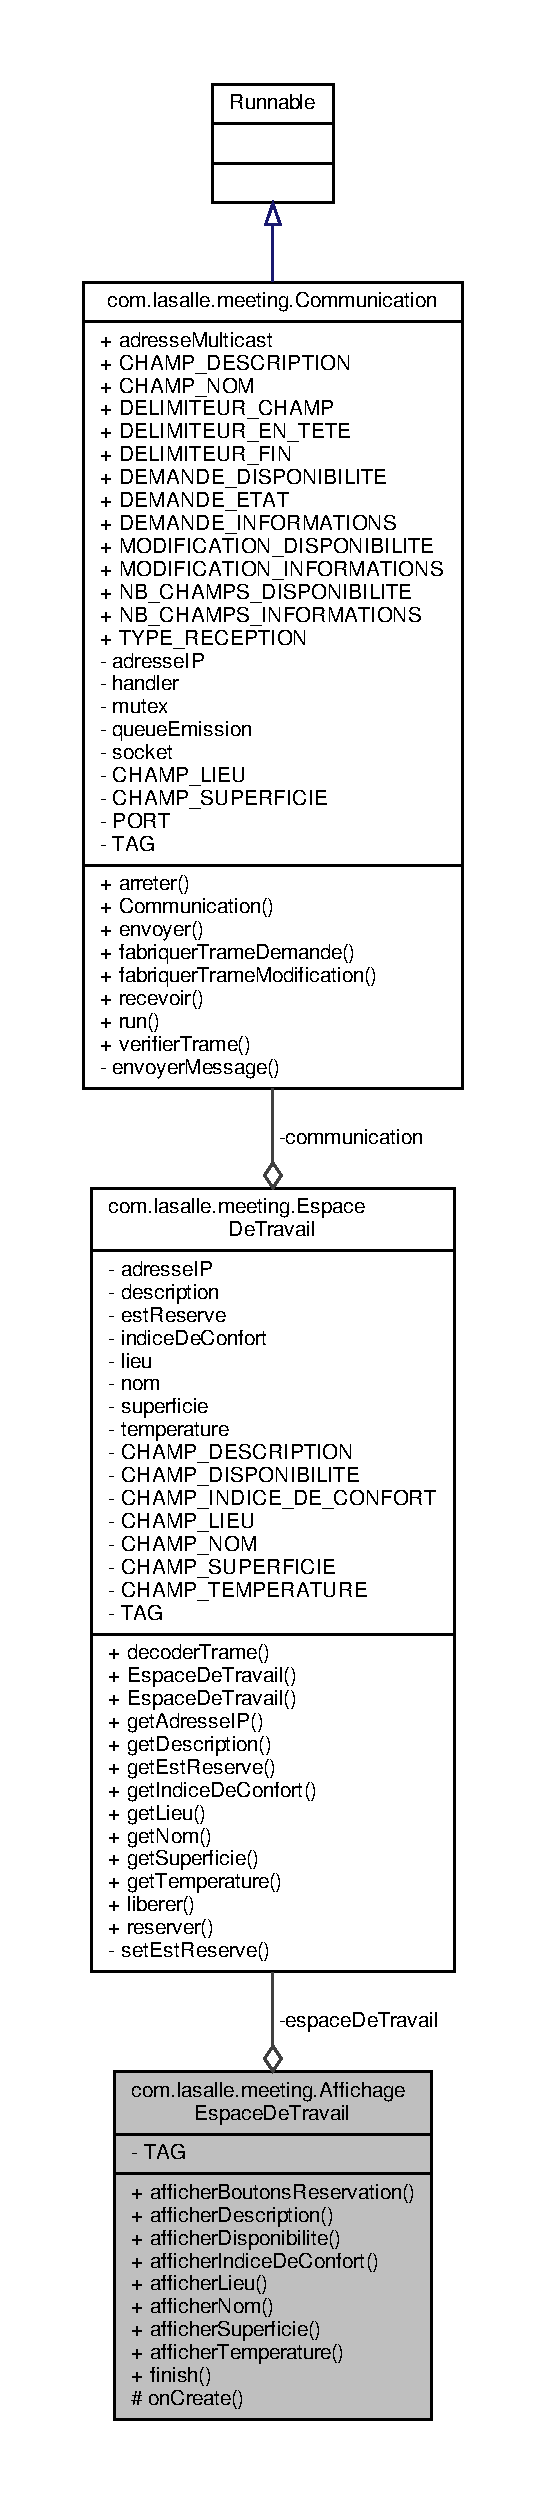
\includegraphics[height=550pt]{classcom_1_1lasalle_1_1meeting_1_1_affichage_espace_de_travail__coll__graph}
\end{center}
\end{figure}
\subsubsection*{Fonctions membres publiques}
\begin{DoxyCompactItemize}
\item 
void \hyperlink{classcom_1_1lasalle_1_1meeting_1_1_affichage_espace_de_travail_a01e3d2585c84043dbe5086a2fc81c371}{afficher\+Boutons\+Reservation} ()
\begin{DoxyCompactList}\small\item\em Affiche les boutons \char`\"{}\+Réserver\char`\"{} et \char`\"{}\+Libérer\char`\"{}. \end{DoxyCompactList}\item 
void \hyperlink{classcom_1_1lasalle_1_1meeting_1_1_affichage_espace_de_travail_a4afb30e3faf37f738f6261fc0696d62b}{afficher\+Description} ()
\begin{DoxyCompactList}\small\item\em Affiche la description de l\textquotesingle{}espace de travail. \end{DoxyCompactList}\item 
void \hyperlink{classcom_1_1lasalle_1_1meeting_1_1_affichage_espace_de_travail_a597703fc6f7e82b79ac7047640fa9323}{afficher\+Disponibilite} ()
\begin{DoxyCompactList}\small\item\em Affiche la disponibilité de l\textquotesingle{}espace de travail. \end{DoxyCompactList}\item 
void \hyperlink{classcom_1_1lasalle_1_1meeting_1_1_affichage_espace_de_travail_acd704eb42f942a10a118d872ffe779a3}{afficher\+Indice\+De\+Confort} ()
\begin{DoxyCompactList}\small\item\em Affiche l\textquotesingle{}indice de confort de l\textquotesingle{}espace de travail. \end{DoxyCompactList}\item 
void \hyperlink{classcom_1_1lasalle_1_1meeting_1_1_affichage_espace_de_travail_a86fc32986ef9ae8f6ef7fca78d91f648}{afficher\+Lieu} ()
\begin{DoxyCompactList}\small\item\em Affiche le lieu de l\textquotesingle{}espace de travail. \end{DoxyCompactList}\item 
void \hyperlink{classcom_1_1lasalle_1_1meeting_1_1_affichage_espace_de_travail_a62159c3fd69a3d4f03306bd3e75c09ce}{afficher\+Nom} ()
\begin{DoxyCompactList}\small\item\em Affiche le nom de l\textquotesingle{}espace de travail. \end{DoxyCompactList}\item 
void \hyperlink{classcom_1_1lasalle_1_1meeting_1_1_affichage_espace_de_travail_ae8f1d5cb6d99aced1996b1b2bbcebe26}{afficher\+Superficie} ()
\begin{DoxyCompactList}\small\item\em Affiche la superficie de l\textquotesingle{}espace de travail. \end{DoxyCompactList}\item 
void \hyperlink{classcom_1_1lasalle_1_1meeting_1_1_affichage_espace_de_travail_a9474bdc380c78e632cc8d384d7393f50}{afficher\+Temperature} ()
\begin{DoxyCompactList}\small\item\em Affiche la température de l\textquotesingle{}espace de travail. \end{DoxyCompactList}\item 
void \hyperlink{classcom_1_1lasalle_1_1meeting_1_1_affichage_espace_de_travail_a2f3649336aff1f2126f817c72faf30c2}{finish} ()
\begin{DoxyCompactList}\small\item\em Termine l\textquotesingle{}activité d\textquotesingle{}affichage d\textquotesingle{}un espace de travail. \end{DoxyCompactList}\end{DoxyCompactItemize}
\subsubsection*{Fonctions membres protégées}
\begin{DoxyCompactItemize}
\item 
void \hyperlink{classcom_1_1lasalle_1_1meeting_1_1_affichage_espace_de_travail_a333ff077dde89888afc62366f6dccf06}{on\+Create} (Bundle saved\+Instance\+State)
\begin{DoxyCompactList}\small\item\em Méthode appelée à la création de l\textquotesingle{}activité \end{DoxyCompactList}\end{DoxyCompactItemize}
\subsubsection*{Attributs privés}
\begin{DoxyCompactItemize}
\item 
\hyperlink{classcom_1_1lasalle_1_1meeting_1_1_espace_de_travail}{Espace\+De\+Travail} \hyperlink{classcom_1_1lasalle_1_1meeting_1_1_affichage_espace_de_travail_a934d41c1c41882b94b65a95cee5aca13}{espace\+De\+Travail}
\end{DoxyCompactItemize}
\subsubsection*{Attributs privés statiques}
\begin{DoxyCompactItemize}
\item 
static final String \hyperlink{classcom_1_1lasalle_1_1meeting_1_1_affichage_espace_de_travail_a8606eb11c7b28f52226544de431d86a4}{T\+AG} = \char`\"{}\+\_\+\+Affichage\+Espace\+Travail\char`\"{}
\end{DoxyCompactItemize}


\subsubsection{Description détaillée}
L\textquotesingle{}activité d\textquotesingle{}affichage d\textquotesingle{}un espace de travail de l\textquotesingle{}application Meeting. 

Définition à la ligne \hyperlink{_affichage_espace_de_travail_8java_source_l00025}{25} du fichier \hyperlink{_affichage_espace_de_travail_8java_source}{Affichage\+Espace\+De\+Travail.\+java}.



\subsubsection{Documentation des fonctions membres}
\mbox{\Hypertarget{classcom_1_1lasalle_1_1meeting_1_1_affichage_espace_de_travail_a01e3d2585c84043dbe5086a2fc81c371}\label{classcom_1_1lasalle_1_1meeting_1_1_affichage_espace_de_travail_a01e3d2585c84043dbe5086a2fc81c371}} 
\index{com\+::lasalle\+::meeting\+::\+Affichage\+Espace\+De\+Travail@{com\+::lasalle\+::meeting\+::\+Affichage\+Espace\+De\+Travail}!afficher\+Boutons\+Reservation@{afficher\+Boutons\+Reservation}}
\index{afficher\+Boutons\+Reservation@{afficher\+Boutons\+Reservation}!com\+::lasalle\+::meeting\+::\+Affichage\+Espace\+De\+Travail@{com\+::lasalle\+::meeting\+::\+Affichage\+Espace\+De\+Travail}}
\paragraph{\texorpdfstring{afficher\+Boutons\+Reservation()}{afficherBoutonsReservation()}}
{\footnotesize\ttfamily void com.\+lasalle.\+meeting.\+Affichage\+Espace\+De\+Travail.\+afficher\+Boutons\+Reservation (\begin{DoxyParamCaption}{ }\end{DoxyParamCaption})}



Affiche les boutons \char`\"{}\+Réserver\char`\"{} et \char`\"{}\+Libérer\char`\"{}. 



Définition à la ligne \hyperlink{_affichage_espace_de_travail_8java_source_l00150}{150} du fichier \hyperlink{_affichage_espace_de_travail_8java_source}{Affichage\+Espace\+De\+Travail.\+java}.



Références \hyperlink{_affichage_espace_de_travail_8java_source_l00127}{com.\+lasalle.\+meeting.\+Affichage\+Espace\+De\+Travail.\+afficher\+Disponibilite()}, \hyperlink{_espace_de_travail_8java_source_l00117}{com.\+lasalle.\+meeting.\+Espace\+De\+Travail.\+get\+Est\+Reserve()}, \hyperlink{_espace_de_travail_8java_source_l00145}{com.\+lasalle.\+meeting.\+Espace\+De\+Travail.\+liberer()}, et \hyperlink{_espace_de_travail_8java_source_l00130}{com.\+lasalle.\+meeting.\+Espace\+De\+Travail.\+reserver()}.



Référencé par \hyperlink{_affichage_espace_de_travail_8java_source_l00041}{com.\+lasalle.\+meeting.\+Affichage\+Espace\+De\+Travail.\+on\+Create()}.


\begin{DoxyCode}
00151     \{
00152         Button boutonReserver = (Button)findViewById(R.id.boutonReserver);
00153         Button boutonLiberer = (Button)findViewById(R.id.boutonLiberer);
00154 
00155         boutonReserver.setOnClickListener(
00156                 \textcolor{keyword}{new} View.OnClickListener()
00157                 \{
00158                     \textcolor{keyword}{public} \textcolor{keywordtype}{void} onClick(View v)
00159                     \{
00160                         \hyperlink{classcom_1_1lasalle_1_1meeting_1_1_affichage_espace_de_travail_a934d41c1c41882b94b65a95cee5aca13}{espaceDeTravail}.\hyperlink{classcom_1_1lasalle_1_1meeting_1_1_espace_de_travail_a42d483a68e6d0d50707dbd3dddd164c2}{reserver}();
00161                         \hyperlink{classcom_1_1lasalle_1_1meeting_1_1_affichage_espace_de_travail_a597703fc6f7e82b79ac7047640fa9323}{afficherDisponibilite}();
00162                         \hyperlink{classcom_1_1lasalle_1_1meeting_1_1_affichage_espace_de_travail_a01e3d2585c84043dbe5086a2fc81c371}{afficherBoutonsReservation}();
00163                     \}
00164                 \}
00165         );
00166 
00167         boutonLiberer.setOnClickListener(
00168                 \textcolor{keyword}{new} View.OnClickListener()
00169                 \{
00170                     \textcolor{keyword}{public} \textcolor{keywordtype}{void} onClick(View v)
00171                     \{
00172                         \hyperlink{classcom_1_1lasalle_1_1meeting_1_1_affichage_espace_de_travail_a934d41c1c41882b94b65a95cee5aca13}{espaceDeTravail}.\hyperlink{classcom_1_1lasalle_1_1meeting_1_1_espace_de_travail_affce017a0a5ba338d7b0b7f6bbce6c68}{liberer}();
00173                         \hyperlink{classcom_1_1lasalle_1_1meeting_1_1_affichage_espace_de_travail_a597703fc6f7e82b79ac7047640fa9323}{afficherDisponibilite}();
00174                         \hyperlink{classcom_1_1lasalle_1_1meeting_1_1_affichage_espace_de_travail_a01e3d2585c84043dbe5086a2fc81c371}{afficherBoutonsReservation}();
00175                     \}
00176                 \}
00177         );
00178 
00179         \textcolor{keywordflow}{if}(!\hyperlink{classcom_1_1lasalle_1_1meeting_1_1_affichage_espace_de_travail_a934d41c1c41882b94b65a95cee5aca13}{espaceDeTravail}.\hyperlink{classcom_1_1lasalle_1_1meeting_1_1_espace_de_travail_a69fe30f8d3aff92986f4c39402e16ab0}{getEstReserve}())
00180         \{
00181             boutonReserver.setVisibility(View.VISIBLE);
00182             boutonLiberer.setVisibility(View.GONE);
00183         \}
00184         \textcolor{keywordflow}{else}
00185         \{
00186             boutonReserver.setVisibility(View.GONE);
00187             boutonLiberer.setVisibility(View.VISIBLE);
00188         \}
00189     \}
\end{DoxyCode}
\mbox{\Hypertarget{classcom_1_1lasalle_1_1meeting_1_1_affichage_espace_de_travail_a4afb30e3faf37f738f6261fc0696d62b}\label{classcom_1_1lasalle_1_1meeting_1_1_affichage_espace_de_travail_a4afb30e3faf37f738f6261fc0696d62b}} 
\index{com\+::lasalle\+::meeting\+::\+Affichage\+Espace\+De\+Travail@{com\+::lasalle\+::meeting\+::\+Affichage\+Espace\+De\+Travail}!afficher\+Description@{afficher\+Description}}
\index{afficher\+Description@{afficher\+Description}!com\+::lasalle\+::meeting\+::\+Affichage\+Espace\+De\+Travail@{com\+::lasalle\+::meeting\+::\+Affichage\+Espace\+De\+Travail}}
\paragraph{\texorpdfstring{afficher\+Description()}{afficherDescription()}}
{\footnotesize\ttfamily void com.\+lasalle.\+meeting.\+Affichage\+Espace\+De\+Travail.\+afficher\+Description (\begin{DoxyParamCaption}{ }\end{DoxyParamCaption})}



Affiche la description de l\textquotesingle{}espace de travail. 



Définition à la ligne \hyperlink{_affichage_espace_de_travail_8java_source_l00083}{83} du fichier \hyperlink{_affichage_espace_de_travail_8java_source}{Affichage\+Espace\+De\+Travail.\+java}.



Références \hyperlink{_espace_de_travail_8java_source_l00097}{com.\+lasalle.\+meeting.\+Espace\+De\+Travail.\+get\+Description()}.



Référencé par \hyperlink{_affichage_espace_de_travail_8java_source_l00041}{com.\+lasalle.\+meeting.\+Affichage\+Espace\+De\+Travail.\+on\+Create()}.


\begin{DoxyCode}
00084     \{
00085         TextView affichageDescription = (TextView)findViewById(R.id.affichageDescription);
00086         affichageDescription.setText(\hyperlink{classcom_1_1lasalle_1_1meeting_1_1_affichage_espace_de_travail_a934d41c1c41882b94b65a95cee5aca13}{espaceDeTravail}.
      \hyperlink{classcom_1_1lasalle_1_1meeting_1_1_espace_de_travail_a815ecee3f01117f2d9b1d9441b214907}{getDescription}());
00087 
00088         Log.d(\hyperlink{classcom_1_1lasalle_1_1meeting_1_1_affichage_espace_de_travail_a8606eb11c7b28f52226544de431d86a4}{TAG}, \textcolor{stringliteral}{"afficherDescription() "} + \hyperlink{classcom_1_1lasalle_1_1meeting_1_1_affichage_espace_de_travail_a934d41c1c41882b94b65a95cee5aca13}{espaceDeTravail}.
      \hyperlink{classcom_1_1lasalle_1_1meeting_1_1_espace_de_travail_a815ecee3f01117f2d9b1d9441b214907}{getDescription}());
00089     \}
\end{DoxyCode}
\mbox{\Hypertarget{classcom_1_1lasalle_1_1meeting_1_1_affichage_espace_de_travail_a597703fc6f7e82b79ac7047640fa9323}\label{classcom_1_1lasalle_1_1meeting_1_1_affichage_espace_de_travail_a597703fc6f7e82b79ac7047640fa9323}} 
\index{com\+::lasalle\+::meeting\+::\+Affichage\+Espace\+De\+Travail@{com\+::lasalle\+::meeting\+::\+Affichage\+Espace\+De\+Travail}!afficher\+Disponibilite@{afficher\+Disponibilite}}
\index{afficher\+Disponibilite@{afficher\+Disponibilite}!com\+::lasalle\+::meeting\+::\+Affichage\+Espace\+De\+Travail@{com\+::lasalle\+::meeting\+::\+Affichage\+Espace\+De\+Travail}}
\paragraph{\texorpdfstring{afficher\+Disponibilite()}{afficherDisponibilite()}}
{\footnotesize\ttfamily void com.\+lasalle.\+meeting.\+Affichage\+Espace\+De\+Travail.\+afficher\+Disponibilite (\begin{DoxyParamCaption}{ }\end{DoxyParamCaption})}



Affiche la disponibilité de l\textquotesingle{}espace de travail. 



Définition à la ligne \hyperlink{_affichage_espace_de_travail_8java_source_l00127}{127} du fichier \hyperlink{_affichage_espace_de_travail_8java_source}{Affichage\+Espace\+De\+Travail.\+java}.



Références \hyperlink{_espace_de_travail_8java_source_l00117}{com.\+lasalle.\+meeting.\+Espace\+De\+Travail.\+get\+Est\+Reserve()}.



Référencé par \hyperlink{_affichage_espace_de_travail_8java_source_l00150}{com.\+lasalle.\+meeting.\+Affichage\+Espace\+De\+Travail.\+afficher\+Boutons\+Reservation()}, et \hyperlink{_affichage_espace_de_travail_8java_source_l00041}{com.\+lasalle.\+meeting.\+Affichage\+Espace\+De\+Travail.\+on\+Create()}.


\begin{DoxyCode}
00128     \{
00129         TextView affichageDisponibilite = (TextView)findViewById(R.id.affichageDisponibilite);
00130 
00131         \textcolor{keywordflow}{if}(!\hyperlink{classcom_1_1lasalle_1_1meeting_1_1_affichage_espace_de_travail_a934d41c1c41882b94b65a95cee5aca13}{espaceDeTravail}.\hyperlink{classcom_1_1lasalle_1_1meeting_1_1_espace_de_travail_a69fe30f8d3aff92986f4c39402e16ab0}{getEstReserve}())
00132         \{
00133             Log.d(\hyperlink{classcom_1_1lasalle_1_1meeting_1_1_affichage_espace_de_travail_a8606eb11c7b28f52226544de431d86a4}{TAG}, \textcolor{stringliteral}{"Libre"});
00134             affichageDisponibilite.setText(\textcolor{stringliteral}{"Libre"});
00135             affichageDisponibilite.setTextColor(Color.parseColor(\textcolor{stringliteral}{"#00FF00"})); \textcolor{comment}{// Color.rgb(0,255,0)}
00136         \}
00137         \textcolor{keywordflow}{else}
00138         \{
00139             Log.d(\hyperlink{classcom_1_1lasalle_1_1meeting_1_1_affichage_espace_de_travail_a8606eb11c7b28f52226544de431d86a4}{TAG}, \textcolor{stringliteral}{"Occupé"});
00140             affichageDisponibilite.setText(\textcolor{stringliteral}{"Occupé"});
00141             affichageDisponibilite.setTextColor(Color.rgb(255,0,0));
00142         \}
00143 
00144         Log.d(\hyperlink{classcom_1_1lasalle_1_1meeting_1_1_affichage_espace_de_travail_a8606eb11c7b28f52226544de431d86a4}{TAG}, \textcolor{stringliteral}{"afficherDisponibilite() "} + \hyperlink{classcom_1_1lasalle_1_1meeting_1_1_affichage_espace_de_travail_a934d41c1c41882b94b65a95cee5aca13}{espaceDeTravail}.
      \hyperlink{classcom_1_1lasalle_1_1meeting_1_1_espace_de_travail_a69fe30f8d3aff92986f4c39402e16ab0}{getEstReserve}());
00145     \}
\end{DoxyCode}
\mbox{\Hypertarget{classcom_1_1lasalle_1_1meeting_1_1_affichage_espace_de_travail_acd704eb42f942a10a118d872ffe779a3}\label{classcom_1_1lasalle_1_1meeting_1_1_affichage_espace_de_travail_acd704eb42f942a10a118d872ffe779a3}} 
\index{com\+::lasalle\+::meeting\+::\+Affichage\+Espace\+De\+Travail@{com\+::lasalle\+::meeting\+::\+Affichage\+Espace\+De\+Travail}!afficher\+Indice\+De\+Confort@{afficher\+Indice\+De\+Confort}}
\index{afficher\+Indice\+De\+Confort@{afficher\+Indice\+De\+Confort}!com\+::lasalle\+::meeting\+::\+Affichage\+Espace\+De\+Travail@{com\+::lasalle\+::meeting\+::\+Affichage\+Espace\+De\+Travail}}
\paragraph{\texorpdfstring{afficher\+Indice\+De\+Confort()}{afficherIndiceDeConfort()}}
{\footnotesize\ttfamily void com.\+lasalle.\+meeting.\+Affichage\+Espace\+De\+Travail.\+afficher\+Indice\+De\+Confort (\begin{DoxyParamCaption}{ }\end{DoxyParamCaption})}



Affiche l\textquotesingle{}indice de confort de l\textquotesingle{}espace de travail. 



Définition à la ligne \hyperlink{_affichage_espace_de_travail_8java_source_l00116}{116} du fichier \hyperlink{_affichage_espace_de_travail_8java_source}{Affichage\+Espace\+De\+Travail.\+java}.



Références \hyperlink{_espace_de_travail_8java_source_l00112}{com.\+lasalle.\+meeting.\+Espace\+De\+Travail.\+get\+Indice\+De\+Confort()}.



Référencé par \hyperlink{_affichage_espace_de_travail_8java_source_l00041}{com.\+lasalle.\+meeting.\+Affichage\+Espace\+De\+Travail.\+on\+Create()}.


\begin{DoxyCode}
00117     \{
00118         TextView affichageIndiceDeConfort = (TextView)findViewById(R.id.affichageIndiceDeConfort);
00119         affichageIndiceDeConfort.setText(String.valueOf(\hyperlink{classcom_1_1lasalle_1_1meeting_1_1_affichage_espace_de_travail_a934d41c1c41882b94b65a95cee5aca13}{espaceDeTravail}.
      \hyperlink{classcom_1_1lasalle_1_1meeting_1_1_espace_de_travail_a9d7b3bd8aa78a10c70851b477d0f522d}{getIndiceDeConfort}()));
00120 
00121         Log.d(\hyperlink{classcom_1_1lasalle_1_1meeting_1_1_affichage_espace_de_travail_a8606eb11c7b28f52226544de431d86a4}{TAG}, \textcolor{stringliteral}{"afficherIndiceDeConfort() "} + \hyperlink{classcom_1_1lasalle_1_1meeting_1_1_affichage_espace_de_travail_a934d41c1c41882b94b65a95cee5aca13}{espaceDeTravail}.
      \hyperlink{classcom_1_1lasalle_1_1meeting_1_1_espace_de_travail_a9d7b3bd8aa78a10c70851b477d0f522d}{getIndiceDeConfort}());
00122     \}
\end{DoxyCode}
\mbox{\Hypertarget{classcom_1_1lasalle_1_1meeting_1_1_affichage_espace_de_travail_a86fc32986ef9ae8f6ef7fca78d91f648}\label{classcom_1_1lasalle_1_1meeting_1_1_affichage_espace_de_travail_a86fc32986ef9ae8f6ef7fca78d91f648}} 
\index{com\+::lasalle\+::meeting\+::\+Affichage\+Espace\+De\+Travail@{com\+::lasalle\+::meeting\+::\+Affichage\+Espace\+De\+Travail}!afficher\+Lieu@{afficher\+Lieu}}
\index{afficher\+Lieu@{afficher\+Lieu}!com\+::lasalle\+::meeting\+::\+Affichage\+Espace\+De\+Travail@{com\+::lasalle\+::meeting\+::\+Affichage\+Espace\+De\+Travail}}
\paragraph{\texorpdfstring{afficher\+Lieu()}{afficherLieu()}}
{\footnotesize\ttfamily void com.\+lasalle.\+meeting.\+Affichage\+Espace\+De\+Travail.\+afficher\+Lieu (\begin{DoxyParamCaption}{ }\end{DoxyParamCaption})}



Affiche le lieu de l\textquotesingle{}espace de travail. 



Définition à la ligne \hyperlink{_affichage_espace_de_travail_8java_source_l00072}{72} du fichier \hyperlink{_affichage_espace_de_travail_8java_source}{Affichage\+Espace\+De\+Travail.\+java}.



Références \hyperlink{_espace_de_travail_8java_source_l00092}{com.\+lasalle.\+meeting.\+Espace\+De\+Travail.\+get\+Lieu()}.



Référencé par \hyperlink{_affichage_espace_de_travail_8java_source_l00041}{com.\+lasalle.\+meeting.\+Affichage\+Espace\+De\+Travail.\+on\+Create()}.


\begin{DoxyCode}
00073     \{
00074         TextView affichageLieu = (TextView)findViewById(R.id.affichageLieu);
00075         affichageLieu.setText(\hyperlink{classcom_1_1lasalle_1_1meeting_1_1_affichage_espace_de_travail_a934d41c1c41882b94b65a95cee5aca13}{espaceDeTravail}.\hyperlink{classcom_1_1lasalle_1_1meeting_1_1_espace_de_travail_af320aa4ad7711ed52b3b5aef1bd52dd1}{getLieu}());
00076 
00077         Log.d(\hyperlink{classcom_1_1lasalle_1_1meeting_1_1_affichage_espace_de_travail_a8606eb11c7b28f52226544de431d86a4}{TAG}, \textcolor{stringliteral}{"afficherLieu() "} + \hyperlink{classcom_1_1lasalle_1_1meeting_1_1_affichage_espace_de_travail_a934d41c1c41882b94b65a95cee5aca13}{espaceDeTravail}.\hyperlink{classcom_1_1lasalle_1_1meeting_1_1_espace_de_travail_af320aa4ad7711ed52b3b5aef1bd52dd1}{getLieu}());
00078     \}
\end{DoxyCode}
\mbox{\Hypertarget{classcom_1_1lasalle_1_1meeting_1_1_affichage_espace_de_travail_a62159c3fd69a3d4f03306bd3e75c09ce}\label{classcom_1_1lasalle_1_1meeting_1_1_affichage_espace_de_travail_a62159c3fd69a3d4f03306bd3e75c09ce}} 
\index{com\+::lasalle\+::meeting\+::\+Affichage\+Espace\+De\+Travail@{com\+::lasalle\+::meeting\+::\+Affichage\+Espace\+De\+Travail}!afficher\+Nom@{afficher\+Nom}}
\index{afficher\+Nom@{afficher\+Nom}!com\+::lasalle\+::meeting\+::\+Affichage\+Espace\+De\+Travail@{com\+::lasalle\+::meeting\+::\+Affichage\+Espace\+De\+Travail}}
\paragraph{\texorpdfstring{afficher\+Nom()}{afficherNom()}}
{\footnotesize\ttfamily void com.\+lasalle.\+meeting.\+Affichage\+Espace\+De\+Travail.\+afficher\+Nom (\begin{DoxyParamCaption}{ }\end{DoxyParamCaption})}



Affiche le nom de l\textquotesingle{}espace de travail. 



Définition à la ligne \hyperlink{_affichage_espace_de_travail_8java_source_l00061}{61} du fichier \hyperlink{_affichage_espace_de_travail_8java_source}{Affichage\+Espace\+De\+Travail.\+java}.



Références \hyperlink{_espace_de_travail_8java_source_l00087}{com.\+lasalle.\+meeting.\+Espace\+De\+Travail.\+get\+Nom()}.



Référencé par \hyperlink{_affichage_espace_de_travail_8java_source_l00041}{com.\+lasalle.\+meeting.\+Affichage\+Espace\+De\+Travail.\+on\+Create()}.


\begin{DoxyCode}
00062     \{
00063         TextView affichageNom = (TextView)findViewById(R.id.affichageNom);
00064         affichageNom.setText(\hyperlink{classcom_1_1lasalle_1_1meeting_1_1_affichage_espace_de_travail_a934d41c1c41882b94b65a95cee5aca13}{espaceDeTravail}.\hyperlink{classcom_1_1lasalle_1_1meeting_1_1_espace_de_travail_ae662e2674616a8548755cb64a38e0432}{getNom}());
00065 
00066         Log.d(\hyperlink{classcom_1_1lasalle_1_1meeting_1_1_affichage_espace_de_travail_a8606eb11c7b28f52226544de431d86a4}{TAG}, \textcolor{stringliteral}{"afficherNom() "} + \hyperlink{classcom_1_1lasalle_1_1meeting_1_1_affichage_espace_de_travail_a934d41c1c41882b94b65a95cee5aca13}{espaceDeTravail}.\hyperlink{classcom_1_1lasalle_1_1meeting_1_1_espace_de_travail_ae662e2674616a8548755cb64a38e0432}{getNom}());
00067     \}
\end{DoxyCode}
\mbox{\Hypertarget{classcom_1_1lasalle_1_1meeting_1_1_affichage_espace_de_travail_ae8f1d5cb6d99aced1996b1b2bbcebe26}\label{classcom_1_1lasalle_1_1meeting_1_1_affichage_espace_de_travail_ae8f1d5cb6d99aced1996b1b2bbcebe26}} 
\index{com\+::lasalle\+::meeting\+::\+Affichage\+Espace\+De\+Travail@{com\+::lasalle\+::meeting\+::\+Affichage\+Espace\+De\+Travail}!afficher\+Superficie@{afficher\+Superficie}}
\index{afficher\+Superficie@{afficher\+Superficie}!com\+::lasalle\+::meeting\+::\+Affichage\+Espace\+De\+Travail@{com\+::lasalle\+::meeting\+::\+Affichage\+Espace\+De\+Travail}}
\paragraph{\texorpdfstring{afficher\+Superficie()}{afficherSuperficie()}}
{\footnotesize\ttfamily void com.\+lasalle.\+meeting.\+Affichage\+Espace\+De\+Travail.\+afficher\+Superficie (\begin{DoxyParamCaption}{ }\end{DoxyParamCaption})}



Affiche la superficie de l\textquotesingle{}espace de travail. 



Définition à la ligne \hyperlink{_affichage_espace_de_travail_8java_source_l00094}{94} du fichier \hyperlink{_affichage_espace_de_travail_8java_source}{Affichage\+Espace\+De\+Travail.\+java}.



Références \hyperlink{_espace_de_travail_8java_source_l00102}{com.\+lasalle.\+meeting.\+Espace\+De\+Travail.\+get\+Superficie()}.



Référencé par \hyperlink{_affichage_espace_de_travail_8java_source_l00041}{com.\+lasalle.\+meeting.\+Affichage\+Espace\+De\+Travail.\+on\+Create()}.


\begin{DoxyCode}
00095     \{
00096         TextView affichageSuperficie = (TextView)findViewById(R.id.affichageSuperficie);
00097         affichageSuperficie.setText(String.valueOf(\hyperlink{classcom_1_1lasalle_1_1meeting_1_1_affichage_espace_de_travail_a934d41c1c41882b94b65a95cee5aca13}{espaceDeTravail}.
      \hyperlink{classcom_1_1lasalle_1_1meeting_1_1_espace_de_travail_ae2c734da9d454b368ddb056b1cdae499}{getSuperficie}()));
00098 
00099         Log.d(\hyperlink{classcom_1_1lasalle_1_1meeting_1_1_affichage_espace_de_travail_a8606eb11c7b28f52226544de431d86a4}{TAG}, \textcolor{stringliteral}{"afficherSuperficie() "} + \hyperlink{classcom_1_1lasalle_1_1meeting_1_1_affichage_espace_de_travail_a934d41c1c41882b94b65a95cee5aca13}{espaceDeTravail}.
      \hyperlink{classcom_1_1lasalle_1_1meeting_1_1_espace_de_travail_ae2c734da9d454b368ddb056b1cdae499}{getSuperficie}());
00100     \}
\end{DoxyCode}
\mbox{\Hypertarget{classcom_1_1lasalle_1_1meeting_1_1_affichage_espace_de_travail_a9474bdc380c78e632cc8d384d7393f50}\label{classcom_1_1lasalle_1_1meeting_1_1_affichage_espace_de_travail_a9474bdc380c78e632cc8d384d7393f50}} 
\index{com\+::lasalle\+::meeting\+::\+Affichage\+Espace\+De\+Travail@{com\+::lasalle\+::meeting\+::\+Affichage\+Espace\+De\+Travail}!afficher\+Temperature@{afficher\+Temperature}}
\index{afficher\+Temperature@{afficher\+Temperature}!com\+::lasalle\+::meeting\+::\+Affichage\+Espace\+De\+Travail@{com\+::lasalle\+::meeting\+::\+Affichage\+Espace\+De\+Travail}}
\paragraph{\texorpdfstring{afficher\+Temperature()}{afficherTemperature()}}
{\footnotesize\ttfamily void com.\+lasalle.\+meeting.\+Affichage\+Espace\+De\+Travail.\+afficher\+Temperature (\begin{DoxyParamCaption}{ }\end{DoxyParamCaption})}



Affiche la température de l\textquotesingle{}espace de travail. 



Définition à la ligne \hyperlink{_affichage_espace_de_travail_8java_source_l00105}{105} du fichier \hyperlink{_affichage_espace_de_travail_8java_source}{Affichage\+Espace\+De\+Travail.\+java}.



Références \hyperlink{_espace_de_travail_8java_source_l00107}{com.\+lasalle.\+meeting.\+Espace\+De\+Travail.\+get\+Temperature()}.



Référencé par \hyperlink{_affichage_espace_de_travail_8java_source_l00041}{com.\+lasalle.\+meeting.\+Affichage\+Espace\+De\+Travail.\+on\+Create()}.


\begin{DoxyCode}
00106     \{
00107         TextView affichageTemperature = (TextView)findViewById(R.id.affichageTemperature);
00108         affichageTemperature.setText(String.valueOf(\hyperlink{classcom_1_1lasalle_1_1meeting_1_1_affichage_espace_de_travail_a934d41c1c41882b94b65a95cee5aca13}{espaceDeTravail}.
      \hyperlink{classcom_1_1lasalle_1_1meeting_1_1_espace_de_travail_a4c01c37fa6431d48c59274aaa00fdbe3}{getTemperature}()));
00109 
00110         Log.d(\hyperlink{classcom_1_1lasalle_1_1meeting_1_1_affichage_espace_de_travail_a8606eb11c7b28f52226544de431d86a4}{TAG}, \textcolor{stringliteral}{"afficherTemperature() "} + \hyperlink{classcom_1_1lasalle_1_1meeting_1_1_affichage_espace_de_travail_a934d41c1c41882b94b65a95cee5aca13}{espaceDeTravail}.
      \hyperlink{classcom_1_1lasalle_1_1meeting_1_1_espace_de_travail_a4c01c37fa6431d48c59274aaa00fdbe3}{getTemperature}());
00111     \}
\end{DoxyCode}
\mbox{\Hypertarget{classcom_1_1lasalle_1_1meeting_1_1_affichage_espace_de_travail_a2f3649336aff1f2126f817c72faf30c2}\label{classcom_1_1lasalle_1_1meeting_1_1_affichage_espace_de_travail_a2f3649336aff1f2126f817c72faf30c2}} 
\index{com\+::lasalle\+::meeting\+::\+Affichage\+Espace\+De\+Travail@{com\+::lasalle\+::meeting\+::\+Affichage\+Espace\+De\+Travail}!finish@{finish}}
\index{finish@{finish}!com\+::lasalle\+::meeting\+::\+Affichage\+Espace\+De\+Travail@{com\+::lasalle\+::meeting\+::\+Affichage\+Espace\+De\+Travail}}
\paragraph{\texorpdfstring{finish()}{finish()}}
{\footnotesize\ttfamily void com.\+lasalle.\+meeting.\+Affichage\+Espace\+De\+Travail.\+finish (\begin{DoxyParamCaption}{ }\end{DoxyParamCaption})}



Termine l\textquotesingle{}activité d\textquotesingle{}affichage d\textquotesingle{}un espace de travail. 



Définition à la ligne \hyperlink{_affichage_espace_de_travail_8java_source_l00195}{195} du fichier \hyperlink{_affichage_espace_de_travail_8java_source}{Affichage\+Espace\+De\+Travail.\+java}.


\begin{DoxyCode}
00196     \{
00197         Log.d(\hyperlink{classcom_1_1lasalle_1_1meeting_1_1_affichage_espace_de_travail_a8606eb11c7b28f52226544de431d86a4}{TAG}, \textcolor{stringliteral}{"finish()"});
00198 
00199         Intent intent = \textcolor{keyword}{new} Intent();
00200         intent.putExtra(\textcolor{stringliteral}{"unEspaceDeTravail"}, \hyperlink{classcom_1_1lasalle_1_1meeting_1_1_affichage_espace_de_travail_a934d41c1c41882b94b65a95cee5aca13}{espaceDeTravail});
00201 
00202         setResult(RESULT\_OK, intent);
00203         super.finish();
00204     \}
\end{DoxyCode}
\mbox{\Hypertarget{classcom_1_1lasalle_1_1meeting_1_1_affichage_espace_de_travail_a333ff077dde89888afc62366f6dccf06}\label{classcom_1_1lasalle_1_1meeting_1_1_affichage_espace_de_travail_a333ff077dde89888afc62366f6dccf06}} 
\index{com\+::lasalle\+::meeting\+::\+Affichage\+Espace\+De\+Travail@{com\+::lasalle\+::meeting\+::\+Affichage\+Espace\+De\+Travail}!on\+Create@{on\+Create}}
\index{on\+Create@{on\+Create}!com\+::lasalle\+::meeting\+::\+Affichage\+Espace\+De\+Travail@{com\+::lasalle\+::meeting\+::\+Affichage\+Espace\+De\+Travail}}
\paragraph{\texorpdfstring{on\+Create()}{onCreate()}}
{\footnotesize\ttfamily void com.\+lasalle.\+meeting.\+Affichage\+Espace\+De\+Travail.\+on\+Create (\begin{DoxyParamCaption}\item[{Bundle}]{saved\+Instance\+State }\end{DoxyParamCaption})\hspace{0.3cm}{\ttfamily [protected]}}



Méthode appelée à la création de l\textquotesingle{}activité 



Définition à la ligne \hyperlink{_affichage_espace_de_travail_8java_source_l00041}{41} du fichier \hyperlink{_affichage_espace_de_travail_8java_source}{Affichage\+Espace\+De\+Travail.\+java}.



Références \hyperlink{_affichage_espace_de_travail_8java_source_l00150}{com.\+lasalle.\+meeting.\+Affichage\+Espace\+De\+Travail.\+afficher\+Boutons\+Reservation()}, \hyperlink{_affichage_espace_de_travail_8java_source_l00083}{com.\+lasalle.\+meeting.\+Affichage\+Espace\+De\+Travail.\+afficher\+Description()}, \hyperlink{_affichage_espace_de_travail_8java_source_l00127}{com.\+lasalle.\+meeting.\+Affichage\+Espace\+De\+Travail.\+afficher\+Disponibilite()}, \hyperlink{_affichage_espace_de_travail_8java_source_l00116}{com.\+lasalle.\+meeting.\+Affichage\+Espace\+De\+Travail.\+afficher\+Indice\+De\+Confort()}, \hyperlink{_affichage_espace_de_travail_8java_source_l00072}{com.\+lasalle.\+meeting.\+Affichage\+Espace\+De\+Travail.\+afficher\+Lieu()}, \hyperlink{_affichage_espace_de_travail_8java_source_l00061}{com.\+lasalle.\+meeting.\+Affichage\+Espace\+De\+Travail.\+afficher\+Nom()}, \hyperlink{_affichage_espace_de_travail_8java_source_l00094}{com.\+lasalle.\+meeting.\+Affichage\+Espace\+De\+Travail.\+afficher\+Superficie()}, et \hyperlink{_affichage_espace_de_travail_8java_source_l00105}{com.\+lasalle.\+meeting.\+Affichage\+Espace\+De\+Travail.\+afficher\+Temperature()}.


\begin{DoxyCode}
00042     \{
00043         super.onCreate(savedInstanceState);
00044         setContentView(R.layout.activity\_affichage\_espace\_de\_travail);
00045         Intent intent = getIntent();
00046         \hyperlink{classcom_1_1lasalle_1_1meeting_1_1_affichage_espace_de_travail_a934d41c1c41882b94b65a95cee5aca13}{espaceDeTravail} = (EspaceDeTravail)intent.getSerializableExtra(\textcolor{stringliteral}{"unEspaceDeTravail"});
00047 
00048         \hyperlink{classcom_1_1lasalle_1_1meeting_1_1_affichage_espace_de_travail_a62159c3fd69a3d4f03306bd3e75c09ce}{afficherNom}();
00049         \hyperlink{classcom_1_1lasalle_1_1meeting_1_1_affichage_espace_de_travail_a86fc32986ef9ae8f6ef7fca78d91f648}{afficherLieu}();
00050         \hyperlink{classcom_1_1lasalle_1_1meeting_1_1_affichage_espace_de_travail_a4afb30e3faf37f738f6261fc0696d62b}{afficherDescription}();
00051         \hyperlink{classcom_1_1lasalle_1_1meeting_1_1_affichage_espace_de_travail_ae8f1d5cb6d99aced1996b1b2bbcebe26}{afficherSuperficie}();
00052         \hyperlink{classcom_1_1lasalle_1_1meeting_1_1_affichage_espace_de_travail_a9474bdc380c78e632cc8d384d7393f50}{afficherTemperature}();
00053         \hyperlink{classcom_1_1lasalle_1_1meeting_1_1_affichage_espace_de_travail_acd704eb42f942a10a118d872ffe779a3}{afficherIndiceDeConfort}();
00054         \hyperlink{classcom_1_1lasalle_1_1meeting_1_1_affichage_espace_de_travail_a597703fc6f7e82b79ac7047640fa9323}{afficherDisponibilite}();
00055         \hyperlink{classcom_1_1lasalle_1_1meeting_1_1_affichage_espace_de_travail_a01e3d2585c84043dbe5086a2fc81c371}{afficherBoutonsReservation}();
00056     \}
\end{DoxyCode}


\subsubsection{Documentation des données membres}
\mbox{\Hypertarget{classcom_1_1lasalle_1_1meeting_1_1_affichage_espace_de_travail_a934d41c1c41882b94b65a95cee5aca13}\label{classcom_1_1lasalle_1_1meeting_1_1_affichage_espace_de_travail_a934d41c1c41882b94b65a95cee5aca13}} 
\index{com\+::lasalle\+::meeting\+::\+Affichage\+Espace\+De\+Travail@{com\+::lasalle\+::meeting\+::\+Affichage\+Espace\+De\+Travail}!espace\+De\+Travail@{espace\+De\+Travail}}
\index{espace\+De\+Travail@{espace\+De\+Travail}!com\+::lasalle\+::meeting\+::\+Affichage\+Espace\+De\+Travail@{com\+::lasalle\+::meeting\+::\+Affichage\+Espace\+De\+Travail}}
\paragraph{\texorpdfstring{espace\+De\+Travail}{espaceDeTravail}}
{\footnotesize\ttfamily \hyperlink{classcom_1_1lasalle_1_1meeting_1_1_espace_de_travail}{Espace\+De\+Travail} com.\+lasalle.\+meeting.\+Affichage\+Espace\+De\+Travail.\+espace\+De\+Travail\hspace{0.3cm}{\ttfamily [private]}}

Les attributs 

Définition à la ligne \hyperlink{_affichage_espace_de_travail_8java_source_l00035}{35} du fichier \hyperlink{_affichage_espace_de_travail_8java_source}{Affichage\+Espace\+De\+Travail.\+java}.

\mbox{\Hypertarget{classcom_1_1lasalle_1_1meeting_1_1_affichage_espace_de_travail_a8606eb11c7b28f52226544de431d86a4}\label{classcom_1_1lasalle_1_1meeting_1_1_affichage_espace_de_travail_a8606eb11c7b28f52226544de431d86a4}} 
\index{com\+::lasalle\+::meeting\+::\+Affichage\+Espace\+De\+Travail@{com\+::lasalle\+::meeting\+::\+Affichage\+Espace\+De\+Travail}!T\+AG@{T\+AG}}
\index{T\+AG@{T\+AG}!com\+::lasalle\+::meeting\+::\+Affichage\+Espace\+De\+Travail@{com\+::lasalle\+::meeting\+::\+Affichage\+Espace\+De\+Travail}}
\paragraph{\texorpdfstring{T\+AG}{TAG}}
{\footnotesize\ttfamily final String com.\+lasalle.\+meeting.\+Affichage\+Espace\+De\+Travail.\+T\+AG = \char`\"{}\+\_\+\+Affichage\+Espace\+Travail\char`\"{}\hspace{0.3cm}{\ttfamily [static]}, {\ttfamily [private]}}

Les constantes 

Définition à la ligne \hyperlink{_affichage_espace_de_travail_8java_source_l00030}{30} du fichier \hyperlink{_affichage_espace_de_travail_8java_source}{Affichage\+Espace\+De\+Travail.\+java}.



La documentation de cette classe a été générée à partir du fichier suivant \+:\begin{DoxyCompactItemize}
\item 
\hyperlink{_affichage_espace_de_travail_8java}{Affichage\+Espace\+De\+Travail.\+java}\end{DoxyCompactItemize}

\hypertarget{classcom_1_1lasalle_1_1meeting_1_1_communication}{}\subsection{Référence de la classe com.\+lasalle.\+meeting.\+Communication}
\label{classcom_1_1lasalle_1_1meeting_1_1_communication}\index{com.\+lasalle.\+meeting.\+Communication@{com.\+lasalle.\+meeting.\+Communication}}


\hyperlink{classcom_1_1lasalle_1_1meeting_1_1_communication}{Communication} entre l\textquotesingle{}application et le portier.  




Graphe de collaboration de com.\+lasalle.\+meeting.\+Communication\+:\nopagebreak
\begin{figure}[H]
\begin{center}
\leavevmode
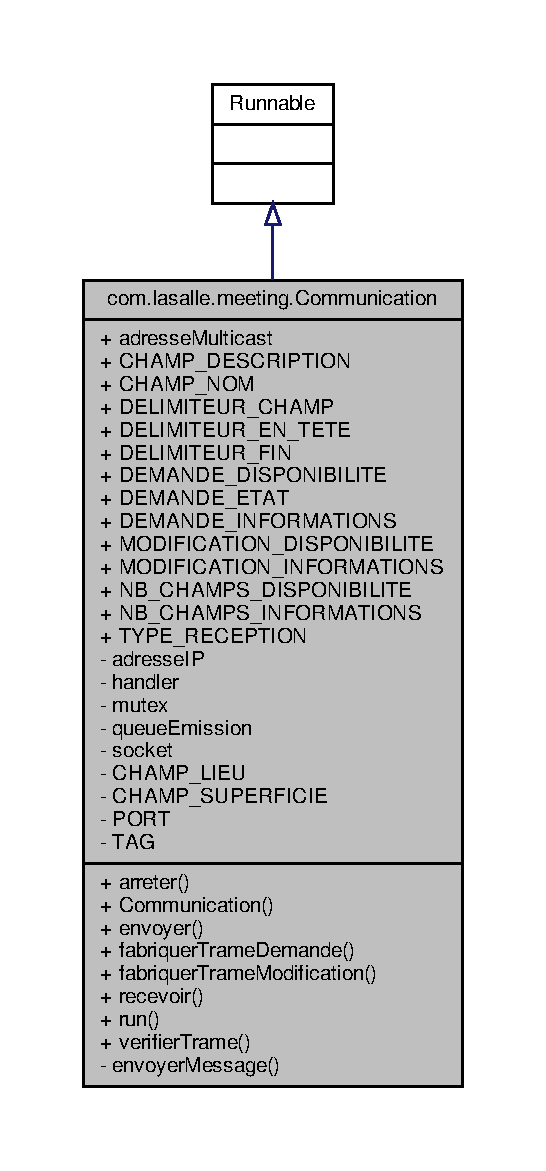
\includegraphics[height=550pt]{classcom_1_1lasalle_1_1meeting_1_1_communication__coll__graph}
\end{center}
\end{figure}
\subsubsection*{Fonctions membres publiques}
\begin{DoxyCompactItemize}
\item 
void \hyperlink{classcom_1_1lasalle_1_1meeting_1_1_communication_abf23e6b879122267b3fe10233b4010a8}{arreter} ()
\begin{DoxyCompactList}\small\item\em méthode arrétant la socket, donc la communication avec les portiers \end{DoxyCompactList}\item 
\hyperlink{classcom_1_1lasalle_1_1meeting_1_1_communication_a3d73554b2774d3274ad385b0faa27d14}{Communication} (Handler \hyperlink{classcom_1_1lasalle_1_1meeting_1_1_communication_a05fa5f360f28819a9e106e0265a74643}{handler})
\begin{DoxyCompactList}\small\item\em Constructeur par défaut de la classe \hyperlink{classcom_1_1lasalle_1_1meeting_1_1_communication}{Communication}. \end{DoxyCompactList}\item 
void \hyperlink{classcom_1_1lasalle_1_1meeting_1_1_communication_a03f0e419513d7f33900dde412e2a4471}{envoyer} (String trame, String adresse\+Portier)
\begin{DoxyCompactList}\small\item\em Envoie la trame. \end{DoxyCompactList}\item 
String \hyperlink{classcom_1_1lasalle_1_1meeting_1_1_communication_a3b07023cb3f3a1549da711b5c6ba6af1}{fabriquer\+Trame\+Demande} (int type\+Trame)
\begin{DoxyCompactList}\small\item\em Fabrique la trame de demande. \end{DoxyCompactList}\item 
String \hyperlink{classcom_1_1lasalle_1_1meeting_1_1_communication_a82b49090e24d8296bfd26a14e0951ade}{fabriquer\+Trame\+Modification} (int type\+Trame, List$<$ String $>$ parametres)
\begin{DoxyCompactList}\small\item\em Fabrique la trame de modification. \end{DoxyCompactList}\item 
void \hyperlink{classcom_1_1lasalle_1_1meeting_1_1_communication_a0344b79faa04dded3468fb8dda6baa81}{recevoir} ()
\begin{DoxyCompactList}\small\item\em Recevoir les trames des portiers. \end{DoxyCompactList}\item 
void \hyperlink{classcom_1_1lasalle_1_1meeting_1_1_communication_afe29bde1b4538990bd0a8c9b2d512efa}{run} ()
\begin{DoxyCompactList}\small\item\em Assure la réception des trames. \end{DoxyCompactList}\item 
boolean \hyperlink{classcom_1_1lasalle_1_1meeting_1_1_communication_af3090814ffb2fc9537961be52ebd17c2}{verifier\+Trame} (String trame)
\begin{DoxyCompactList}\small\item\em Vérifie la trame. \end{DoxyCompactList}\end{DoxyCompactItemize}
\subsubsection*{Attributs publics statiques}
\begin{DoxyCompactItemize}
\item 
static final String \hyperlink{classcom_1_1lasalle_1_1meeting_1_1_communication_a6a2d2e62f87bef261a1999eb5acf8abb}{adresse\+Multicast} = \char`\"{}239.\+0.\+0.\+42\char`\"{}
\begin{DoxyCompactList}\small\item\em adresse multicast des portiers \end{DoxyCompactList}\item 
static final int \hyperlink{classcom_1_1lasalle_1_1meeting_1_1_communication_ab1b74caade66cc37a1180d3f10383db8}{C\+H\+A\+M\+P\+\_\+\+D\+E\+S\+C\+R\+I\+P\+T\+I\+ON} = 1
\item 
static final int \hyperlink{classcom_1_1lasalle_1_1meeting_1_1_communication_a8e064e494a3d43ced5aefb524701bc22}{C\+H\+A\+M\+P\+\_\+\+N\+OM} = 0
\item 
static final String \hyperlink{classcom_1_1lasalle_1_1meeting_1_1_communication_aeff38852b1f770d9a13cd5bf02090bb1}{D\+E\+L\+I\+M\+I\+T\+E\+U\+R\+\_\+\+C\+H\+A\+MP} = \char`\"{};\char`\"{}
\item 
static final String \hyperlink{classcom_1_1lasalle_1_1meeting_1_1_communication_a6560c39bb7ebc968e007e4dd98ec296c}{D\+E\+L\+I\+M\+I\+T\+E\+U\+R\+\_\+\+E\+N\+\_\+\+T\+E\+TE} = \char`\"{}\$\char`\"{}
\item 
static final String \hyperlink{classcom_1_1lasalle_1_1meeting_1_1_communication_a6f2e7cb2145496069cdf1b33d017be58}{D\+E\+L\+I\+M\+I\+T\+E\+U\+R\+\_\+\+F\+IN} = \char`\"{}\textbackslash{}r\textbackslash{}n\char`\"{}
\item 
static final int \hyperlink{classcom_1_1lasalle_1_1meeting_1_1_communication_a518dd253a20818a8bbc672ffcd93aeb7}{D\+E\+M\+A\+N\+D\+E\+\_\+\+D\+I\+S\+P\+O\+N\+I\+B\+I\+L\+I\+TE} = 3
\item 
static final int \hyperlink{classcom_1_1lasalle_1_1meeting_1_1_communication_acb13915d9514b99c3b9bc99358e42db6}{D\+E\+M\+A\+N\+D\+E\+\_\+\+E\+T\+AT} = 2
\item 
static final int \hyperlink{classcom_1_1lasalle_1_1meeting_1_1_communication_a9a0b852b1753e97242edaba93f63a4d6}{D\+E\+M\+A\+N\+D\+E\+\_\+\+I\+N\+F\+O\+R\+M\+A\+T\+I\+O\+NS} = 1
\item 
static final int \hyperlink{classcom_1_1lasalle_1_1meeting_1_1_communication_a39defd6718a8774ae75addf9f8f6f3cd}{M\+O\+D\+I\+F\+I\+C\+A\+T\+I\+O\+N\+\_\+\+D\+I\+S\+P\+O\+N\+I\+B\+I\+L\+I\+TE} = 3
\item 
static final int \hyperlink{classcom_1_1lasalle_1_1meeting_1_1_communication_ad982608d86bb6b724bf9289592b7945b}{M\+O\+D\+I\+F\+I\+C\+A\+T\+I\+O\+N\+\_\+\+I\+N\+F\+O\+R\+M\+A\+T\+I\+O\+NS} = 1
\item 
static final int \hyperlink{classcom_1_1lasalle_1_1meeting_1_1_communication_a9c88b5b4215e040b3928f6c01914bfa7}{N\+B\+\_\+\+C\+H\+A\+M\+P\+S\+\_\+\+D\+I\+S\+P\+O\+N\+I\+B\+I\+L\+I\+TE} = 1
\item 
static final int \hyperlink{classcom_1_1lasalle_1_1meeting_1_1_communication_af9211740f83da963f0c4ea84b84f0669}{N\+B\+\_\+\+C\+H\+A\+M\+P\+S\+\_\+\+I\+N\+F\+O\+R\+M\+A\+T\+I\+O\+NS} = 4
\item 
static final int \hyperlink{classcom_1_1lasalle_1_1meeting_1_1_communication_a4997d801f57344fb4eea7924903c2d6c}{T\+Y\+P\+E\+\_\+\+R\+E\+C\+E\+P\+T\+I\+ON} = 1
\begin{DoxyCompactList}\small\item\em code du message indiquant une reception de données \end{DoxyCompactList}\end{DoxyCompactItemize}
\subsubsection*{Fonctions membres privées}
\begin{DoxyCompactItemize}
\item 
void \hyperlink{classcom_1_1lasalle_1_1meeting_1_1_communication_a7fa206969cf5dc48f4660845bbff0fc1}{envoyer\+Message} (int type, String adresse, int port, String donnees)
\end{DoxyCompactItemize}
\subsubsection*{Attributs privés}
\begin{DoxyCompactItemize}
\item 
Inet\+Address \hyperlink{classcom_1_1lasalle_1_1meeting_1_1_communication_a46e5fbc8ec97ad651d544e09121a6468}{adresse\+IP} = null
\item 
Handler \hyperlink{classcom_1_1lasalle_1_1meeting_1_1_communication_a05fa5f360f28819a9e106e0265a74643}{handler}
\begin{DoxyCompactList}\small\item\em handler permettant l\textquotesingle{}échange de Message avec l\textquotesingle{}activité \end{DoxyCompactList}\item 
final Reentrant\+Lock \hyperlink{classcom_1_1lasalle_1_1meeting_1_1_communication_af123afba8dcddc259017fb5c3b431dab}{mutex} = new Reentrant\+Lock()
\item 
Linked\+Blocking\+Queue$<$ Datagram\+Packet $>$ \hyperlink{classcom_1_1lasalle_1_1meeting_1_1_communication_a733017de1be51e6e6ebf6719009ede30}{queue\+Emission}
\item 
Datagram\+Socket \hyperlink{classcom_1_1lasalle_1_1meeting_1_1_communication_a2a538f36640aecebbb833bbaf1f03858}{socket} = null
\end{DoxyCompactItemize}
\subsubsection*{Attributs privés statiques}
\begin{DoxyCompactItemize}
\item 
static final int \hyperlink{classcom_1_1lasalle_1_1meeting_1_1_communication_a6f8e3d2386521c64c50eaa037083be79}{C\+H\+A\+M\+P\+\_\+\+L\+I\+EU} = 2
\item 
static final int \hyperlink{classcom_1_1lasalle_1_1meeting_1_1_communication_a6f16e8be300ba2c9b2d3973f8da79942}{C\+H\+A\+M\+P\+\_\+\+S\+U\+P\+E\+R\+F\+I\+C\+IE} = 3
\item 
static final int \hyperlink{classcom_1_1lasalle_1_1meeting_1_1_communication_abf48fd6a29d87d67f4941494404f1ea7}{P\+O\+RT} = 5000
\begin{DoxyCompactList}\small\item\em port d\textquotesingle{}ecoute des portiers \end{DoxyCompactList}\item 
static final String \hyperlink{classcom_1_1lasalle_1_1meeting_1_1_communication_a5d58f88df1f20b4d61edbed9a82eccab}{T\+AG} = \char`\"{}\+\_\+\+Communication\char`\"{}
\end{DoxyCompactItemize}


\subsubsection{Description détaillée}
\hyperlink{classcom_1_1lasalle_1_1meeting_1_1_communication}{Communication} entre l\textquotesingle{}application et le portier. 

Définition à la ligne \hyperlink{_communication_8java_source_l00029}{29} du fichier \hyperlink{_communication_8java_source}{Communication.\+java}.



\subsubsection{Documentation des constructeurs et destructeur}
\mbox{\Hypertarget{classcom_1_1lasalle_1_1meeting_1_1_communication_a3d73554b2774d3274ad385b0faa27d14}\label{classcom_1_1lasalle_1_1meeting_1_1_communication_a3d73554b2774d3274ad385b0faa27d14}} 
\index{com\+::lasalle\+::meeting\+::\+Communication@{com\+::lasalle\+::meeting\+::\+Communication}!Communication@{Communication}}
\index{Communication@{Communication}!com\+::lasalle\+::meeting\+::\+Communication@{com\+::lasalle\+::meeting\+::\+Communication}}
\paragraph{\texorpdfstring{Communication()}{Communication()}}
{\footnotesize\ttfamily com.\+lasalle.\+meeting.\+Communication.\+Communication (\begin{DoxyParamCaption}\item[{Handler}]{handler }\end{DoxyParamCaption})}



Constructeur par défaut de la classe \hyperlink{classcom_1_1lasalle_1_1meeting_1_1_communication}{Communication}. 


\begin{DoxyParams}{Paramètres}
{\em handler} & Handler \\
\hline
\end{DoxyParams}


Définition à la ligne \hyperlink{_communication_8java_source_l00070}{70} du fichier \hyperlink{_communication_8java_source}{Communication.\+java}.



Références \hyperlink{_communication_8java_source_l00046}{com.\+lasalle.\+meeting.\+Communication.\+handler}.


\begin{DoxyCode}
00071     \{
00072         this.\hyperlink{classcom_1_1lasalle_1_1meeting_1_1_communication_a05fa5f360f28819a9e106e0265a74643}{handler} = \hyperlink{classcom_1_1lasalle_1_1meeting_1_1_communication_a05fa5f360f28819a9e106e0265a74643}{handler};
00073 
00074         \textcolor{keywordflow}{try}
00075         \{
00076             \hyperlink{classcom_1_1lasalle_1_1meeting_1_1_communication_a2a538f36640aecebbb833bbaf1f03858}{socket} = \textcolor{keyword}{new} DatagramSocket(\hyperlink{classcom_1_1lasalle_1_1meeting_1_1_communication_abf48fd6a29d87d67f4941494404f1ea7}{PORT});
00077             Log.d(\hyperlink{classcom_1_1lasalle_1_1meeting_1_1_communication_a5d58f88df1f20b4d61edbed9a82eccab}{TAG}, \textcolor{stringliteral}{"Création de la socket UDP sur le port "} + \hyperlink{classcom_1_1lasalle_1_1meeting_1_1_communication_abf48fd6a29d87d67f4941494404f1ea7}{PORT});
00078         \}
00079         \textcolor{keywordflow}{catch}(Exception e)
00080         \{
00081             e.printStackTrace();
00082         \}
00083 
00084         \hyperlink{classcom_1_1lasalle_1_1meeting_1_1_communication_a733017de1be51e6e6ebf6719009ede30}{queueEmission} = \textcolor{keyword}{new} LinkedBlockingQueue<DatagramPacket>();
00085     \}
\end{DoxyCode}


\subsubsection{Documentation des fonctions membres}
\mbox{\Hypertarget{classcom_1_1lasalle_1_1meeting_1_1_communication_abf23e6b879122267b3fe10233b4010a8}\label{classcom_1_1lasalle_1_1meeting_1_1_communication_abf23e6b879122267b3fe10233b4010a8}} 
\index{com\+::lasalle\+::meeting\+::\+Communication@{com\+::lasalle\+::meeting\+::\+Communication}!arreter@{arreter}}
\index{arreter@{arreter}!com\+::lasalle\+::meeting\+::\+Communication@{com\+::lasalle\+::meeting\+::\+Communication}}
\paragraph{\texorpdfstring{arreter()}{arreter()}}
{\footnotesize\ttfamily void com.\+lasalle.\+meeting.\+Communication.\+arreter (\begin{DoxyParamCaption}{ }\end{DoxyParamCaption})}



méthode arrétant la socket, donc la communication avec les portiers 

\begin{DoxyReturn}{Renvoie}
void 
\end{DoxyReturn}


Définition à la ligne \hyperlink{_communication_8java_source_l00284}{284} du fichier \hyperlink{_communication_8java_source}{Communication.\+java}.


\begin{DoxyCode}
00285     \{
00286         \textcolor{keywordflow}{if}(\hyperlink{classcom_1_1lasalle_1_1meeting_1_1_communication_a2a538f36640aecebbb833bbaf1f03858}{socket} == null)
00287             \textcolor{keywordflow}{return};
00288         \hyperlink{classcom_1_1lasalle_1_1meeting_1_1_communication_a2a538f36640aecebbb833bbaf1f03858}{socket}.close();
00289     \}
\end{DoxyCode}
\mbox{\Hypertarget{classcom_1_1lasalle_1_1meeting_1_1_communication_a03f0e419513d7f33900dde412e2a4471}\label{classcom_1_1lasalle_1_1meeting_1_1_communication_a03f0e419513d7f33900dde412e2a4471}} 
\index{com\+::lasalle\+::meeting\+::\+Communication@{com\+::lasalle\+::meeting\+::\+Communication}!envoyer@{envoyer}}
\index{envoyer@{envoyer}!com\+::lasalle\+::meeting\+::\+Communication@{com\+::lasalle\+::meeting\+::\+Communication}}
\paragraph{\texorpdfstring{envoyer()}{envoyer()}}
{\footnotesize\ttfamily void com.\+lasalle.\+meeting.\+Communication.\+envoyer (\begin{DoxyParamCaption}\item[{String}]{trame,  }\item[{String}]{adresse\+Portier }\end{DoxyParamCaption})}



Envoie la trame. 



Définition à la ligne \hyperlink{_communication_8java_source_l00090}{90} du fichier \hyperlink{_communication_8java_source}{Communication.\+java}.



Références \hyperlink{_communication_8java_source_l00296}{com.\+lasalle.\+meeting.\+Communication.\+run()}.



Référencé par \hyperlink{_i_h_m_meeting_8java_source_l00082}{com.\+lasalle.\+meeting.\+I\+H\+M\+Meeting.\+demarrer\+Reseau()}.


\begin{DoxyCode}
00091     \{
00092         \textcolor{keywordflow}{if}(\hyperlink{classcom_1_1lasalle_1_1meeting_1_1_communication_a2a538f36640aecebbb833bbaf1f03858}{socket} == null || \hyperlink{classcom_1_1lasalle_1_1meeting_1_1_communication_a2a538f36640aecebbb833bbaf1f03858}{socket}.isClosed())
00093             \textcolor{keywordflow}{return};
00094 
00095         \textcolor{keyword}{final} InetAddress adresseIPDistante;
00096         \textcolor{keywordflow}{try}
00097         \{
00098             adresseIPDistante = InetAddress.getByName(adressePortier);
00099         \}
00100         \textcolor{keywordflow}{catch} (UnknownHostException e)
00101         \{
00102             e.printStackTrace();
00103             \textcolor{keywordflow}{return};
00104         \}
00105 
00106         \textcolor{comment}{// Crée et démarre un thread pour envoyer la trame}
00107         \textcolor{keyword}{new} Thread()
00108         \{
00109             @Override \textcolor{keyword}{public} \textcolor{keywordtype}{void} \hyperlink{classcom_1_1lasalle_1_1meeting_1_1_communication_afe29bde1b4538990bd0a8c9b2d512efa}{run}()
00110             \{
00111                 byte[] emission = \textcolor{keyword}{new} byte[1024];
00112 
00113                 \textcolor{keywordflow}{try}
00114                 \{
00115                     emission = trame.getBytes();
00116                     DatagramPacket paquetRetour = \textcolor{keyword}{new} DatagramPacket(emission, emission.length, 
      adresseIPDistante, \hyperlink{classcom_1_1lasalle_1_1meeting_1_1_communication_abf48fd6a29d87d67f4941494404f1ea7}{PORT});
00117                     \hyperlink{classcom_1_1lasalle_1_1meeting_1_1_communication_a2a538f36640aecebbb833bbaf1f03858}{socket}.send(paquetRetour);
00118                     Log.d(\hyperlink{classcom_1_1lasalle_1_1meeting_1_1_communication_a5d58f88df1f20b4d61edbed9a82eccab}{TAG}, \textcolor{stringliteral}{"envoyer()"} + trame);
00119                 \}
00120                 \textcolor{keywordflow}{catch} (IOException e)
00121                 \{
00122                     e.printStackTrace();
00123                     Log.d(\hyperlink{classcom_1_1lasalle_1_1meeting_1_1_communication_a5d58f88df1f20b4d61edbed9a82eccab}{TAG}, \textcolor{stringliteral}{"Erreur émission !"});
00124                 \}
00125             \}
00126         \}.start();
00127     \}
\end{DoxyCode}
\mbox{\Hypertarget{classcom_1_1lasalle_1_1meeting_1_1_communication_a7fa206969cf5dc48f4660845bbff0fc1}\label{classcom_1_1lasalle_1_1meeting_1_1_communication_a7fa206969cf5dc48f4660845bbff0fc1}} 
\index{com\+::lasalle\+::meeting\+::\+Communication@{com\+::lasalle\+::meeting\+::\+Communication}!envoyer\+Message@{envoyer\+Message}}
\index{envoyer\+Message@{envoyer\+Message}!com\+::lasalle\+::meeting\+::\+Communication@{com\+::lasalle\+::meeting\+::\+Communication}}
\paragraph{\texorpdfstring{envoyer\+Message()}{envoyerMessage()}}
{\footnotesize\ttfamily void com.\+lasalle.\+meeting.\+Communication.\+envoyer\+Message (\begin{DoxyParamCaption}\item[{int}]{type,  }\item[{String}]{adresse,  }\item[{int}]{port,  }\item[{String}]{donnees }\end{DoxyParamCaption})\hspace{0.3cm}{\ttfamily [private]}}



Définition à la ligne \hyperlink{_communication_8java_source_l00161}{161} du fichier \hyperlink{_communication_8java_source}{Communication.\+java}.



Référencé par \hyperlink{_communication_8java_source_l00132}{com.\+lasalle.\+meeting.\+Communication.\+recevoir()}.


\begin{DoxyCode}
00162     \{
00163         Message msg = Message.obtain();
00164         msg.what = type;
00165         Bundle b = \textcolor{keyword}{new} Bundle();
00166         b.putString(\textcolor{stringliteral}{"adresseIP"}, adresse);
00167         b.putInt(\textcolor{stringliteral}{"port"}, port);
00168         b.putString(\textcolor{stringliteral}{"donnees"}, donnees);
00169         msg.setData(b);
00170         \hyperlink{classcom_1_1lasalle_1_1meeting_1_1_communication_af123afba8dcddc259017fb5c3b431dab}{mutex}.lock();
00171         \hyperlink{classcom_1_1lasalle_1_1meeting_1_1_communication_a05fa5f360f28819a9e106e0265a74643}{handler}.sendMessage(msg);
00172         \hyperlink{classcom_1_1lasalle_1_1meeting_1_1_communication_af123afba8dcddc259017fb5c3b431dab}{mutex}.unlock();
00173     \}
\end{DoxyCode}
\mbox{\Hypertarget{classcom_1_1lasalle_1_1meeting_1_1_communication_a3b07023cb3f3a1549da711b5c6ba6af1}\label{classcom_1_1lasalle_1_1meeting_1_1_communication_a3b07023cb3f3a1549da711b5c6ba6af1}} 
\index{com\+::lasalle\+::meeting\+::\+Communication@{com\+::lasalle\+::meeting\+::\+Communication}!fabriquer\+Trame\+Demande@{fabriquer\+Trame\+Demande}}
\index{fabriquer\+Trame\+Demande@{fabriquer\+Trame\+Demande}!com\+::lasalle\+::meeting\+::\+Communication@{com\+::lasalle\+::meeting\+::\+Communication}}
\paragraph{\texorpdfstring{fabriquer\+Trame\+Demande()}{fabriquerTrameDemande()}}
{\footnotesize\ttfamily String com.\+lasalle.\+meeting.\+Communication.\+fabriquer\+Trame\+Demande (\begin{DoxyParamCaption}\item[{int}]{type\+Trame }\end{DoxyParamCaption})}



Fabrique la trame de demande. 


\begin{DoxyParams}{Paramètres}
{\em type\+Trame} & le type de trame de demande \\
\hline
\end{DoxyParams}
\begin{DoxyReturn}{Renvoie}
trame la trame fabriquée 
\end{DoxyReturn}


Définition à la ligne \hyperlink{_communication_8java_source_l00180}{180} du fichier \hyperlink{_communication_8java_source}{Communication.\+java}.



Références \hyperlink{_communication_8java_source_l00056}{com.\+lasalle.\+meeting.\+Communication.\+D\+E\+M\+A\+N\+D\+E\+\_\+\+D\+I\+S\+P\+O\+N\+I\+B\+I\+L\+I\+TE}, \hyperlink{_communication_8java_source_l00055}{com.\+lasalle.\+meeting.\+Communication.\+D\+E\+M\+A\+N\+D\+E\+\_\+\+E\+T\+AT}, et \hyperlink{_communication_8java_source_l00054}{com.\+lasalle.\+meeting.\+Communication.\+D\+E\+M\+A\+N\+D\+E\+\_\+\+I\+N\+F\+O\+R\+M\+A\+T\+I\+O\+NS}.



Référencé par \hyperlink{_i_h_m_meeting_8java_source_l00082}{com.\+lasalle.\+meeting.\+I\+H\+M\+Meeting.\+demarrer\+Reseau()}.


\begin{DoxyCode}
00181     \{
00182         \textcolor{comment}{/*}
00183 \textcolor{comment}{         * Protocole}
00184 \textcolor{comment}{         *}
00185 \textcolor{comment}{         * Demande informations du portier :}
00186 \textcolor{comment}{         * $GET;1\(\backslash\)r\(\backslash\)n}
00187 \textcolor{comment}{         *}
00188 \textcolor{comment}{         * Demande état du portier :}
00189 \textcolor{comment}{         * $GET;2\(\backslash\)r\(\backslash\)n}
00190 \textcolor{comment}{         *}
00191 \textcolor{comment}{         * Demande disponibilité du portier :}
00192 \textcolor{comment}{         * $GET;3\(\backslash\)r\(\backslash\)n}
00193 \textcolor{comment}{         *}
00194 \textcolor{comment}{         */}
00195 
00196         String trame = null;
00197         Log.d(\hyperlink{classcom_1_1lasalle_1_1meeting_1_1_communication_a5d58f88df1f20b4d61edbed9a82eccab}{TAG}, \textcolor{stringliteral}{"fabriquerTrameDemande() type = "} + typeTrame);
00198 
00199         \textcolor{keywordflow}{switch}(typeTrame)
00200         \{
00201             \textcolor{keywordflow}{case} \hyperlink{classcom_1_1lasalle_1_1meeting_1_1_communication_a9a0b852b1753e97242edaba93f63a4d6}{DEMANDE\_INFORMATIONS}:
00202                 trame = \textcolor{stringliteral}{"$GET;1\(\backslash\)r\(\backslash\)n"};
00203                 \textcolor{keywordflow}{break};
00204             \textcolor{keywordflow}{case} \hyperlink{classcom_1_1lasalle_1_1meeting_1_1_communication_acb13915d9514b99c3b9bc99358e42db6}{DEMANDE\_ETAT}:
00205                 trame = \textcolor{stringliteral}{"$GET;2\(\backslash\)r\(\backslash\)n"};
00206                 \textcolor{keywordflow}{break};
00207             \textcolor{keywordflow}{case} \hyperlink{classcom_1_1lasalle_1_1meeting_1_1_communication_a518dd253a20818a8bbc672ffcd93aeb7}{DEMANDE\_DISPONIBILITE}:
00208                 trame = \textcolor{stringliteral}{"$GET;3\(\backslash\)r\(\backslash\)n"};
00209                 \textcolor{keywordflow}{break};
00210             \textcolor{keywordflow}{default}:
00211                 Log.d(\hyperlink{classcom_1_1lasalle_1_1meeting_1_1_communication_a5d58f88df1f20b4d61edbed9a82eccab}{TAG}, \textcolor{stringliteral}{"fabriquerTrameDemande() : type de trame inconnu !"});
00212         \}
00213 
00214         \textcolor{keywordflow}{return} trame;
00215     \}
\end{DoxyCode}
\mbox{\Hypertarget{classcom_1_1lasalle_1_1meeting_1_1_communication_a82b49090e24d8296bfd26a14e0951ade}\label{classcom_1_1lasalle_1_1meeting_1_1_communication_a82b49090e24d8296bfd26a14e0951ade}} 
\index{com\+::lasalle\+::meeting\+::\+Communication@{com\+::lasalle\+::meeting\+::\+Communication}!fabriquer\+Trame\+Modification@{fabriquer\+Trame\+Modification}}
\index{fabriquer\+Trame\+Modification@{fabriquer\+Trame\+Modification}!com\+::lasalle\+::meeting\+::\+Communication@{com\+::lasalle\+::meeting\+::\+Communication}}
\paragraph{\texorpdfstring{fabriquer\+Trame\+Modification()}{fabriquerTrameModification()}}
{\footnotesize\ttfamily String com.\+lasalle.\+meeting.\+Communication.\+fabriquer\+Trame\+Modification (\begin{DoxyParamCaption}\item[{int}]{type\+Trame,  }\item[{List$<$ String $>$}]{parametres }\end{DoxyParamCaption})}



Fabrique la trame de modification. 


\begin{DoxyParams}{Paramètres}
{\em type\+Trame} & le type de trame de modification \\
\hline
\end{DoxyParams}
\begin{DoxyReturn}{Renvoie}
trame la trame fabriquée 
\end{DoxyReturn}


Définition à la ligne \hyperlink{_communication_8java_source_l00222}{222} du fichier \hyperlink{_communication_8java_source}{Communication.\+java}.



Références \hyperlink{_communication_8java_source_l00058}{com.\+lasalle.\+meeting.\+Communication.\+M\+O\+D\+I\+F\+I\+C\+A\+T\+I\+O\+N\+\_\+\+D\+I\+S\+P\+O\+N\+I\+B\+I\+L\+I\+TE}, \hyperlink{_communication_8java_source_l00057}{com.\+lasalle.\+meeting.\+Communication.\+M\+O\+D\+I\+F\+I\+C\+A\+T\+I\+O\+N\+\_\+\+I\+N\+F\+O\+R\+M\+A\+T\+I\+O\+NS}, et \hyperlink{_communication_8java_source_l00060}{com.\+lasalle.\+meeting.\+Communication.\+N\+B\+\_\+\+C\+H\+A\+M\+P\+S\+\_\+\+D\+I\+S\+P\+O\+N\+I\+B\+I\+L\+I\+TE}.



Référencé par \hyperlink{_espace_de_travail_8java_source_l00145}{com.\+lasalle.\+meeting.\+Espace\+De\+Travail.\+liberer()}, et \hyperlink{_espace_de_travail_8java_source_l00130}{com.\+lasalle.\+meeting.\+Espace\+De\+Travail.\+reserver()}.


\begin{DoxyCode}
00223     \{
00224         \textcolor{comment}{/*}
00225 \textcolor{comment}{         * Protocole}
00226 \textcolor{comment}{         *}
00227 \textcolor{comment}{         * Actualiser les informations d’un portier :}
00228 \textcolor{comment}{         * $SET;1;nomSalle;description;emplacement;surface\(\backslash\)r\(\backslash\)n}
00229 \textcolor{comment}{         *}
00230 \textcolor{comment}{         * Actualiser la disponibilité d’un portier :}
00231 \textcolor{comment}{         * $SET;3;disponibilité\(\backslash\)r\(\backslash\)n}
00232 \textcolor{comment}{         *}
00233 \textcolor{comment}{         * Exemple d'utilisation :}
00234 \textcolor{comment}{         *   List<String> parametres = Arrays.asList("B11", "Salle de cours", "Batiment BTS", "25");}
00235 \textcolor{comment}{         *   String trame =
       communication.fabriquerTrameModification(Communication.MODIFICATION\_INFORMATIONS, parametres);}
00236 \textcolor{comment}{         */}
00237 
00238         \textcolor{comment}{// Vérifications}
00239         \textcolor{keywordflow}{if}(parametres == null)
00240             \textcolor{keywordflow}{return} null;
00241 
00242         \textcolor{keywordflow}{if}(parametres.size() != \hyperlink{classcom_1_1lasalle_1_1meeting_1_1_communication_af9211740f83da963f0c4ea84b84f0669}{NB\_CHAMPS\_INFORMATIONS} && parametres.size() != 
      \hyperlink{classcom_1_1lasalle_1_1meeting_1_1_communication_a9c88b5b4215e040b3928f6c01914bfa7}{NB\_CHAMPS\_DISPONIBILITE})
00243             \textcolor{keywordflow}{return} null;
00244 
00245         String trame = null;
00246         Log.d(\hyperlink{classcom_1_1lasalle_1_1meeting_1_1_communication_a5d58f88df1f20b4d61edbed9a82eccab}{TAG}, \textcolor{stringliteral}{"fabriquerTrameModification() type = "} + typeTrame);
00247         Log.d(\hyperlink{classcom_1_1lasalle_1_1meeting_1_1_communication_a5d58f88df1f20b4d61edbed9a82eccab}{TAG}, \textcolor{stringliteral}{"fabriquerTrameModification() Nb parametres = "} + parametres.size());
00248         \textcolor{keywordflow}{for}(\textcolor{keywordtype}{int} i=0;i<parametres.size();++i)
00249         \{
00250             Log.d(\hyperlink{classcom_1_1lasalle_1_1meeting_1_1_communication_a5d58f88df1f20b4d61edbed9a82eccab}{TAG}, \textcolor{stringliteral}{"fabriquerTrameModification() parametres["} + i + \textcolor{stringliteral}{"] = "} + parametres.get(i));
00251         \}
00252 
00253         \textcolor{keywordflow}{switch}(typeTrame)
00254         \{
00255             \textcolor{keywordflow}{case} \hyperlink{classcom_1_1lasalle_1_1meeting_1_1_communication_ad982608d86bb6b724bf9289592b7945b}{MODIFICATION\_INFORMATIONS}:
00256                 trame = \textcolor{stringliteral}{"$SET;1"} + parametres.get(\hyperlink{classcom_1_1lasalle_1_1meeting_1_1_communication_a8e064e494a3d43ced5aefb524701bc22}{CHAMP\_NOM}) + \textcolor{stringliteral}{";"} + parametres.get(
      \hyperlink{classcom_1_1lasalle_1_1meeting_1_1_communication_ab1b74caade66cc37a1180d3f10383db8}{CHAMP\_DESCRIPTION}) + \textcolor{stringliteral}{";"} + parametres.get(\hyperlink{classcom_1_1lasalle_1_1meeting_1_1_communication_a6f8e3d2386521c64c50eaa037083be79}{CHAMP\_LIEU}) + \textcolor{stringliteral}{";"} + parametres.get(
      \hyperlink{classcom_1_1lasalle_1_1meeting_1_1_communication_a6f16e8be300ba2c9b2d3973f8da79942}{CHAMP\_SUPERFICIE}) + \textcolor{stringliteral}{"\(\backslash\)r\(\backslash\)n"};
00257                 \textcolor{keywordflow}{break};
00258 
00259             \textcolor{keywordflow}{case} \hyperlink{classcom_1_1lasalle_1_1meeting_1_1_communication_a39defd6718a8774ae75addf9f8f6f3cd}{MODIFICATION\_DISPONIBILITE}:
00260                 trame = \textcolor{stringliteral}{"SET;3;"} + parametres.get(0) + \textcolor{stringliteral}{"\(\backslash\)r\(\backslash\)n"};
00261                 \textcolor{keywordflow}{break};
00262 
00263             \textcolor{keywordflow}{default}:
00264                 Log.d(\hyperlink{classcom_1_1lasalle_1_1meeting_1_1_communication_a5d58f88df1f20b4d61edbed9a82eccab}{TAG}, \textcolor{stringliteral}{"fabriquerTrameActualisation() : type de trame inconnu !"});
00265         \}
00266 
00267         \textcolor{keywordflow}{return} trame;
00268     \}
\end{DoxyCode}
\mbox{\Hypertarget{classcom_1_1lasalle_1_1meeting_1_1_communication_a0344b79faa04dded3468fb8dda6baa81}\label{classcom_1_1lasalle_1_1meeting_1_1_communication_a0344b79faa04dded3468fb8dda6baa81}} 
\index{com\+::lasalle\+::meeting\+::\+Communication@{com\+::lasalle\+::meeting\+::\+Communication}!recevoir@{recevoir}}
\index{recevoir@{recevoir}!com\+::lasalle\+::meeting\+::\+Communication@{com\+::lasalle\+::meeting\+::\+Communication}}
\paragraph{\texorpdfstring{recevoir()}{recevoir()}}
{\footnotesize\ttfamily void com.\+lasalle.\+meeting.\+Communication.\+recevoir (\begin{DoxyParamCaption}{ }\end{DoxyParamCaption})}



Recevoir les trames des portiers. 



Définition à la ligne \hyperlink{_communication_8java_source_l00132}{132} du fichier \hyperlink{_communication_8java_source}{Communication.\+java}.



Références \hyperlink{_communication_8java_source_l00161}{com.\+lasalle.\+meeting.\+Communication.\+envoyer\+Message()}, et \hyperlink{_communication_8java_source_l00273}{com.\+lasalle.\+meeting.\+Communication.\+verifier\+Trame()}.



Référencé par \hyperlink{_communication_8java_source_l00296}{com.\+lasalle.\+meeting.\+Communication.\+run()}.


\begin{DoxyCode}
00133     \{
00134         byte[] reception = \textcolor{keyword}{new} byte[1024];
00135 
00136         \textcolor{keywordflow}{while} (\hyperlink{classcom_1_1lasalle_1_1meeting_1_1_communication_a2a538f36640aecebbb833bbaf1f03858}{socket} != null && !\hyperlink{classcom_1_1lasalle_1_1meeting_1_1_communication_a2a538f36640aecebbb833bbaf1f03858}{socket}.isClosed())
00137         \{
00138             \textcolor{keywordflow}{try}
00139             \{
00140                 \textcolor{keyword}{final} DatagramPacket paquetRecu = \textcolor{keyword}{new} DatagramPacket(reception, reception.length);
00141                 \hyperlink{classcom_1_1lasalle_1_1meeting_1_1_communication_a2a538f36640aecebbb833bbaf1f03858}{socket}.receive(paquetRecu);
00142                 \textcolor{keyword}{final} String donnees = \textcolor{keyword}{new} String(paquetRecu.getData(), paquetRecu.getOffset(), paquetRecu.
      getLength());
00143                 Log.d(\hyperlink{classcom_1_1lasalle_1_1meeting_1_1_communication_a5d58f88df1f20b4d61edbed9a82eccab}{TAG}, \textcolor{stringliteral}{"Réception ["} + paquetRecu.getAddress().getHostAddress() + \textcolor{stringliteral}{":"} + paquetRecu.
      getPort() + \textcolor{stringliteral}{"] -> "} + donnees);
00144 
00145                 \textcolor{keywordflow}{if}(\hyperlink{classcom_1_1lasalle_1_1meeting_1_1_communication_af3090814ffb2fc9537961be52ebd17c2}{verifierTrame}(donnees))
00146                 \{
00147                     \textcolor{comment}{// Envoie les données reçues à l'activité}
00148                     \hyperlink{classcom_1_1lasalle_1_1meeting_1_1_communication_a7fa206969cf5dc48f4660845bbff0fc1}{envoyerMessage}(\hyperlink{classcom_1_1lasalle_1_1meeting_1_1_communication_a4997d801f57344fb4eea7924903c2d6c}{TYPE\_RECEPTION}, paquetRecu.getAddress().
      getHostAddress(), paquetRecu.getPort(), donnees);
00149                 \}
00150             \}
00151             \textcolor{keywordflow}{catch} (Exception e)
00152             \{
00153                 e.printStackTrace();
00154                 Log.d(\hyperlink{classcom_1_1lasalle_1_1meeting_1_1_communication_a5d58f88df1f20b4d61edbed9a82eccab}{TAG}, \textcolor{stringliteral}{"Erreur réception !"});
00155             \}
00156         \}
00157 
00158         Log.d(\hyperlink{classcom_1_1lasalle_1_1meeting_1_1_communication_a5d58f88df1f20b4d61edbed9a82eccab}{TAG}, \textcolor{stringliteral}{"recevoir()"});
00159     \}
\end{DoxyCode}
\mbox{\Hypertarget{classcom_1_1lasalle_1_1meeting_1_1_communication_afe29bde1b4538990bd0a8c9b2d512efa}\label{classcom_1_1lasalle_1_1meeting_1_1_communication_afe29bde1b4538990bd0a8c9b2d512efa}} 
\index{com\+::lasalle\+::meeting\+::\+Communication@{com\+::lasalle\+::meeting\+::\+Communication}!run@{run}}
\index{run@{run}!com\+::lasalle\+::meeting\+::\+Communication@{com\+::lasalle\+::meeting\+::\+Communication}}
\paragraph{\texorpdfstring{run()}{run()}}
{\footnotesize\ttfamily void com.\+lasalle.\+meeting.\+Communication.\+run (\begin{DoxyParamCaption}{ }\end{DoxyParamCaption})}



Assure la réception des trames. 

\begin{DoxyReturn}{Renvoie}
void 
\end{DoxyReturn}


Définition à la ligne \hyperlink{_communication_8java_source_l00296}{296} du fichier \hyperlink{_communication_8java_source}{Communication.\+java}.



Références \hyperlink{_communication_8java_source_l00132}{com.\+lasalle.\+meeting.\+Communication.\+recevoir()}.



Référencé par \hyperlink{_communication_8java_source_l00090}{com.\+lasalle.\+meeting.\+Communication.\+envoyer()}.


\begin{DoxyCode}
00297     \{
00298         Log.d(\hyperlink{classcom_1_1lasalle_1_1meeting_1_1_communication_a5d58f88df1f20b4d61edbed9a82eccab}{TAG}, \textcolor{stringliteral}{"Démarre le thread réception"});
00299         \hyperlink{classcom_1_1lasalle_1_1meeting_1_1_communication_a0344b79faa04dded3468fb8dda6baa81}{recevoir}();
00300     \}
\end{DoxyCode}
\mbox{\Hypertarget{classcom_1_1lasalle_1_1meeting_1_1_communication_af3090814ffb2fc9537961be52ebd17c2}\label{classcom_1_1lasalle_1_1meeting_1_1_communication_af3090814ffb2fc9537961be52ebd17c2}} 
\index{com\+::lasalle\+::meeting\+::\+Communication@{com\+::lasalle\+::meeting\+::\+Communication}!verifier\+Trame@{verifier\+Trame}}
\index{verifier\+Trame@{verifier\+Trame}!com\+::lasalle\+::meeting\+::\+Communication@{com\+::lasalle\+::meeting\+::\+Communication}}
\paragraph{\texorpdfstring{verifier\+Trame()}{verifierTrame()}}
{\footnotesize\ttfamily boolean com.\+lasalle.\+meeting.\+Communication.\+verifier\+Trame (\begin{DoxyParamCaption}\item[{String}]{trame }\end{DoxyParamCaption})}



Vérifie la trame. 



Définition à la ligne \hyperlink{_communication_8java_source_l00273}{273} du fichier \hyperlink{_communication_8java_source}{Communication.\+java}.



Référencé par \hyperlink{_communication_8java_source_l00132}{com.\+lasalle.\+meeting.\+Communication.\+recevoir()}.


\begin{DoxyCode}
00274     \{
00275         Log.d(\hyperlink{classcom_1_1lasalle_1_1meeting_1_1_communication_a5d58f88df1f20b4d61edbed9a82eccab}{TAG}, \textcolor{stringliteral}{"verifierTrame()"});
00276 
00277         \textcolor{keywordflow}{return} (trame.startsWith(\hyperlink{classcom_1_1lasalle_1_1meeting_1_1_communication_a6560c39bb7ebc968e007e4dd98ec296c}{DELIMITEUR\_EN\_TETE}) && trame.endsWith(
      \hyperlink{classcom_1_1lasalle_1_1meeting_1_1_communication_a6f2e7cb2145496069cdf1b33d017be58}{DELIMITEUR\_FIN}));
00278     \}
\end{DoxyCode}


\subsubsection{Documentation des données membres}
\mbox{\Hypertarget{classcom_1_1lasalle_1_1meeting_1_1_communication_a46e5fbc8ec97ad651d544e09121a6468}\label{classcom_1_1lasalle_1_1meeting_1_1_communication_a46e5fbc8ec97ad651d544e09121a6468}} 
\index{com\+::lasalle\+::meeting\+::\+Communication@{com\+::lasalle\+::meeting\+::\+Communication}!adresse\+IP@{adresse\+IP}}
\index{adresse\+IP@{adresse\+IP}!com\+::lasalle\+::meeting\+::\+Communication@{com\+::lasalle\+::meeting\+::\+Communication}}
\paragraph{\texorpdfstring{adresse\+IP}{adresseIP}}
{\footnotesize\ttfamily Inet\+Address com.\+lasalle.\+meeting.\+Communication.\+adresse\+IP = null\hspace{0.3cm}{\ttfamily [private]}}

Les attributs 

Définition à la ligne \hyperlink{_communication_8java_source_l00039}{39} du fichier \hyperlink{_communication_8java_source}{Communication.\+java}.

\mbox{\Hypertarget{classcom_1_1lasalle_1_1meeting_1_1_communication_a6a2d2e62f87bef261a1999eb5acf8abb}\label{classcom_1_1lasalle_1_1meeting_1_1_communication_a6a2d2e62f87bef261a1999eb5acf8abb}} 
\index{com\+::lasalle\+::meeting\+::\+Communication@{com\+::lasalle\+::meeting\+::\+Communication}!adresse\+Multicast@{adresse\+Multicast}}
\index{adresse\+Multicast@{adresse\+Multicast}!com\+::lasalle\+::meeting\+::\+Communication@{com\+::lasalle\+::meeting\+::\+Communication}}
\paragraph{\texorpdfstring{adresse\+Multicast}{adresseMulticast}}
{\footnotesize\ttfamily final String com.\+lasalle.\+meeting.\+Communication.\+adresse\+Multicast = \char`\"{}239.\+0.\+0.\+42\char`\"{}\hspace{0.3cm}{\ttfamily [static]}}



adresse multicast des portiers 



Définition à la ligne \hyperlink{_communication_8java_source_l00040}{40} du fichier \hyperlink{_communication_8java_source}{Communication.\+java}.



Référencé par \hyperlink{_i_h_m_meeting_8java_source_l00082}{com.\+lasalle.\+meeting.\+I\+H\+M\+Meeting.\+demarrer\+Reseau()}.

\mbox{\Hypertarget{classcom_1_1lasalle_1_1meeting_1_1_communication_ab1b74caade66cc37a1180d3f10383db8}\label{classcom_1_1lasalle_1_1meeting_1_1_communication_ab1b74caade66cc37a1180d3f10383db8}} 
\index{com\+::lasalle\+::meeting\+::\+Communication@{com\+::lasalle\+::meeting\+::\+Communication}!C\+H\+A\+M\+P\+\_\+\+D\+E\+S\+C\+R\+I\+P\+T\+I\+ON@{C\+H\+A\+M\+P\+\_\+\+D\+E\+S\+C\+R\+I\+P\+T\+I\+ON}}
\index{C\+H\+A\+M\+P\+\_\+\+D\+E\+S\+C\+R\+I\+P\+T\+I\+ON@{C\+H\+A\+M\+P\+\_\+\+D\+E\+S\+C\+R\+I\+P\+T\+I\+ON}!com\+::lasalle\+::meeting\+::\+Communication@{com\+::lasalle\+::meeting\+::\+Communication}}
\paragraph{\texorpdfstring{C\+H\+A\+M\+P\+\_\+\+D\+E\+S\+C\+R\+I\+P\+T\+I\+ON}{CHAMP\_DESCRIPTION}}
{\footnotesize\ttfamily final int com.\+lasalle.\+meeting.\+Communication.\+C\+H\+A\+M\+P\+\_\+\+D\+E\+S\+C\+R\+I\+P\+T\+I\+ON = 1\hspace{0.3cm}{\ttfamily [static]}}



Définition à la ligne \hyperlink{_communication_8java_source_l00062}{62} du fichier \hyperlink{_communication_8java_source}{Communication.\+java}.

\mbox{\Hypertarget{classcom_1_1lasalle_1_1meeting_1_1_communication_a6f8e3d2386521c64c50eaa037083be79}\label{classcom_1_1lasalle_1_1meeting_1_1_communication_a6f8e3d2386521c64c50eaa037083be79}} 
\index{com\+::lasalle\+::meeting\+::\+Communication@{com\+::lasalle\+::meeting\+::\+Communication}!C\+H\+A\+M\+P\+\_\+\+L\+I\+EU@{C\+H\+A\+M\+P\+\_\+\+L\+I\+EU}}
\index{C\+H\+A\+M\+P\+\_\+\+L\+I\+EU@{C\+H\+A\+M\+P\+\_\+\+L\+I\+EU}!com\+::lasalle\+::meeting\+::\+Communication@{com\+::lasalle\+::meeting\+::\+Communication}}
\paragraph{\texorpdfstring{C\+H\+A\+M\+P\+\_\+\+L\+I\+EU}{CHAMP\_LIEU}}
{\footnotesize\ttfamily final int com.\+lasalle.\+meeting.\+Communication.\+C\+H\+A\+M\+P\+\_\+\+L\+I\+EU = 2\hspace{0.3cm}{\ttfamily [static]}, {\ttfamily [private]}}



Définition à la ligne \hyperlink{_communication_8java_source_l00063}{63} du fichier \hyperlink{_communication_8java_source}{Communication.\+java}.

\mbox{\Hypertarget{classcom_1_1lasalle_1_1meeting_1_1_communication_a8e064e494a3d43ced5aefb524701bc22}\label{classcom_1_1lasalle_1_1meeting_1_1_communication_a8e064e494a3d43ced5aefb524701bc22}} 
\index{com\+::lasalle\+::meeting\+::\+Communication@{com\+::lasalle\+::meeting\+::\+Communication}!C\+H\+A\+M\+P\+\_\+\+N\+OM@{C\+H\+A\+M\+P\+\_\+\+N\+OM}}
\index{C\+H\+A\+M\+P\+\_\+\+N\+OM@{C\+H\+A\+M\+P\+\_\+\+N\+OM}!com\+::lasalle\+::meeting\+::\+Communication@{com\+::lasalle\+::meeting\+::\+Communication}}
\paragraph{\texorpdfstring{C\+H\+A\+M\+P\+\_\+\+N\+OM}{CHAMP\_NOM}}
{\footnotesize\ttfamily final int com.\+lasalle.\+meeting.\+Communication.\+C\+H\+A\+M\+P\+\_\+\+N\+OM = 0\hspace{0.3cm}{\ttfamily [static]}}



Définition à la ligne \hyperlink{_communication_8java_source_l00061}{61} du fichier \hyperlink{_communication_8java_source}{Communication.\+java}.

\mbox{\Hypertarget{classcom_1_1lasalle_1_1meeting_1_1_communication_a6f16e8be300ba2c9b2d3973f8da79942}\label{classcom_1_1lasalle_1_1meeting_1_1_communication_a6f16e8be300ba2c9b2d3973f8da79942}} 
\index{com\+::lasalle\+::meeting\+::\+Communication@{com\+::lasalle\+::meeting\+::\+Communication}!C\+H\+A\+M\+P\+\_\+\+S\+U\+P\+E\+R\+F\+I\+C\+IE@{C\+H\+A\+M\+P\+\_\+\+S\+U\+P\+E\+R\+F\+I\+C\+IE}}
\index{C\+H\+A\+M\+P\+\_\+\+S\+U\+P\+E\+R\+F\+I\+C\+IE@{C\+H\+A\+M\+P\+\_\+\+S\+U\+P\+E\+R\+F\+I\+C\+IE}!com\+::lasalle\+::meeting\+::\+Communication@{com\+::lasalle\+::meeting\+::\+Communication}}
\paragraph{\texorpdfstring{C\+H\+A\+M\+P\+\_\+\+S\+U\+P\+E\+R\+F\+I\+C\+IE}{CHAMP\_SUPERFICIE}}
{\footnotesize\ttfamily final int com.\+lasalle.\+meeting.\+Communication.\+C\+H\+A\+M\+P\+\_\+\+S\+U\+P\+E\+R\+F\+I\+C\+IE = 3\hspace{0.3cm}{\ttfamily [static]}, {\ttfamily [private]}}



Définition à la ligne \hyperlink{_communication_8java_source_l00064}{64} du fichier \hyperlink{_communication_8java_source}{Communication.\+java}.

\mbox{\Hypertarget{classcom_1_1lasalle_1_1meeting_1_1_communication_aeff38852b1f770d9a13cd5bf02090bb1}\label{classcom_1_1lasalle_1_1meeting_1_1_communication_aeff38852b1f770d9a13cd5bf02090bb1}} 
\index{com\+::lasalle\+::meeting\+::\+Communication@{com\+::lasalle\+::meeting\+::\+Communication}!D\+E\+L\+I\+M\+I\+T\+E\+U\+R\+\_\+\+C\+H\+A\+MP@{D\+E\+L\+I\+M\+I\+T\+E\+U\+R\+\_\+\+C\+H\+A\+MP}}
\index{D\+E\+L\+I\+M\+I\+T\+E\+U\+R\+\_\+\+C\+H\+A\+MP@{D\+E\+L\+I\+M\+I\+T\+E\+U\+R\+\_\+\+C\+H\+A\+MP}!com\+::lasalle\+::meeting\+::\+Communication@{com\+::lasalle\+::meeting\+::\+Communication}}
\paragraph{\texorpdfstring{D\+E\+L\+I\+M\+I\+T\+E\+U\+R\+\_\+\+C\+H\+A\+MP}{DELIMITEUR\_CHAMP}}
{\footnotesize\ttfamily final String com.\+lasalle.\+meeting.\+Communication.\+D\+E\+L\+I\+M\+I\+T\+E\+U\+R\+\_\+\+C\+H\+A\+MP = \char`\"{};\char`\"{}\hspace{0.3cm}{\ttfamily [static]}}



Définition à la ligne \hyperlink{_communication_8java_source_l00052}{52} du fichier \hyperlink{_communication_8java_source}{Communication.\+java}.

\mbox{\Hypertarget{classcom_1_1lasalle_1_1meeting_1_1_communication_a6560c39bb7ebc968e007e4dd98ec296c}\label{classcom_1_1lasalle_1_1meeting_1_1_communication_a6560c39bb7ebc968e007e4dd98ec296c}} 
\index{com\+::lasalle\+::meeting\+::\+Communication@{com\+::lasalle\+::meeting\+::\+Communication}!D\+E\+L\+I\+M\+I\+T\+E\+U\+R\+\_\+\+E\+N\+\_\+\+T\+E\+TE@{D\+E\+L\+I\+M\+I\+T\+E\+U\+R\+\_\+\+E\+N\+\_\+\+T\+E\+TE}}
\index{D\+E\+L\+I\+M\+I\+T\+E\+U\+R\+\_\+\+E\+N\+\_\+\+T\+E\+TE@{D\+E\+L\+I\+M\+I\+T\+E\+U\+R\+\_\+\+E\+N\+\_\+\+T\+E\+TE}!com\+::lasalle\+::meeting\+::\+Communication@{com\+::lasalle\+::meeting\+::\+Communication}}
\paragraph{\texorpdfstring{D\+E\+L\+I\+M\+I\+T\+E\+U\+R\+\_\+\+E\+N\+\_\+\+T\+E\+TE}{DELIMITEUR\_EN\_TETE}}
{\footnotesize\ttfamily final String com.\+lasalle.\+meeting.\+Communication.\+D\+E\+L\+I\+M\+I\+T\+E\+U\+R\+\_\+\+E\+N\+\_\+\+T\+E\+TE = \char`\"{}\$\char`\"{}\hspace{0.3cm}{\ttfamily [static]}}

Protocole 

Définition à la ligne \hyperlink{_communication_8java_source_l00051}{51} du fichier \hyperlink{_communication_8java_source}{Communication.\+java}.

\mbox{\Hypertarget{classcom_1_1lasalle_1_1meeting_1_1_communication_a6f2e7cb2145496069cdf1b33d017be58}\label{classcom_1_1lasalle_1_1meeting_1_1_communication_a6f2e7cb2145496069cdf1b33d017be58}} 
\index{com\+::lasalle\+::meeting\+::\+Communication@{com\+::lasalle\+::meeting\+::\+Communication}!D\+E\+L\+I\+M\+I\+T\+E\+U\+R\+\_\+\+F\+IN@{D\+E\+L\+I\+M\+I\+T\+E\+U\+R\+\_\+\+F\+IN}}
\index{D\+E\+L\+I\+M\+I\+T\+E\+U\+R\+\_\+\+F\+IN@{D\+E\+L\+I\+M\+I\+T\+E\+U\+R\+\_\+\+F\+IN}!com\+::lasalle\+::meeting\+::\+Communication@{com\+::lasalle\+::meeting\+::\+Communication}}
\paragraph{\texorpdfstring{D\+E\+L\+I\+M\+I\+T\+E\+U\+R\+\_\+\+F\+IN}{DELIMITEUR\_FIN}}
{\footnotesize\ttfamily final String com.\+lasalle.\+meeting.\+Communication.\+D\+E\+L\+I\+M\+I\+T\+E\+U\+R\+\_\+\+F\+IN = \char`\"{}\textbackslash{}r\textbackslash{}n\char`\"{}\hspace{0.3cm}{\ttfamily [static]}}



Définition à la ligne \hyperlink{_communication_8java_source_l00053}{53} du fichier \hyperlink{_communication_8java_source}{Communication.\+java}.

\mbox{\Hypertarget{classcom_1_1lasalle_1_1meeting_1_1_communication_a518dd253a20818a8bbc672ffcd93aeb7}\label{classcom_1_1lasalle_1_1meeting_1_1_communication_a518dd253a20818a8bbc672ffcd93aeb7}} 
\index{com\+::lasalle\+::meeting\+::\+Communication@{com\+::lasalle\+::meeting\+::\+Communication}!D\+E\+M\+A\+N\+D\+E\+\_\+\+D\+I\+S\+P\+O\+N\+I\+B\+I\+L\+I\+TE@{D\+E\+M\+A\+N\+D\+E\+\_\+\+D\+I\+S\+P\+O\+N\+I\+B\+I\+L\+I\+TE}}
\index{D\+E\+M\+A\+N\+D\+E\+\_\+\+D\+I\+S\+P\+O\+N\+I\+B\+I\+L\+I\+TE@{D\+E\+M\+A\+N\+D\+E\+\_\+\+D\+I\+S\+P\+O\+N\+I\+B\+I\+L\+I\+TE}!com\+::lasalle\+::meeting\+::\+Communication@{com\+::lasalle\+::meeting\+::\+Communication}}
\paragraph{\texorpdfstring{D\+E\+M\+A\+N\+D\+E\+\_\+\+D\+I\+S\+P\+O\+N\+I\+B\+I\+L\+I\+TE}{DEMANDE\_DISPONIBILITE}}
{\footnotesize\ttfamily final int com.\+lasalle.\+meeting.\+Communication.\+D\+E\+M\+A\+N\+D\+E\+\_\+\+D\+I\+S\+P\+O\+N\+I\+B\+I\+L\+I\+TE = 3\hspace{0.3cm}{\ttfamily [static]}}



Définition à la ligne \hyperlink{_communication_8java_source_l00056}{56} du fichier \hyperlink{_communication_8java_source}{Communication.\+java}.



Référencé par \hyperlink{_communication_8java_source_l00180}{com.\+lasalle.\+meeting.\+Communication.\+fabriquer\+Trame\+Demande()}.

\mbox{\Hypertarget{classcom_1_1lasalle_1_1meeting_1_1_communication_acb13915d9514b99c3b9bc99358e42db6}\label{classcom_1_1lasalle_1_1meeting_1_1_communication_acb13915d9514b99c3b9bc99358e42db6}} 
\index{com\+::lasalle\+::meeting\+::\+Communication@{com\+::lasalle\+::meeting\+::\+Communication}!D\+E\+M\+A\+N\+D\+E\+\_\+\+E\+T\+AT@{D\+E\+M\+A\+N\+D\+E\+\_\+\+E\+T\+AT}}
\index{D\+E\+M\+A\+N\+D\+E\+\_\+\+E\+T\+AT@{D\+E\+M\+A\+N\+D\+E\+\_\+\+E\+T\+AT}!com\+::lasalle\+::meeting\+::\+Communication@{com\+::lasalle\+::meeting\+::\+Communication}}
\paragraph{\texorpdfstring{D\+E\+M\+A\+N\+D\+E\+\_\+\+E\+T\+AT}{DEMANDE\_ETAT}}
{\footnotesize\ttfamily final int com.\+lasalle.\+meeting.\+Communication.\+D\+E\+M\+A\+N\+D\+E\+\_\+\+E\+T\+AT = 2\hspace{0.3cm}{\ttfamily [static]}}



Définition à la ligne \hyperlink{_communication_8java_source_l00055}{55} du fichier \hyperlink{_communication_8java_source}{Communication.\+java}.



Référencé par \hyperlink{_i_h_m_meeting_8java_source_l00082}{com.\+lasalle.\+meeting.\+I\+H\+M\+Meeting.\+demarrer\+Reseau()}, et \hyperlink{_communication_8java_source_l00180}{com.\+lasalle.\+meeting.\+Communication.\+fabriquer\+Trame\+Demande()}.

\mbox{\Hypertarget{classcom_1_1lasalle_1_1meeting_1_1_communication_a9a0b852b1753e97242edaba93f63a4d6}\label{classcom_1_1lasalle_1_1meeting_1_1_communication_a9a0b852b1753e97242edaba93f63a4d6}} 
\index{com\+::lasalle\+::meeting\+::\+Communication@{com\+::lasalle\+::meeting\+::\+Communication}!D\+E\+M\+A\+N\+D\+E\+\_\+\+I\+N\+F\+O\+R\+M\+A\+T\+I\+O\+NS@{D\+E\+M\+A\+N\+D\+E\+\_\+\+I\+N\+F\+O\+R\+M\+A\+T\+I\+O\+NS}}
\index{D\+E\+M\+A\+N\+D\+E\+\_\+\+I\+N\+F\+O\+R\+M\+A\+T\+I\+O\+NS@{D\+E\+M\+A\+N\+D\+E\+\_\+\+I\+N\+F\+O\+R\+M\+A\+T\+I\+O\+NS}!com\+::lasalle\+::meeting\+::\+Communication@{com\+::lasalle\+::meeting\+::\+Communication}}
\paragraph{\texorpdfstring{D\+E\+M\+A\+N\+D\+E\+\_\+\+I\+N\+F\+O\+R\+M\+A\+T\+I\+O\+NS}{DEMANDE\_INFORMATIONS}}
{\footnotesize\ttfamily final int com.\+lasalle.\+meeting.\+Communication.\+D\+E\+M\+A\+N\+D\+E\+\_\+\+I\+N\+F\+O\+R\+M\+A\+T\+I\+O\+NS = 1\hspace{0.3cm}{\ttfamily [static]}}



Définition à la ligne \hyperlink{_communication_8java_source_l00054}{54} du fichier \hyperlink{_communication_8java_source}{Communication.\+java}.



Référencé par \hyperlink{_communication_8java_source_l00180}{com.\+lasalle.\+meeting.\+Communication.\+fabriquer\+Trame\+Demande()}.

\mbox{\Hypertarget{classcom_1_1lasalle_1_1meeting_1_1_communication_a05fa5f360f28819a9e106e0265a74643}\label{classcom_1_1lasalle_1_1meeting_1_1_communication_a05fa5f360f28819a9e106e0265a74643}} 
\index{com\+::lasalle\+::meeting\+::\+Communication@{com\+::lasalle\+::meeting\+::\+Communication}!handler@{handler}}
\index{handler@{handler}!com\+::lasalle\+::meeting\+::\+Communication@{com\+::lasalle\+::meeting\+::\+Communication}}
\paragraph{\texorpdfstring{handler}{handler}}
{\footnotesize\ttfamily Handler com.\+lasalle.\+meeting.\+Communication.\+handler\hspace{0.3cm}{\ttfamily [private]}}



handler permettant l\textquotesingle{}échange de Message avec l\textquotesingle{}activité 



Définition à la ligne \hyperlink{_communication_8java_source_l00046}{46} du fichier \hyperlink{_communication_8java_source}{Communication.\+java}.



Référencé par \hyperlink{_communication_8java_source_l00070}{com.\+lasalle.\+meeting.\+Communication.\+Communication()}.

\mbox{\Hypertarget{classcom_1_1lasalle_1_1meeting_1_1_communication_a39defd6718a8774ae75addf9f8f6f3cd}\label{classcom_1_1lasalle_1_1meeting_1_1_communication_a39defd6718a8774ae75addf9f8f6f3cd}} 
\index{com\+::lasalle\+::meeting\+::\+Communication@{com\+::lasalle\+::meeting\+::\+Communication}!M\+O\+D\+I\+F\+I\+C\+A\+T\+I\+O\+N\+\_\+\+D\+I\+S\+P\+O\+N\+I\+B\+I\+L\+I\+TE@{M\+O\+D\+I\+F\+I\+C\+A\+T\+I\+O\+N\+\_\+\+D\+I\+S\+P\+O\+N\+I\+B\+I\+L\+I\+TE}}
\index{M\+O\+D\+I\+F\+I\+C\+A\+T\+I\+O\+N\+\_\+\+D\+I\+S\+P\+O\+N\+I\+B\+I\+L\+I\+TE@{M\+O\+D\+I\+F\+I\+C\+A\+T\+I\+O\+N\+\_\+\+D\+I\+S\+P\+O\+N\+I\+B\+I\+L\+I\+TE}!com\+::lasalle\+::meeting\+::\+Communication@{com\+::lasalle\+::meeting\+::\+Communication}}
\paragraph{\texorpdfstring{M\+O\+D\+I\+F\+I\+C\+A\+T\+I\+O\+N\+\_\+\+D\+I\+S\+P\+O\+N\+I\+B\+I\+L\+I\+TE}{MODIFICATION\_DISPONIBILITE}}
{\footnotesize\ttfamily final int com.\+lasalle.\+meeting.\+Communication.\+M\+O\+D\+I\+F\+I\+C\+A\+T\+I\+O\+N\+\_\+\+D\+I\+S\+P\+O\+N\+I\+B\+I\+L\+I\+TE = 3\hspace{0.3cm}{\ttfamily [static]}}



Définition à la ligne \hyperlink{_communication_8java_source_l00058}{58} du fichier \hyperlink{_communication_8java_source}{Communication.\+java}.



Référencé par \hyperlink{_communication_8java_source_l00222}{com.\+lasalle.\+meeting.\+Communication.\+fabriquer\+Trame\+Modification()}, \hyperlink{_espace_de_travail_8java_source_l00145}{com.\+lasalle.\+meeting.\+Espace\+De\+Travail.\+liberer()}, et \hyperlink{_espace_de_travail_8java_source_l00130}{com.\+lasalle.\+meeting.\+Espace\+De\+Travail.\+reserver()}.

\mbox{\Hypertarget{classcom_1_1lasalle_1_1meeting_1_1_communication_ad982608d86bb6b724bf9289592b7945b}\label{classcom_1_1lasalle_1_1meeting_1_1_communication_ad982608d86bb6b724bf9289592b7945b}} 
\index{com\+::lasalle\+::meeting\+::\+Communication@{com\+::lasalle\+::meeting\+::\+Communication}!M\+O\+D\+I\+F\+I\+C\+A\+T\+I\+O\+N\+\_\+\+I\+N\+F\+O\+R\+M\+A\+T\+I\+O\+NS@{M\+O\+D\+I\+F\+I\+C\+A\+T\+I\+O\+N\+\_\+\+I\+N\+F\+O\+R\+M\+A\+T\+I\+O\+NS}}
\index{M\+O\+D\+I\+F\+I\+C\+A\+T\+I\+O\+N\+\_\+\+I\+N\+F\+O\+R\+M\+A\+T\+I\+O\+NS@{M\+O\+D\+I\+F\+I\+C\+A\+T\+I\+O\+N\+\_\+\+I\+N\+F\+O\+R\+M\+A\+T\+I\+O\+NS}!com\+::lasalle\+::meeting\+::\+Communication@{com\+::lasalle\+::meeting\+::\+Communication}}
\paragraph{\texorpdfstring{M\+O\+D\+I\+F\+I\+C\+A\+T\+I\+O\+N\+\_\+\+I\+N\+F\+O\+R\+M\+A\+T\+I\+O\+NS}{MODIFICATION\_INFORMATIONS}}
{\footnotesize\ttfamily final int com.\+lasalle.\+meeting.\+Communication.\+M\+O\+D\+I\+F\+I\+C\+A\+T\+I\+O\+N\+\_\+\+I\+N\+F\+O\+R\+M\+A\+T\+I\+O\+NS = 1\hspace{0.3cm}{\ttfamily [static]}}



Définition à la ligne \hyperlink{_communication_8java_source_l00057}{57} du fichier \hyperlink{_communication_8java_source}{Communication.\+java}.



Référencé par \hyperlink{_communication_8java_source_l00222}{com.\+lasalle.\+meeting.\+Communication.\+fabriquer\+Trame\+Modification()}.

\mbox{\Hypertarget{classcom_1_1lasalle_1_1meeting_1_1_communication_af123afba8dcddc259017fb5c3b431dab}\label{classcom_1_1lasalle_1_1meeting_1_1_communication_af123afba8dcddc259017fb5c3b431dab}} 
\index{com\+::lasalle\+::meeting\+::\+Communication@{com\+::lasalle\+::meeting\+::\+Communication}!mutex@{mutex}}
\index{mutex@{mutex}!com\+::lasalle\+::meeting\+::\+Communication@{com\+::lasalle\+::meeting\+::\+Communication}}
\paragraph{\texorpdfstring{mutex}{mutex}}
{\footnotesize\ttfamily final Reentrant\+Lock com.\+lasalle.\+meeting.\+Communication.\+mutex = new Reentrant\+Lock()\hspace{0.3cm}{\ttfamily [private]}}



Définition à la ligne \hyperlink{_communication_8java_source_l00043}{43} du fichier \hyperlink{_communication_8java_source}{Communication.\+java}.

\mbox{\Hypertarget{classcom_1_1lasalle_1_1meeting_1_1_communication_a9c88b5b4215e040b3928f6c01914bfa7}\label{classcom_1_1lasalle_1_1meeting_1_1_communication_a9c88b5b4215e040b3928f6c01914bfa7}} 
\index{com\+::lasalle\+::meeting\+::\+Communication@{com\+::lasalle\+::meeting\+::\+Communication}!N\+B\+\_\+\+C\+H\+A\+M\+P\+S\+\_\+\+D\+I\+S\+P\+O\+N\+I\+B\+I\+L\+I\+TE@{N\+B\+\_\+\+C\+H\+A\+M\+P\+S\+\_\+\+D\+I\+S\+P\+O\+N\+I\+B\+I\+L\+I\+TE}}
\index{N\+B\+\_\+\+C\+H\+A\+M\+P\+S\+\_\+\+D\+I\+S\+P\+O\+N\+I\+B\+I\+L\+I\+TE@{N\+B\+\_\+\+C\+H\+A\+M\+P\+S\+\_\+\+D\+I\+S\+P\+O\+N\+I\+B\+I\+L\+I\+TE}!com\+::lasalle\+::meeting\+::\+Communication@{com\+::lasalle\+::meeting\+::\+Communication}}
\paragraph{\texorpdfstring{N\+B\+\_\+\+C\+H\+A\+M\+P\+S\+\_\+\+D\+I\+S\+P\+O\+N\+I\+B\+I\+L\+I\+TE}{NB\_CHAMPS\_DISPONIBILITE}}
{\footnotesize\ttfamily final int com.\+lasalle.\+meeting.\+Communication.\+N\+B\+\_\+\+C\+H\+A\+M\+P\+S\+\_\+\+D\+I\+S\+P\+O\+N\+I\+B\+I\+L\+I\+TE = 1\hspace{0.3cm}{\ttfamily [static]}}



Définition à la ligne \hyperlink{_communication_8java_source_l00060}{60} du fichier \hyperlink{_communication_8java_source}{Communication.\+java}.



Référencé par \hyperlink{_communication_8java_source_l00222}{com.\+lasalle.\+meeting.\+Communication.\+fabriquer\+Trame\+Modification()}.

\mbox{\Hypertarget{classcom_1_1lasalle_1_1meeting_1_1_communication_af9211740f83da963f0c4ea84b84f0669}\label{classcom_1_1lasalle_1_1meeting_1_1_communication_af9211740f83da963f0c4ea84b84f0669}} 
\index{com\+::lasalle\+::meeting\+::\+Communication@{com\+::lasalle\+::meeting\+::\+Communication}!N\+B\+\_\+\+C\+H\+A\+M\+P\+S\+\_\+\+I\+N\+F\+O\+R\+M\+A\+T\+I\+O\+NS@{N\+B\+\_\+\+C\+H\+A\+M\+P\+S\+\_\+\+I\+N\+F\+O\+R\+M\+A\+T\+I\+O\+NS}}
\index{N\+B\+\_\+\+C\+H\+A\+M\+P\+S\+\_\+\+I\+N\+F\+O\+R\+M\+A\+T\+I\+O\+NS@{N\+B\+\_\+\+C\+H\+A\+M\+P\+S\+\_\+\+I\+N\+F\+O\+R\+M\+A\+T\+I\+O\+NS}!com\+::lasalle\+::meeting\+::\+Communication@{com\+::lasalle\+::meeting\+::\+Communication}}
\paragraph{\texorpdfstring{N\+B\+\_\+\+C\+H\+A\+M\+P\+S\+\_\+\+I\+N\+F\+O\+R\+M\+A\+T\+I\+O\+NS}{NB\_CHAMPS\_INFORMATIONS}}
{\footnotesize\ttfamily final int com.\+lasalle.\+meeting.\+Communication.\+N\+B\+\_\+\+C\+H\+A\+M\+P\+S\+\_\+\+I\+N\+F\+O\+R\+M\+A\+T\+I\+O\+NS = 4\hspace{0.3cm}{\ttfamily [static]}}



Définition à la ligne \hyperlink{_communication_8java_source_l00059}{59} du fichier \hyperlink{_communication_8java_source}{Communication.\+java}.

\mbox{\Hypertarget{classcom_1_1lasalle_1_1meeting_1_1_communication_abf48fd6a29d87d67f4941494404f1ea7}\label{classcom_1_1lasalle_1_1meeting_1_1_communication_abf48fd6a29d87d67f4941494404f1ea7}} 
\index{com\+::lasalle\+::meeting\+::\+Communication@{com\+::lasalle\+::meeting\+::\+Communication}!P\+O\+RT@{P\+O\+RT}}
\index{P\+O\+RT@{P\+O\+RT}!com\+::lasalle\+::meeting\+::\+Communication@{com\+::lasalle\+::meeting\+::\+Communication}}
\paragraph{\texorpdfstring{P\+O\+RT}{PORT}}
{\footnotesize\ttfamily final int com.\+lasalle.\+meeting.\+Communication.\+P\+O\+RT = 5000\hspace{0.3cm}{\ttfamily [static]}, {\ttfamily [private]}}



port d\textquotesingle{}ecoute des portiers 



Définition à la ligne \hyperlink{_communication_8java_source_l00041}{41} du fichier \hyperlink{_communication_8java_source}{Communication.\+java}.

\mbox{\Hypertarget{classcom_1_1lasalle_1_1meeting_1_1_communication_a733017de1be51e6e6ebf6719009ede30}\label{classcom_1_1lasalle_1_1meeting_1_1_communication_a733017de1be51e6e6ebf6719009ede30}} 
\index{com\+::lasalle\+::meeting\+::\+Communication@{com\+::lasalle\+::meeting\+::\+Communication}!queue\+Emission@{queue\+Emission}}
\index{queue\+Emission@{queue\+Emission}!com\+::lasalle\+::meeting\+::\+Communication@{com\+::lasalle\+::meeting\+::\+Communication}}
\paragraph{\texorpdfstring{queue\+Emission}{queueEmission}}
{\footnotesize\ttfamily Linked\+Blocking\+Queue$<$Datagram\+Packet$>$ com.\+lasalle.\+meeting.\+Communication.\+queue\+Emission\hspace{0.3cm}{\ttfamily [private]}}



Définition à la ligne \hyperlink{_communication_8java_source_l00045}{45} du fichier \hyperlink{_communication_8java_source}{Communication.\+java}.

\mbox{\Hypertarget{classcom_1_1lasalle_1_1meeting_1_1_communication_a2a538f36640aecebbb833bbaf1f03858}\label{classcom_1_1lasalle_1_1meeting_1_1_communication_a2a538f36640aecebbb833bbaf1f03858}} 
\index{com\+::lasalle\+::meeting\+::\+Communication@{com\+::lasalle\+::meeting\+::\+Communication}!socket@{socket}}
\index{socket@{socket}!com\+::lasalle\+::meeting\+::\+Communication@{com\+::lasalle\+::meeting\+::\+Communication}}
\paragraph{\texorpdfstring{socket}{socket}}
{\footnotesize\ttfamily Datagram\+Socket com.\+lasalle.\+meeting.\+Communication.\+socket = null\hspace{0.3cm}{\ttfamily [private]}}



Définition à la ligne \hyperlink{_communication_8java_source_l00044}{44} du fichier \hyperlink{_communication_8java_source}{Communication.\+java}.

\mbox{\Hypertarget{classcom_1_1lasalle_1_1meeting_1_1_communication_a5d58f88df1f20b4d61edbed9a82eccab}\label{classcom_1_1lasalle_1_1meeting_1_1_communication_a5d58f88df1f20b4d61edbed9a82eccab}} 
\index{com\+::lasalle\+::meeting\+::\+Communication@{com\+::lasalle\+::meeting\+::\+Communication}!T\+AG@{T\+AG}}
\index{T\+AG@{T\+AG}!com\+::lasalle\+::meeting\+::\+Communication@{com\+::lasalle\+::meeting\+::\+Communication}}
\paragraph{\texorpdfstring{T\+AG}{TAG}}
{\footnotesize\ttfamily final String com.\+lasalle.\+meeting.\+Communication.\+T\+AG = \char`\"{}\+\_\+\+Communication\char`\"{}\hspace{0.3cm}{\ttfamily [static]}, {\ttfamily [private]}}

Les constantes 

Définition à la ligne \hyperlink{_communication_8java_source_l00034}{34} du fichier \hyperlink{_communication_8java_source}{Communication.\+java}.

\mbox{\Hypertarget{classcom_1_1lasalle_1_1meeting_1_1_communication_a4997d801f57344fb4eea7924903c2d6c}\label{classcom_1_1lasalle_1_1meeting_1_1_communication_a4997d801f57344fb4eea7924903c2d6c}} 
\index{com\+::lasalle\+::meeting\+::\+Communication@{com\+::lasalle\+::meeting\+::\+Communication}!T\+Y\+P\+E\+\_\+\+R\+E\+C\+E\+P\+T\+I\+ON@{T\+Y\+P\+E\+\_\+\+R\+E\+C\+E\+P\+T\+I\+ON}}
\index{T\+Y\+P\+E\+\_\+\+R\+E\+C\+E\+P\+T\+I\+ON@{T\+Y\+P\+E\+\_\+\+R\+E\+C\+E\+P\+T\+I\+ON}!com\+::lasalle\+::meeting\+::\+Communication@{com\+::lasalle\+::meeting\+::\+Communication}}
\paragraph{\texorpdfstring{T\+Y\+P\+E\+\_\+\+R\+E\+C\+E\+P\+T\+I\+ON}{TYPE\_RECEPTION}}
{\footnotesize\ttfamily final int com.\+lasalle.\+meeting.\+Communication.\+T\+Y\+P\+E\+\_\+\+R\+E\+C\+E\+P\+T\+I\+ON = 1\hspace{0.3cm}{\ttfamily [static]}}



code du message indiquant une reception de données 



Définition à la ligne \hyperlink{_communication_8java_source_l00042}{42} du fichier \hyperlink{_communication_8java_source}{Communication.\+java}.



La documentation de cette classe a été générée à partir du fichier suivant \+:\begin{DoxyCompactItemize}
\item 
\hyperlink{_communication_8java}{Communication.\+java}\end{DoxyCompactItemize}

\hypertarget{classcom_1_1lasalle_1_1meeting_1_1_espace_de_travail}{}\subsection{Référence de la classe com.\+lasalle.\+meeting.\+Espace\+De\+Travail}
\label{classcom_1_1lasalle_1_1meeting_1_1_espace_de_travail}\index{com.\+lasalle.\+meeting.\+Espace\+De\+Travail@{com.\+lasalle.\+meeting.\+Espace\+De\+Travail}}


L\textquotesingle{}espace de travail.  




Graphe de collaboration de com.\+lasalle.\+meeting.\+Espace\+De\+Travail\+:\nopagebreak
\begin{figure}[H]
\begin{center}
\leavevmode
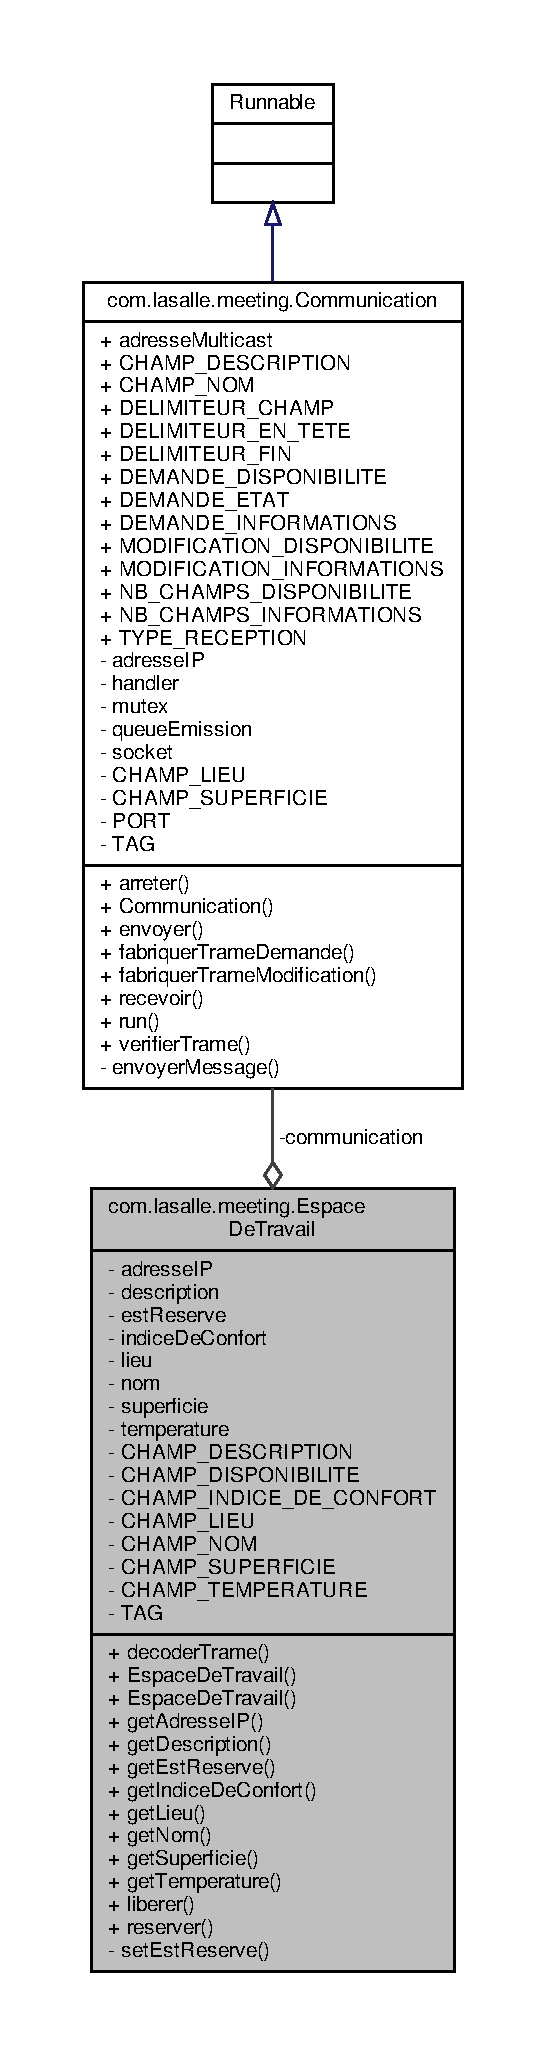
\includegraphics[height=550pt]{classcom_1_1lasalle_1_1meeting_1_1_espace_de_travail__coll__graph}
\end{center}
\end{figure}
\subsubsection*{Fonctions membres publiques}
\begin{DoxyCompactItemize}
\item 
void \hyperlink{classcom_1_1lasalle_1_1meeting_1_1_espace_de_travail_aa922390b20b7b79bcde660290f378997}{decoder\+Trame} (String trame)
\begin{DoxyCompactList}\small\item\em Décode la trame. \end{DoxyCompactList}\item 
\hyperlink{classcom_1_1lasalle_1_1meeting_1_1_espace_de_travail_a3940b7fa99249447112b00ec89fcd3d1}{Espace\+De\+Travail} ()
\begin{DoxyCompactList}\small\item\em Constructeur par défaut de la classe \hyperlink{classcom_1_1lasalle_1_1meeting_1_1_espace_de_travail}{Espace\+De\+Travail}. \end{DoxyCompactList}\item 
\hyperlink{classcom_1_1lasalle_1_1meeting_1_1_espace_de_travail_aa1f0c767a1b77048cfad17bbd49e9fe5}{Espace\+De\+Travail} (String \hyperlink{classcom_1_1lasalle_1_1meeting_1_1_espace_de_travail_aa4d9547d0170feeeb49c123e36226b79}{adresse\+IP}, String \hyperlink{classcom_1_1lasalle_1_1meeting_1_1_espace_de_travail_a9c06de6de73757cbec902e14055969ce}{nom}, String \hyperlink{classcom_1_1lasalle_1_1meeting_1_1_espace_de_travail_a375f1e6b0d3590706d863f6dbd86dd11}{lieu}, String \hyperlink{classcom_1_1lasalle_1_1meeting_1_1_espace_de_travail_a4633baf86d38c201c7e288fda3604bd7}{description}, int \hyperlink{classcom_1_1lasalle_1_1meeting_1_1_espace_de_travail_a3a5b9c42fa29930b092154e1bd0e4c10}{superficie}, int \hyperlink{classcom_1_1lasalle_1_1meeting_1_1_espace_de_travail_ad5349fa46af27855755ce6cee644a6e2}{temperature}, int \hyperlink{classcom_1_1lasalle_1_1meeting_1_1_espace_de_travail_a6a75c9c45ccb98895e02a1864bf4a41d}{indice\+De\+Confort}, boolean \hyperlink{classcom_1_1lasalle_1_1meeting_1_1_espace_de_travail_a8913c30ae6b72ae4f35962b1ecfc496b}{est\+Reserve})
\begin{DoxyCompactList}\small\item\em Constructeur de la classe \hyperlink{classcom_1_1lasalle_1_1meeting_1_1_espace_de_travail}{Espace\+De\+Travail}. \end{DoxyCompactList}\item 
String \hyperlink{classcom_1_1lasalle_1_1meeting_1_1_espace_de_travail_a24e21e44c3fc6ea5a8c68ab2cb1e22e3}{get\+Adresse\+IP} ()
\item 
String \hyperlink{classcom_1_1lasalle_1_1meeting_1_1_espace_de_travail_a815ecee3f01117f2d9b1d9441b214907}{get\+Description} ()
\item 
boolean \hyperlink{classcom_1_1lasalle_1_1meeting_1_1_espace_de_travail_a69fe30f8d3aff92986f4c39402e16ab0}{get\+Est\+Reserve} ()
\item 
int \hyperlink{classcom_1_1lasalle_1_1meeting_1_1_espace_de_travail_a9d7b3bd8aa78a10c70851b477d0f522d}{get\+Indice\+De\+Confort} ()
\item 
String \hyperlink{classcom_1_1lasalle_1_1meeting_1_1_espace_de_travail_af320aa4ad7711ed52b3b5aef1bd52dd1}{get\+Lieu} ()
\item 
String \hyperlink{classcom_1_1lasalle_1_1meeting_1_1_espace_de_travail_ae662e2674616a8548755cb64a38e0432}{get\+Nom} ()
\item 
int \hyperlink{classcom_1_1lasalle_1_1meeting_1_1_espace_de_travail_ae2c734da9d454b368ddb056b1cdae499}{get\+Superficie} ()
\item 
int \hyperlink{classcom_1_1lasalle_1_1meeting_1_1_espace_de_travail_a4c01c37fa6431d48c59274aaa00fdbe3}{get\+Temperature} ()
\item 
void \hyperlink{classcom_1_1lasalle_1_1meeting_1_1_espace_de_travail_affce017a0a5ba338d7b0b7f6bbce6c68}{liberer} ()
\begin{DoxyCompactList}\small\item\em Libère l\textquotesingle{}espace de travail. \end{DoxyCompactList}\item 
void \hyperlink{classcom_1_1lasalle_1_1meeting_1_1_espace_de_travail_a42d483a68e6d0d50707dbd3dddd164c2}{reserver} ()
\begin{DoxyCompactList}\small\item\em Réserve l\textquotesingle{}espace de travail. \end{DoxyCompactList}\end{DoxyCompactItemize}
\subsubsection*{Fonctions membres privées}
\begin{DoxyCompactItemize}
\item 
void \hyperlink{classcom_1_1lasalle_1_1meeting_1_1_espace_de_travail_ae6609cc6e5c42c0be7936ef3a3748bd0}{set\+Est\+Reserve} (boolean \hyperlink{classcom_1_1lasalle_1_1meeting_1_1_espace_de_travail_a8913c30ae6b72ae4f35962b1ecfc496b}{est\+Reserve})
\end{DoxyCompactItemize}
\subsubsection*{Attributs privés}
\begin{DoxyCompactItemize}
\item 
String \hyperlink{classcom_1_1lasalle_1_1meeting_1_1_espace_de_travail_aa4d9547d0170feeeb49c123e36226b79}{adresse\+IP}
\item 
String \hyperlink{classcom_1_1lasalle_1_1meeting_1_1_espace_de_travail_a4633baf86d38c201c7e288fda3604bd7}{description}
\item 
boolean \hyperlink{classcom_1_1lasalle_1_1meeting_1_1_espace_de_travail_a8913c30ae6b72ae4f35962b1ecfc496b}{est\+Reserve}
\item 
int \hyperlink{classcom_1_1lasalle_1_1meeting_1_1_espace_de_travail_a6a75c9c45ccb98895e02a1864bf4a41d}{indice\+De\+Confort}
\item 
String \hyperlink{classcom_1_1lasalle_1_1meeting_1_1_espace_de_travail_a375f1e6b0d3590706d863f6dbd86dd11}{lieu}
\item 
String \hyperlink{classcom_1_1lasalle_1_1meeting_1_1_espace_de_travail_a9c06de6de73757cbec902e14055969ce}{nom}
\item 
int \hyperlink{classcom_1_1lasalle_1_1meeting_1_1_espace_de_travail_a3a5b9c42fa29930b092154e1bd0e4c10}{superficie}
\item 
int \hyperlink{classcom_1_1lasalle_1_1meeting_1_1_espace_de_travail_ad5349fa46af27855755ce6cee644a6e2}{temperature}
\end{DoxyCompactItemize}
\subsubsection*{Attributs privés statiques}
\begin{DoxyCompactItemize}
\item 
static final int \hyperlink{classcom_1_1lasalle_1_1meeting_1_1_espace_de_travail_a9284e3c1fd38eae57b74ca814b285586}{C\+H\+A\+M\+P\+\_\+\+D\+E\+S\+C\+R\+I\+P\+T\+I\+ON} = 1
\item 
static final int \hyperlink{classcom_1_1lasalle_1_1meeting_1_1_espace_de_travail_a74d29b35a8171181988487a87782f26f}{C\+H\+A\+M\+P\+\_\+\+D\+I\+S\+P\+O\+N\+I\+B\+I\+L\+I\+TE} = 4
\item 
static final int \hyperlink{classcom_1_1lasalle_1_1meeting_1_1_espace_de_travail_a51854896c3a74fc72477b4fe556cd519}{C\+H\+A\+M\+P\+\_\+\+I\+N\+D\+I\+C\+E\+\_\+\+D\+E\+\_\+\+C\+O\+N\+F\+O\+RT} = 5
\item 
static final int \hyperlink{classcom_1_1lasalle_1_1meeting_1_1_espace_de_travail_aec533da6058aa1eea7c92e4f6e174f1a}{C\+H\+A\+M\+P\+\_\+\+L\+I\+EU} = 2
\item 
static final int \hyperlink{classcom_1_1lasalle_1_1meeting_1_1_espace_de_travail_a30fbba6ac01606498fbc123f1bbeaf14}{C\+H\+A\+M\+P\+\_\+\+N\+OM} = 0
\item 
static final int \hyperlink{classcom_1_1lasalle_1_1meeting_1_1_espace_de_travail_a3f0b742c19d2e62d86c7a464d326e555}{C\+H\+A\+M\+P\+\_\+\+S\+U\+P\+E\+R\+F\+I\+C\+IE} = 3
\item 
static final int \hyperlink{classcom_1_1lasalle_1_1meeting_1_1_espace_de_travail_a71c8e2beaf3f0a5584eb614e5a68bd29}{C\+H\+A\+M\+P\+\_\+\+T\+E\+M\+P\+E\+R\+A\+T\+U\+RE} = 6
\item 
static \hyperlink{classcom_1_1lasalle_1_1meeting_1_1_communication}{Communication} \hyperlink{classcom_1_1lasalle_1_1meeting_1_1_espace_de_travail_adbda10d59725486cb1151c050a830114}{communication} = null
\item 
static final String \hyperlink{classcom_1_1lasalle_1_1meeting_1_1_espace_de_travail_a30a7c9d0d084360b166487dbcdf5bad1}{T\+AG} = \char`\"{}\+\_\+\+Espace\+De\+Travail\char`\"{}
\end{DoxyCompactItemize}


\subsubsection{Description détaillée}
L\textquotesingle{}espace de travail. 

Définition à la ligne \hyperlink{_espace_de_travail_8java_source_l00021}{21} du fichier \hyperlink{_espace_de_travail_8java_source}{Espace\+De\+Travail.\+java}.



\subsubsection{Documentation des constructeurs et destructeur}
\mbox{\Hypertarget{classcom_1_1lasalle_1_1meeting_1_1_espace_de_travail_a3940b7fa99249447112b00ec89fcd3d1}\label{classcom_1_1lasalle_1_1meeting_1_1_espace_de_travail_a3940b7fa99249447112b00ec89fcd3d1}} 
\index{com\+::lasalle\+::meeting\+::\+Espace\+De\+Travail@{com\+::lasalle\+::meeting\+::\+Espace\+De\+Travail}!Espace\+De\+Travail@{Espace\+De\+Travail}}
\index{Espace\+De\+Travail@{Espace\+De\+Travail}!com\+::lasalle\+::meeting\+::\+Espace\+De\+Travail@{com\+::lasalle\+::meeting\+::\+Espace\+De\+Travail}}
\paragraph{\texorpdfstring{Espace\+De\+Travail()}{EspaceDeTravail()}\hspace{0.1cm}{\footnotesize\ttfamily [1/2]}}
{\footnotesize\ttfamily com.\+lasalle.\+meeting.\+Espace\+De\+Travail.\+Espace\+De\+Travail (\begin{DoxyParamCaption}{ }\end{DoxyParamCaption})}



Constructeur par défaut de la classe \hyperlink{classcom_1_1lasalle_1_1meeting_1_1_espace_de_travail}{Espace\+De\+Travail}. 



Définition à la ligne \hyperlink{_espace_de_travail_8java_source_l00055}{55} du fichier \hyperlink{_espace_de_travail_8java_source}{Espace\+De\+Travail.\+java}.


\begin{DoxyCode}
00056     \{
00057         this.\hyperlink{classcom_1_1lasalle_1_1meeting_1_1_espace_de_travail_aa4d9547d0170feeeb49c123e36226b79}{adresseIP} = \textcolor{stringliteral}{"\(\backslash\)0"};
00058         this.\hyperlink{classcom_1_1lasalle_1_1meeting_1_1_espace_de_travail_a9c06de6de73757cbec902e14055969ce}{nom} = \textcolor{stringliteral}{"\(\backslash\)0"};
00059         this.\hyperlink{classcom_1_1lasalle_1_1meeting_1_1_espace_de_travail_a375f1e6b0d3590706d863f6dbd86dd11}{lieu} = \textcolor{stringliteral}{"\(\backslash\)0"};
00060         this.\hyperlink{classcom_1_1lasalle_1_1meeting_1_1_espace_de_travail_a4633baf86d38c201c7e288fda3604bd7}{description} = \textcolor{stringliteral}{"\(\backslash\)0"};
00061         this.\hyperlink{classcom_1_1lasalle_1_1meeting_1_1_espace_de_travail_a3a5b9c42fa29930b092154e1bd0e4c10}{superficie} = 0;
00062         this.\hyperlink{classcom_1_1lasalle_1_1meeting_1_1_espace_de_travail_ad5349fa46af27855755ce6cee644a6e2}{temperature} = 0;
00063         this.\hyperlink{classcom_1_1lasalle_1_1meeting_1_1_espace_de_travail_a6a75c9c45ccb98895e02a1864bf4a41d}{indiceDeConfort} = 0;
00064         this.\hyperlink{classcom_1_1lasalle_1_1meeting_1_1_espace_de_travail_a8913c30ae6b72ae4f35962b1ecfc496b}{estReserve} = \textcolor{keyword}{false};
00065     \}
\end{DoxyCode}
\mbox{\Hypertarget{classcom_1_1lasalle_1_1meeting_1_1_espace_de_travail_aa1f0c767a1b77048cfad17bbd49e9fe5}\label{classcom_1_1lasalle_1_1meeting_1_1_espace_de_travail_aa1f0c767a1b77048cfad17bbd49e9fe5}} 
\index{com\+::lasalle\+::meeting\+::\+Espace\+De\+Travail@{com\+::lasalle\+::meeting\+::\+Espace\+De\+Travail}!Espace\+De\+Travail@{Espace\+De\+Travail}}
\index{Espace\+De\+Travail@{Espace\+De\+Travail}!com\+::lasalle\+::meeting\+::\+Espace\+De\+Travail@{com\+::lasalle\+::meeting\+::\+Espace\+De\+Travail}}
\paragraph{\texorpdfstring{Espace\+De\+Travail()}{EspaceDeTravail()}\hspace{0.1cm}{\footnotesize\ttfamily [2/2]}}
{\footnotesize\ttfamily com.\+lasalle.\+meeting.\+Espace\+De\+Travail.\+Espace\+De\+Travail (\begin{DoxyParamCaption}\item[{String}]{adresse\+IP,  }\item[{String}]{nom,  }\item[{String}]{lieu,  }\item[{String}]{description,  }\item[{int}]{superficie,  }\item[{int}]{temperature,  }\item[{int}]{indice\+De\+Confort,  }\item[{boolean}]{est\+Reserve }\end{DoxyParamCaption})}



Constructeur de la classe \hyperlink{classcom_1_1lasalle_1_1meeting_1_1_espace_de_travail}{Espace\+De\+Travail}. 



Définition à la ligne \hyperlink{_espace_de_travail_8java_source_l00070}{70} du fichier \hyperlink{_espace_de_travail_8java_source}{Espace\+De\+Travail.\+java}.



Références \hyperlink{_espace_de_travail_8java_source_l00031}{com.\+lasalle.\+meeting.\+Espace\+De\+Travail.\+adresse\+IP}, \hyperlink{_espace_de_travail_8java_source_l00034}{com.\+lasalle.\+meeting.\+Espace\+De\+Travail.\+description}, \hyperlink{_espace_de_travail_8java_source_l00038}{com.\+lasalle.\+meeting.\+Espace\+De\+Travail.\+est\+Reserve}, \hyperlink{_espace_de_travail_8java_source_l00037}{com.\+lasalle.\+meeting.\+Espace\+De\+Travail.\+indice\+De\+Confort}, \hyperlink{_espace_de_travail_8java_source_l00033}{com.\+lasalle.\+meeting.\+Espace\+De\+Travail.\+lieu}, \hyperlink{_espace_de_travail_8java_source_l00032}{com.\+lasalle.\+meeting.\+Espace\+De\+Travail.\+nom}, \hyperlink{_espace_de_travail_8java_source_l00035}{com.\+lasalle.\+meeting.\+Espace\+De\+Travail.\+superficie}, et \hyperlink{_espace_de_travail_8java_source_l00036}{com.\+lasalle.\+meeting.\+Espace\+De\+Travail.\+temperature}.


\begin{DoxyCode}
00071     \{
00072         this.\hyperlink{classcom_1_1lasalle_1_1meeting_1_1_espace_de_travail_aa4d9547d0170feeeb49c123e36226b79}{adresseIP} = \hyperlink{classcom_1_1lasalle_1_1meeting_1_1_espace_de_travail_aa4d9547d0170feeeb49c123e36226b79}{adresseIP};
00073         this.\hyperlink{classcom_1_1lasalle_1_1meeting_1_1_espace_de_travail_a9c06de6de73757cbec902e14055969ce}{nom} = \hyperlink{classcom_1_1lasalle_1_1meeting_1_1_espace_de_travail_a9c06de6de73757cbec902e14055969ce}{nom};
00074         this.\hyperlink{classcom_1_1lasalle_1_1meeting_1_1_espace_de_travail_a375f1e6b0d3590706d863f6dbd86dd11}{lieu} = \hyperlink{classcom_1_1lasalle_1_1meeting_1_1_espace_de_travail_a375f1e6b0d3590706d863f6dbd86dd11}{lieu};
00075         this.\hyperlink{classcom_1_1lasalle_1_1meeting_1_1_espace_de_travail_a4633baf86d38c201c7e288fda3604bd7}{description} = \hyperlink{classcom_1_1lasalle_1_1meeting_1_1_espace_de_travail_a4633baf86d38c201c7e288fda3604bd7}{description};
00076         this.\hyperlink{classcom_1_1lasalle_1_1meeting_1_1_espace_de_travail_a3a5b9c42fa29930b092154e1bd0e4c10}{superficie} = \hyperlink{classcom_1_1lasalle_1_1meeting_1_1_espace_de_travail_a3a5b9c42fa29930b092154e1bd0e4c10}{superficie};
00077         this.\hyperlink{classcom_1_1lasalle_1_1meeting_1_1_espace_de_travail_ad5349fa46af27855755ce6cee644a6e2}{temperature} = \hyperlink{classcom_1_1lasalle_1_1meeting_1_1_espace_de_travail_ad5349fa46af27855755ce6cee644a6e2}{temperature};
00078         this.\hyperlink{classcom_1_1lasalle_1_1meeting_1_1_espace_de_travail_a6a75c9c45ccb98895e02a1864bf4a41d}{indiceDeConfort} = \hyperlink{classcom_1_1lasalle_1_1meeting_1_1_espace_de_travail_a6a75c9c45ccb98895e02a1864bf4a41d}{indiceDeConfort};
00079         this.\hyperlink{classcom_1_1lasalle_1_1meeting_1_1_espace_de_travail_a8913c30ae6b72ae4f35962b1ecfc496b}{estReserve} = \hyperlink{classcom_1_1lasalle_1_1meeting_1_1_espace_de_travail_a8913c30ae6b72ae4f35962b1ecfc496b}{estReserve};
00080     \}
\end{DoxyCode}


\subsubsection{Documentation des fonctions membres}
\mbox{\Hypertarget{classcom_1_1lasalle_1_1meeting_1_1_espace_de_travail_aa922390b20b7b79bcde660290f378997}\label{classcom_1_1lasalle_1_1meeting_1_1_espace_de_travail_aa922390b20b7b79bcde660290f378997}} 
\index{com\+::lasalle\+::meeting\+::\+Espace\+De\+Travail@{com\+::lasalle\+::meeting\+::\+Espace\+De\+Travail}!decoder\+Trame@{decoder\+Trame}}
\index{decoder\+Trame@{decoder\+Trame}!com\+::lasalle\+::meeting\+::\+Espace\+De\+Travail@{com\+::lasalle\+::meeting\+::\+Espace\+De\+Travail}}
\paragraph{\texorpdfstring{decoder\+Trame()}{decoderTrame()}}
{\footnotesize\ttfamily void com.\+lasalle.\+meeting.\+Espace\+De\+Travail.\+decoder\+Trame (\begin{DoxyParamCaption}\item[{String}]{trame }\end{DoxyParamCaption})}



Décode la trame. 


\begin{DoxyParams}{Paramètres}
{\em trame} & la trame à décoder \\
\hline
\end{DoxyParams}
Protocole \+: \$nom\+Salle;description;emplacement;surface;disponibilité;niveau\+De\+Confort;température~\newline
\$nom\+Salle;disponibilité;niveau\+De\+Confort;température~\newline
\$nom\+Salle;disponibilité~\newline
 

Définition à la ligne \hyperlink{_espace_de_travail_8java_source_l00161}{161} du fichier \hyperlink{_espace_de_travail_8java_source}{Espace\+De\+Travail.\+java}.



Références \hyperlink{_espace_de_travail_8java_source_l00045}{com.\+lasalle.\+meeting.\+Espace\+De\+Travail.\+C\+H\+A\+M\+P\+\_\+\+D\+E\+S\+C\+R\+I\+P\+T\+I\+ON}, \hyperlink{_espace_de_travail_8java_source_l00046}{com.\+lasalle.\+meeting.\+Espace\+De\+Travail.\+C\+H\+A\+M\+P\+\_\+\+L\+I\+EU}, et \hyperlink{_espace_de_travail_8java_source_l00044}{com.\+lasalle.\+meeting.\+Espace\+De\+Travail.\+C\+H\+A\+M\+P\+\_\+\+N\+OM}.


\begin{DoxyCode}
00162     \{
00170         trame = trame.replace(\textcolor{stringliteral}{"$"}, \textcolor{stringliteral}{""});
00171         trame = trame.replace(\textcolor{stringliteral}{"\(\backslash\)r\(\backslash\)n"}, \textcolor{stringliteral}{""});
00172         String[] champs = trame.split(\textcolor{stringliteral}{";"});
00173 
00174         this.\hyperlink{classcom_1_1lasalle_1_1meeting_1_1_espace_de_travail_a9c06de6de73757cbec902e14055969ce}{nom} = champs[\hyperlink{classcom_1_1lasalle_1_1meeting_1_1_espace_de_travail_a30fbba6ac01606498fbc123f1bbeaf14}{CHAMP\_NOM}];
00175         this.\hyperlink{classcom_1_1lasalle_1_1meeting_1_1_espace_de_travail_a4633baf86d38c201c7e288fda3604bd7}{description} = champs[\hyperlink{classcom_1_1lasalle_1_1meeting_1_1_espace_de_travail_a9284e3c1fd38eae57b74ca814b285586}{CHAMP\_DESCRIPTION}];
00176         this.\hyperlink{classcom_1_1lasalle_1_1meeting_1_1_espace_de_travail_a375f1e6b0d3590706d863f6dbd86dd11}{lieu} = champs[\hyperlink{classcom_1_1lasalle_1_1meeting_1_1_espace_de_travail_aec533da6058aa1eea7c92e4f6e174f1a}{CHAMP\_LIEU}];
00177         this.\hyperlink{classcom_1_1lasalle_1_1meeting_1_1_espace_de_travail_a3a5b9c42fa29930b092154e1bd0e4c10}{superficie} = Integer.parseInt(champs[\hyperlink{classcom_1_1lasalle_1_1meeting_1_1_espace_de_travail_a3f0b742c19d2e62d86c7a464d326e555}{CHAMP\_SUPERFICIE}]);
00178         this.\hyperlink{classcom_1_1lasalle_1_1meeting_1_1_espace_de_travail_a8913c30ae6b72ae4f35962b1ecfc496b}{estReserve} = Boolean.parseBoolean(champs[
      \hyperlink{classcom_1_1lasalle_1_1meeting_1_1_espace_de_travail_a74d29b35a8171181988487a87782f26f}{CHAMP\_DISPONIBILITE}]);
00179         this.\hyperlink{classcom_1_1lasalle_1_1meeting_1_1_espace_de_travail_ad5349fa46af27855755ce6cee644a6e2}{temperature} = Integer.parseInt(champs[\hyperlink{classcom_1_1lasalle_1_1meeting_1_1_espace_de_travail_a71c8e2beaf3f0a5584eb614e5a68bd29}{CHAMP\_TEMPERATURE}]);
00180         this.\hyperlink{classcom_1_1lasalle_1_1meeting_1_1_espace_de_travail_a6a75c9c45ccb98895e02a1864bf4a41d}{indiceDeConfort} = Integer.parseInt(champs[
      \hyperlink{classcom_1_1lasalle_1_1meeting_1_1_espace_de_travail_a51854896c3a74fc72477b4fe556cd519}{CHAMP\_INDICE\_DE\_CONFORT}]);
00181     \}
\end{DoxyCode}
\mbox{\Hypertarget{classcom_1_1lasalle_1_1meeting_1_1_espace_de_travail_a24e21e44c3fc6ea5a8c68ab2cb1e22e3}\label{classcom_1_1lasalle_1_1meeting_1_1_espace_de_travail_a24e21e44c3fc6ea5a8c68ab2cb1e22e3}} 
\index{com\+::lasalle\+::meeting\+::\+Espace\+De\+Travail@{com\+::lasalle\+::meeting\+::\+Espace\+De\+Travail}!get\+Adresse\+IP@{get\+Adresse\+IP}}
\index{get\+Adresse\+IP@{get\+Adresse\+IP}!com\+::lasalle\+::meeting\+::\+Espace\+De\+Travail@{com\+::lasalle\+::meeting\+::\+Espace\+De\+Travail}}
\paragraph{\texorpdfstring{get\+Adresse\+I\+P()}{getAdresseIP()}}
{\footnotesize\ttfamily String com.\+lasalle.\+meeting.\+Espace\+De\+Travail.\+get\+Adresse\+IP (\begin{DoxyParamCaption}{ }\end{DoxyParamCaption})}



Définition à la ligne \hyperlink{_espace_de_travail_8java_source_l00082}{82} du fichier \hyperlink{_espace_de_travail_8java_source}{Espace\+De\+Travail.\+java}.



Références \hyperlink{_espace_de_travail_8java_source_l00031}{com.\+lasalle.\+meeting.\+Espace\+De\+Travail.\+adresse\+IP}.


\begin{DoxyCode}
00083     \{
00084         \textcolor{keywordflow}{return} \hyperlink{classcom_1_1lasalle_1_1meeting_1_1_espace_de_travail_aa4d9547d0170feeeb49c123e36226b79}{adresseIP};
00085     \}
\end{DoxyCode}
\mbox{\Hypertarget{classcom_1_1lasalle_1_1meeting_1_1_espace_de_travail_a815ecee3f01117f2d9b1d9441b214907}\label{classcom_1_1lasalle_1_1meeting_1_1_espace_de_travail_a815ecee3f01117f2d9b1d9441b214907}} 
\index{com\+::lasalle\+::meeting\+::\+Espace\+De\+Travail@{com\+::lasalle\+::meeting\+::\+Espace\+De\+Travail}!get\+Description@{get\+Description}}
\index{get\+Description@{get\+Description}!com\+::lasalle\+::meeting\+::\+Espace\+De\+Travail@{com\+::lasalle\+::meeting\+::\+Espace\+De\+Travail}}
\paragraph{\texorpdfstring{get\+Description()}{getDescription()}}
{\footnotesize\ttfamily String com.\+lasalle.\+meeting.\+Espace\+De\+Travail.\+get\+Description (\begin{DoxyParamCaption}{ }\end{DoxyParamCaption})}



Définition à la ligne \hyperlink{_espace_de_travail_8java_source_l00097}{97} du fichier \hyperlink{_espace_de_travail_8java_source}{Espace\+De\+Travail.\+java}.



Références \hyperlink{_espace_de_travail_8java_source_l00034}{com.\+lasalle.\+meeting.\+Espace\+De\+Travail.\+description}.



Référencé par \hyperlink{_affichage_espace_de_travail_8java_source_l00083}{com.\+lasalle.\+meeting.\+Affichage\+Espace\+De\+Travail.\+afficher\+Description()}, et \hyperlink{_espace_de_travail_adaptateur_8java_source_l00040}{com.\+lasalle.\+meeting.\+Espace\+De\+Travail\+Adaptateur.\+get\+View()}.


\begin{DoxyCode}
00098     \{
00099         \textcolor{keywordflow}{return} \hyperlink{classcom_1_1lasalle_1_1meeting_1_1_espace_de_travail_a4633baf86d38c201c7e288fda3604bd7}{description};
00100     \}
\end{DoxyCode}
\mbox{\Hypertarget{classcom_1_1lasalle_1_1meeting_1_1_espace_de_travail_a69fe30f8d3aff92986f4c39402e16ab0}\label{classcom_1_1lasalle_1_1meeting_1_1_espace_de_travail_a69fe30f8d3aff92986f4c39402e16ab0}} 
\index{com\+::lasalle\+::meeting\+::\+Espace\+De\+Travail@{com\+::lasalle\+::meeting\+::\+Espace\+De\+Travail}!get\+Est\+Reserve@{get\+Est\+Reserve}}
\index{get\+Est\+Reserve@{get\+Est\+Reserve}!com\+::lasalle\+::meeting\+::\+Espace\+De\+Travail@{com\+::lasalle\+::meeting\+::\+Espace\+De\+Travail}}
\paragraph{\texorpdfstring{get\+Est\+Reserve()}{getEstReserve()}}
{\footnotesize\ttfamily boolean com.\+lasalle.\+meeting.\+Espace\+De\+Travail.\+get\+Est\+Reserve (\begin{DoxyParamCaption}{ }\end{DoxyParamCaption})}



Définition à la ligne \hyperlink{_espace_de_travail_8java_source_l00117}{117} du fichier \hyperlink{_espace_de_travail_8java_source}{Espace\+De\+Travail.\+java}.



Références \hyperlink{_espace_de_travail_8java_source_l00038}{com.\+lasalle.\+meeting.\+Espace\+De\+Travail.\+est\+Reserve}.



Référencé par \hyperlink{_affichage_espace_de_travail_8java_source_l00150}{com.\+lasalle.\+meeting.\+Affichage\+Espace\+De\+Travail.\+afficher\+Boutons\+Reservation()}, \hyperlink{_affichage_espace_de_travail_8java_source_l00127}{com.\+lasalle.\+meeting.\+Affichage\+Espace\+De\+Travail.\+afficher\+Disponibilite()}, \hyperlink{_espace_de_travail_adaptateur_8java_source_l00040}{com.\+lasalle.\+meeting.\+Espace\+De\+Travail\+Adaptateur.\+get\+View()}, \hyperlink{_espace_de_travail_8java_source_l00145}{com.\+lasalle.\+meeting.\+Espace\+De\+Travail.\+liberer()}, \hyperlink{_i_h_m_meeting_8java_source_l00297}{com.\+lasalle.\+meeting.\+I\+H\+M\+Meeting.\+on\+Activity\+Result()}, et \hyperlink{_espace_de_travail_8java_source_l00130}{com.\+lasalle.\+meeting.\+Espace\+De\+Travail.\+reserver()}.


\begin{DoxyCode}
00118     \{
00119         \textcolor{keywordflow}{return} \hyperlink{classcom_1_1lasalle_1_1meeting_1_1_espace_de_travail_a8913c30ae6b72ae4f35962b1ecfc496b}{estReserve};
00120     \}
\end{DoxyCode}
\mbox{\Hypertarget{classcom_1_1lasalle_1_1meeting_1_1_espace_de_travail_a9d7b3bd8aa78a10c70851b477d0f522d}\label{classcom_1_1lasalle_1_1meeting_1_1_espace_de_travail_a9d7b3bd8aa78a10c70851b477d0f522d}} 
\index{com\+::lasalle\+::meeting\+::\+Espace\+De\+Travail@{com\+::lasalle\+::meeting\+::\+Espace\+De\+Travail}!get\+Indice\+De\+Confort@{get\+Indice\+De\+Confort}}
\index{get\+Indice\+De\+Confort@{get\+Indice\+De\+Confort}!com\+::lasalle\+::meeting\+::\+Espace\+De\+Travail@{com\+::lasalle\+::meeting\+::\+Espace\+De\+Travail}}
\paragraph{\texorpdfstring{get\+Indice\+De\+Confort()}{getIndiceDeConfort()}}
{\footnotesize\ttfamily int com.\+lasalle.\+meeting.\+Espace\+De\+Travail.\+get\+Indice\+De\+Confort (\begin{DoxyParamCaption}{ }\end{DoxyParamCaption})}



Définition à la ligne \hyperlink{_espace_de_travail_8java_source_l00112}{112} du fichier \hyperlink{_espace_de_travail_8java_source}{Espace\+De\+Travail.\+java}.



Références \hyperlink{_espace_de_travail_8java_source_l00037}{com.\+lasalle.\+meeting.\+Espace\+De\+Travail.\+indice\+De\+Confort}.



Référencé par \hyperlink{_affichage_espace_de_travail_8java_source_l00116}{com.\+lasalle.\+meeting.\+Affichage\+Espace\+De\+Travail.\+afficher\+Indice\+De\+Confort()}.


\begin{DoxyCode}
00113     \{
00114         \textcolor{keywordflow}{return} \hyperlink{classcom_1_1lasalle_1_1meeting_1_1_espace_de_travail_a6a75c9c45ccb98895e02a1864bf4a41d}{indiceDeConfort};
00115     \}
\end{DoxyCode}
\mbox{\Hypertarget{classcom_1_1lasalle_1_1meeting_1_1_espace_de_travail_af320aa4ad7711ed52b3b5aef1bd52dd1}\label{classcom_1_1lasalle_1_1meeting_1_1_espace_de_travail_af320aa4ad7711ed52b3b5aef1bd52dd1}} 
\index{com\+::lasalle\+::meeting\+::\+Espace\+De\+Travail@{com\+::lasalle\+::meeting\+::\+Espace\+De\+Travail}!get\+Lieu@{get\+Lieu}}
\index{get\+Lieu@{get\+Lieu}!com\+::lasalle\+::meeting\+::\+Espace\+De\+Travail@{com\+::lasalle\+::meeting\+::\+Espace\+De\+Travail}}
\paragraph{\texorpdfstring{get\+Lieu()}{getLieu()}}
{\footnotesize\ttfamily String com.\+lasalle.\+meeting.\+Espace\+De\+Travail.\+get\+Lieu (\begin{DoxyParamCaption}{ }\end{DoxyParamCaption})}



Définition à la ligne \hyperlink{_espace_de_travail_8java_source_l00092}{92} du fichier \hyperlink{_espace_de_travail_8java_source}{Espace\+De\+Travail.\+java}.



Références \hyperlink{_espace_de_travail_8java_source_l00033}{com.\+lasalle.\+meeting.\+Espace\+De\+Travail.\+lieu}.



Référencé par \hyperlink{_affichage_espace_de_travail_8java_source_l00072}{com.\+lasalle.\+meeting.\+Affichage\+Espace\+De\+Travail.\+afficher\+Lieu()}.


\begin{DoxyCode}
00093     \{
00094         \textcolor{keywordflow}{return} \hyperlink{classcom_1_1lasalle_1_1meeting_1_1_espace_de_travail_a375f1e6b0d3590706d863f6dbd86dd11}{lieu};
00095     \}
\end{DoxyCode}
\mbox{\Hypertarget{classcom_1_1lasalle_1_1meeting_1_1_espace_de_travail_ae662e2674616a8548755cb64a38e0432}\label{classcom_1_1lasalle_1_1meeting_1_1_espace_de_travail_ae662e2674616a8548755cb64a38e0432}} 
\index{com\+::lasalle\+::meeting\+::\+Espace\+De\+Travail@{com\+::lasalle\+::meeting\+::\+Espace\+De\+Travail}!get\+Nom@{get\+Nom}}
\index{get\+Nom@{get\+Nom}!com\+::lasalle\+::meeting\+::\+Espace\+De\+Travail@{com\+::lasalle\+::meeting\+::\+Espace\+De\+Travail}}
\paragraph{\texorpdfstring{get\+Nom()}{getNom()}}
{\footnotesize\ttfamily String com.\+lasalle.\+meeting.\+Espace\+De\+Travail.\+get\+Nom (\begin{DoxyParamCaption}{ }\end{DoxyParamCaption})}



Définition à la ligne \hyperlink{_espace_de_travail_8java_source_l00087}{87} du fichier \hyperlink{_espace_de_travail_8java_source}{Espace\+De\+Travail.\+java}.



Références \hyperlink{_espace_de_travail_8java_source_l00032}{com.\+lasalle.\+meeting.\+Espace\+De\+Travail.\+nom}.



Référencé par \hyperlink{_affichage_espace_de_travail_8java_source_l00061}{com.\+lasalle.\+meeting.\+Affichage\+Espace\+De\+Travail.\+afficher\+Nom()}, \hyperlink{_espace_de_travail_adaptateur_8java_source_l00040}{com.\+lasalle.\+meeting.\+Espace\+De\+Travail\+Adaptateur.\+get\+View()}, et \hyperlink{_i_h_m_meeting_8java_source_l00248}{com.\+lasalle.\+meeting.\+I\+H\+M\+Meeting.\+verifier\+Presence\+Espace\+De\+Travail()}.


\begin{DoxyCode}
00088     \{
00089         \textcolor{keywordflow}{return} \hyperlink{classcom_1_1lasalle_1_1meeting_1_1_espace_de_travail_a9c06de6de73757cbec902e14055969ce}{nom};
00090     \}
\end{DoxyCode}
\mbox{\Hypertarget{classcom_1_1lasalle_1_1meeting_1_1_espace_de_travail_ae2c734da9d454b368ddb056b1cdae499}\label{classcom_1_1lasalle_1_1meeting_1_1_espace_de_travail_ae2c734da9d454b368ddb056b1cdae499}} 
\index{com\+::lasalle\+::meeting\+::\+Espace\+De\+Travail@{com\+::lasalle\+::meeting\+::\+Espace\+De\+Travail}!get\+Superficie@{get\+Superficie}}
\index{get\+Superficie@{get\+Superficie}!com\+::lasalle\+::meeting\+::\+Espace\+De\+Travail@{com\+::lasalle\+::meeting\+::\+Espace\+De\+Travail}}
\paragraph{\texorpdfstring{get\+Superficie()}{getSuperficie()}}
{\footnotesize\ttfamily int com.\+lasalle.\+meeting.\+Espace\+De\+Travail.\+get\+Superficie (\begin{DoxyParamCaption}{ }\end{DoxyParamCaption})}



Définition à la ligne \hyperlink{_espace_de_travail_8java_source_l00102}{102} du fichier \hyperlink{_espace_de_travail_8java_source}{Espace\+De\+Travail.\+java}.



Références \hyperlink{_espace_de_travail_8java_source_l00035}{com.\+lasalle.\+meeting.\+Espace\+De\+Travail.\+superficie}.



Référencé par \hyperlink{_affichage_espace_de_travail_8java_source_l00094}{com.\+lasalle.\+meeting.\+Affichage\+Espace\+De\+Travail.\+afficher\+Superficie()}.


\begin{DoxyCode}
00103     \{
00104         \textcolor{keywordflow}{return} \hyperlink{classcom_1_1lasalle_1_1meeting_1_1_espace_de_travail_a3a5b9c42fa29930b092154e1bd0e4c10}{superficie};
00105     \}
\end{DoxyCode}
\mbox{\Hypertarget{classcom_1_1lasalle_1_1meeting_1_1_espace_de_travail_a4c01c37fa6431d48c59274aaa00fdbe3}\label{classcom_1_1lasalle_1_1meeting_1_1_espace_de_travail_a4c01c37fa6431d48c59274aaa00fdbe3}} 
\index{com\+::lasalle\+::meeting\+::\+Espace\+De\+Travail@{com\+::lasalle\+::meeting\+::\+Espace\+De\+Travail}!get\+Temperature@{get\+Temperature}}
\index{get\+Temperature@{get\+Temperature}!com\+::lasalle\+::meeting\+::\+Espace\+De\+Travail@{com\+::lasalle\+::meeting\+::\+Espace\+De\+Travail}}
\paragraph{\texorpdfstring{get\+Temperature()}{getTemperature()}}
{\footnotesize\ttfamily int com.\+lasalle.\+meeting.\+Espace\+De\+Travail.\+get\+Temperature (\begin{DoxyParamCaption}{ }\end{DoxyParamCaption})}



Définition à la ligne \hyperlink{_espace_de_travail_8java_source_l00107}{107} du fichier \hyperlink{_espace_de_travail_8java_source}{Espace\+De\+Travail.\+java}.



Références \hyperlink{_espace_de_travail_8java_source_l00036}{com.\+lasalle.\+meeting.\+Espace\+De\+Travail.\+temperature}.



Référencé par \hyperlink{_affichage_espace_de_travail_8java_source_l00105}{com.\+lasalle.\+meeting.\+Affichage\+Espace\+De\+Travail.\+afficher\+Temperature()}.


\begin{DoxyCode}
00108     \{
00109         \textcolor{keywordflow}{return} \hyperlink{classcom_1_1lasalle_1_1meeting_1_1_espace_de_travail_ad5349fa46af27855755ce6cee644a6e2}{temperature};
00110     \}
\end{DoxyCode}
\mbox{\Hypertarget{classcom_1_1lasalle_1_1meeting_1_1_espace_de_travail_affce017a0a5ba338d7b0b7f6bbce6c68}\label{classcom_1_1lasalle_1_1meeting_1_1_espace_de_travail_affce017a0a5ba338d7b0b7f6bbce6c68}} 
\index{com\+::lasalle\+::meeting\+::\+Espace\+De\+Travail@{com\+::lasalle\+::meeting\+::\+Espace\+De\+Travail}!liberer@{liberer}}
\index{liberer@{liberer}!com\+::lasalle\+::meeting\+::\+Espace\+De\+Travail@{com\+::lasalle\+::meeting\+::\+Espace\+De\+Travail}}
\paragraph{\texorpdfstring{liberer()}{liberer()}}
{\footnotesize\ttfamily void com.\+lasalle.\+meeting.\+Espace\+De\+Travail.\+liberer (\begin{DoxyParamCaption}{ }\end{DoxyParamCaption})}



Libère l\textquotesingle{}espace de travail. 



Définition à la ligne \hyperlink{_espace_de_travail_8java_source_l00145}{145} du fichier \hyperlink{_espace_de_travail_8java_source}{Espace\+De\+Travail.\+java}.



Références \hyperlink{_communication_8java_source_l00222}{com.\+lasalle.\+meeting.\+Communication.\+fabriquer\+Trame\+Modification()}, \hyperlink{_espace_de_travail_8java_source_l00117}{com.\+lasalle.\+meeting.\+Espace\+De\+Travail.\+get\+Est\+Reserve()}, \hyperlink{_communication_8java_source_l00058}{com.\+lasalle.\+meeting.\+Communication.\+M\+O\+D\+I\+F\+I\+C\+A\+T\+I\+O\+N\+\_\+\+D\+I\+S\+P\+O\+N\+I\+B\+I\+L\+I\+TE}, et \hyperlink{_espace_de_travail_8java_source_l00122}{com.\+lasalle.\+meeting.\+Espace\+De\+Travail.\+set\+Est\+Reserve()}.



Référencé par \hyperlink{_affichage_espace_de_travail_8java_source_l00150}{com.\+lasalle.\+meeting.\+Affichage\+Espace\+De\+Travail.\+afficher\+Boutons\+Reservation()}.


\begin{DoxyCode}
00146     \{
00147         Log.d(\hyperlink{classcom_1_1lasalle_1_1meeting_1_1_espace_de_travail_a30a7c9d0d084360b166487dbcdf5bad1}{TAG}, \textcolor{stringliteral}{"liberer()"});
00148 
00149         List<String> parametres = Arrays.asList(String.valueOf(\textcolor{keyword}{false}));
00150         \hyperlink{classcom_1_1lasalle_1_1meeting_1_1_espace_de_travail_adbda10d59725486cb1151c050a830114}{communication}.\hyperlink{classcom_1_1lasalle_1_1meeting_1_1_communication_a82b49090e24d8296bfd26a14e0951ade}{fabriquerTrameModification}(Communication.
      MODIFICATION\_DISPONIBILITE, parametres);
00151 
00152         \hyperlink{classcom_1_1lasalle_1_1meeting_1_1_espace_de_travail_ae6609cc6e5c42c0be7936ef3a3748bd0}{setEstReserve}(\textcolor{keyword}{false});
00153 
00154         Log.d(\hyperlink{classcom_1_1lasalle_1_1meeting_1_1_espace_de_travail_a30a7c9d0d084360b166487dbcdf5bad1}{TAG}, \textcolor{stringliteral}{"getEstReserve() "} + \hyperlink{classcom_1_1lasalle_1_1meeting_1_1_espace_de_travail_a69fe30f8d3aff92986f4c39402e16ab0}{getEstReserve}());
00155     \}
\end{DoxyCode}
\mbox{\Hypertarget{classcom_1_1lasalle_1_1meeting_1_1_espace_de_travail_a42d483a68e6d0d50707dbd3dddd164c2}\label{classcom_1_1lasalle_1_1meeting_1_1_espace_de_travail_a42d483a68e6d0d50707dbd3dddd164c2}} 
\index{com\+::lasalle\+::meeting\+::\+Espace\+De\+Travail@{com\+::lasalle\+::meeting\+::\+Espace\+De\+Travail}!reserver@{reserver}}
\index{reserver@{reserver}!com\+::lasalle\+::meeting\+::\+Espace\+De\+Travail@{com\+::lasalle\+::meeting\+::\+Espace\+De\+Travail}}
\paragraph{\texorpdfstring{reserver()}{reserver()}}
{\footnotesize\ttfamily void com.\+lasalle.\+meeting.\+Espace\+De\+Travail.\+reserver (\begin{DoxyParamCaption}{ }\end{DoxyParamCaption})}



Réserve l\textquotesingle{}espace de travail. 



Définition à la ligne \hyperlink{_espace_de_travail_8java_source_l00130}{130} du fichier \hyperlink{_espace_de_travail_8java_source}{Espace\+De\+Travail.\+java}.



Références \hyperlink{_communication_8java_source_l00222}{com.\+lasalle.\+meeting.\+Communication.\+fabriquer\+Trame\+Modification()}, \hyperlink{_espace_de_travail_8java_source_l00117}{com.\+lasalle.\+meeting.\+Espace\+De\+Travail.\+get\+Est\+Reserve()}, \hyperlink{_communication_8java_source_l00058}{com.\+lasalle.\+meeting.\+Communication.\+M\+O\+D\+I\+F\+I\+C\+A\+T\+I\+O\+N\+\_\+\+D\+I\+S\+P\+O\+N\+I\+B\+I\+L\+I\+TE}, et \hyperlink{_espace_de_travail_8java_source_l00122}{com.\+lasalle.\+meeting.\+Espace\+De\+Travail.\+set\+Est\+Reserve()}.



Référencé par \hyperlink{_affichage_espace_de_travail_8java_source_l00150}{com.\+lasalle.\+meeting.\+Affichage\+Espace\+De\+Travail.\+afficher\+Boutons\+Reservation()}.


\begin{DoxyCode}
00131     \{
00132         Log.d(\hyperlink{classcom_1_1lasalle_1_1meeting_1_1_espace_de_travail_a30a7c9d0d084360b166487dbcdf5bad1}{TAG}, \textcolor{stringliteral}{"reserver()"});
00133 
00134         List<String> parametres = Arrays.asList(String.valueOf(\textcolor{keyword}{true}));
00135         \hyperlink{classcom_1_1lasalle_1_1meeting_1_1_espace_de_travail_adbda10d59725486cb1151c050a830114}{communication}.\hyperlink{classcom_1_1lasalle_1_1meeting_1_1_communication_a82b49090e24d8296bfd26a14e0951ade}{fabriquerTrameModification}(Communication.
      MODIFICATION\_DISPONIBILITE, parametres);
00136 
00137         \hyperlink{classcom_1_1lasalle_1_1meeting_1_1_espace_de_travail_ae6609cc6e5c42c0be7936ef3a3748bd0}{setEstReserve}(\textcolor{keyword}{true});
00138 
00139         Log.d(\hyperlink{classcom_1_1lasalle_1_1meeting_1_1_espace_de_travail_a30a7c9d0d084360b166487dbcdf5bad1}{TAG}, \textcolor{stringliteral}{"getEstReserve() "} + \hyperlink{classcom_1_1lasalle_1_1meeting_1_1_espace_de_travail_a69fe30f8d3aff92986f4c39402e16ab0}{getEstReserve}());
00140     \}
\end{DoxyCode}
\mbox{\Hypertarget{classcom_1_1lasalle_1_1meeting_1_1_espace_de_travail_ae6609cc6e5c42c0be7936ef3a3748bd0}\label{classcom_1_1lasalle_1_1meeting_1_1_espace_de_travail_ae6609cc6e5c42c0be7936ef3a3748bd0}} 
\index{com\+::lasalle\+::meeting\+::\+Espace\+De\+Travail@{com\+::lasalle\+::meeting\+::\+Espace\+De\+Travail}!set\+Est\+Reserve@{set\+Est\+Reserve}}
\index{set\+Est\+Reserve@{set\+Est\+Reserve}!com\+::lasalle\+::meeting\+::\+Espace\+De\+Travail@{com\+::lasalle\+::meeting\+::\+Espace\+De\+Travail}}
\paragraph{\texorpdfstring{set\+Est\+Reserve()}{setEstReserve()}}
{\footnotesize\ttfamily void com.\+lasalle.\+meeting.\+Espace\+De\+Travail.\+set\+Est\+Reserve (\begin{DoxyParamCaption}\item[{boolean}]{est\+Reserve }\end{DoxyParamCaption})\hspace{0.3cm}{\ttfamily [private]}}



Définition à la ligne \hyperlink{_espace_de_travail_8java_source_l00122}{122} du fichier \hyperlink{_espace_de_travail_8java_source}{Espace\+De\+Travail.\+java}.



Références \hyperlink{_espace_de_travail_8java_source_l00038}{com.\+lasalle.\+meeting.\+Espace\+De\+Travail.\+est\+Reserve}.



Référencé par \hyperlink{_espace_de_travail_8java_source_l00145}{com.\+lasalle.\+meeting.\+Espace\+De\+Travail.\+liberer()}, et \hyperlink{_espace_de_travail_8java_source_l00130}{com.\+lasalle.\+meeting.\+Espace\+De\+Travail.\+reserver()}.


\begin{DoxyCode}
00123     \{
00124         this.\hyperlink{classcom_1_1lasalle_1_1meeting_1_1_espace_de_travail_a8913c30ae6b72ae4f35962b1ecfc496b}{estReserve} = \hyperlink{classcom_1_1lasalle_1_1meeting_1_1_espace_de_travail_a8913c30ae6b72ae4f35962b1ecfc496b}{estReserve};
00125     \}
\end{DoxyCode}


\subsubsection{Documentation des données membres}
\mbox{\Hypertarget{classcom_1_1lasalle_1_1meeting_1_1_espace_de_travail_aa4d9547d0170feeeb49c123e36226b79}\label{classcom_1_1lasalle_1_1meeting_1_1_espace_de_travail_aa4d9547d0170feeeb49c123e36226b79}} 
\index{com\+::lasalle\+::meeting\+::\+Espace\+De\+Travail@{com\+::lasalle\+::meeting\+::\+Espace\+De\+Travail}!adresse\+IP@{adresse\+IP}}
\index{adresse\+IP@{adresse\+IP}!com\+::lasalle\+::meeting\+::\+Espace\+De\+Travail@{com\+::lasalle\+::meeting\+::\+Espace\+De\+Travail}}
\paragraph{\texorpdfstring{adresse\+IP}{adresseIP}}
{\footnotesize\ttfamily String com.\+lasalle.\+meeting.\+Espace\+De\+Travail.\+adresse\+IP\hspace{0.3cm}{\ttfamily [private]}}

Les attributs 

Définition à la ligne \hyperlink{_espace_de_travail_8java_source_l00031}{31} du fichier \hyperlink{_espace_de_travail_8java_source}{Espace\+De\+Travail.\+java}.



Référencé par \hyperlink{_espace_de_travail_8java_source_l00070}{com.\+lasalle.\+meeting.\+Espace\+De\+Travail.\+Espace\+De\+Travail()}, et \hyperlink{_espace_de_travail_8java_source_l00082}{com.\+lasalle.\+meeting.\+Espace\+De\+Travail.\+get\+Adresse\+I\+P()}.

\mbox{\Hypertarget{classcom_1_1lasalle_1_1meeting_1_1_espace_de_travail_a9284e3c1fd38eae57b74ca814b285586}\label{classcom_1_1lasalle_1_1meeting_1_1_espace_de_travail_a9284e3c1fd38eae57b74ca814b285586}} 
\index{com\+::lasalle\+::meeting\+::\+Espace\+De\+Travail@{com\+::lasalle\+::meeting\+::\+Espace\+De\+Travail}!C\+H\+A\+M\+P\+\_\+\+D\+E\+S\+C\+R\+I\+P\+T\+I\+ON@{C\+H\+A\+M\+P\+\_\+\+D\+E\+S\+C\+R\+I\+P\+T\+I\+ON}}
\index{C\+H\+A\+M\+P\+\_\+\+D\+E\+S\+C\+R\+I\+P\+T\+I\+ON@{C\+H\+A\+M\+P\+\_\+\+D\+E\+S\+C\+R\+I\+P\+T\+I\+ON}!com\+::lasalle\+::meeting\+::\+Espace\+De\+Travail@{com\+::lasalle\+::meeting\+::\+Espace\+De\+Travail}}
\paragraph{\texorpdfstring{C\+H\+A\+M\+P\+\_\+\+D\+E\+S\+C\+R\+I\+P\+T\+I\+ON}{CHAMP\_DESCRIPTION}}
{\footnotesize\ttfamily final int com.\+lasalle.\+meeting.\+Espace\+De\+Travail.\+C\+H\+A\+M\+P\+\_\+\+D\+E\+S\+C\+R\+I\+P\+T\+I\+ON = 1\hspace{0.3cm}{\ttfamily [static]}, {\ttfamily [private]}}



Définition à la ligne \hyperlink{_espace_de_travail_8java_source_l00045}{45} du fichier \hyperlink{_espace_de_travail_8java_source}{Espace\+De\+Travail.\+java}.



Référencé par \hyperlink{_espace_de_travail_8java_source_l00161}{com.\+lasalle.\+meeting.\+Espace\+De\+Travail.\+decoder\+Trame()}.

\mbox{\Hypertarget{classcom_1_1lasalle_1_1meeting_1_1_espace_de_travail_a74d29b35a8171181988487a87782f26f}\label{classcom_1_1lasalle_1_1meeting_1_1_espace_de_travail_a74d29b35a8171181988487a87782f26f}} 
\index{com\+::lasalle\+::meeting\+::\+Espace\+De\+Travail@{com\+::lasalle\+::meeting\+::\+Espace\+De\+Travail}!C\+H\+A\+M\+P\+\_\+\+D\+I\+S\+P\+O\+N\+I\+B\+I\+L\+I\+TE@{C\+H\+A\+M\+P\+\_\+\+D\+I\+S\+P\+O\+N\+I\+B\+I\+L\+I\+TE}}
\index{C\+H\+A\+M\+P\+\_\+\+D\+I\+S\+P\+O\+N\+I\+B\+I\+L\+I\+TE@{C\+H\+A\+M\+P\+\_\+\+D\+I\+S\+P\+O\+N\+I\+B\+I\+L\+I\+TE}!com\+::lasalle\+::meeting\+::\+Espace\+De\+Travail@{com\+::lasalle\+::meeting\+::\+Espace\+De\+Travail}}
\paragraph{\texorpdfstring{C\+H\+A\+M\+P\+\_\+\+D\+I\+S\+P\+O\+N\+I\+B\+I\+L\+I\+TE}{CHAMP\_DISPONIBILITE}}
{\footnotesize\ttfamily final int com.\+lasalle.\+meeting.\+Espace\+De\+Travail.\+C\+H\+A\+M\+P\+\_\+\+D\+I\+S\+P\+O\+N\+I\+B\+I\+L\+I\+TE = 4\hspace{0.3cm}{\ttfamily [static]}, {\ttfamily [private]}}



Définition à la ligne \hyperlink{_espace_de_travail_8java_source_l00048}{48} du fichier \hyperlink{_espace_de_travail_8java_source}{Espace\+De\+Travail.\+java}.

\mbox{\Hypertarget{classcom_1_1lasalle_1_1meeting_1_1_espace_de_travail_a51854896c3a74fc72477b4fe556cd519}\label{classcom_1_1lasalle_1_1meeting_1_1_espace_de_travail_a51854896c3a74fc72477b4fe556cd519}} 
\index{com\+::lasalle\+::meeting\+::\+Espace\+De\+Travail@{com\+::lasalle\+::meeting\+::\+Espace\+De\+Travail}!C\+H\+A\+M\+P\+\_\+\+I\+N\+D\+I\+C\+E\+\_\+\+D\+E\+\_\+\+C\+O\+N\+F\+O\+RT@{C\+H\+A\+M\+P\+\_\+\+I\+N\+D\+I\+C\+E\+\_\+\+D\+E\+\_\+\+C\+O\+N\+F\+O\+RT}}
\index{C\+H\+A\+M\+P\+\_\+\+I\+N\+D\+I\+C\+E\+\_\+\+D\+E\+\_\+\+C\+O\+N\+F\+O\+RT@{C\+H\+A\+M\+P\+\_\+\+I\+N\+D\+I\+C\+E\+\_\+\+D\+E\+\_\+\+C\+O\+N\+F\+O\+RT}!com\+::lasalle\+::meeting\+::\+Espace\+De\+Travail@{com\+::lasalle\+::meeting\+::\+Espace\+De\+Travail}}
\paragraph{\texorpdfstring{C\+H\+A\+M\+P\+\_\+\+I\+N\+D\+I\+C\+E\+\_\+\+D\+E\+\_\+\+C\+O\+N\+F\+O\+RT}{CHAMP\_INDICE\_DE\_CONFORT}}
{\footnotesize\ttfamily final int com.\+lasalle.\+meeting.\+Espace\+De\+Travail.\+C\+H\+A\+M\+P\+\_\+\+I\+N\+D\+I\+C\+E\+\_\+\+D\+E\+\_\+\+C\+O\+N\+F\+O\+RT = 5\hspace{0.3cm}{\ttfamily [static]}, {\ttfamily [private]}}



Définition à la ligne \hyperlink{_espace_de_travail_8java_source_l00049}{49} du fichier \hyperlink{_espace_de_travail_8java_source}{Espace\+De\+Travail.\+java}.

\mbox{\Hypertarget{classcom_1_1lasalle_1_1meeting_1_1_espace_de_travail_aec533da6058aa1eea7c92e4f6e174f1a}\label{classcom_1_1lasalle_1_1meeting_1_1_espace_de_travail_aec533da6058aa1eea7c92e4f6e174f1a}} 
\index{com\+::lasalle\+::meeting\+::\+Espace\+De\+Travail@{com\+::lasalle\+::meeting\+::\+Espace\+De\+Travail}!C\+H\+A\+M\+P\+\_\+\+L\+I\+EU@{C\+H\+A\+M\+P\+\_\+\+L\+I\+EU}}
\index{C\+H\+A\+M\+P\+\_\+\+L\+I\+EU@{C\+H\+A\+M\+P\+\_\+\+L\+I\+EU}!com\+::lasalle\+::meeting\+::\+Espace\+De\+Travail@{com\+::lasalle\+::meeting\+::\+Espace\+De\+Travail}}
\paragraph{\texorpdfstring{C\+H\+A\+M\+P\+\_\+\+L\+I\+EU}{CHAMP\_LIEU}}
{\footnotesize\ttfamily final int com.\+lasalle.\+meeting.\+Espace\+De\+Travail.\+C\+H\+A\+M\+P\+\_\+\+L\+I\+EU = 2\hspace{0.3cm}{\ttfamily [static]}, {\ttfamily [private]}}



Définition à la ligne \hyperlink{_espace_de_travail_8java_source_l00046}{46} du fichier \hyperlink{_espace_de_travail_8java_source}{Espace\+De\+Travail.\+java}.



Référencé par \hyperlink{_espace_de_travail_8java_source_l00161}{com.\+lasalle.\+meeting.\+Espace\+De\+Travail.\+decoder\+Trame()}.

\mbox{\Hypertarget{classcom_1_1lasalle_1_1meeting_1_1_espace_de_travail_a30fbba6ac01606498fbc123f1bbeaf14}\label{classcom_1_1lasalle_1_1meeting_1_1_espace_de_travail_a30fbba6ac01606498fbc123f1bbeaf14}} 
\index{com\+::lasalle\+::meeting\+::\+Espace\+De\+Travail@{com\+::lasalle\+::meeting\+::\+Espace\+De\+Travail}!C\+H\+A\+M\+P\+\_\+\+N\+OM@{C\+H\+A\+M\+P\+\_\+\+N\+OM}}
\index{C\+H\+A\+M\+P\+\_\+\+N\+OM@{C\+H\+A\+M\+P\+\_\+\+N\+OM}!com\+::lasalle\+::meeting\+::\+Espace\+De\+Travail@{com\+::lasalle\+::meeting\+::\+Espace\+De\+Travail}}
\paragraph{\texorpdfstring{C\+H\+A\+M\+P\+\_\+\+N\+OM}{CHAMP\_NOM}}
{\footnotesize\ttfamily final int com.\+lasalle.\+meeting.\+Espace\+De\+Travail.\+C\+H\+A\+M\+P\+\_\+\+N\+OM = 0\hspace{0.3cm}{\ttfamily [static]}, {\ttfamily [private]}}

Protocole 

Définition à la ligne \hyperlink{_espace_de_travail_8java_source_l00044}{44} du fichier \hyperlink{_espace_de_travail_8java_source}{Espace\+De\+Travail.\+java}.



Référencé par \hyperlink{_espace_de_travail_8java_source_l00161}{com.\+lasalle.\+meeting.\+Espace\+De\+Travail.\+decoder\+Trame()}.

\mbox{\Hypertarget{classcom_1_1lasalle_1_1meeting_1_1_espace_de_travail_a3f0b742c19d2e62d86c7a464d326e555}\label{classcom_1_1lasalle_1_1meeting_1_1_espace_de_travail_a3f0b742c19d2e62d86c7a464d326e555}} 
\index{com\+::lasalle\+::meeting\+::\+Espace\+De\+Travail@{com\+::lasalle\+::meeting\+::\+Espace\+De\+Travail}!C\+H\+A\+M\+P\+\_\+\+S\+U\+P\+E\+R\+F\+I\+C\+IE@{C\+H\+A\+M\+P\+\_\+\+S\+U\+P\+E\+R\+F\+I\+C\+IE}}
\index{C\+H\+A\+M\+P\+\_\+\+S\+U\+P\+E\+R\+F\+I\+C\+IE@{C\+H\+A\+M\+P\+\_\+\+S\+U\+P\+E\+R\+F\+I\+C\+IE}!com\+::lasalle\+::meeting\+::\+Espace\+De\+Travail@{com\+::lasalle\+::meeting\+::\+Espace\+De\+Travail}}
\paragraph{\texorpdfstring{C\+H\+A\+M\+P\+\_\+\+S\+U\+P\+E\+R\+F\+I\+C\+IE}{CHAMP\_SUPERFICIE}}
{\footnotesize\ttfamily final int com.\+lasalle.\+meeting.\+Espace\+De\+Travail.\+C\+H\+A\+M\+P\+\_\+\+S\+U\+P\+E\+R\+F\+I\+C\+IE = 3\hspace{0.3cm}{\ttfamily [static]}, {\ttfamily [private]}}



Définition à la ligne \hyperlink{_espace_de_travail_8java_source_l00047}{47} du fichier \hyperlink{_espace_de_travail_8java_source}{Espace\+De\+Travail.\+java}.

\mbox{\Hypertarget{classcom_1_1lasalle_1_1meeting_1_1_espace_de_travail_a71c8e2beaf3f0a5584eb614e5a68bd29}\label{classcom_1_1lasalle_1_1meeting_1_1_espace_de_travail_a71c8e2beaf3f0a5584eb614e5a68bd29}} 
\index{com\+::lasalle\+::meeting\+::\+Espace\+De\+Travail@{com\+::lasalle\+::meeting\+::\+Espace\+De\+Travail}!C\+H\+A\+M\+P\+\_\+\+T\+E\+M\+P\+E\+R\+A\+T\+U\+RE@{C\+H\+A\+M\+P\+\_\+\+T\+E\+M\+P\+E\+R\+A\+T\+U\+RE}}
\index{C\+H\+A\+M\+P\+\_\+\+T\+E\+M\+P\+E\+R\+A\+T\+U\+RE@{C\+H\+A\+M\+P\+\_\+\+T\+E\+M\+P\+E\+R\+A\+T\+U\+RE}!com\+::lasalle\+::meeting\+::\+Espace\+De\+Travail@{com\+::lasalle\+::meeting\+::\+Espace\+De\+Travail}}
\paragraph{\texorpdfstring{C\+H\+A\+M\+P\+\_\+\+T\+E\+M\+P\+E\+R\+A\+T\+U\+RE}{CHAMP\_TEMPERATURE}}
{\footnotesize\ttfamily final int com.\+lasalle.\+meeting.\+Espace\+De\+Travail.\+C\+H\+A\+M\+P\+\_\+\+T\+E\+M\+P\+E\+R\+A\+T\+U\+RE = 6\hspace{0.3cm}{\ttfamily [static]}, {\ttfamily [private]}}



Définition à la ligne \hyperlink{_espace_de_travail_8java_source_l00050}{50} du fichier \hyperlink{_espace_de_travail_8java_source}{Espace\+De\+Travail.\+java}.

\mbox{\Hypertarget{classcom_1_1lasalle_1_1meeting_1_1_espace_de_travail_adbda10d59725486cb1151c050a830114}\label{classcom_1_1lasalle_1_1meeting_1_1_espace_de_travail_adbda10d59725486cb1151c050a830114}} 
\index{com\+::lasalle\+::meeting\+::\+Espace\+De\+Travail@{com\+::lasalle\+::meeting\+::\+Espace\+De\+Travail}!communication@{communication}}
\index{communication@{communication}!com\+::lasalle\+::meeting\+::\+Espace\+De\+Travail@{com\+::lasalle\+::meeting\+::\+Espace\+De\+Travail}}
\paragraph{\texorpdfstring{communication}{communication}}
{\footnotesize\ttfamily \hyperlink{classcom_1_1lasalle_1_1meeting_1_1_communication}{Communication} com.\+lasalle.\+meeting.\+Espace\+De\+Travail.\+communication = null\hspace{0.3cm}{\ttfamily [static]}, {\ttfamily [private]}}



Définition à la ligne \hyperlink{_espace_de_travail_8java_source_l00039}{39} du fichier \hyperlink{_espace_de_travail_8java_source}{Espace\+De\+Travail.\+java}.

\mbox{\Hypertarget{classcom_1_1lasalle_1_1meeting_1_1_espace_de_travail_a4633baf86d38c201c7e288fda3604bd7}\label{classcom_1_1lasalle_1_1meeting_1_1_espace_de_travail_a4633baf86d38c201c7e288fda3604bd7}} 
\index{com\+::lasalle\+::meeting\+::\+Espace\+De\+Travail@{com\+::lasalle\+::meeting\+::\+Espace\+De\+Travail}!description@{description}}
\index{description@{description}!com\+::lasalle\+::meeting\+::\+Espace\+De\+Travail@{com\+::lasalle\+::meeting\+::\+Espace\+De\+Travail}}
\paragraph{\texorpdfstring{description}{description}}
{\footnotesize\ttfamily String com.\+lasalle.\+meeting.\+Espace\+De\+Travail.\+description\hspace{0.3cm}{\ttfamily [private]}}



Définition à la ligne \hyperlink{_espace_de_travail_8java_source_l00034}{34} du fichier \hyperlink{_espace_de_travail_8java_source}{Espace\+De\+Travail.\+java}.



Référencé par \hyperlink{_espace_de_travail_8java_source_l00070}{com.\+lasalle.\+meeting.\+Espace\+De\+Travail.\+Espace\+De\+Travail()}, et \hyperlink{_espace_de_travail_8java_source_l00097}{com.\+lasalle.\+meeting.\+Espace\+De\+Travail.\+get\+Description()}.

\mbox{\Hypertarget{classcom_1_1lasalle_1_1meeting_1_1_espace_de_travail_a8913c30ae6b72ae4f35962b1ecfc496b}\label{classcom_1_1lasalle_1_1meeting_1_1_espace_de_travail_a8913c30ae6b72ae4f35962b1ecfc496b}} 
\index{com\+::lasalle\+::meeting\+::\+Espace\+De\+Travail@{com\+::lasalle\+::meeting\+::\+Espace\+De\+Travail}!est\+Reserve@{est\+Reserve}}
\index{est\+Reserve@{est\+Reserve}!com\+::lasalle\+::meeting\+::\+Espace\+De\+Travail@{com\+::lasalle\+::meeting\+::\+Espace\+De\+Travail}}
\paragraph{\texorpdfstring{est\+Reserve}{estReserve}}
{\footnotesize\ttfamily boolean com.\+lasalle.\+meeting.\+Espace\+De\+Travail.\+est\+Reserve\hspace{0.3cm}{\ttfamily [private]}}



Définition à la ligne \hyperlink{_espace_de_travail_8java_source_l00038}{38} du fichier \hyperlink{_espace_de_travail_8java_source}{Espace\+De\+Travail.\+java}.



Référencé par \hyperlink{_espace_de_travail_8java_source_l00070}{com.\+lasalle.\+meeting.\+Espace\+De\+Travail.\+Espace\+De\+Travail()}, \hyperlink{_espace_de_travail_8java_source_l00117}{com.\+lasalle.\+meeting.\+Espace\+De\+Travail.\+get\+Est\+Reserve()}, et \hyperlink{_espace_de_travail_8java_source_l00122}{com.\+lasalle.\+meeting.\+Espace\+De\+Travail.\+set\+Est\+Reserve()}.

\mbox{\Hypertarget{classcom_1_1lasalle_1_1meeting_1_1_espace_de_travail_a6a75c9c45ccb98895e02a1864bf4a41d}\label{classcom_1_1lasalle_1_1meeting_1_1_espace_de_travail_a6a75c9c45ccb98895e02a1864bf4a41d}} 
\index{com\+::lasalle\+::meeting\+::\+Espace\+De\+Travail@{com\+::lasalle\+::meeting\+::\+Espace\+De\+Travail}!indice\+De\+Confort@{indice\+De\+Confort}}
\index{indice\+De\+Confort@{indice\+De\+Confort}!com\+::lasalle\+::meeting\+::\+Espace\+De\+Travail@{com\+::lasalle\+::meeting\+::\+Espace\+De\+Travail}}
\paragraph{\texorpdfstring{indice\+De\+Confort}{indiceDeConfort}}
{\footnotesize\ttfamily int com.\+lasalle.\+meeting.\+Espace\+De\+Travail.\+indice\+De\+Confort\hspace{0.3cm}{\ttfamily [private]}}



Définition à la ligne \hyperlink{_espace_de_travail_8java_source_l00037}{37} du fichier \hyperlink{_espace_de_travail_8java_source}{Espace\+De\+Travail.\+java}.



Référencé par \hyperlink{_espace_de_travail_8java_source_l00070}{com.\+lasalle.\+meeting.\+Espace\+De\+Travail.\+Espace\+De\+Travail()}, et \hyperlink{_espace_de_travail_8java_source_l00112}{com.\+lasalle.\+meeting.\+Espace\+De\+Travail.\+get\+Indice\+De\+Confort()}.

\mbox{\Hypertarget{classcom_1_1lasalle_1_1meeting_1_1_espace_de_travail_a375f1e6b0d3590706d863f6dbd86dd11}\label{classcom_1_1lasalle_1_1meeting_1_1_espace_de_travail_a375f1e6b0d3590706d863f6dbd86dd11}} 
\index{com\+::lasalle\+::meeting\+::\+Espace\+De\+Travail@{com\+::lasalle\+::meeting\+::\+Espace\+De\+Travail}!lieu@{lieu}}
\index{lieu@{lieu}!com\+::lasalle\+::meeting\+::\+Espace\+De\+Travail@{com\+::lasalle\+::meeting\+::\+Espace\+De\+Travail}}
\paragraph{\texorpdfstring{lieu}{lieu}}
{\footnotesize\ttfamily String com.\+lasalle.\+meeting.\+Espace\+De\+Travail.\+lieu\hspace{0.3cm}{\ttfamily [private]}}



Définition à la ligne \hyperlink{_espace_de_travail_8java_source_l00033}{33} du fichier \hyperlink{_espace_de_travail_8java_source}{Espace\+De\+Travail.\+java}.



Référencé par \hyperlink{_espace_de_travail_8java_source_l00070}{com.\+lasalle.\+meeting.\+Espace\+De\+Travail.\+Espace\+De\+Travail()}, et \hyperlink{_espace_de_travail_8java_source_l00092}{com.\+lasalle.\+meeting.\+Espace\+De\+Travail.\+get\+Lieu()}.

\mbox{\Hypertarget{classcom_1_1lasalle_1_1meeting_1_1_espace_de_travail_a9c06de6de73757cbec902e14055969ce}\label{classcom_1_1lasalle_1_1meeting_1_1_espace_de_travail_a9c06de6de73757cbec902e14055969ce}} 
\index{com\+::lasalle\+::meeting\+::\+Espace\+De\+Travail@{com\+::lasalle\+::meeting\+::\+Espace\+De\+Travail}!nom@{nom}}
\index{nom@{nom}!com\+::lasalle\+::meeting\+::\+Espace\+De\+Travail@{com\+::lasalle\+::meeting\+::\+Espace\+De\+Travail}}
\paragraph{\texorpdfstring{nom}{nom}}
{\footnotesize\ttfamily String com.\+lasalle.\+meeting.\+Espace\+De\+Travail.\+nom\hspace{0.3cm}{\ttfamily [private]}}



Définition à la ligne \hyperlink{_espace_de_travail_8java_source_l00032}{32} du fichier \hyperlink{_espace_de_travail_8java_source}{Espace\+De\+Travail.\+java}.



Référencé par \hyperlink{_espace_de_travail_8java_source_l00070}{com.\+lasalle.\+meeting.\+Espace\+De\+Travail.\+Espace\+De\+Travail()}, et \hyperlink{_espace_de_travail_8java_source_l00087}{com.\+lasalle.\+meeting.\+Espace\+De\+Travail.\+get\+Nom()}.

\mbox{\Hypertarget{classcom_1_1lasalle_1_1meeting_1_1_espace_de_travail_a3a5b9c42fa29930b092154e1bd0e4c10}\label{classcom_1_1lasalle_1_1meeting_1_1_espace_de_travail_a3a5b9c42fa29930b092154e1bd0e4c10}} 
\index{com\+::lasalle\+::meeting\+::\+Espace\+De\+Travail@{com\+::lasalle\+::meeting\+::\+Espace\+De\+Travail}!superficie@{superficie}}
\index{superficie@{superficie}!com\+::lasalle\+::meeting\+::\+Espace\+De\+Travail@{com\+::lasalle\+::meeting\+::\+Espace\+De\+Travail}}
\paragraph{\texorpdfstring{superficie}{superficie}}
{\footnotesize\ttfamily int com.\+lasalle.\+meeting.\+Espace\+De\+Travail.\+superficie\hspace{0.3cm}{\ttfamily [private]}}



Définition à la ligne \hyperlink{_espace_de_travail_8java_source_l00035}{35} du fichier \hyperlink{_espace_de_travail_8java_source}{Espace\+De\+Travail.\+java}.



Référencé par \hyperlink{_espace_de_travail_8java_source_l00070}{com.\+lasalle.\+meeting.\+Espace\+De\+Travail.\+Espace\+De\+Travail()}, et \hyperlink{_espace_de_travail_8java_source_l00102}{com.\+lasalle.\+meeting.\+Espace\+De\+Travail.\+get\+Superficie()}.

\mbox{\Hypertarget{classcom_1_1lasalle_1_1meeting_1_1_espace_de_travail_a30a7c9d0d084360b166487dbcdf5bad1}\label{classcom_1_1lasalle_1_1meeting_1_1_espace_de_travail_a30a7c9d0d084360b166487dbcdf5bad1}} 
\index{com\+::lasalle\+::meeting\+::\+Espace\+De\+Travail@{com\+::lasalle\+::meeting\+::\+Espace\+De\+Travail}!T\+AG@{T\+AG}}
\index{T\+AG@{T\+AG}!com\+::lasalle\+::meeting\+::\+Espace\+De\+Travail@{com\+::lasalle\+::meeting\+::\+Espace\+De\+Travail}}
\paragraph{\texorpdfstring{T\+AG}{TAG}}
{\footnotesize\ttfamily final String com.\+lasalle.\+meeting.\+Espace\+De\+Travail.\+T\+AG = \char`\"{}\+\_\+\+Espace\+De\+Travail\char`\"{}\hspace{0.3cm}{\ttfamily [static]}, {\ttfamily [private]}}

Les constantes 

Définition à la ligne \hyperlink{_espace_de_travail_8java_source_l00026}{26} du fichier \hyperlink{_espace_de_travail_8java_source}{Espace\+De\+Travail.\+java}.

\mbox{\Hypertarget{classcom_1_1lasalle_1_1meeting_1_1_espace_de_travail_ad5349fa46af27855755ce6cee644a6e2}\label{classcom_1_1lasalle_1_1meeting_1_1_espace_de_travail_ad5349fa46af27855755ce6cee644a6e2}} 
\index{com\+::lasalle\+::meeting\+::\+Espace\+De\+Travail@{com\+::lasalle\+::meeting\+::\+Espace\+De\+Travail}!temperature@{temperature}}
\index{temperature@{temperature}!com\+::lasalle\+::meeting\+::\+Espace\+De\+Travail@{com\+::lasalle\+::meeting\+::\+Espace\+De\+Travail}}
\paragraph{\texorpdfstring{temperature}{temperature}}
{\footnotesize\ttfamily int com.\+lasalle.\+meeting.\+Espace\+De\+Travail.\+temperature\hspace{0.3cm}{\ttfamily [private]}}



Définition à la ligne \hyperlink{_espace_de_travail_8java_source_l00036}{36} du fichier \hyperlink{_espace_de_travail_8java_source}{Espace\+De\+Travail.\+java}.



Référencé par \hyperlink{_espace_de_travail_8java_source_l00070}{com.\+lasalle.\+meeting.\+Espace\+De\+Travail.\+Espace\+De\+Travail()}, et \hyperlink{_espace_de_travail_8java_source_l00107}{com.\+lasalle.\+meeting.\+Espace\+De\+Travail.\+get\+Temperature()}.



La documentation de cette classe a été générée à partir du fichier suivant \+:\begin{DoxyCompactItemize}
\item 
\hyperlink{_espace_de_travail_8java}{Espace\+De\+Travail.\+java}\end{DoxyCompactItemize}

\hypertarget{classcom_1_1lasalle_1_1meeting_1_1_espace_de_travail_adaptateur}{}\subsection{Référence de la classe com.\+lasalle.\+meeting.\+Espace\+De\+Travail\+Adaptateur}
\label{classcom_1_1lasalle_1_1meeting_1_1_espace_de_travail_adaptateur}\index{com.\+lasalle.\+meeting.\+Espace\+De\+Travail\+Adaptateur@{com.\+lasalle.\+meeting.\+Espace\+De\+Travail\+Adaptateur}}


Graphe de collaboration de com.\+lasalle.\+meeting.\+Espace\+De\+Travail\+Adaptateur\+:\nopagebreak
\begin{figure}[H]
\begin{center}
\leavevmode
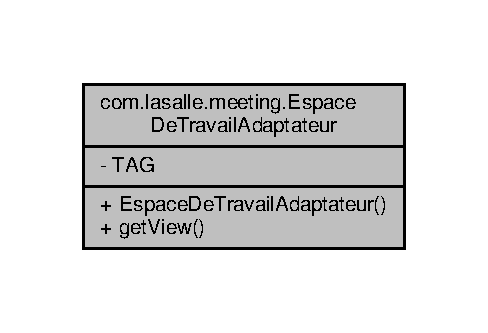
\includegraphics[width=234pt]{classcom_1_1lasalle_1_1meeting_1_1_espace_de_travail_adaptateur__coll__graph}
\end{center}
\end{figure}
\subsubsection*{Classes}
\begin{DoxyCompactItemize}
\item 
class \hyperlink{classcom_1_1lasalle_1_1meeting_1_1_espace_de_travail_adaptateur_1_1_view_holder}{View\+Holder}
\end{DoxyCompactItemize}
\subsubsection*{Fonctions membres publiques}
\begin{DoxyCompactItemize}
\item 
\hyperlink{classcom_1_1lasalle_1_1meeting_1_1_espace_de_travail_adaptateur_a236d4cbea7b551e4faf638b578c1f980}{Espace\+De\+Travail\+Adaptateur} (Context context, int resource, Vector$<$ \hyperlink{classcom_1_1lasalle_1_1meeting_1_1_espace_de_travail}{Espace\+De\+Travail} $>$ espaces\+De\+Travail)
\item 
View \hyperlink{classcom_1_1lasalle_1_1meeting_1_1_espace_de_travail_adaptateur_a288239cdb1a4e23274361c4a5dc503ba}{get\+View} (int position, View view, View\+Group parent)
\end{DoxyCompactItemize}
\subsubsection*{Attributs privés statiques}
\begin{DoxyCompactItemize}
\item 
static final String \hyperlink{classcom_1_1lasalle_1_1meeting_1_1_espace_de_travail_adaptateur_a6d9fb5167546f9b1da395ca3ce3a577f}{T\+AG} = \char`\"{}\+\_\+\+Espace\+De\+Travail\+Adaptateur\char`\"{}
\end{DoxyCompactItemize}


\subsubsection{Description détaillée}


Définition à la ligne \hyperlink{_espace_de_travail_adaptateur_8java_source_l00022}{22} du fichier \hyperlink{_espace_de_travail_adaptateur_8java_source}{Espace\+De\+Travail\+Adaptateur.\+java}.



\subsubsection{Documentation des constructeurs et destructeur}
\mbox{\Hypertarget{classcom_1_1lasalle_1_1meeting_1_1_espace_de_travail_adaptateur_a236d4cbea7b551e4faf638b578c1f980}\label{classcom_1_1lasalle_1_1meeting_1_1_espace_de_travail_adaptateur_a236d4cbea7b551e4faf638b578c1f980}} 
\index{com\+::lasalle\+::meeting\+::\+Espace\+De\+Travail\+Adaptateur@{com\+::lasalle\+::meeting\+::\+Espace\+De\+Travail\+Adaptateur}!Espace\+De\+Travail\+Adaptateur@{Espace\+De\+Travail\+Adaptateur}}
\index{Espace\+De\+Travail\+Adaptateur@{Espace\+De\+Travail\+Adaptateur}!com\+::lasalle\+::meeting\+::\+Espace\+De\+Travail\+Adaptateur@{com\+::lasalle\+::meeting\+::\+Espace\+De\+Travail\+Adaptateur}}
\paragraph{\texorpdfstring{Espace\+De\+Travail\+Adaptateur()}{EspaceDeTravailAdaptateur()}}
{\footnotesize\ttfamily com.\+lasalle.\+meeting.\+Espace\+De\+Travail\+Adaptateur.\+Espace\+De\+Travail\+Adaptateur (\begin{DoxyParamCaption}\item[{Context}]{context,  }\item[{int}]{resource,  }\item[{Vector$<$ \hyperlink{classcom_1_1lasalle_1_1meeting_1_1_espace_de_travail}{Espace\+De\+Travail} $>$}]{espaces\+De\+Travail }\end{DoxyParamCaption})}



Définition à la ligne \hyperlink{_espace_de_travail_adaptateur_8java_source_l00026}{26} du fichier \hyperlink{_espace_de_travail_adaptateur_8java_source}{Espace\+De\+Travail\+Adaptateur.\+java}.


\begin{DoxyCode}
00027     \{
00028         super(context, resource, espacesDeTravail);
00029         Log.d(\hyperlink{classcom_1_1lasalle_1_1meeting_1_1_espace_de_travail_adaptateur_a6d9fb5167546f9b1da395ca3ce3a577f}{TAG}, \textcolor{stringliteral}{"EspaceDeTravailAdaptateur()"});
00030     \}
\end{DoxyCode}


\subsubsection{Documentation des fonctions membres}
\mbox{\Hypertarget{classcom_1_1lasalle_1_1meeting_1_1_espace_de_travail_adaptateur_a288239cdb1a4e23274361c4a5dc503ba}\label{classcom_1_1lasalle_1_1meeting_1_1_espace_de_travail_adaptateur_a288239cdb1a4e23274361c4a5dc503ba}} 
\index{com\+::lasalle\+::meeting\+::\+Espace\+De\+Travail\+Adaptateur@{com\+::lasalle\+::meeting\+::\+Espace\+De\+Travail\+Adaptateur}!get\+View@{get\+View}}
\index{get\+View@{get\+View}!com\+::lasalle\+::meeting\+::\+Espace\+De\+Travail\+Adaptateur@{com\+::lasalle\+::meeting\+::\+Espace\+De\+Travail\+Adaptateur}}
\paragraph{\texorpdfstring{get\+View()}{getView()}}
{\footnotesize\ttfamily View com.\+lasalle.\+meeting.\+Espace\+De\+Travail\+Adaptateur.\+get\+View (\begin{DoxyParamCaption}\item[{int}]{position,  }\item[{View}]{view,  }\item[{View\+Group}]{parent }\end{DoxyParamCaption})}



Définition à la ligne \hyperlink{_espace_de_travail_adaptateur_8java_source_l00040}{40} du fichier \hyperlink{_espace_de_travail_adaptateur_8java_source}{Espace\+De\+Travail\+Adaptateur.\+java}.



Références \hyperlink{_espace_de_travail_8java_source_l00097}{com.\+lasalle.\+meeting.\+Espace\+De\+Travail.\+get\+Description()}, \hyperlink{_espace_de_travail_8java_source_l00117}{com.\+lasalle.\+meeting.\+Espace\+De\+Travail.\+get\+Est\+Reserve()}, et \hyperlink{_espace_de_travail_8java_source_l00087}{com.\+lasalle.\+meeting.\+Espace\+De\+Travail.\+get\+Nom()}.


\begin{DoxyCode}
00041     \{
00042         EspaceDeTravail espaceDeTravail = null;
00043         ViewHolder viewHolder;
00044 
00045         \textcolor{keywordflow}{if} (view == null)
00046         \{
00047             viewHolder = \textcolor{keyword}{new} ViewHolder();
00048             LayoutInflater inflater = LayoutInflater.from(getContext());
00049             view = inflater.inflate(R.layout.element\_espace\_travail, parent, \textcolor{keyword}{false});
00050             viewHolder.nomEspaceDeTravail = (TextView)view.findViewById(R.id.nomEspaceDeTravail);
00051             viewHolder.descriptionEspaceDeTravail = (TextView)view.findViewById(R.id.
      descriptionEspaceDeTravail);
00052             viewHolder.disponibiliteEspaceDeTravail = (TextView)view.findViewById(R.id.
      disponibiliteEspaceDeTravail);
00053             view.setTag(viewHolder);
00054         \}
00055         \textcolor{keywordflow}{else}
00056         \{
00057             viewHolder = (ViewHolder)view.getTag();
00058         \}
00059 
00060         espaceDeTravail = getItem(position);
00061         \textcolor{keywordflow}{if} (espaceDeTravail != null)
00062         \{
00063             \textcolor{comment}{//Log.d(TAG, "Nom : " + espaceDeTravail.getNom());}
00064             viewHolder.nomEspaceDeTravail.setText(espaceDeTravail.getNom());
00065             viewHolder.descriptionEspaceDeTravail.setText(espaceDeTravail.getDescription());
00066             \textcolor{keywordflow}{if}(!espaceDeTravail.getEstReserve())
00067             \{
00068                 viewHolder.disponibiliteEspaceDeTravail.setText(\textcolor{stringliteral}{"Libre"});
00069                 viewHolder.disponibiliteEspaceDeTravail.setTextColor(Color.parseColor(\textcolor{stringliteral}{"#00FF00"})); \textcolor{comment}{//
       Color.rgb(0,255,0)}
00070             \}
00071             \textcolor{keywordflow}{else}
00072             \{
00073                 viewHolder.disponibiliteEspaceDeTravail.setText(\textcolor{stringliteral}{"Occupé"});
00074                 viewHolder.disponibiliteEspaceDeTravail.setTextColor(Color.rgb(255,0,0));
00075             \}
00076         \}
00077 
00078         \textcolor{keywordflow}{return} view;
00079     \}
\end{DoxyCode}


\subsubsection{Documentation des données membres}
\mbox{\Hypertarget{classcom_1_1lasalle_1_1meeting_1_1_espace_de_travail_adaptateur_a6d9fb5167546f9b1da395ca3ce3a577f}\label{classcom_1_1lasalle_1_1meeting_1_1_espace_de_travail_adaptateur_a6d9fb5167546f9b1da395ca3ce3a577f}} 
\index{com\+::lasalle\+::meeting\+::\+Espace\+De\+Travail\+Adaptateur@{com\+::lasalle\+::meeting\+::\+Espace\+De\+Travail\+Adaptateur}!T\+AG@{T\+AG}}
\index{T\+AG@{T\+AG}!com\+::lasalle\+::meeting\+::\+Espace\+De\+Travail\+Adaptateur@{com\+::lasalle\+::meeting\+::\+Espace\+De\+Travail\+Adaptateur}}
\paragraph{\texorpdfstring{T\+AG}{TAG}}
{\footnotesize\ttfamily final String com.\+lasalle.\+meeting.\+Espace\+De\+Travail\+Adaptateur.\+T\+AG = \char`\"{}\+\_\+\+Espace\+De\+Travail\+Adaptateur\char`\"{}\hspace{0.3cm}{\ttfamily [static]}, {\ttfamily [private]}}



Définition à la ligne \hyperlink{_espace_de_travail_adaptateur_8java_source_l00024}{24} du fichier \hyperlink{_espace_de_travail_adaptateur_8java_source}{Espace\+De\+Travail\+Adaptateur.\+java}.



La documentation de cette classe a été générée à partir du fichier suivant \+:\begin{DoxyCompactItemize}
\item 
\hyperlink{_espace_de_travail_adaptateur_8java}{Espace\+De\+Travail\+Adaptateur.\+java}\end{DoxyCompactItemize}

\hypertarget{classcom_1_1lasalle_1_1meeting_1_1_i_h_m_meeting}{}\subsection{Référence de la classe com.\+lasalle.\+meeting.\+I\+H\+M\+Meeting}
\label{classcom_1_1lasalle_1_1meeting_1_1_i_h_m_meeting}\index{com.\+lasalle.\+meeting.\+I\+H\+M\+Meeting@{com.\+lasalle.\+meeting.\+I\+H\+M\+Meeting}}


L\textquotesingle{}activité principale de l\textquotesingle{}application Meeting.  




Graphe de collaboration de com.\+lasalle.\+meeting.\+I\+H\+M\+Meeting\+:\nopagebreak
\begin{figure}[H]
\begin{center}
\leavevmode
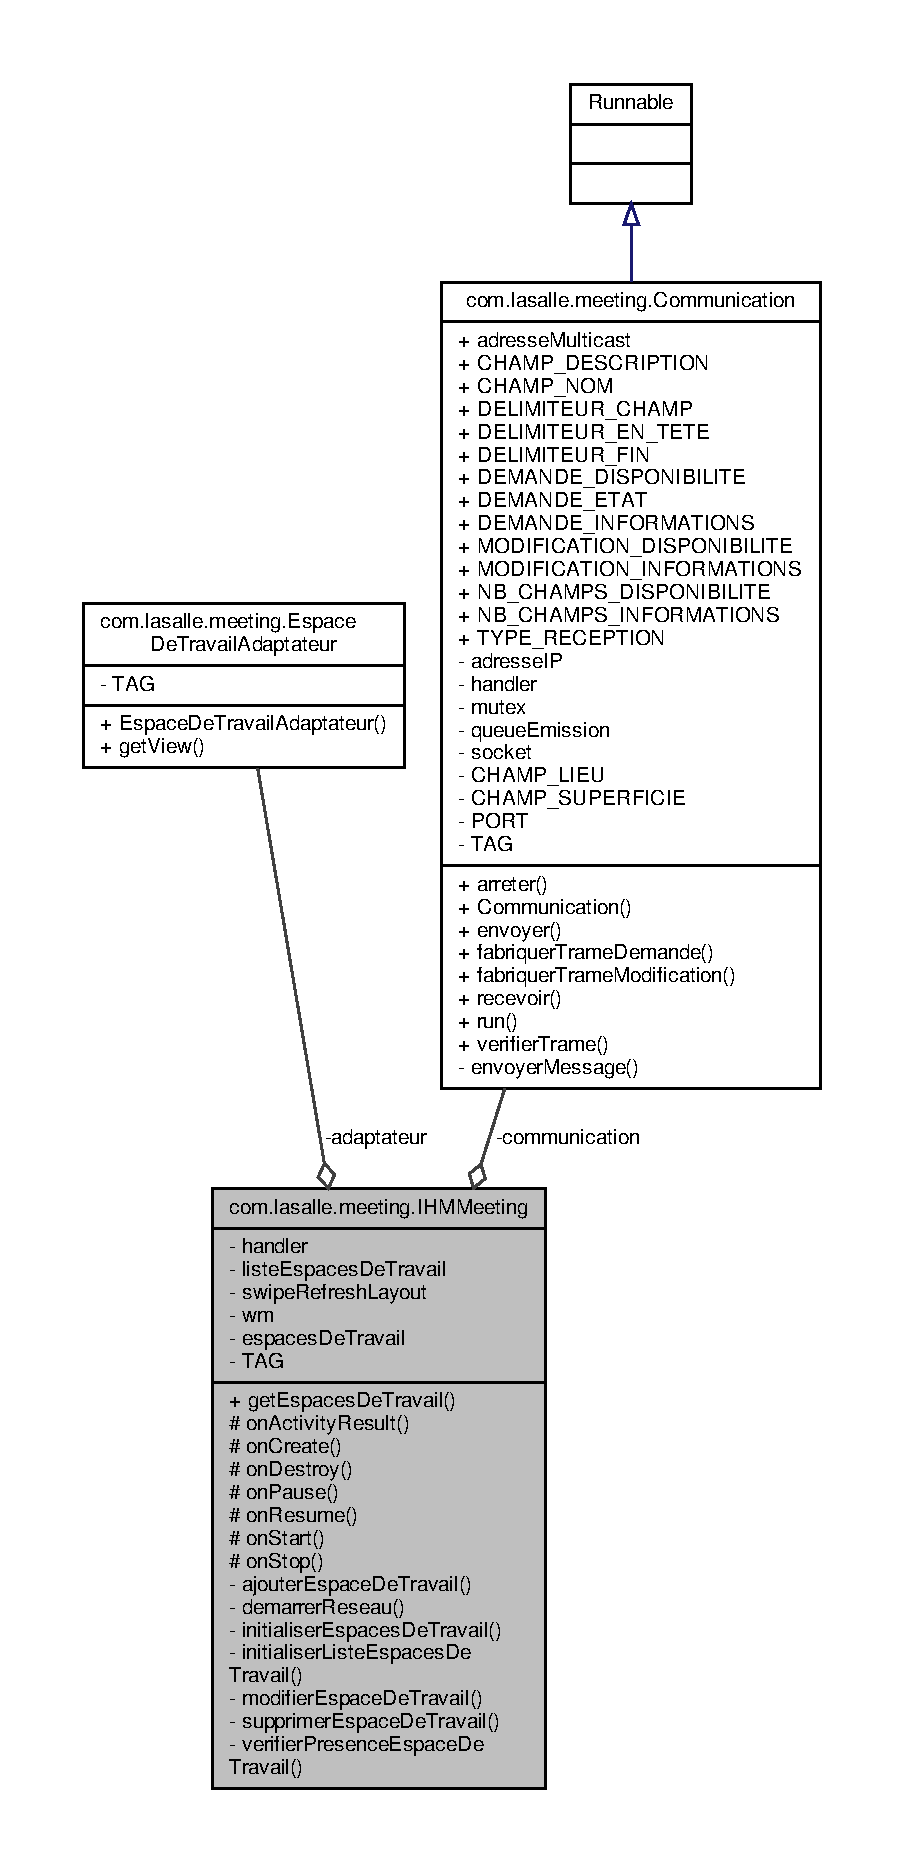
\includegraphics[height=550pt]{classcom_1_1lasalle_1_1meeting_1_1_i_h_m_meeting__coll__graph}
\end{center}
\end{figure}
\subsubsection*{Fonctions membres publiques statiques}
\begin{DoxyCompactItemize}
\item 
static Vector$<$ \hyperlink{classcom_1_1lasalle_1_1meeting_1_1_espace_de_travail}{Espace\+De\+Travail} $>$ \hyperlink{classcom_1_1lasalle_1_1meeting_1_1_i_h_m_meeting_aad942bca6cb6117dc57fb58142f0728c}{get\+Espaces\+De\+Travail} ()
\end{DoxyCompactItemize}
\subsubsection*{Fonctions membres protégées}
\begin{DoxyCompactItemize}
\item 
void \hyperlink{classcom_1_1lasalle_1_1meeting_1_1_i_h_m_meeting_aa7f5623eef9a049cf786ff15a4c63274}{on\+Activity\+Result} (int request\+Code, int result\+Code, Intent data)
\begin{DoxyCompactList}\small\item\em Traite le retour de l\textquotesingle{}activité d\textquotesingle{}affichage d\textquotesingle{}un espace de travail. \end{DoxyCompactList}\item 
void \hyperlink{classcom_1_1lasalle_1_1meeting_1_1_i_h_m_meeting_a34012ee88c1e079fef93ed115978d669}{on\+Create} (Bundle saved\+Instance\+State)
\begin{DoxyCompactList}\small\item\em Méthode appelée à la création de l\textquotesingle{}activité \end{DoxyCompactList}\item 
void \hyperlink{classcom_1_1lasalle_1_1meeting_1_1_i_h_m_meeting_a949a2219b9b5c29f7c1a9855a782a676}{on\+Destroy} ()
\begin{DoxyCompactList}\small\item\em Méthode appelée à la destruction de l\textquotesingle{}application (après \hyperlink{classcom_1_1lasalle_1_1meeting_1_1_i_h_m_meeting_a74e6b3e48ce9a26612916194d4692e6a}{on\+Stop()} et détruite par le système Android) \end{DoxyCompactList}\item 
void \hyperlink{classcom_1_1lasalle_1_1meeting_1_1_i_h_m_meeting_a1663a4b9bcff059ab95a72ca019cffb1}{on\+Pause} ()
\begin{DoxyCompactList}\small\item\em Méthode appelée après qu\textquotesingle{}une boîte de dialogue s\textquotesingle{}est affichée (on reprend sur un \hyperlink{classcom_1_1lasalle_1_1meeting_1_1_i_h_m_meeting_af9a99a4aa01c58f7d85e0d6e6d13eaa4}{on\+Resume()}) ou avant \hyperlink{classcom_1_1lasalle_1_1meeting_1_1_i_h_m_meeting_a74e6b3e48ce9a26612916194d4692e6a}{on\+Stop()} (activité plus visible) \end{DoxyCompactList}\item 
void \hyperlink{classcom_1_1lasalle_1_1meeting_1_1_i_h_m_meeting_af9a99a4aa01c58f7d85e0d6e6d13eaa4}{on\+Resume} ()
\begin{DoxyCompactList}\small\item\em Méthode appelée après \hyperlink{classcom_1_1lasalle_1_1meeting_1_1_i_h_m_meeting_a55bd9ed1bd85ada8c53930fb1650a954}{on\+Start()} ou après \hyperlink{classcom_1_1lasalle_1_1meeting_1_1_i_h_m_meeting_a1663a4b9bcff059ab95a72ca019cffb1}{on\+Pause()} \end{DoxyCompactList}\item 
void \hyperlink{classcom_1_1lasalle_1_1meeting_1_1_i_h_m_meeting_a55bd9ed1bd85ada8c53930fb1650a954}{on\+Start} ()
\begin{DoxyCompactList}\small\item\em Méthode appelée au démarrage de l\textquotesingle{}activité Main\+Activity. \end{DoxyCompactList}\item 
void \hyperlink{classcom_1_1lasalle_1_1meeting_1_1_i_h_m_meeting_a74e6b3e48ce9a26612916194d4692e6a}{on\+Stop} ()
\begin{DoxyCompactList}\small\item\em Méthode appelée lorsque l\textquotesingle{}activité n\textquotesingle{}est plus visible. \end{DoxyCompactList}\end{DoxyCompactItemize}
\subsubsection*{Fonctions membres privées}
\begin{DoxyCompactItemize}
\item 
void \hyperlink{classcom_1_1lasalle_1_1meeting_1_1_i_h_m_meeting_ad9ff630d7dc8df0155e3a552bfdfed75}{ajouter\+Espace\+De\+Travail} (\hyperlink{classcom_1_1lasalle_1_1meeting_1_1_espace_de_travail}{Espace\+De\+Travail} espace\+De\+Travail)
\begin{DoxyCompactList}\small\item\em Ajoute un espace de travail si pas encore détecté \end{DoxyCompactList}\item 
void \hyperlink{classcom_1_1lasalle_1_1meeting_1_1_i_h_m_meeting_ab9ef4bd3436aa480f92a5b1922fd6666}{demarrer\+Reseau} ()
\item 
void \hyperlink{classcom_1_1lasalle_1_1meeting_1_1_i_h_m_meeting_ad4660f416b16b6df0f96d58f4c36b6f6}{initialiser\+Espaces\+De\+Travail} ()
\begin{DoxyCompactList}\small\item\em Crée les espaces de travail détectés. \end{DoxyCompactList}\item 
void \hyperlink{classcom_1_1lasalle_1_1meeting_1_1_i_h_m_meeting_a6624feade3dc156bc7eb40f79cb47267}{initialiser\+Liste\+Espaces\+De\+Travail} ()
\begin{DoxyCompactList}\small\item\em Initialise la vue pour les espaces de travail. \end{DoxyCompactList}\item 
void \hyperlink{classcom_1_1lasalle_1_1meeting_1_1_i_h_m_meeting_a3367c0a9b9743ca7808cb2265789f9b8}{modifier\+Espace\+De\+Travail} (\hyperlink{classcom_1_1lasalle_1_1meeting_1_1_espace_de_travail}{Espace\+De\+Travail} espace\+De\+Travail)
\begin{DoxyCompactList}\small\item\em Modifie un espace de travail si déjà détecté \end{DoxyCompactList}\item 
void \hyperlink{classcom_1_1lasalle_1_1meeting_1_1_i_h_m_meeting_a1418ee16ded8b09f4c4a9c1a9359163a}{supprimer\+Espace\+De\+Travail} (\hyperlink{classcom_1_1lasalle_1_1meeting_1_1_espace_de_travail}{Espace\+De\+Travail} espace\+De\+Travail)
\begin{DoxyCompactList}\small\item\em Supprime un espace de travail si déjà détecté \end{DoxyCompactList}\item 
int \hyperlink{classcom_1_1lasalle_1_1meeting_1_1_i_h_m_meeting_a402dc23f375fae1f1faa3d5728cdad00}{verifier\+Presence\+Espace\+De\+Travail} (\hyperlink{classcom_1_1lasalle_1_1meeting_1_1_espace_de_travail}{Espace\+De\+Travail} espace\+De\+Travail)
\begin{DoxyCompactList}\small\item\em Vérifie la présence d\textquotesingle{}un espace de travail dans le conteneur des espaces de travail détectés. \end{DoxyCompactList}\end{DoxyCompactItemize}
\subsubsection*{Attributs privés}
\begin{DoxyCompactItemize}
\item 
\hyperlink{classcom_1_1lasalle_1_1meeting_1_1_espace_de_travail_adaptateur}{Espace\+De\+Travail\+Adaptateur} \hyperlink{classcom_1_1lasalle_1_1meeting_1_1_i_h_m_meeting_ac103010077163ba43b830ffe524f476d}{adaptateur}
\begin{DoxyCompactList}\small\item\em Adaptateur pour les espaces de travail. \end{DoxyCompactList}\item 
Handler \hyperlink{classcom_1_1lasalle_1_1meeting_1_1_i_h_m_meeting_af0a341dd3f520bba9d94b4b083ff75af}{handler}
\begin{DoxyCompactList}\small\item\em permet de récuperer les trames \end{DoxyCompactList}\item 
List\+View \hyperlink{classcom_1_1lasalle_1_1meeting_1_1_i_h_m_meeting_ae32ea3420cbe17af0b32df447e326427}{liste\+Espaces\+De\+Travail}
\begin{DoxyCompactList}\small\item\em Affichage des espaces de travail sous forme de liste. \end{DoxyCompactList}\item 
Swipe\+Refresh\+Layout \hyperlink{classcom_1_1lasalle_1_1meeting_1_1_i_h_m_meeting_a64f84fda5f7f595cf0c75ccfb189af8d}{swipe\+Refresh\+Layout}
\begin{DoxyCompactList}\small\item\em pour le Pull To Refresh \end{DoxyCompactList}\item 
Wifi\+Manager \hyperlink{classcom_1_1lasalle_1_1meeting_1_1_i_h_m_meeting_acdbac7f6ea8e7a8ed99e0ceaaf0f9f97}{wm} = null
\begin{DoxyCompactList}\small\item\em attribut permettant de voir la connection au Wi\+Fi \end{DoxyCompactList}\end{DoxyCompactItemize}
\subsubsection*{Attributs privés statiques}
\begin{DoxyCompactItemize}
\item 
static \hyperlink{classcom_1_1lasalle_1_1meeting_1_1_communication}{Communication} \hyperlink{classcom_1_1lasalle_1_1meeting_1_1_i_h_m_meeting_a12567e2164a68e0cbe74487935c1263e}{communication} = null
\begin{DoxyCompactList}\small\item\em attribut permettant d\textquotesingle{}envoyer des requêtes \end{DoxyCompactList}\item 
static Vector$<$ \hyperlink{classcom_1_1lasalle_1_1meeting_1_1_espace_de_travail}{Espace\+De\+Travail} $>$ \hyperlink{classcom_1_1lasalle_1_1meeting_1_1_i_h_m_meeting_acba41978aec60c27f07db774f9b68b68}{espaces\+De\+Travail}
\begin{DoxyCompactList}\small\item\em Conteneur pour les espaces de travail. \end{DoxyCompactList}\item 
static final String \hyperlink{classcom_1_1lasalle_1_1meeting_1_1_i_h_m_meeting_a239eafcb0ccc896bdba538d1c0f08e65}{T\+AG} = \char`\"{}\+\_\+\+I\+H\+M\+Meeting\char`\"{}
\begin{DoxyCompactList}\small\item\em T\+AG pour les logs. \end{DoxyCompactList}\end{DoxyCompactItemize}


\subsubsection{Description détaillée}
L\textquotesingle{}activité principale de l\textquotesingle{}application Meeting. 

Définition à la ligne \hyperlink{_i_h_m_meeting_8java_source_l00035}{35} du fichier \hyperlink{_i_h_m_meeting_8java_source}{I\+H\+M\+Meeting.\+java}.



\subsubsection{Documentation des fonctions membres}
\mbox{\Hypertarget{classcom_1_1lasalle_1_1meeting_1_1_i_h_m_meeting_ad9ff630d7dc8df0155e3a552bfdfed75}\label{classcom_1_1lasalle_1_1meeting_1_1_i_h_m_meeting_ad9ff630d7dc8df0155e3a552bfdfed75}} 
\index{com\+::lasalle\+::meeting\+::\+I\+H\+M\+Meeting@{com\+::lasalle\+::meeting\+::\+I\+H\+M\+Meeting}!ajouter\+Espace\+De\+Travail@{ajouter\+Espace\+De\+Travail}}
\index{ajouter\+Espace\+De\+Travail@{ajouter\+Espace\+De\+Travail}!com\+::lasalle\+::meeting\+::\+I\+H\+M\+Meeting@{com\+::lasalle\+::meeting\+::\+I\+H\+M\+Meeting}}
\paragraph{\texorpdfstring{ajouter\+Espace\+De\+Travail()}{ajouterEspaceDeTravail()}}
{\footnotesize\ttfamily void com.\+lasalle.\+meeting.\+I\+H\+M\+Meeting.\+ajouter\+Espace\+De\+Travail (\begin{DoxyParamCaption}\item[{\hyperlink{classcom_1_1lasalle_1_1meeting_1_1_espace_de_travail}{Espace\+De\+Travail}}]{espace\+De\+Travail }\end{DoxyParamCaption})\hspace{0.3cm}{\ttfamily [private]}}



Ajoute un espace de travail si pas encore détecté 


\begin{DoxyParams}{Paramètres}
{\em espace\+De\+Travail} & un espace de travail \\
\hline
\end{DoxyParams}


Définition à la ligne \hyperlink{_i_h_m_meeting_8java_source_l00199}{199} du fichier \hyperlink{_i_h_m_meeting_8java_source}{I\+H\+M\+Meeting.\+java}.



Références \hyperlink{_i_h_m_meeting_8java_source_l00248}{com.\+lasalle.\+meeting.\+I\+H\+M\+Meeting.\+verifier\+Presence\+Espace\+De\+Travail()}.



Référencé par \hyperlink{_i_h_m_meeting_8java_source_l00171}{com.\+lasalle.\+meeting.\+I\+H\+M\+Meeting.\+initialiser\+Espaces\+De\+Travail()}.


\begin{DoxyCode}
00200     \{
00201         \textcolor{keywordtype}{int} position = \hyperlink{classcom_1_1lasalle_1_1meeting_1_1_i_h_m_meeting_a402dc23f375fae1f1faa3d5728cdad00}{verifierPresenceEspaceDeTravail}(espaceDeTravail);
00202 
00203         \textcolor{keywordflow}{if}(position == -1)
00204         \{
00205             \hyperlink{classcom_1_1lasalle_1_1meeting_1_1_i_h_m_meeting_acba41978aec60c27f07db774f9b68b68}{espacesDeTravail}.add(espaceDeTravail);
00206             \hyperlink{classcom_1_1lasalle_1_1meeting_1_1_i_h_m_meeting_ac103010077163ba43b830ffe524f476d}{adaptateur}.notifyDataSetChanged();
00207         \}
00208     \}
\end{DoxyCode}
\mbox{\Hypertarget{classcom_1_1lasalle_1_1meeting_1_1_i_h_m_meeting_ab9ef4bd3436aa480f92a5b1922fd6666}\label{classcom_1_1lasalle_1_1meeting_1_1_i_h_m_meeting_ab9ef4bd3436aa480f92a5b1922fd6666}} 
\index{com\+::lasalle\+::meeting\+::\+I\+H\+M\+Meeting@{com\+::lasalle\+::meeting\+::\+I\+H\+M\+Meeting}!demarrer\+Reseau@{demarrer\+Reseau}}
\index{demarrer\+Reseau@{demarrer\+Reseau}!com\+::lasalle\+::meeting\+::\+I\+H\+M\+Meeting@{com\+::lasalle\+::meeting\+::\+I\+H\+M\+Meeting}}
\paragraph{\texorpdfstring{demarrer\+Reseau()}{demarrerReseau()}}
{\footnotesize\ttfamily void com.\+lasalle.\+meeting.\+I\+H\+M\+Meeting.\+demarrer\+Reseau (\begin{DoxyParamCaption}{ }\end{DoxyParamCaption})\hspace{0.3cm}{\ttfamily [private]}}



Définition à la ligne \hyperlink{_i_h_m_meeting_8java_source_l00082}{82} du fichier \hyperlink{_i_h_m_meeting_8java_source}{I\+H\+M\+Meeting.\+java}.



Références \hyperlink{_communication_8java_source_l00040}{com.\+lasalle.\+meeting.\+Communication.\+adresse\+Multicast}, \hyperlink{_communication_8java_source_l00055}{com.\+lasalle.\+meeting.\+Communication.\+D\+E\+M\+A\+N\+D\+E\+\_\+\+E\+T\+AT}, \hyperlink{_communication_8java_source_l00090}{com.\+lasalle.\+meeting.\+Communication.\+envoyer()}, \hyperlink{_communication_8java_source_l00180}{com.\+lasalle.\+meeting.\+Communication.\+fabriquer\+Trame\+Demande()}, et \hyperlink{_i_h_m_meeting_8java_source_l00311}{com.\+lasalle.\+meeting.\+I\+H\+M\+Meeting.\+handler}.



Référencé par \hyperlink{_i_h_m_meeting_8java_source_l00060}{com.\+lasalle.\+meeting.\+I\+H\+M\+Meeting.\+on\+Create()}.


\begin{DoxyCode}
00083     \{
00084         \hyperlink{classcom_1_1lasalle_1_1meeting_1_1_i_h_m_meeting_acdbac7f6ea8e7a8ed99e0ceaaf0f9f97}{wm} = (WifiManager) getApplicationContext().getSystemService(Context.WIFI\_SERVICE);
00085         \textcolor{keywordflow}{if} (!\hyperlink{classcom_1_1lasalle_1_1meeting_1_1_i_h_m_meeting_acdbac7f6ea8e7a8ed99e0ceaaf0f9f97}{wm}.isWifiEnabled())
00086         \{
00087             Log.d(\hyperlink{classcom_1_1lasalle_1_1meeting_1_1_i_h_m_meeting_a239eafcb0ccc896bdba538d1c0f08e65}{TAG}, \textcolor{stringliteral}{"WiFi indisponible !"});
00088             \hyperlink{classcom_1_1lasalle_1_1meeting_1_1_i_h_m_meeting_acdbac7f6ea8e7a8ed99e0ceaaf0f9f97}{wm}.setWifiEnabled(\textcolor{keyword}{true});
00089         \}
00090         \textcolor{keywordflow}{else}
00091         \{
00092             Log.d(\hyperlink{classcom_1_1lasalle_1_1meeting_1_1_i_h_m_meeting_a239eafcb0ccc896bdba538d1c0f08e65}{TAG}, \textcolor{stringliteral}{"WiFi disponible"});
00093         \}
00094 
00095         \hyperlink{classcom_1_1lasalle_1_1meeting_1_1_i_h_m_meeting_a12567e2164a68e0cbe74487935c1263e}{communication} = \textcolor{keyword}{new} Communication(\hyperlink{classcom_1_1lasalle_1_1meeting_1_1_i_h_m_meeting_af0a341dd3f520bba9d94b4b083ff75af}{handler});
00096 
00097         \textcolor{comment}{// Démarre la réception des trames des portiers}
00098         Thread tCommunicationUDP = \textcolor{keyword}{new} Thread(\hyperlink{classcom_1_1lasalle_1_1meeting_1_1_i_h_m_meeting_a12567e2164a68e0cbe74487935c1263e}{communication}, \textcolor{stringliteral}{"Communication"});
00099         tCommunicationUDP.start(); \textcolor{comment}{// execute la méthode run()}
00100 
00101         \textcolor{comment}{// Test}
00102         \textcolor{keywordflow}{if}(\hyperlink{classcom_1_1lasalle_1_1meeting_1_1_i_h_m_meeting_a12567e2164a68e0cbe74487935c1263e}{communication} != null)
00103         \{
00104             \textcolor{comment}{// demande l'état des portiers joignables}
00105             \hyperlink{classcom_1_1lasalle_1_1meeting_1_1_i_h_m_meeting_a12567e2164a68e0cbe74487935c1263e}{communication}.\hyperlink{classcom_1_1lasalle_1_1meeting_1_1_communication_a03f0e419513d7f33900dde412e2a4471}{envoyer}(\hyperlink{classcom_1_1lasalle_1_1meeting_1_1_i_h_m_meeting_a12567e2164a68e0cbe74487935c1263e}{communication}.
      \hyperlink{classcom_1_1lasalle_1_1meeting_1_1_communication_a3b07023cb3f3a1549da711b5c6ba6af1}{fabriquerTrameDemande}(Communication.DEMANDE\_ETAT), Communication.adresseMulticast); \textcolor{comment}{//
       voir protocole}
00106         \}
00107     \}
\end{DoxyCode}
\mbox{\Hypertarget{classcom_1_1lasalle_1_1meeting_1_1_i_h_m_meeting_aad942bca6cb6117dc57fb58142f0728c}\label{classcom_1_1lasalle_1_1meeting_1_1_i_h_m_meeting_aad942bca6cb6117dc57fb58142f0728c}} 
\index{com\+::lasalle\+::meeting\+::\+I\+H\+M\+Meeting@{com\+::lasalle\+::meeting\+::\+I\+H\+M\+Meeting}!get\+Espaces\+De\+Travail@{get\+Espaces\+De\+Travail}}
\index{get\+Espaces\+De\+Travail@{get\+Espaces\+De\+Travail}!com\+::lasalle\+::meeting\+::\+I\+H\+M\+Meeting@{com\+::lasalle\+::meeting\+::\+I\+H\+M\+Meeting}}
\paragraph{\texorpdfstring{get\+Espaces\+De\+Travail()}{getEspacesDeTravail()}}
{\footnotesize\ttfamily static Vector$<$\hyperlink{classcom_1_1lasalle_1_1meeting_1_1_espace_de_travail}{Espace\+De\+Travail}$>$ com.\+lasalle.\+meeting.\+I\+H\+M\+Meeting.\+get\+Espaces\+De\+Travail (\begin{DoxyParamCaption}{ }\end{DoxyParamCaption})\hspace{0.3cm}{\ttfamily [static]}}



Définition à la ligne \hyperlink{_i_h_m_meeting_8java_source_l00163}{163} du fichier \hyperlink{_i_h_m_meeting_8java_source}{I\+H\+M\+Meeting.\+java}.



Références \hyperlink{_i_h_m_meeting_8java_source_l00051}{com.\+lasalle.\+meeting.\+I\+H\+M\+Meeting.\+espaces\+De\+Travail}.


\begin{DoxyCode}
00164     \{
00165         \textcolor{keywordflow}{return} \hyperlink{classcom_1_1lasalle_1_1meeting_1_1_i_h_m_meeting_acba41978aec60c27f07db774f9b68b68}{espacesDeTravail};
00166     \}
\end{DoxyCode}
\mbox{\Hypertarget{classcom_1_1lasalle_1_1meeting_1_1_i_h_m_meeting_ad4660f416b16b6df0f96d58f4c36b6f6}\label{classcom_1_1lasalle_1_1meeting_1_1_i_h_m_meeting_ad4660f416b16b6df0f96d58f4c36b6f6}} 
\index{com\+::lasalle\+::meeting\+::\+I\+H\+M\+Meeting@{com\+::lasalle\+::meeting\+::\+I\+H\+M\+Meeting}!initialiser\+Espaces\+De\+Travail@{initialiser\+Espaces\+De\+Travail}}
\index{initialiser\+Espaces\+De\+Travail@{initialiser\+Espaces\+De\+Travail}!com\+::lasalle\+::meeting\+::\+I\+H\+M\+Meeting@{com\+::lasalle\+::meeting\+::\+I\+H\+M\+Meeting}}
\paragraph{\texorpdfstring{initialiser\+Espaces\+De\+Travail()}{initialiserEspacesDeTravail()}}
{\footnotesize\ttfamily void com.\+lasalle.\+meeting.\+I\+H\+M\+Meeting.\+initialiser\+Espaces\+De\+Travail (\begin{DoxyParamCaption}{ }\end{DoxyParamCaption})\hspace{0.3cm}{\ttfamily [private]}}



Crée les espaces de travail détectés. 



Définition à la ligne \hyperlink{_i_h_m_meeting_8java_source_l00171}{171} du fichier \hyperlink{_i_h_m_meeting_8java_source}{I\+H\+M\+Meeting.\+java}.



Références \hyperlink{_i_h_m_meeting_8java_source_l00199}{com.\+lasalle.\+meeting.\+I\+H\+M\+Meeting.\+ajouter\+Espace\+De\+Travail()}.



Référencé par \hyperlink{_i_h_m_meeting_8java_source_l00263}{com.\+lasalle.\+meeting.\+I\+H\+M\+Meeting.\+initialiser\+Liste\+Espaces\+De\+Travail()}, \hyperlink{_i_h_m_meeting_8java_source_l00060}{com.\+lasalle.\+meeting.\+I\+H\+M\+Meeting.\+on\+Create()}, et \hyperlink{_i_h_m_meeting_8java_source_l00114}{com.\+lasalle.\+meeting.\+I\+H\+M\+Meeting.\+on\+Start()}.


\begin{DoxyCode}
00172     \{
00173         Log.d(\hyperlink{classcom_1_1lasalle_1_1meeting_1_1_i_h_m_meeting_a239eafcb0ccc896bdba538d1c0f08e65}{TAG}, \textcolor{stringliteral}{"initialiserEspacesDeTravail()"});
00174 
00175         \textcolor{comment}{// Pour les tests}
00176         List<EspaceDeTravail> tous = Arrays.asList(
00177                 \textcolor{keyword}{new} EspaceDeTravail(\textcolor{stringliteral}{""}, \textcolor{stringliteral}{"B11"}, \textcolor{stringliteral}{"Bâtiment BTS"}, \textcolor{stringliteral}{"Salle de cours SN"}, 25, 20, 1, \textcolor{keyword}{false}),
00178                 \textcolor{keyword}{new} EspaceDeTravail( \textcolor{stringliteral}{""}, \textcolor{stringliteral}{"B20"}, \textcolor{stringliteral}{"Bâtiment BTS"}, \textcolor{stringliteral}{"Atelier"}, 100, 24, 1, \textcolor{keyword}{false}),
00179                 \textcolor{keyword}{new} EspaceDeTravail( \textcolor{stringliteral}{""}, \textcolor{stringliteral}{"B21"}, \textcolor{stringliteral}{"Bâtiment BTS"}, \textcolor{stringliteral}{"Salle de physique"}, 60, 22, 1, \textcolor{keyword}{false}),
00180                 \textcolor{keyword}{new} EspaceDeTravail( \textcolor{stringliteral}{""}, \textcolor{stringliteral}{"B22"}, \textcolor{stringliteral}{"Bâtiment BTS"}, \textcolor{stringliteral}{"Salle de cours"}, 60, 22, 1, \textcolor{keyword}{false})
00181         );
00182         \textcolor{comment}{//final int nbEspacesDeTravail = tous.size();}
00183         \textcolor{keyword}{final} \textcolor{keywordtype}{int} nbEspacesDeTravail = \textcolor{keyword}{new} Random().nextInt(tous.size());
00184         Log.d(\hyperlink{classcom_1_1lasalle_1_1meeting_1_1_i_h_m_meeting_a239eafcb0ccc896bdba538d1c0f08e65}{TAG}, \textcolor{stringliteral}{"nbEspacesDeTravail = "} + nbEspacesDeTravail);
00185 
00186         \textcolor{comment}{//espacesDeTravail.clear();}
00187         \textcolor{keywordflow}{for}(\textcolor{keywordtype}{int} i =0; i < nbEspacesDeTravail; i++)
00188         \{
00189             \hyperlink{classcom_1_1lasalle_1_1meeting_1_1_i_h_m_meeting_ad9ff630d7dc8df0155e3a552bfdfed75}{ajouterEspaceDeTravail}(tous.get(i));
00190         \}
00191 
00192         \hyperlink{classcom_1_1lasalle_1_1meeting_1_1_i_h_m_meeting_a64f84fda5f7f595cf0c75ccfb189af8d}{swipeRefreshLayout}.setRefreshing(\textcolor{keyword}{false}); \textcolor{comment}{// arrête le Pull To Refresh}
00193     \}
\end{DoxyCode}
\mbox{\Hypertarget{classcom_1_1lasalle_1_1meeting_1_1_i_h_m_meeting_a6624feade3dc156bc7eb40f79cb47267}\label{classcom_1_1lasalle_1_1meeting_1_1_i_h_m_meeting_a6624feade3dc156bc7eb40f79cb47267}} 
\index{com\+::lasalle\+::meeting\+::\+I\+H\+M\+Meeting@{com\+::lasalle\+::meeting\+::\+I\+H\+M\+Meeting}!initialiser\+Liste\+Espaces\+De\+Travail@{initialiser\+Liste\+Espaces\+De\+Travail}}
\index{initialiser\+Liste\+Espaces\+De\+Travail@{initialiser\+Liste\+Espaces\+De\+Travail}!com\+::lasalle\+::meeting\+::\+I\+H\+M\+Meeting@{com\+::lasalle\+::meeting\+::\+I\+H\+M\+Meeting}}
\paragraph{\texorpdfstring{initialiser\+Liste\+Espaces\+De\+Travail()}{initialiserListeEspacesDeTravail()}}
{\footnotesize\ttfamily void com.\+lasalle.\+meeting.\+I\+H\+M\+Meeting.\+initialiser\+Liste\+Espaces\+De\+Travail (\begin{DoxyParamCaption}{ }\end{DoxyParamCaption})\hspace{0.3cm}{\ttfamily [private]}}



Initialise la vue pour les espaces de travail. 



Définition à la ligne \hyperlink{_i_h_m_meeting_8java_source_l00263}{263} du fichier \hyperlink{_i_h_m_meeting_8java_source}{I\+H\+M\+Meeting.\+java}.



Références \hyperlink{_i_h_m_meeting_8java_source_l00171}{com.\+lasalle.\+meeting.\+I\+H\+M\+Meeting.\+initialiser\+Espaces\+De\+Travail()}.



Référencé par \hyperlink{_i_h_m_meeting_8java_source_l00060}{com.\+lasalle.\+meeting.\+I\+H\+M\+Meeting.\+on\+Create()}.


\begin{DoxyCode}
00264     \{
00265         Log.d(\hyperlink{classcom_1_1lasalle_1_1meeting_1_1_i_h_m_meeting_a239eafcb0ccc896bdba538d1c0f08e65}{TAG}, \textcolor{stringliteral}{"initialiserListeEspacesDeTravail()"});
00266 
00267         \hyperlink{classcom_1_1lasalle_1_1meeting_1_1_i_h_m_meeting_acba41978aec60c27f07db774f9b68b68}{espacesDeTravail} = \textcolor{keyword}{new} Vector<EspaceDeTravail>();
00268 
00269         \hyperlink{classcom_1_1lasalle_1_1meeting_1_1_i_h_m_meeting_ae32ea3420cbe17af0b32df447e326427}{listeEspacesDeTravail} = (ListView)findViewById(R.id.listeEspacesDeTravail);
00270 
00271         \hyperlink{classcom_1_1lasalle_1_1meeting_1_1_i_h_m_meeting_ac103010077163ba43b830ffe524f476d}{adaptateur} = \textcolor{keyword}{new} EspaceDeTravailAdaptateur(\textcolor{keyword}{this}, R.layout.element\_espace\_travail, 
      \hyperlink{classcom_1_1lasalle_1_1meeting_1_1_i_h_m_meeting_acba41978aec60c27f07db774f9b68b68}{espacesDeTravail});
00272 
00273         \hyperlink{classcom_1_1lasalle_1_1meeting_1_1_i_h_m_meeting_ad4660f416b16b6df0f96d58f4c36b6f6}{initialiserEspacesDeTravail}();
00274 
00275         listeEspacesDeTravail.setAdapter(\hyperlink{classcom_1_1lasalle_1_1meeting_1_1_i_h_m_meeting_ac103010077163ba43b830ffe524f476d}{adaptateur});
00276         \hyperlink{classcom_1_1lasalle_1_1meeting_1_1_i_h_m_meeting_ac103010077163ba43b830ffe524f476d}{adaptateur}.setNotifyOnChange(\textcolor{keyword}{true});
00277 
00278         listeEspacesDeTravail.setOnItemClickListener(
00279             \textcolor{keyword}{new} AdapterView.OnItemClickListener()
00280             \{
00281                 @Override
00282                 \textcolor{keyword}{public} \textcolor{keywordtype}{void} onItemClick(AdapterView<?> a, View v, \textcolor{keywordtype}{int} position, \textcolor{keywordtype}{long} \textcolor{keywordtype}{id})
00283                 \{
00284                     Log.d(\hyperlink{classcom_1_1lasalle_1_1meeting_1_1_i_h_m_meeting_a239eafcb0ccc896bdba538d1c0f08e65}{TAG}, \textcolor{stringliteral}{"Position : "} + position + \textcolor{stringliteral}{" - "} + \textcolor{stringliteral}{" Nom : "} + 
      \hyperlink{classcom_1_1lasalle_1_1meeting_1_1_i_h_m_meeting_acba41978aec60c27f07db774f9b68b68}{espacesDeTravail}.get(position).getNom());
00285                     Intent intent = \textcolor{keyword}{new} Intent(IHMMeeting.this, AffichageEspaceDeTravail.class);
00286                     intent.putExtra(\textcolor{stringliteral}{"unEspaceDeTravail"}, (Serializable)
      \hyperlink{classcom_1_1lasalle_1_1meeting_1_1_i_h_m_meeting_acba41978aec60c27f07db774f9b68b68}{espacesDeTravail}.get(position));
00287                     startActivityForResult(intent, 0);
00288                 \}
00289             \}
00290         );
00291     \}
\end{DoxyCode}
\mbox{\Hypertarget{classcom_1_1lasalle_1_1meeting_1_1_i_h_m_meeting_a3367c0a9b9743ca7808cb2265789f9b8}\label{classcom_1_1lasalle_1_1meeting_1_1_i_h_m_meeting_a3367c0a9b9743ca7808cb2265789f9b8}} 
\index{com\+::lasalle\+::meeting\+::\+I\+H\+M\+Meeting@{com\+::lasalle\+::meeting\+::\+I\+H\+M\+Meeting}!modifier\+Espace\+De\+Travail@{modifier\+Espace\+De\+Travail}}
\index{modifier\+Espace\+De\+Travail@{modifier\+Espace\+De\+Travail}!com\+::lasalle\+::meeting\+::\+I\+H\+M\+Meeting@{com\+::lasalle\+::meeting\+::\+I\+H\+M\+Meeting}}
\paragraph{\texorpdfstring{modifier\+Espace\+De\+Travail()}{modifierEspaceDeTravail()}}
{\footnotesize\ttfamily void com.\+lasalle.\+meeting.\+I\+H\+M\+Meeting.\+modifier\+Espace\+De\+Travail (\begin{DoxyParamCaption}\item[{\hyperlink{classcom_1_1lasalle_1_1meeting_1_1_espace_de_travail}{Espace\+De\+Travail}}]{espace\+De\+Travail }\end{DoxyParamCaption})\hspace{0.3cm}{\ttfamily [private]}}



Modifie un espace de travail si déjà détecté 


\begin{DoxyParams}{Paramètres}
{\em espace\+De\+Travail} & l\textquotesingle{}espace de travail modifié \\
\hline
\end{DoxyParams}


Définition à la ligne \hyperlink{_i_h_m_meeting_8java_source_l00214}{214} du fichier \hyperlink{_i_h_m_meeting_8java_source}{I\+H\+M\+Meeting.\+java}.



Références \hyperlink{_i_h_m_meeting_8java_source_l00248}{com.\+lasalle.\+meeting.\+I\+H\+M\+Meeting.\+verifier\+Presence\+Espace\+De\+Travail()}.



Référencé par \hyperlink{_i_h_m_meeting_8java_source_l00297}{com.\+lasalle.\+meeting.\+I\+H\+M\+Meeting.\+on\+Activity\+Result()}.


\begin{DoxyCode}
00215     \{
00216         \textcolor{keywordtype}{int} position = \hyperlink{classcom_1_1lasalle_1_1meeting_1_1_i_h_m_meeting_a402dc23f375fae1f1faa3d5728cdad00}{verifierPresenceEspaceDeTravail}(espaceDeTravail);
00217         Log.d(\hyperlink{classcom_1_1lasalle_1_1meeting_1_1_i_h_m_meeting_a239eafcb0ccc896bdba538d1c0f08e65}{TAG}, \textcolor{stringliteral}{"modifierEspaceDeTravail() : position = "} + position);
00218 
00219         \textcolor{keywordflow}{if}(position != -1)
00220         \{
00221             \textcolor{comment}{//espacesDeTravail.removeElementAt(position);}
00222             \textcolor{comment}{//espacesDeTravail.add(espaceDeTravail);}
00223             \hyperlink{classcom_1_1lasalle_1_1meeting_1_1_i_h_m_meeting_acba41978aec60c27f07db774f9b68b68}{espacesDeTravail}.set(position, espaceDeTravail);
00224             \hyperlink{classcom_1_1lasalle_1_1meeting_1_1_i_h_m_meeting_ac103010077163ba43b830ffe524f476d}{adaptateur}.notifyDataSetChanged();
00225         \}
00226     \}
\end{DoxyCode}
\mbox{\Hypertarget{classcom_1_1lasalle_1_1meeting_1_1_i_h_m_meeting_aa7f5623eef9a049cf786ff15a4c63274}\label{classcom_1_1lasalle_1_1meeting_1_1_i_h_m_meeting_aa7f5623eef9a049cf786ff15a4c63274}} 
\index{com\+::lasalle\+::meeting\+::\+I\+H\+M\+Meeting@{com\+::lasalle\+::meeting\+::\+I\+H\+M\+Meeting}!on\+Activity\+Result@{on\+Activity\+Result}}
\index{on\+Activity\+Result@{on\+Activity\+Result}!com\+::lasalle\+::meeting\+::\+I\+H\+M\+Meeting@{com\+::lasalle\+::meeting\+::\+I\+H\+M\+Meeting}}
\paragraph{\texorpdfstring{on\+Activity\+Result()}{onActivityResult()}}
{\footnotesize\ttfamily void com.\+lasalle.\+meeting.\+I\+H\+M\+Meeting.\+on\+Activity\+Result (\begin{DoxyParamCaption}\item[{int}]{request\+Code,  }\item[{int}]{result\+Code,  }\item[{Intent}]{data }\end{DoxyParamCaption})\hspace{0.3cm}{\ttfamily [protected]}}



Traite le retour de l\textquotesingle{}activité d\textquotesingle{}affichage d\textquotesingle{}un espace de travail. 



Définition à la ligne \hyperlink{_i_h_m_meeting_8java_source_l00297}{297} du fichier \hyperlink{_i_h_m_meeting_8java_source}{I\+H\+M\+Meeting.\+java}.



Références \hyperlink{_espace_de_travail_8java_source_l00117}{com.\+lasalle.\+meeting.\+Espace\+De\+Travail.\+get\+Est\+Reserve()}, et \hyperlink{_i_h_m_meeting_8java_source_l00214}{com.\+lasalle.\+meeting.\+I\+H\+M\+Meeting.\+modifier\+Espace\+De\+Travail()}.


\begin{DoxyCode}
00298     \{
00299         super.onActivityResult(requestCode, resultCode, data);
00300         EspaceDeTravail espaceDeTravail = (EspaceDeTravail)data.getSerializableExtra(\textcolor{stringliteral}{"unEspaceDeTravail"});
00301         Log.d(\hyperlink{classcom_1_1lasalle_1_1meeting_1_1_i_h_m_meeting_a239eafcb0ccc896bdba538d1c0f08e65}{TAG}, \textcolor{stringliteral}{"onActivityResult() espaceDeTravail : "} + espaceDeTravail.getEstReserve());
00302 
00303         \hyperlink{classcom_1_1lasalle_1_1meeting_1_1_i_h_m_meeting_a3367c0a9b9743ca7808cb2265789f9b8}{modifierEspaceDeTravail}(espaceDeTravail);
00304     \}
\end{DoxyCode}
\mbox{\Hypertarget{classcom_1_1lasalle_1_1meeting_1_1_i_h_m_meeting_a34012ee88c1e079fef93ed115978d669}\label{classcom_1_1lasalle_1_1meeting_1_1_i_h_m_meeting_a34012ee88c1e079fef93ed115978d669}} 
\index{com\+::lasalle\+::meeting\+::\+I\+H\+M\+Meeting@{com\+::lasalle\+::meeting\+::\+I\+H\+M\+Meeting}!on\+Create@{on\+Create}}
\index{on\+Create@{on\+Create}!com\+::lasalle\+::meeting\+::\+I\+H\+M\+Meeting@{com\+::lasalle\+::meeting\+::\+I\+H\+M\+Meeting}}
\paragraph{\texorpdfstring{on\+Create()}{onCreate()}}
{\footnotesize\ttfamily void com.\+lasalle.\+meeting.\+I\+H\+M\+Meeting.\+on\+Create (\begin{DoxyParamCaption}\item[{Bundle}]{saved\+Instance\+State }\end{DoxyParamCaption})\hspace{0.3cm}{\ttfamily [protected]}}



Méthode appelée à la création de l\textquotesingle{}activité 



Définition à la ligne \hyperlink{_i_h_m_meeting_8java_source_l00060}{60} du fichier \hyperlink{_i_h_m_meeting_8java_source}{I\+H\+M\+Meeting.\+java}.



Références \hyperlink{_i_h_m_meeting_8java_source_l00082}{com.\+lasalle.\+meeting.\+I\+H\+M\+Meeting.\+demarrer\+Reseau()}, \hyperlink{_i_h_m_meeting_8java_source_l00171}{com.\+lasalle.\+meeting.\+I\+H\+M\+Meeting.\+initialiser\+Espaces\+De\+Travail()}, et \hyperlink{_i_h_m_meeting_8java_source_l00263}{com.\+lasalle.\+meeting.\+I\+H\+M\+Meeting.\+initialiser\+Liste\+Espaces\+De\+Travail()}.


\begin{DoxyCode}
00061     \{
00062         super.onCreate(savedInstanceState);
00063         setContentView(R.layout.activity\_main);
00064         Log.d(\hyperlink{classcom_1_1lasalle_1_1meeting_1_1_i_h_m_meeting_a239eafcb0ccc896bdba538d1c0f08e65}{TAG}, \textcolor{stringliteral}{"onCreate()"});
00065 
00066         \hyperlink{classcom_1_1lasalle_1_1meeting_1_1_i_h_m_meeting_a64f84fda5f7f595cf0c75ccfb189af8d}{swipeRefreshLayout} = (SwipeRefreshLayout)findViewById(R.id.swipeRefreshLayout);
00067         \hyperlink{classcom_1_1lasalle_1_1meeting_1_1_i_h_m_meeting_a64f84fda5f7f595cf0c75ccfb189af8d}{swipeRefreshLayout}.setOnRefreshListener(\textcolor{keyword}{new} SwipeRefreshLayout.OnRefreshListener(
      )
00068         \{
00069             @Override
00070             \textcolor{keyword}{public} \textcolor{keywordtype}{void} onRefresh()
00071             \{
00072                 Log.d(\hyperlink{classcom_1_1lasalle_1_1meeting_1_1_i_h_m_meeting_a239eafcb0ccc896bdba538d1c0f08e65}{TAG}, \textcolor{stringliteral}{"Pull To Refresh"});
00073                 \hyperlink{classcom_1_1lasalle_1_1meeting_1_1_i_h_m_meeting_ad4660f416b16b6df0f96d58f4c36b6f6}{initialiserEspacesDeTravail}();
00074             \}
00075         \});
00076 
00077         \hyperlink{classcom_1_1lasalle_1_1meeting_1_1_i_h_m_meeting_a6624feade3dc156bc7eb40f79cb47267}{initialiserListeEspacesDeTravail}();
00078 
00079         \hyperlink{classcom_1_1lasalle_1_1meeting_1_1_i_h_m_meeting_ab9ef4bd3436aa480f92a5b1922fd6666}{demarrerReseau}();
00080     \}
\end{DoxyCode}
\mbox{\Hypertarget{classcom_1_1lasalle_1_1meeting_1_1_i_h_m_meeting_a949a2219b9b5c29f7c1a9855a782a676}\label{classcom_1_1lasalle_1_1meeting_1_1_i_h_m_meeting_a949a2219b9b5c29f7c1a9855a782a676}} 
\index{com\+::lasalle\+::meeting\+::\+I\+H\+M\+Meeting@{com\+::lasalle\+::meeting\+::\+I\+H\+M\+Meeting}!on\+Destroy@{on\+Destroy}}
\index{on\+Destroy@{on\+Destroy}!com\+::lasalle\+::meeting\+::\+I\+H\+M\+Meeting@{com\+::lasalle\+::meeting\+::\+I\+H\+M\+Meeting}}
\paragraph{\texorpdfstring{on\+Destroy()}{onDestroy()}}
{\footnotesize\ttfamily void com.\+lasalle.\+meeting.\+I\+H\+M\+Meeting.\+on\+Destroy (\begin{DoxyParamCaption}{ }\end{DoxyParamCaption})\hspace{0.3cm}{\ttfamily [protected]}}



Méthode appelée à la destruction de l\textquotesingle{}application (après \hyperlink{classcom_1_1lasalle_1_1meeting_1_1_i_h_m_meeting_a74e6b3e48ce9a26612916194d4692e6a}{on\+Stop()} et détruite par le système Android) 



Définition à la ligne \hyperlink{_i_h_m_meeting_8java_source_l00157}{157} du fichier \hyperlink{_i_h_m_meeting_8java_source}{I\+H\+M\+Meeting.\+java}.


\begin{DoxyCode}
00158     \{
00159         super.onDestroy();
00160         Log.d(\hyperlink{classcom_1_1lasalle_1_1meeting_1_1_i_h_m_meeting_a239eafcb0ccc896bdba538d1c0f08e65}{TAG}, \textcolor{stringliteral}{"onDestroy()"});
00161     \}
\end{DoxyCode}
\mbox{\Hypertarget{classcom_1_1lasalle_1_1meeting_1_1_i_h_m_meeting_a1663a4b9bcff059ab95a72ca019cffb1}\label{classcom_1_1lasalle_1_1meeting_1_1_i_h_m_meeting_a1663a4b9bcff059ab95a72ca019cffb1}} 
\index{com\+::lasalle\+::meeting\+::\+I\+H\+M\+Meeting@{com\+::lasalle\+::meeting\+::\+I\+H\+M\+Meeting}!on\+Pause@{on\+Pause}}
\index{on\+Pause@{on\+Pause}!com\+::lasalle\+::meeting\+::\+I\+H\+M\+Meeting@{com\+::lasalle\+::meeting\+::\+I\+H\+M\+Meeting}}
\paragraph{\texorpdfstring{on\+Pause()}{onPause()}}
{\footnotesize\ttfamily void com.\+lasalle.\+meeting.\+I\+H\+M\+Meeting.\+on\+Pause (\begin{DoxyParamCaption}{ }\end{DoxyParamCaption})\hspace{0.3cm}{\ttfamily [protected]}}



Méthode appelée après qu\textquotesingle{}une boîte de dialogue s\textquotesingle{}est affichée (on reprend sur un \hyperlink{classcom_1_1lasalle_1_1meeting_1_1_i_h_m_meeting_af9a99a4aa01c58f7d85e0d6e6d13eaa4}{on\+Resume()}) ou avant \hyperlink{classcom_1_1lasalle_1_1meeting_1_1_i_h_m_meeting_a74e6b3e48ce9a26612916194d4692e6a}{on\+Stop()} (activité plus visible) 



Définition à la ligne \hyperlink{_i_h_m_meeting_8java_source_l00137}{137} du fichier \hyperlink{_i_h_m_meeting_8java_source}{I\+H\+M\+Meeting.\+java}.


\begin{DoxyCode}
00138     \{
00139         super.onPause();
00140         Log.d(\hyperlink{classcom_1_1lasalle_1_1meeting_1_1_i_h_m_meeting_a239eafcb0ccc896bdba538d1c0f08e65}{TAG}, \textcolor{stringliteral}{"onPause()"});
00141     \}
\end{DoxyCode}
\mbox{\Hypertarget{classcom_1_1lasalle_1_1meeting_1_1_i_h_m_meeting_af9a99a4aa01c58f7d85e0d6e6d13eaa4}\label{classcom_1_1lasalle_1_1meeting_1_1_i_h_m_meeting_af9a99a4aa01c58f7d85e0d6e6d13eaa4}} 
\index{com\+::lasalle\+::meeting\+::\+I\+H\+M\+Meeting@{com\+::lasalle\+::meeting\+::\+I\+H\+M\+Meeting}!on\+Resume@{on\+Resume}}
\index{on\+Resume@{on\+Resume}!com\+::lasalle\+::meeting\+::\+I\+H\+M\+Meeting@{com\+::lasalle\+::meeting\+::\+I\+H\+M\+Meeting}}
\paragraph{\texorpdfstring{on\+Resume()}{onResume()}}
{\footnotesize\ttfamily void com.\+lasalle.\+meeting.\+I\+H\+M\+Meeting.\+on\+Resume (\begin{DoxyParamCaption}{ }\end{DoxyParamCaption})\hspace{0.3cm}{\ttfamily [protected]}}



Méthode appelée après \hyperlink{classcom_1_1lasalle_1_1meeting_1_1_i_h_m_meeting_a55bd9ed1bd85ada8c53930fb1650a954}{on\+Start()} ou après \hyperlink{classcom_1_1lasalle_1_1meeting_1_1_i_h_m_meeting_a1663a4b9bcff059ab95a72ca019cffb1}{on\+Pause()} 



Définition à la ligne \hyperlink{_i_h_m_meeting_8java_source_l00127}{127} du fichier \hyperlink{_i_h_m_meeting_8java_source}{I\+H\+M\+Meeting.\+java}.


\begin{DoxyCode}
00128     \{
00129         super.onResume();
00130         Log.d(\hyperlink{classcom_1_1lasalle_1_1meeting_1_1_i_h_m_meeting_a239eafcb0ccc896bdba538d1c0f08e65}{TAG}, \textcolor{stringliteral}{"onResume()"});
00131     \}
\end{DoxyCode}
\mbox{\Hypertarget{classcom_1_1lasalle_1_1meeting_1_1_i_h_m_meeting_a55bd9ed1bd85ada8c53930fb1650a954}\label{classcom_1_1lasalle_1_1meeting_1_1_i_h_m_meeting_a55bd9ed1bd85ada8c53930fb1650a954}} 
\index{com\+::lasalle\+::meeting\+::\+I\+H\+M\+Meeting@{com\+::lasalle\+::meeting\+::\+I\+H\+M\+Meeting}!on\+Start@{on\+Start}}
\index{on\+Start@{on\+Start}!com\+::lasalle\+::meeting\+::\+I\+H\+M\+Meeting@{com\+::lasalle\+::meeting\+::\+I\+H\+M\+Meeting}}
\paragraph{\texorpdfstring{on\+Start()}{onStart()}}
{\footnotesize\ttfamily void com.\+lasalle.\+meeting.\+I\+H\+M\+Meeting.\+on\+Start (\begin{DoxyParamCaption}{ }\end{DoxyParamCaption})\hspace{0.3cm}{\ttfamily [protected]}}



Méthode appelée au démarrage de l\textquotesingle{}activité Main\+Activity. 

\begin{DoxyReturn}{Renvoie}
void 
\end{DoxyReturn}


Définition à la ligne \hyperlink{_i_h_m_meeting_8java_source_l00114}{114} du fichier \hyperlink{_i_h_m_meeting_8java_source}{I\+H\+M\+Meeting.\+java}.



Références \hyperlink{_i_h_m_meeting_8java_source_l00171}{com.\+lasalle.\+meeting.\+I\+H\+M\+Meeting.\+initialiser\+Espaces\+De\+Travail()}.


\begin{DoxyCode}
00115     \{
00116         super.onStart();
00117         Log.d(\hyperlink{classcom_1_1lasalle_1_1meeting_1_1_i_h_m_meeting_a239eafcb0ccc896bdba538d1c0f08e65}{TAG}, \textcolor{stringliteral}{"onStart()"});
00118 
00119         \textcolor{comment}{// Rafraichir la liste des espaces de travail ?}
00120         \hyperlink{classcom_1_1lasalle_1_1meeting_1_1_i_h_m_meeting_ad4660f416b16b6df0f96d58f4c36b6f6}{initialiserEspacesDeTravail}();
00121     \}
\end{DoxyCode}
\mbox{\Hypertarget{classcom_1_1lasalle_1_1meeting_1_1_i_h_m_meeting_a74e6b3e48ce9a26612916194d4692e6a}\label{classcom_1_1lasalle_1_1meeting_1_1_i_h_m_meeting_a74e6b3e48ce9a26612916194d4692e6a}} 
\index{com\+::lasalle\+::meeting\+::\+I\+H\+M\+Meeting@{com\+::lasalle\+::meeting\+::\+I\+H\+M\+Meeting}!on\+Stop@{on\+Stop}}
\index{on\+Stop@{on\+Stop}!com\+::lasalle\+::meeting\+::\+I\+H\+M\+Meeting@{com\+::lasalle\+::meeting\+::\+I\+H\+M\+Meeting}}
\paragraph{\texorpdfstring{on\+Stop()}{onStop()}}
{\footnotesize\ttfamily void com.\+lasalle.\+meeting.\+I\+H\+M\+Meeting.\+on\+Stop (\begin{DoxyParamCaption}{ }\end{DoxyParamCaption})\hspace{0.3cm}{\ttfamily [protected]}}



Méthode appelée lorsque l\textquotesingle{}activité n\textquotesingle{}est plus visible. 



Définition à la ligne \hyperlink{_i_h_m_meeting_8java_source_l00147}{147} du fichier \hyperlink{_i_h_m_meeting_8java_source}{I\+H\+M\+Meeting.\+java}.


\begin{DoxyCode}
00148     \{
00149         super.onStop();
00150         Log.d(\hyperlink{classcom_1_1lasalle_1_1meeting_1_1_i_h_m_meeting_a239eafcb0ccc896bdba538d1c0f08e65}{TAG}, \textcolor{stringliteral}{"onStop()"});
00151     \}
\end{DoxyCode}
\mbox{\Hypertarget{classcom_1_1lasalle_1_1meeting_1_1_i_h_m_meeting_a1418ee16ded8b09f4c4a9c1a9359163a}\label{classcom_1_1lasalle_1_1meeting_1_1_i_h_m_meeting_a1418ee16ded8b09f4c4a9c1a9359163a}} 
\index{com\+::lasalle\+::meeting\+::\+I\+H\+M\+Meeting@{com\+::lasalle\+::meeting\+::\+I\+H\+M\+Meeting}!supprimer\+Espace\+De\+Travail@{supprimer\+Espace\+De\+Travail}}
\index{supprimer\+Espace\+De\+Travail@{supprimer\+Espace\+De\+Travail}!com\+::lasalle\+::meeting\+::\+I\+H\+M\+Meeting@{com\+::lasalle\+::meeting\+::\+I\+H\+M\+Meeting}}
\paragraph{\texorpdfstring{supprimer\+Espace\+De\+Travail()}{supprimerEspaceDeTravail()}}
{\footnotesize\ttfamily void com.\+lasalle.\+meeting.\+I\+H\+M\+Meeting.\+supprimer\+Espace\+De\+Travail (\begin{DoxyParamCaption}\item[{\hyperlink{classcom_1_1lasalle_1_1meeting_1_1_espace_de_travail}{Espace\+De\+Travail}}]{espace\+De\+Travail }\end{DoxyParamCaption})\hspace{0.3cm}{\ttfamily [private]}}



Supprime un espace de travail si déjà détecté 


\begin{DoxyParams}{Paramètres}
{\em espace\+De\+Travail} & l\textquotesingle{}espace de travail à supprimer \\
\hline
\end{DoxyParams}


Définition à la ligne \hyperlink{_i_h_m_meeting_8java_source_l00232}{232} du fichier \hyperlink{_i_h_m_meeting_8java_source}{I\+H\+M\+Meeting.\+java}.



Références \hyperlink{_i_h_m_meeting_8java_source_l00248}{com.\+lasalle.\+meeting.\+I\+H\+M\+Meeting.\+verifier\+Presence\+Espace\+De\+Travail()}.


\begin{DoxyCode}
00233     \{
00234         \textcolor{keywordtype}{int} position = \hyperlink{classcom_1_1lasalle_1_1meeting_1_1_i_h_m_meeting_a402dc23f375fae1f1faa3d5728cdad00}{verifierPresenceEspaceDeTravail}(espaceDeTravail);
00235 
00236         \textcolor{keywordflow}{if}(position != -1)
00237         \{
00238             \hyperlink{classcom_1_1lasalle_1_1meeting_1_1_i_h_m_meeting_acba41978aec60c27f07db774f9b68b68}{espacesDeTravail}.removeElementAt(position);
00239             \hyperlink{classcom_1_1lasalle_1_1meeting_1_1_i_h_m_meeting_ac103010077163ba43b830ffe524f476d}{adaptateur}.notifyDataSetChanged();
00240         \}
00241     \}
\end{DoxyCode}
\mbox{\Hypertarget{classcom_1_1lasalle_1_1meeting_1_1_i_h_m_meeting_a402dc23f375fae1f1faa3d5728cdad00}\label{classcom_1_1lasalle_1_1meeting_1_1_i_h_m_meeting_a402dc23f375fae1f1faa3d5728cdad00}} 
\index{com\+::lasalle\+::meeting\+::\+I\+H\+M\+Meeting@{com\+::lasalle\+::meeting\+::\+I\+H\+M\+Meeting}!verifier\+Presence\+Espace\+De\+Travail@{verifier\+Presence\+Espace\+De\+Travail}}
\index{verifier\+Presence\+Espace\+De\+Travail@{verifier\+Presence\+Espace\+De\+Travail}!com\+::lasalle\+::meeting\+::\+I\+H\+M\+Meeting@{com\+::lasalle\+::meeting\+::\+I\+H\+M\+Meeting}}
\paragraph{\texorpdfstring{verifier\+Presence\+Espace\+De\+Travail()}{verifierPresenceEspaceDeTravail()}}
{\footnotesize\ttfamily int com.\+lasalle.\+meeting.\+I\+H\+M\+Meeting.\+verifier\+Presence\+Espace\+De\+Travail (\begin{DoxyParamCaption}\item[{\hyperlink{classcom_1_1lasalle_1_1meeting_1_1_espace_de_travail}{Espace\+De\+Travail}}]{espace\+De\+Travail }\end{DoxyParamCaption})\hspace{0.3cm}{\ttfamily [private]}}



Vérifie la présence d\textquotesingle{}un espace de travail dans le conteneur des espaces de travail détectés. 


\begin{DoxyParams}{Paramètres}
{\em espace\+De\+Travail} & l\textquotesingle{}espace de travail à vérifier \\
\hline
\end{DoxyParams}
\begin{DoxyReturn}{Renvoie}
int la position dans le conteneur sinon -\/1 en cas d\textquotesingle{}abesence 
\end{DoxyReturn}


Définition à la ligne \hyperlink{_i_h_m_meeting_8java_source_l00248}{248} du fichier \hyperlink{_i_h_m_meeting_8java_source}{I\+H\+M\+Meeting.\+java}.



Références \hyperlink{_espace_de_travail_8java_source_l00087}{com.\+lasalle.\+meeting.\+Espace\+De\+Travail.\+get\+Nom()}.



Référencé par \hyperlink{_i_h_m_meeting_8java_source_l00199}{com.\+lasalle.\+meeting.\+I\+H\+M\+Meeting.\+ajouter\+Espace\+De\+Travail()}, \hyperlink{_i_h_m_meeting_8java_source_l00214}{com.\+lasalle.\+meeting.\+I\+H\+M\+Meeting.\+modifier\+Espace\+De\+Travail()}, et \hyperlink{_i_h_m_meeting_8java_source_l00232}{com.\+lasalle.\+meeting.\+I\+H\+M\+Meeting.\+supprimer\+Espace\+De\+Travail()}.


\begin{DoxyCode}
00249     \{
00250         \textcolor{keywordflow}{for}(\textcolor{keywordtype}{int} i = 0; i < \hyperlink{classcom_1_1lasalle_1_1meeting_1_1_i_h_m_meeting_acba41978aec60c27f07db774f9b68b68}{espacesDeTravail}.size(); ++i)
00251         \{
00252             \textcolor{keywordflow}{if}(espaceDeTravail.getNom().equals(\hyperlink{classcom_1_1lasalle_1_1meeting_1_1_i_h_m_meeting_acba41978aec60c27f07db774f9b68b68}{espacesDeTravail}.elementAt(i).getNom()))
00253             \{
00254                 \textcolor{keywordflow}{return} i;
00255             \}
00256         \}
00257         \textcolor{keywordflow}{return} -1;
00258     \}
\end{DoxyCode}


\subsubsection{Documentation des données membres}
\mbox{\Hypertarget{classcom_1_1lasalle_1_1meeting_1_1_i_h_m_meeting_ac103010077163ba43b830ffe524f476d}\label{classcom_1_1lasalle_1_1meeting_1_1_i_h_m_meeting_ac103010077163ba43b830ffe524f476d}} 
\index{com\+::lasalle\+::meeting\+::\+I\+H\+M\+Meeting@{com\+::lasalle\+::meeting\+::\+I\+H\+M\+Meeting}!adaptateur@{adaptateur}}
\index{adaptateur@{adaptateur}!com\+::lasalle\+::meeting\+::\+I\+H\+M\+Meeting@{com\+::lasalle\+::meeting\+::\+I\+H\+M\+Meeting}}
\paragraph{\texorpdfstring{adaptateur}{adaptateur}}
{\footnotesize\ttfamily \hyperlink{classcom_1_1lasalle_1_1meeting_1_1_espace_de_travail_adaptateur}{Espace\+De\+Travail\+Adaptateur} com.\+lasalle.\+meeting.\+I\+H\+M\+Meeting.\+adaptateur\hspace{0.3cm}{\ttfamily [private]}}



Adaptateur pour les espaces de travail. 



Définition à la ligne \hyperlink{_i_h_m_meeting_8java_source_l00052}{52} du fichier \hyperlink{_i_h_m_meeting_8java_source}{I\+H\+M\+Meeting.\+java}.

\mbox{\Hypertarget{classcom_1_1lasalle_1_1meeting_1_1_i_h_m_meeting_a12567e2164a68e0cbe74487935c1263e}\label{classcom_1_1lasalle_1_1meeting_1_1_i_h_m_meeting_a12567e2164a68e0cbe74487935c1263e}} 
\index{com\+::lasalle\+::meeting\+::\+I\+H\+M\+Meeting@{com\+::lasalle\+::meeting\+::\+I\+H\+M\+Meeting}!communication@{communication}}
\index{communication@{communication}!com\+::lasalle\+::meeting\+::\+I\+H\+M\+Meeting@{com\+::lasalle\+::meeting\+::\+I\+H\+M\+Meeting}}
\paragraph{\texorpdfstring{communication}{communication}}
{\footnotesize\ttfamily \hyperlink{classcom_1_1lasalle_1_1meeting_1_1_communication}{Communication} com.\+lasalle.\+meeting.\+I\+H\+M\+Meeting.\+communication = null\hspace{0.3cm}{\ttfamily [static]}, {\ttfamily [private]}}



attribut permettant d\textquotesingle{}envoyer des requêtes 



Définition à la ligne \hyperlink{_i_h_m_meeting_8java_source_l00053}{53} du fichier \hyperlink{_i_h_m_meeting_8java_source}{I\+H\+M\+Meeting.\+java}.

\mbox{\Hypertarget{classcom_1_1lasalle_1_1meeting_1_1_i_h_m_meeting_acba41978aec60c27f07db774f9b68b68}\label{classcom_1_1lasalle_1_1meeting_1_1_i_h_m_meeting_acba41978aec60c27f07db774f9b68b68}} 
\index{com\+::lasalle\+::meeting\+::\+I\+H\+M\+Meeting@{com\+::lasalle\+::meeting\+::\+I\+H\+M\+Meeting}!espaces\+De\+Travail@{espaces\+De\+Travail}}
\index{espaces\+De\+Travail@{espaces\+De\+Travail}!com\+::lasalle\+::meeting\+::\+I\+H\+M\+Meeting@{com\+::lasalle\+::meeting\+::\+I\+H\+M\+Meeting}}
\paragraph{\texorpdfstring{espaces\+De\+Travail}{espacesDeTravail}}
{\footnotesize\ttfamily Vector$<$\hyperlink{classcom_1_1lasalle_1_1meeting_1_1_espace_de_travail}{Espace\+De\+Travail}$>$ com.\+lasalle.\+meeting.\+I\+H\+M\+Meeting.\+espaces\+De\+Travail\hspace{0.3cm}{\ttfamily [static]}, {\ttfamily [private]}}



Conteneur pour les espaces de travail. 

Les attributs 

Définition à la ligne \hyperlink{_i_h_m_meeting_8java_source_l00051}{51} du fichier \hyperlink{_i_h_m_meeting_8java_source}{I\+H\+M\+Meeting.\+java}.



Référencé par \hyperlink{_i_h_m_meeting_8java_source_l00163}{com.\+lasalle.\+meeting.\+I\+H\+M\+Meeting.\+get\+Espaces\+De\+Travail()}.

\mbox{\Hypertarget{classcom_1_1lasalle_1_1meeting_1_1_i_h_m_meeting_af0a341dd3f520bba9d94b4b083ff75af}\label{classcom_1_1lasalle_1_1meeting_1_1_i_h_m_meeting_af0a341dd3f520bba9d94b4b083ff75af}} 
\index{com\+::lasalle\+::meeting\+::\+I\+H\+M\+Meeting@{com\+::lasalle\+::meeting\+::\+I\+H\+M\+Meeting}!handler@{handler}}
\index{handler@{handler}!com\+::lasalle\+::meeting\+::\+I\+H\+M\+Meeting@{com\+::lasalle\+::meeting\+::\+I\+H\+M\+Meeting}}
\paragraph{\texorpdfstring{handler}{handler}}
{\footnotesize\ttfamily Handler com.\+lasalle.\+meeting.\+I\+H\+M\+Meeting.\+handler\hspace{0.3cm}{\ttfamily [private]}}

{\bfseries Valeur initiale \+:}
\begin{DoxyCode}
= \textcolor{keyword}{new} Handler()
    \{
        @Override
        \textcolor{keyword}{public} \textcolor{keywordtype}{void} handleMessage(Message msg)
        \{
            super.handleMessage(msg);
            Bundle b = msg.getData();

            \textcolor{keywordflow}{switch}(msg.what)
            \{
                \textcolor{keywordflow}{case} Communication.TYPE\_RECEPTION:
                    String trame = b.getString(\textcolor{stringliteral}{"donnees"});
                    Log.d(\hyperlink{classcom_1_1lasalle_1_1meeting_1_1_i_h_m_meeting_a239eafcb0ccc896bdba538d1c0f08e65}{TAG}, \textcolor{stringliteral}{"handleMessage() Réception ["} + b.getString(\textcolor{stringliteral}{"adresseIP"}) + \textcolor{stringliteral}{":"} + b.getInt
      (\textcolor{stringliteral}{"port"}) + \textcolor{stringliteral}{"] -> "} + trame);

                    

                    \textcolor{keywordflow}{break};
                \textcolor{keywordflow}{default}:
                    Log.d(\hyperlink{classcom_1_1lasalle_1_1meeting_1_1_i_h_m_meeting_a239eafcb0ccc896bdba538d1c0f08e65}{TAG},\textcolor{stringliteral}{"handleMessage() : code inconnu ! "});
            \}
        \}
    \}
\end{DoxyCode}


permet de récuperer les trames 


\begin{DoxyParams}{Paramètres}
{\em Message} & msg \\
\hline
\end{DoxyParams}
\begin{DoxyReturn}{Renvoie}
void 
\end{DoxyReturn}


Définition à la ligne \hyperlink{_i_h_m_meeting_8java_source_l00311}{311} du fichier \hyperlink{_i_h_m_meeting_8java_source}{I\+H\+M\+Meeting.\+java}.



Référencé par \hyperlink{_i_h_m_meeting_8java_source_l00082}{com.\+lasalle.\+meeting.\+I\+H\+M\+Meeting.\+demarrer\+Reseau()}.

\mbox{\Hypertarget{classcom_1_1lasalle_1_1meeting_1_1_i_h_m_meeting_ae32ea3420cbe17af0b32df447e326427}\label{classcom_1_1lasalle_1_1meeting_1_1_i_h_m_meeting_ae32ea3420cbe17af0b32df447e326427}} 
\index{com\+::lasalle\+::meeting\+::\+I\+H\+M\+Meeting@{com\+::lasalle\+::meeting\+::\+I\+H\+M\+Meeting}!liste\+Espaces\+De\+Travail@{liste\+Espaces\+De\+Travail}}
\index{liste\+Espaces\+De\+Travail@{liste\+Espaces\+De\+Travail}!com\+::lasalle\+::meeting\+::\+I\+H\+M\+Meeting@{com\+::lasalle\+::meeting\+::\+I\+H\+M\+Meeting}}
\paragraph{\texorpdfstring{liste\+Espaces\+De\+Travail}{listeEspacesDeTravail}}
{\footnotesize\ttfamily List\+View com.\+lasalle.\+meeting.\+I\+H\+M\+Meeting.\+liste\+Espaces\+De\+Travail\hspace{0.3cm}{\ttfamily [private]}}



Affichage des espaces de travail sous forme de liste. 



Définition à la ligne \hyperlink{_i_h_m_meeting_8java_source_l00046}{46} du fichier \hyperlink{_i_h_m_meeting_8java_source}{I\+H\+M\+Meeting.\+java}.

\mbox{\Hypertarget{classcom_1_1lasalle_1_1meeting_1_1_i_h_m_meeting_a64f84fda5f7f595cf0c75ccfb189af8d}\label{classcom_1_1lasalle_1_1meeting_1_1_i_h_m_meeting_a64f84fda5f7f595cf0c75ccfb189af8d}} 
\index{com\+::lasalle\+::meeting\+::\+I\+H\+M\+Meeting@{com\+::lasalle\+::meeting\+::\+I\+H\+M\+Meeting}!swipe\+Refresh\+Layout@{swipe\+Refresh\+Layout}}
\index{swipe\+Refresh\+Layout@{swipe\+Refresh\+Layout}!com\+::lasalle\+::meeting\+::\+I\+H\+M\+Meeting@{com\+::lasalle\+::meeting\+::\+I\+H\+M\+Meeting}}
\paragraph{\texorpdfstring{swipe\+Refresh\+Layout}{swipeRefreshLayout}}
{\footnotesize\ttfamily Swipe\+Refresh\+Layout com.\+lasalle.\+meeting.\+I\+H\+M\+Meeting.\+swipe\+Refresh\+Layout\hspace{0.3cm}{\ttfamily [private]}}



pour le Pull To Refresh 

Les ressources de l\textquotesingle{}I\+HM 

Définition à la ligne \hyperlink{_i_h_m_meeting_8java_source_l00045}{45} du fichier \hyperlink{_i_h_m_meeting_8java_source}{I\+H\+M\+Meeting.\+java}.

\mbox{\Hypertarget{classcom_1_1lasalle_1_1meeting_1_1_i_h_m_meeting_a239eafcb0ccc896bdba538d1c0f08e65}\label{classcom_1_1lasalle_1_1meeting_1_1_i_h_m_meeting_a239eafcb0ccc896bdba538d1c0f08e65}} 
\index{com\+::lasalle\+::meeting\+::\+I\+H\+M\+Meeting@{com\+::lasalle\+::meeting\+::\+I\+H\+M\+Meeting}!T\+AG@{T\+AG}}
\index{T\+AG@{T\+AG}!com\+::lasalle\+::meeting\+::\+I\+H\+M\+Meeting@{com\+::lasalle\+::meeting\+::\+I\+H\+M\+Meeting}}
\paragraph{\texorpdfstring{T\+AG}{TAG}}
{\footnotesize\ttfamily final String com.\+lasalle.\+meeting.\+I\+H\+M\+Meeting.\+T\+AG = \char`\"{}\+\_\+\+I\+H\+M\+Meeting\char`\"{}\hspace{0.3cm}{\ttfamily [static]}, {\ttfamily [private]}}



T\+AG pour les logs. 

Les constantes 

Définition à la ligne \hyperlink{_i_h_m_meeting_8java_source_l00040}{40} du fichier \hyperlink{_i_h_m_meeting_8java_source}{I\+H\+M\+Meeting.\+java}.

\mbox{\Hypertarget{classcom_1_1lasalle_1_1meeting_1_1_i_h_m_meeting_acdbac7f6ea8e7a8ed99e0ceaaf0f9f97}\label{classcom_1_1lasalle_1_1meeting_1_1_i_h_m_meeting_acdbac7f6ea8e7a8ed99e0ceaaf0f9f97}} 
\index{com\+::lasalle\+::meeting\+::\+I\+H\+M\+Meeting@{com\+::lasalle\+::meeting\+::\+I\+H\+M\+Meeting}!wm@{wm}}
\index{wm@{wm}!com\+::lasalle\+::meeting\+::\+I\+H\+M\+Meeting@{com\+::lasalle\+::meeting\+::\+I\+H\+M\+Meeting}}
\paragraph{\texorpdfstring{wm}{wm}}
{\footnotesize\ttfamily Wifi\+Manager com.\+lasalle.\+meeting.\+I\+H\+M\+Meeting.\+wm = null\hspace{0.3cm}{\ttfamily [private]}}



attribut permettant de voir la connection au Wi\+Fi 



Définition à la ligne \hyperlink{_i_h_m_meeting_8java_source_l00054}{54} du fichier \hyperlink{_i_h_m_meeting_8java_source}{I\+H\+M\+Meeting.\+java}.



La documentation de cette classe a été générée à partir du fichier suivant \+:\begin{DoxyCompactItemize}
\item 
\hyperlink{_i_h_m_meeting_8java}{I\+H\+M\+Meeting.\+java}\end{DoxyCompactItemize}

\hypertarget{class_runnable}{}\subsection{Référence de la classe Runnable}
\label{class_runnable}\index{Runnable@{Runnable}}


Graphe de collaboration de Runnable\+:\nopagebreak
\begin{figure}[H]
\begin{center}
\leavevmode
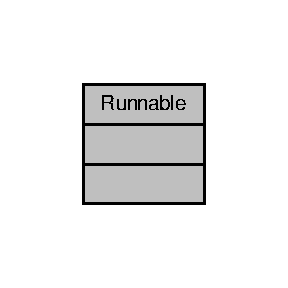
\includegraphics[width=138pt]{class_runnable__coll__graph}
\end{center}
\end{figure}


La documentation de cette classe a été générée à partir du fichier suivant \+:\begin{DoxyCompactItemize}
\item 
\hyperlink{_communication_8java}{Communication.\+java}\end{DoxyCompactItemize}

\hypertarget{classcom_1_1lasalle_1_1meeting_1_1_espace_de_travail_adaptateur_1_1_view_holder}{}\subsection{Référence de la classe com.\+lasalle.\+meeting.\+Espace\+De\+Travail\+Adaptateur.\+View\+Holder}
\label{classcom_1_1lasalle_1_1meeting_1_1_espace_de_travail_adaptateur_1_1_view_holder}\index{com.\+lasalle.\+meeting.\+Espace\+De\+Travail\+Adaptateur.\+View\+Holder@{com.\+lasalle.\+meeting.\+Espace\+De\+Travail\+Adaptateur.\+View\+Holder}}


Graphe de collaboration de com.\+lasalle.\+meeting.\+Espace\+De\+Travail\+Adaptateur.\+View\+Holder\+:\nopagebreak
\begin{figure}[H]
\begin{center}
\leavevmode
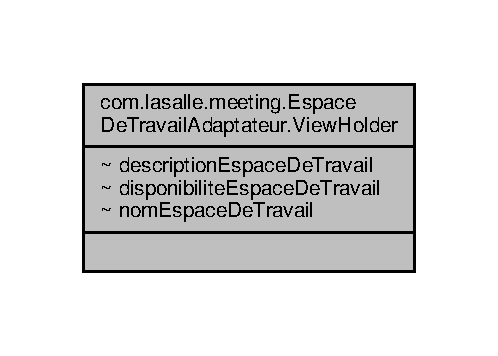
\includegraphics[width=239pt]{classcom_1_1lasalle_1_1meeting_1_1_espace_de_travail_adaptateur_1_1_view_holder__coll__graph}
\end{center}
\end{figure}


\subsubsection{Description détaillée}


Définition à la ligne \hyperlink{_espace_de_travail_adaptateur_8java_source_l00032}{32} du fichier \hyperlink{_espace_de_travail_adaptateur_8java_source}{Espace\+De\+Travail\+Adaptateur.\+java}.



La documentation de cette classe a été générée à partir du fichier suivant \+:\begin{DoxyCompactItemize}
\item 
\hyperlink{_espace_de_travail_adaptateur_8java}{Espace\+De\+Travail\+Adaptateur.\+java}\end{DoxyCompactItemize}

\section{Documentation des fichiers}
\hypertarget{_affichage_espace_de_travail_8java}{}\subsection{Référence du fichier Affichage\+Espace\+De\+Travail.\+java}
\label{_affichage_espace_de_travail_8java}\index{Affichage\+Espace\+De\+Travail.\+java@{Affichage\+Espace\+De\+Travail.\+java}}


Déclaration de la classe Affichage\+Espace\+De\+Travail.  


\subsubsection*{Classes}
\begin{DoxyCompactItemize}
\item 
class \hyperlink{classcom_1_1lasalle_1_1meeting_1_1_affichage_espace_de_travail}{com.\+lasalle.\+meeting.\+Affichage\+Espace\+De\+Travail}
\begin{DoxyCompactList}\small\item\em L\textquotesingle{}activité d\textquotesingle{}affichage d\textquotesingle{}un espace de travail de l\textquotesingle{}application Meeting. \end{DoxyCompactList}\end{DoxyCompactItemize}
\subsubsection*{Paquetages}
\begin{DoxyCompactItemize}
\item 
package \hyperlink{namespacecom_1_1lasalle_1_1meeting}{com.\+lasalle.\+meeting}
\end{DoxyCompactItemize}


\subsubsection{Description détaillée}
Déclaration de la classe Affichage\+Espace\+De\+Travail. 

\begin{DoxyAuthor}{Auteur}
K\+E\+L\+L\+E\+R-\/\+L\+A\+V\+A\+L\+L\+EE Joachim 
\end{DoxyAuthor}
\begin{DoxyParagraph}{Last\+Changed\+Revision}
46 
\end{DoxyParagraph}
\begin{DoxyParagraph}{Last\+Changed\+Date}
2021-\/04-\/27 21\+:25\+:45 +0200 (mar. 27 avril 2021) 
\end{DoxyParagraph}


Définition dans le fichier \hyperlink{_affichage_espace_de_travail_8java_source}{Affichage\+Espace\+De\+Travail.\+java}.


\hypertarget{_affichage_espace_de_travail_8java_source}{}\subsection{Affichage\+Espace\+De\+Travail.\+java}
\label{_affichage_espace_de_travail_8java_source}\index{Affichage\+Espace\+De\+Travail.\+java@{Affichage\+Espace\+De\+Travail.\+java}}

\begin{DoxyCode}
\Hypertarget{_affichage_espace_de_travail_8java_source_l00001}\hyperlink{namespacecom_1_1lasalle_1_1meeting}{00001} \textcolor{keyword}{package }com.lasalle.meeting;
00002 
00003 \textcolor{keyword}{import} androidx.appcompat.app.AppCompatActivity;
00004 
00005 \textcolor{keyword}{import} android.content.Intent;
00006 \textcolor{keyword}{import} android.graphics.Color;
00007 \textcolor{keyword}{import} android.os.Bundle;
00008 \textcolor{keyword}{import} android.util.Log;
00009 \textcolor{keyword}{import} android.view.View;
00010 \textcolor{keyword}{import} android.widget.TextView;
00011 \textcolor{keyword}{import} android.widget.Button;
00012 
\Hypertarget{_affichage_espace_de_travail_8java_source_l00025}\hyperlink{classcom_1_1lasalle_1_1meeting_1_1_affichage_espace_de_travail}{00025} \textcolor{keyword}{public} \textcolor{keyword}{class }\hyperlink{classcom_1_1lasalle_1_1meeting_1_1_affichage_espace_de_travail}{AffichageEspaceDeTravail} \textcolor{keyword}{extends} AppCompatActivity
00026 \{
\Hypertarget{_affichage_espace_de_travail_8java_source_l00030}\hyperlink{classcom_1_1lasalle_1_1meeting_1_1_affichage_espace_de_travail_a8606eb11c7b28f52226544de431d86a4}{00030}     \textcolor{keyword}{private} \textcolor{keyword}{static} \textcolor{keyword}{final} String \hyperlink{classcom_1_1lasalle_1_1meeting_1_1_affichage_espace_de_travail_a8606eb11c7b28f52226544de431d86a4}{TAG} = \textcolor{stringliteral}{"\_AffichageEspaceTravail"};
00031 
\Hypertarget{_affichage_espace_de_travail_8java_source_l00035}\hyperlink{classcom_1_1lasalle_1_1meeting_1_1_affichage_espace_de_travail_a934d41c1c41882b94b65a95cee5aca13}{00035}     \textcolor{keyword}{private} \hyperlink{classcom_1_1lasalle_1_1meeting_1_1_espace_de_travail}{EspaceDeTravail} \hyperlink{classcom_1_1lasalle_1_1meeting_1_1_affichage_espace_de_travail_a934d41c1c41882b94b65a95cee5aca13}{espaceDeTravail};
00036 
00040     @Override
\Hypertarget{_affichage_espace_de_travail_8java_source_l00041}\hyperlink{classcom_1_1lasalle_1_1meeting_1_1_affichage_espace_de_travail_a333ff077dde89888afc62366f6dccf06}{00041}     \textcolor{keyword}{protected} \textcolor{keywordtype}{void} \hyperlink{classcom_1_1lasalle_1_1meeting_1_1_affichage_espace_de_travail_a333ff077dde89888afc62366f6dccf06}{onCreate}(Bundle savedInstanceState)
00042     \{
00043         super.onCreate(savedInstanceState);
00044         setContentView(R.layout.activity\_affichage\_espace\_de\_travail);
00045         Intent intent = getIntent();
00046         espaceDeTravail = (\hyperlink{classcom_1_1lasalle_1_1meeting_1_1_espace_de_travail}{EspaceDeTravail})intent.getSerializableExtra(\textcolor{stringliteral}{"unEspaceDeTravail"});
00047 
00048         \hyperlink{classcom_1_1lasalle_1_1meeting_1_1_affichage_espace_de_travail_a62159c3fd69a3d4f03306bd3e75c09ce}{afficherNom}();
00049         \hyperlink{classcom_1_1lasalle_1_1meeting_1_1_affichage_espace_de_travail_a86fc32986ef9ae8f6ef7fca78d91f648}{afficherLieu}();
00050         \hyperlink{classcom_1_1lasalle_1_1meeting_1_1_affichage_espace_de_travail_a4afb30e3faf37f738f6261fc0696d62b}{afficherDescription}();
00051         \hyperlink{classcom_1_1lasalle_1_1meeting_1_1_affichage_espace_de_travail_ae8f1d5cb6d99aced1996b1b2bbcebe26}{afficherSuperficie}();
00052         \hyperlink{classcom_1_1lasalle_1_1meeting_1_1_affichage_espace_de_travail_a9474bdc380c78e632cc8d384d7393f50}{afficherTemperature}();
00053         \hyperlink{classcom_1_1lasalle_1_1meeting_1_1_affichage_espace_de_travail_acd704eb42f942a10a118d872ffe779a3}{afficherIndiceDeConfort}();
00054         \hyperlink{classcom_1_1lasalle_1_1meeting_1_1_affichage_espace_de_travail_a597703fc6f7e82b79ac7047640fa9323}{afficherDisponibilite}();
00055         \hyperlink{classcom_1_1lasalle_1_1meeting_1_1_affichage_espace_de_travail_a01e3d2585c84043dbe5086a2fc81c371}{afficherBoutonsReservation}();
00056     \}
00057 
\Hypertarget{_affichage_espace_de_travail_8java_source_l00061}\hyperlink{classcom_1_1lasalle_1_1meeting_1_1_affichage_espace_de_travail_a62159c3fd69a3d4f03306bd3e75c09ce}{00061}     \textcolor{keyword}{public} \textcolor{keywordtype}{void} \hyperlink{classcom_1_1lasalle_1_1meeting_1_1_affichage_espace_de_travail_a62159c3fd69a3d4f03306bd3e75c09ce}{afficherNom}()
00062     \{
00063         TextView affichageNom = (TextView)findViewById(R.id.affichageNom);
00064         affichageNom.setText(espaceDeTravail.\hyperlink{classcom_1_1lasalle_1_1meeting_1_1_espace_de_travail_ae662e2674616a8548755cb64a38e0432}{getNom}());
00065 
00066         Log.d(TAG, \textcolor{stringliteral}{"afficherNom() "} + espaceDeTravail.\hyperlink{classcom_1_1lasalle_1_1meeting_1_1_espace_de_travail_ae662e2674616a8548755cb64a38e0432}{getNom}());
00067     \}
00068 
\Hypertarget{_affichage_espace_de_travail_8java_source_l00072}\hyperlink{classcom_1_1lasalle_1_1meeting_1_1_affichage_espace_de_travail_a86fc32986ef9ae8f6ef7fca78d91f648}{00072}     \textcolor{keyword}{public} \textcolor{keywordtype}{void} \hyperlink{classcom_1_1lasalle_1_1meeting_1_1_affichage_espace_de_travail_a86fc32986ef9ae8f6ef7fca78d91f648}{afficherLieu}()
00073     \{
00074         TextView affichageLieu = (TextView)findViewById(R.id.affichageLieu);
00075         affichageLieu.setText(espaceDeTravail.\hyperlink{classcom_1_1lasalle_1_1meeting_1_1_espace_de_travail_af320aa4ad7711ed52b3b5aef1bd52dd1}{getLieu}());
00076 
00077         Log.d(TAG, \textcolor{stringliteral}{"afficherLieu() "} + espaceDeTravail.\hyperlink{classcom_1_1lasalle_1_1meeting_1_1_espace_de_travail_af320aa4ad7711ed52b3b5aef1bd52dd1}{getLieu}());
00078     \}
00079 
\Hypertarget{_affichage_espace_de_travail_8java_source_l00083}\hyperlink{classcom_1_1lasalle_1_1meeting_1_1_affichage_espace_de_travail_a4afb30e3faf37f738f6261fc0696d62b}{00083}     \textcolor{keyword}{public} \textcolor{keywordtype}{void} \hyperlink{classcom_1_1lasalle_1_1meeting_1_1_affichage_espace_de_travail_a4afb30e3faf37f738f6261fc0696d62b}{afficherDescription}()
00084     \{
00085         TextView affichageDescription = (TextView)findViewById(R.id.affichageDescription);
00086         affichageDescription.setText(espaceDeTravail.\hyperlink{classcom_1_1lasalle_1_1meeting_1_1_espace_de_travail_a815ecee3f01117f2d9b1d9441b214907}{getDescription}());
00087 
00088         Log.d(TAG, \textcolor{stringliteral}{"afficherDescription() "} + espaceDeTravail.\hyperlink{classcom_1_1lasalle_1_1meeting_1_1_espace_de_travail_a815ecee3f01117f2d9b1d9441b214907}{getDescription}());
00089     \}
00090 
\Hypertarget{_affichage_espace_de_travail_8java_source_l00094}\hyperlink{classcom_1_1lasalle_1_1meeting_1_1_affichage_espace_de_travail_ae8f1d5cb6d99aced1996b1b2bbcebe26}{00094}     \textcolor{keyword}{public} \textcolor{keywordtype}{void} \hyperlink{classcom_1_1lasalle_1_1meeting_1_1_affichage_espace_de_travail_ae8f1d5cb6d99aced1996b1b2bbcebe26}{afficherSuperficie}()
00095     \{
00096         TextView affichageSuperficie = (TextView)findViewById(R.id.affichageSuperficie);
00097         affichageSuperficie.setText(String.valueOf(espaceDeTravail.\hyperlink{classcom_1_1lasalle_1_1meeting_1_1_espace_de_travail_ae2c734da9d454b368ddb056b1cdae499}{getSuperficie}()));
00098 
00099         Log.d(TAG, \textcolor{stringliteral}{"afficherSuperficie() "} + espaceDeTravail.\hyperlink{classcom_1_1lasalle_1_1meeting_1_1_espace_de_travail_ae2c734da9d454b368ddb056b1cdae499}{getSuperficie}());
00100     \}
00101 
\Hypertarget{_affichage_espace_de_travail_8java_source_l00105}\hyperlink{classcom_1_1lasalle_1_1meeting_1_1_affichage_espace_de_travail_a9474bdc380c78e632cc8d384d7393f50}{00105}     \textcolor{keyword}{public} \textcolor{keywordtype}{void} \hyperlink{classcom_1_1lasalle_1_1meeting_1_1_affichage_espace_de_travail_a9474bdc380c78e632cc8d384d7393f50}{afficherTemperature}()
00106     \{
00107         TextView affichageTemperature = (TextView)findViewById(R.id.affichageTemperature);
00108         affichageTemperature.setText(String.valueOf(espaceDeTravail.
      \hyperlink{classcom_1_1lasalle_1_1meeting_1_1_espace_de_travail_a4c01c37fa6431d48c59274aaa00fdbe3}{getTemperature}()));
00109 
00110         Log.d(TAG, \textcolor{stringliteral}{"afficherTemperature() "} + espaceDeTravail.\hyperlink{classcom_1_1lasalle_1_1meeting_1_1_espace_de_travail_a4c01c37fa6431d48c59274aaa00fdbe3}{getTemperature}());
00111     \}
00112 
\Hypertarget{_affichage_espace_de_travail_8java_source_l00116}\hyperlink{classcom_1_1lasalle_1_1meeting_1_1_affichage_espace_de_travail_acd704eb42f942a10a118d872ffe779a3}{00116}     \textcolor{keyword}{public} \textcolor{keywordtype}{void} \hyperlink{classcom_1_1lasalle_1_1meeting_1_1_affichage_espace_de_travail_acd704eb42f942a10a118d872ffe779a3}{afficherIndiceDeConfort}()
00117     \{
00118         TextView affichageIndiceDeConfort = (TextView)findViewById(R.id.affichageIndiceDeConfort);
00119         affichageIndiceDeConfort.setText(String.valueOf(espaceDeTravail.
      \hyperlink{classcom_1_1lasalle_1_1meeting_1_1_espace_de_travail_a9d7b3bd8aa78a10c70851b477d0f522d}{getIndiceDeConfort}()));
00120 
00121         Log.d(TAG, \textcolor{stringliteral}{"afficherIndiceDeConfort() "} + espaceDeTravail.
      \hyperlink{classcom_1_1lasalle_1_1meeting_1_1_espace_de_travail_a9d7b3bd8aa78a10c70851b477d0f522d}{getIndiceDeConfort}());
00122     \}
00123 
\Hypertarget{_affichage_espace_de_travail_8java_source_l00127}\hyperlink{classcom_1_1lasalle_1_1meeting_1_1_affichage_espace_de_travail_a597703fc6f7e82b79ac7047640fa9323}{00127}     \textcolor{keyword}{public} \textcolor{keywordtype}{void} \hyperlink{classcom_1_1lasalle_1_1meeting_1_1_affichage_espace_de_travail_a597703fc6f7e82b79ac7047640fa9323}{afficherDisponibilite}()
00128     \{
00129         TextView affichageDisponibilite = (TextView)findViewById(R.id.affichageDisponibilite);
00130 
00131         \textcolor{keywordflow}{if}(!espaceDeTravail.\hyperlink{classcom_1_1lasalle_1_1meeting_1_1_espace_de_travail_a69fe30f8d3aff92986f4c39402e16ab0}{getEstReserve}())
00132         \{
00133             Log.d(TAG, \textcolor{stringliteral}{"Libre"});
00134             affichageDisponibilite.setText(\textcolor{stringliteral}{"Libre"});
00135             affichageDisponibilite.setTextColor(Color.parseColor(\textcolor{stringliteral}{"#00FF00"})); \textcolor{comment}{// Color.rgb(0,255,0)}
00136         \}
00137         \textcolor{keywordflow}{else}
00138         \{
00139             Log.d(TAG, \textcolor{stringliteral}{"Occupé"});
00140             affichageDisponibilite.setText(\textcolor{stringliteral}{"Occupé"});
00141             affichageDisponibilite.setTextColor(Color.rgb(255,0,0));
00142         \}
00143 
00144         Log.d(TAG, \textcolor{stringliteral}{"afficherDisponibilite() "} + espaceDeTravail.\hyperlink{classcom_1_1lasalle_1_1meeting_1_1_espace_de_travail_a69fe30f8d3aff92986f4c39402e16ab0}{getEstReserve}());
00145     \}
00146 
\Hypertarget{_affichage_espace_de_travail_8java_source_l00150}\hyperlink{classcom_1_1lasalle_1_1meeting_1_1_affichage_espace_de_travail_a01e3d2585c84043dbe5086a2fc81c371}{00150}     \textcolor{keyword}{public} \textcolor{keywordtype}{void} \hyperlink{classcom_1_1lasalle_1_1meeting_1_1_affichage_espace_de_travail_a01e3d2585c84043dbe5086a2fc81c371}{afficherBoutonsReservation}()
00151     \{
00152         Button boutonReserver = (Button)findViewById(R.id.boutonReserver);
00153         Button boutonLiberer = (Button)findViewById(R.id.boutonLiberer);
00154 
00155         boutonReserver.setOnClickListener(
00156                 \textcolor{keyword}{new} View.OnClickListener()
00157                 \{
00158                     \textcolor{keyword}{public} \textcolor{keywordtype}{void} onClick(View v)
00159                     \{
00160                         espaceDeTravail.\hyperlink{classcom_1_1lasalle_1_1meeting_1_1_espace_de_travail_a42d483a68e6d0d50707dbd3dddd164c2}{reserver}();
00161                         \hyperlink{classcom_1_1lasalle_1_1meeting_1_1_affichage_espace_de_travail_a597703fc6f7e82b79ac7047640fa9323}{afficherDisponibilite}();
00162                         \hyperlink{classcom_1_1lasalle_1_1meeting_1_1_affichage_espace_de_travail_a01e3d2585c84043dbe5086a2fc81c371}{afficherBoutonsReservation}();
00163                     \}
00164                 \}
00165         );
00166 
00167         boutonLiberer.setOnClickListener(
00168                 \textcolor{keyword}{new} View.OnClickListener()
00169                 \{
00170                     \textcolor{keyword}{public} \textcolor{keywordtype}{void} onClick(View v)
00171                     \{
00172                         espaceDeTravail.\hyperlink{classcom_1_1lasalle_1_1meeting_1_1_espace_de_travail_affce017a0a5ba338d7b0b7f6bbce6c68}{liberer}();
00173                         \hyperlink{classcom_1_1lasalle_1_1meeting_1_1_affichage_espace_de_travail_a597703fc6f7e82b79ac7047640fa9323}{afficherDisponibilite}();
00174                         \hyperlink{classcom_1_1lasalle_1_1meeting_1_1_affichage_espace_de_travail_a01e3d2585c84043dbe5086a2fc81c371}{afficherBoutonsReservation}();
00175                     \}
00176                 \}
00177         );
00178 
00179         \textcolor{keywordflow}{if}(!espaceDeTravail.\hyperlink{classcom_1_1lasalle_1_1meeting_1_1_espace_de_travail_a69fe30f8d3aff92986f4c39402e16ab0}{getEstReserve}())
00180         \{
00181             boutonReserver.setVisibility(View.VISIBLE);
00182             boutonLiberer.setVisibility(View.GONE);
00183         \}
00184         \textcolor{keywordflow}{else}
00185         \{
00186             boutonReserver.setVisibility(View.GONE);
00187             boutonLiberer.setVisibility(View.VISIBLE);
00188         \}
00189     \}
00190 
00194     @Override
\Hypertarget{_affichage_espace_de_travail_8java_source_l00195}\hyperlink{classcom_1_1lasalle_1_1meeting_1_1_affichage_espace_de_travail_a2f3649336aff1f2126f817c72faf30c2}{00195}     \textcolor{keyword}{public} \textcolor{keywordtype}{void} \hyperlink{classcom_1_1lasalle_1_1meeting_1_1_affichage_espace_de_travail_a2f3649336aff1f2126f817c72faf30c2}{finish}()
00196     \{
00197         Log.d(TAG, \textcolor{stringliteral}{"finish()"});
00198 
00199         Intent intent = \textcolor{keyword}{new} Intent();
00200         intent.putExtra(\textcolor{stringliteral}{"unEspaceDeTravail"}, espaceDeTravail);
00201 
00202         setResult(RESULT\_OK, intent);
00203         super.finish();
00204     \}
00205 \}
\end{DoxyCode}

\hypertarget{_communication_8java}{}\subsection{Référence du fichier Communication.\+java}
\label{_communication_8java}\index{Communication.\+java@{Communication.\+java}}


Déclaration de la classe Communication.  


\subsubsection*{Classes}
\begin{DoxyCompactItemize}
\item 
class \hyperlink{classcom_1_1lasalle_1_1meeting_1_1_communication}{com.\+lasalle.\+meeting.\+Communication}
\begin{DoxyCompactList}\small\item\em \hyperlink{classcom_1_1lasalle_1_1meeting_1_1_communication}{Communication} entre l\textquotesingle{}application et le portier. \end{DoxyCompactList}\end{DoxyCompactItemize}
\subsubsection*{Paquetages}
\begin{DoxyCompactItemize}
\item 
package \hyperlink{namespacecom_1_1lasalle_1_1meeting}{com.\+lasalle.\+meeting}
\end{DoxyCompactItemize}


\subsubsection{Description détaillée}
Déclaration de la classe Communication. 

\begin{DoxyAuthor}{Auteur}
K\+E\+L\+L\+E\+R-\/\+L\+A\+V\+A\+L\+L\+EE Joachim 
\end{DoxyAuthor}
\begin{DoxyParagraph}{Last\+Changed\+Revision}
46 
\end{DoxyParagraph}
\begin{DoxyParagraph}{Last\+Changed\+Date}
2021-\/04-\/27 21\+:25\+:45 +0200 (mar. 27 avril 2021) 
\end{DoxyParagraph}


Définition dans le fichier \hyperlink{_communication_8java_source}{Communication.\+java}.


\hypertarget{_communication_8java_source}{}\subsection{Communication.\+java}
\label{_communication_8java_source}\index{Communication.\+java@{Communication.\+java}}

\begin{DoxyCode}
00001 \textcolor{keyword}{package }com.lasalle.meeting;
00002 
00003 \textcolor{keyword}{import} android.os.Bundle;
00004 \textcolor{keyword}{import} android.os.Handler;
00005 \textcolor{keyword}{import} android.os.Message;
00006 \textcolor{keyword}{import} android.util.Log;
00007 
00008 \textcolor{keyword}{import} java.io.IOException;
00009 \textcolor{keyword}{import} java.net.DatagramPacket;
00010 \textcolor{keyword}{import} java.net.DatagramSocket;
00011 \textcolor{keyword}{import} java.net.InetAddress;
00012 \textcolor{keyword}{import} java.net.UnknownHostException;
00013 \textcolor{keyword}{import} java.util.List;
00014 \textcolor{keyword}{import} java.util.concurrent.LinkedBlockingQueue;
00015 \textcolor{keyword}{import} java.util.concurrent.locks.ReentrantLock;
00016 
\Hypertarget{_communication_8java_source_l00029}\hyperlink{classcom_1_1lasalle_1_1meeting_1_1_communication}{00029} \textcolor{keyword}{public} \textcolor{keyword}{class }\hyperlink{classcom_1_1lasalle_1_1meeting_1_1_communication}{Communication} \textcolor{keyword}{implements} \hyperlink{class_runnable}{Runnable}
00030 \{
\Hypertarget{_communication_8java_source_l00034}\hyperlink{classcom_1_1lasalle_1_1meeting_1_1_communication_a5d58f88df1f20b4d61edbed9a82eccab}{00034}     \textcolor{keyword}{private} \textcolor{keyword}{static} \textcolor{keyword}{final} String \hyperlink{classcom_1_1lasalle_1_1meeting_1_1_communication_a5d58f88df1f20b4d61edbed9a82eccab}{TAG} = \textcolor{stringliteral}{"\_Communication"};
00035 
\Hypertarget{_communication_8java_source_l00039}\hyperlink{classcom_1_1lasalle_1_1meeting_1_1_communication_a46e5fbc8ec97ad651d544e09121a6468}{00039}     \textcolor{keyword}{private} InetAddress \hyperlink{classcom_1_1lasalle_1_1meeting_1_1_communication_a46e5fbc8ec97ad651d544e09121a6468}{adresseIP} = null;
\Hypertarget{_communication_8java_source_l00040}\hyperlink{classcom_1_1lasalle_1_1meeting_1_1_communication_a6a2d2e62f87bef261a1999eb5acf8abb}{00040}     \textcolor{keyword}{public} \textcolor{keyword}{final} \textcolor{keyword}{static} String \hyperlink{classcom_1_1lasalle_1_1meeting_1_1_communication_a6a2d2e62f87bef261a1999eb5acf8abb}{adresseMulticast} = \textcolor{stringliteral}{"239.0.0.42"};    
\Hypertarget{_communication_8java_source_l00041}\hyperlink{classcom_1_1lasalle_1_1meeting_1_1_communication_abf48fd6a29d87d67f4941494404f1ea7}{00041}     \textcolor{keyword}{private} \textcolor{keyword}{final} \textcolor{keyword}{static} \textcolor{keywordtype}{int} \hyperlink{classcom_1_1lasalle_1_1meeting_1_1_communication_abf48fd6a29d87d67f4941494404f1ea7}{PORT} = 5000;                           
\Hypertarget{_communication_8java_source_l00042}\hyperlink{classcom_1_1lasalle_1_1meeting_1_1_communication_a4997d801f57344fb4eea7924903c2d6c}{00042}     \textcolor{keyword}{public} \textcolor{keyword}{final} \textcolor{keyword}{static} \textcolor{keywordtype}{int} \hyperlink{classcom_1_1lasalle_1_1meeting_1_1_communication_a4997d801f57344fb4eea7924903c2d6c}{TYPE\_RECEPTION} = 1;                     
\Hypertarget{_communication_8java_source_l00043}\hyperlink{classcom_1_1lasalle_1_1meeting_1_1_communication_af123afba8dcddc259017fb5c3b431dab}{00043}     \textcolor{keyword}{private} \textcolor{keyword}{final} ReentrantLock \hyperlink{classcom_1_1lasalle_1_1meeting_1_1_communication_af123afba8dcddc259017fb5c3b431dab}{mutex} = \textcolor{keyword}{new} ReentrantLock();
\Hypertarget{_communication_8java_source_l00044}\hyperlink{classcom_1_1lasalle_1_1meeting_1_1_communication_a2a538f36640aecebbb833bbaf1f03858}{00044}     \textcolor{keyword}{private} DatagramSocket \hyperlink{classcom_1_1lasalle_1_1meeting_1_1_communication_a2a538f36640aecebbb833bbaf1f03858}{socket} = null;
\Hypertarget{_communication_8java_source_l00045}\hyperlink{classcom_1_1lasalle_1_1meeting_1_1_communication_a733017de1be51e6e6ebf6719009ede30}{00045}     \textcolor{keyword}{private} LinkedBlockingQueue<DatagramPacket> \hyperlink{classcom_1_1lasalle_1_1meeting_1_1_communication_a733017de1be51e6e6ebf6719009ede30}{queueEmission};
\Hypertarget{_communication_8java_source_l00046}\hyperlink{classcom_1_1lasalle_1_1meeting_1_1_communication_a05fa5f360f28819a9e106e0265a74643}{00046}     \textcolor{keyword}{private} Handler \hyperlink{classcom_1_1lasalle_1_1meeting_1_1_communication_a05fa5f360f28819a9e106e0265a74643}{handler};                        
00047 
\Hypertarget{_communication_8java_source_l00051}\hyperlink{classcom_1_1lasalle_1_1meeting_1_1_communication_a6560c39bb7ebc968e007e4dd98ec296c}{00051}     \textcolor{keyword}{public} \textcolor{keyword}{static} \textcolor{keyword}{final} String \hyperlink{classcom_1_1lasalle_1_1meeting_1_1_communication_a6560c39bb7ebc968e007e4dd98ec296c}{DELIMITEUR\_EN\_TETE} = \textcolor{stringliteral}{"$"};
\Hypertarget{_communication_8java_source_l00052}\hyperlink{classcom_1_1lasalle_1_1meeting_1_1_communication_aeff38852b1f770d9a13cd5bf02090bb1}{00052}     \textcolor{keyword}{public} \textcolor{keyword}{static} \textcolor{keyword}{final} String \hyperlink{classcom_1_1lasalle_1_1meeting_1_1_communication_aeff38852b1f770d9a13cd5bf02090bb1}{DELIMITEUR\_CHAMP} = \textcolor{stringliteral}{";"};
\Hypertarget{_communication_8java_source_l00053}\hyperlink{classcom_1_1lasalle_1_1meeting_1_1_communication_a6f2e7cb2145496069cdf1b33d017be58}{00053}     \textcolor{keyword}{public} \textcolor{keyword}{static} \textcolor{keyword}{final} String \hyperlink{classcom_1_1lasalle_1_1meeting_1_1_communication_a6f2e7cb2145496069cdf1b33d017be58}{DELIMITEUR\_FIN} = \textcolor{stringliteral}{"\(\backslash\)r\(\backslash\)n"};
\Hypertarget{_communication_8java_source_l00054}\hyperlink{classcom_1_1lasalle_1_1meeting_1_1_communication_a9a0b852b1753e97242edaba93f63a4d6}{00054}     \textcolor{keyword}{public} \textcolor{keyword}{static} \textcolor{keyword}{final} \textcolor{keywordtype}{int} \hyperlink{classcom_1_1lasalle_1_1meeting_1_1_communication_a9a0b852b1753e97242edaba93f63a4d6}{DEMANDE\_INFORMATIONS} = 1;
\Hypertarget{_communication_8java_source_l00055}\hyperlink{classcom_1_1lasalle_1_1meeting_1_1_communication_acb13915d9514b99c3b9bc99358e42db6}{00055}     \textcolor{keyword}{public} \textcolor{keyword}{static} \textcolor{keyword}{final} \textcolor{keywordtype}{int} \hyperlink{classcom_1_1lasalle_1_1meeting_1_1_communication_acb13915d9514b99c3b9bc99358e42db6}{DEMANDE\_ETAT} = 2;
\Hypertarget{_communication_8java_source_l00056}\hyperlink{classcom_1_1lasalle_1_1meeting_1_1_communication_a518dd253a20818a8bbc672ffcd93aeb7}{00056}     \textcolor{keyword}{public} \textcolor{keyword}{static} \textcolor{keyword}{final} \textcolor{keywordtype}{int} \hyperlink{classcom_1_1lasalle_1_1meeting_1_1_communication_a518dd253a20818a8bbc672ffcd93aeb7}{DEMANDE\_DISPONIBILITE} = 3;
\Hypertarget{_communication_8java_source_l00057}\hyperlink{classcom_1_1lasalle_1_1meeting_1_1_communication_ad982608d86bb6b724bf9289592b7945b}{00057}     \textcolor{keyword}{public} \textcolor{keyword}{static} \textcolor{keyword}{final} \textcolor{keywordtype}{int} \hyperlink{classcom_1_1lasalle_1_1meeting_1_1_communication_ad982608d86bb6b724bf9289592b7945b}{MODIFICATION\_INFORMATIONS} = 1;
\Hypertarget{_communication_8java_source_l00058}\hyperlink{classcom_1_1lasalle_1_1meeting_1_1_communication_a39defd6718a8774ae75addf9f8f6f3cd}{00058}     \textcolor{keyword}{public} \textcolor{keyword}{static} \textcolor{keyword}{final} \textcolor{keywordtype}{int} \hyperlink{classcom_1_1lasalle_1_1meeting_1_1_communication_a39defd6718a8774ae75addf9f8f6f3cd}{MODIFICATION\_DISPONIBILITE} = 3;
\Hypertarget{_communication_8java_source_l00059}\hyperlink{classcom_1_1lasalle_1_1meeting_1_1_communication_af9211740f83da963f0c4ea84b84f0669}{00059}     \textcolor{keyword}{public} \textcolor{keyword}{static} \textcolor{keyword}{final} \textcolor{keywordtype}{int} \hyperlink{classcom_1_1lasalle_1_1meeting_1_1_communication_af9211740f83da963f0c4ea84b84f0669}{NB\_CHAMPS\_INFORMATIONS} = 4;
\Hypertarget{_communication_8java_source_l00060}\hyperlink{classcom_1_1lasalle_1_1meeting_1_1_communication_a9c88b5b4215e040b3928f6c01914bfa7}{00060}     \textcolor{keyword}{public} \textcolor{keyword}{static} \textcolor{keyword}{final} \textcolor{keywordtype}{int} \hyperlink{classcom_1_1lasalle_1_1meeting_1_1_communication_a9c88b5b4215e040b3928f6c01914bfa7}{NB\_CHAMPS\_DISPONIBILITE} = 1;
\Hypertarget{_communication_8java_source_l00061}\hyperlink{classcom_1_1lasalle_1_1meeting_1_1_communication_a8e064e494a3d43ced5aefb524701bc22}{00061}     \textcolor{keyword}{public} \textcolor{keyword}{static} \textcolor{keyword}{final} \textcolor{keywordtype}{int} \hyperlink{classcom_1_1lasalle_1_1meeting_1_1_communication_a8e064e494a3d43ced5aefb524701bc22}{CHAMP\_NOM} = 0;
\Hypertarget{_communication_8java_source_l00062}\hyperlink{classcom_1_1lasalle_1_1meeting_1_1_communication_ab1b74caade66cc37a1180d3f10383db8}{00062}     \textcolor{keyword}{public} \textcolor{keyword}{static} \textcolor{keyword}{final} \textcolor{keywordtype}{int} \hyperlink{classcom_1_1lasalle_1_1meeting_1_1_communication_ab1b74caade66cc37a1180d3f10383db8}{CHAMP\_DESCRIPTION} = 1;
\Hypertarget{_communication_8java_source_l00063}\hyperlink{classcom_1_1lasalle_1_1meeting_1_1_communication_a6f8e3d2386521c64c50eaa037083be79}{00063}     \textcolor{keyword}{private} \textcolor{keyword}{static} \textcolor{keyword}{final} \textcolor{keywordtype}{int} \hyperlink{classcom_1_1lasalle_1_1meeting_1_1_communication_a6f8e3d2386521c64c50eaa037083be79}{CHAMP\_LIEU} = 2;
\Hypertarget{_communication_8java_source_l00064}\hyperlink{classcom_1_1lasalle_1_1meeting_1_1_communication_a6f16e8be300ba2c9b2d3973f8da79942}{00064}     \textcolor{keyword}{private} \textcolor{keyword}{static} \textcolor{keyword}{final} \textcolor{keywordtype}{int} \hyperlink{classcom_1_1lasalle_1_1meeting_1_1_communication_a6f16e8be300ba2c9b2d3973f8da79942}{CHAMP\_SUPERFICIE} = 3;
00065 
\Hypertarget{_communication_8java_source_l00070}\hyperlink{classcom_1_1lasalle_1_1meeting_1_1_communication_a3d73554b2774d3274ad385b0faa27d14}{00070}     \textcolor{keyword}{public} \hyperlink{classcom_1_1lasalle_1_1meeting_1_1_communication_a3d73554b2774d3274ad385b0faa27d14}{Communication}(Handler handler)
00071     \{
00072         this.handler = \hyperlink{classcom_1_1lasalle_1_1meeting_1_1_communication_a05fa5f360f28819a9e106e0265a74643}{handler};
00073 
00074         \textcolor{keywordflow}{try}
00075         \{
00076             socket = \textcolor{keyword}{new} DatagramSocket(PORT);
00077             Log.d(TAG, \textcolor{stringliteral}{"Création de la socket UDP sur le port "} + PORT);
00078         \}
00079         \textcolor{keywordflow}{catch}(Exception e)
00080         \{
00081             e.printStackTrace();
00082         \}
00083 
00084         queueEmission = \textcolor{keyword}{new} LinkedBlockingQueue<DatagramPacket>();
00085     \}
00086 
\Hypertarget{_communication_8java_source_l00090}\hyperlink{classcom_1_1lasalle_1_1meeting_1_1_communication_a03f0e419513d7f33900dde412e2a4471}{00090}     \textcolor{keyword}{public} \textcolor{keywordtype}{void} \hyperlink{classcom_1_1lasalle_1_1meeting_1_1_communication_a03f0e419513d7f33900dde412e2a4471}{envoyer}(String trame, String adressePortier)
00091     \{
00092         \textcolor{keywordflow}{if}(socket == null || socket.isClosed())
00093             \textcolor{keywordflow}{return};
00094 
00095         \textcolor{keyword}{final} InetAddress adresseIPDistante;
00096         \textcolor{keywordflow}{try}
00097         \{
00098             adresseIPDistante = InetAddress.getByName(adressePortier);
00099         \}
00100         \textcolor{keywordflow}{catch} (UnknownHostException e)
00101         \{
00102             e.printStackTrace();
00103             \textcolor{keywordflow}{return};
00104         \}
00105 
00106         \textcolor{comment}{// Crée et démarre un thread pour envoyer la trame}
00107         \textcolor{keyword}{new} Thread()
00108         \{
00109             @Override \textcolor{keyword}{public} \textcolor{keywordtype}{void} \hyperlink{classcom_1_1lasalle_1_1meeting_1_1_communication_afe29bde1b4538990bd0a8c9b2d512efa}{run}()
00110             \{
00111                 byte[] emission = \textcolor{keyword}{new} byte[1024];
00112 
00113                 \textcolor{keywordflow}{try}
00114                 \{
00115                     emission = trame.getBytes();
00116                     DatagramPacket paquetRetour = \textcolor{keyword}{new} DatagramPacket(emission, emission.length, 
      adresseIPDistante, PORT);
00117                     socket.send(paquetRetour);
00118                     Log.d(TAG, \textcolor{stringliteral}{"envoyer()"} + trame);
00119                 \}
00120                 \textcolor{keywordflow}{catch} (IOException e)
00121                 \{
00122                     e.printStackTrace();
00123                     Log.d(TAG, \textcolor{stringliteral}{"Erreur émission !"});
00124                 \}
00125             \}
00126         \}.start();
00127     \}
00128 
\Hypertarget{_communication_8java_source_l00132}\hyperlink{classcom_1_1lasalle_1_1meeting_1_1_communication_a0344b79faa04dded3468fb8dda6baa81}{00132}     \textcolor{keyword}{public} \textcolor{keywordtype}{void} \hyperlink{classcom_1_1lasalle_1_1meeting_1_1_communication_a0344b79faa04dded3468fb8dda6baa81}{recevoir}()
00133     \{
00134         byte[] reception = \textcolor{keyword}{new} byte[1024];
00135 
00136         \textcolor{keywordflow}{while} (socket != null && !socket.isClosed())
00137         \{
00138             \textcolor{keywordflow}{try}
00139             \{
00140                 \textcolor{keyword}{final} DatagramPacket paquetRecu = \textcolor{keyword}{new} DatagramPacket(reception, reception.length);
00141                 socket.receive(paquetRecu);
00142                 \textcolor{keyword}{final} String donnees = \textcolor{keyword}{new} String(paquetRecu.getData(), paquetRecu.getOffset(), paquetRecu.
      getLength());
00143                 Log.d(TAG, \textcolor{stringliteral}{"Réception ["} + paquetRecu.getAddress().getHostAddress() + \textcolor{stringliteral}{":"} + paquetRecu.
      getPort() + \textcolor{stringliteral}{"] -> "} + donnees);
00144 
00145                 \textcolor{keywordflow}{if}(\hyperlink{classcom_1_1lasalle_1_1meeting_1_1_communication_af3090814ffb2fc9537961be52ebd17c2}{verifierTrame}(donnees))
00146                 \{
00147                     \textcolor{comment}{// Envoie les données reçues à l'activité}
00148                     \hyperlink{classcom_1_1lasalle_1_1meeting_1_1_communication_a7fa206969cf5dc48f4660845bbff0fc1}{envoyerMessage}(TYPE\_RECEPTION, paquetRecu.getAddress().getHostAddress(), 
      paquetRecu.getPort(), donnees);
00149                 \}
00150             \}
00151             \textcolor{keywordflow}{catch} (Exception e)
00152             \{
00153                 e.printStackTrace();
00154                 Log.d(TAG, \textcolor{stringliteral}{"Erreur réception !"});
00155             \}
00156         \}
00157 
00158         Log.d(TAG, \textcolor{stringliteral}{"recevoir()"});
00159     \}
00160 
\Hypertarget{_communication_8java_source_l00161}\hyperlink{classcom_1_1lasalle_1_1meeting_1_1_communication_a7fa206969cf5dc48f4660845bbff0fc1}{00161}     \textcolor{keyword}{private} \textcolor{keywordtype}{void} \hyperlink{classcom_1_1lasalle_1_1meeting_1_1_communication_a7fa206969cf5dc48f4660845bbff0fc1}{envoyerMessage}(\textcolor{keywordtype}{int} type, String adresse, \textcolor{keywordtype}{int} port, String donnees)
00162     \{
00163         Message msg = Message.obtain();
00164         msg.what = type;
00165         Bundle b = \textcolor{keyword}{new} Bundle();
00166         b.putString(\textcolor{stringliteral}{"adresseIP"}, adresse);
00167         b.putInt(\textcolor{stringliteral}{"port"}, port);
00168         b.putString(\textcolor{stringliteral}{"donnees"}, donnees);
00169         msg.setData(b);
00170         mutex.lock();
00171         handler.sendMessage(msg);
00172         mutex.unlock();
00173     \}
00174 
\Hypertarget{_communication_8java_source_l00180}\hyperlink{classcom_1_1lasalle_1_1meeting_1_1_communication_a3b07023cb3f3a1549da711b5c6ba6af1}{00180}     \textcolor{keyword}{public} String \hyperlink{classcom_1_1lasalle_1_1meeting_1_1_communication_a3b07023cb3f3a1549da711b5c6ba6af1}{fabriquerTrameDemande}(\textcolor{keywordtype}{int} typeTrame)
00181     \{
00182         \textcolor{comment}{/*}
00183 \textcolor{comment}{         * Protocole}
00184 \textcolor{comment}{         *}
00185 \textcolor{comment}{         * Demande informations du portier :}
00186 \textcolor{comment}{         * $GET;1\(\backslash\)r\(\backslash\)n}
00187 \textcolor{comment}{         *}
00188 \textcolor{comment}{         * Demande état du portier :}
00189 \textcolor{comment}{         * $GET;2\(\backslash\)r\(\backslash\)n}
00190 \textcolor{comment}{         *}
00191 \textcolor{comment}{         * Demande disponibilité du portier :}
00192 \textcolor{comment}{         * $GET;3\(\backslash\)r\(\backslash\)n}
00193 \textcolor{comment}{         *}
00194 \textcolor{comment}{         */}
00195 
00196         String trame = null;
00197         Log.d(TAG, \textcolor{stringliteral}{"fabriquerTrameDemande() type = "} + typeTrame);
00198 
00199         \textcolor{keywordflow}{switch}(typeTrame)
00200         \{
00201             \textcolor{keywordflow}{case} \hyperlink{classcom_1_1lasalle_1_1meeting_1_1_communication_a9a0b852b1753e97242edaba93f63a4d6}{DEMANDE\_INFORMATIONS}:
00202                 trame = \textcolor{stringliteral}{"$GET;1\(\backslash\)r\(\backslash\)n"};
00203                 \textcolor{keywordflow}{break};
00204             \textcolor{keywordflow}{case} \hyperlink{classcom_1_1lasalle_1_1meeting_1_1_communication_acb13915d9514b99c3b9bc99358e42db6}{DEMANDE\_ETAT}:
00205                 trame = \textcolor{stringliteral}{"$GET;2\(\backslash\)r\(\backslash\)n"};
00206                 \textcolor{keywordflow}{break};
00207             \textcolor{keywordflow}{case} \hyperlink{classcom_1_1lasalle_1_1meeting_1_1_communication_a518dd253a20818a8bbc672ffcd93aeb7}{DEMANDE\_DISPONIBILITE}:
00208                 trame = \textcolor{stringliteral}{"$GET;3\(\backslash\)r\(\backslash\)n"};
00209                 \textcolor{keywordflow}{break};
00210             \textcolor{keywordflow}{default}:
00211                 Log.d(TAG, \textcolor{stringliteral}{"fabriquerTrameDemande() : type de trame inconnu !"});
00212         \}
00213 
00214         \textcolor{keywordflow}{return} trame;
00215     \}
00216 
\Hypertarget{_communication_8java_source_l00222}\hyperlink{classcom_1_1lasalle_1_1meeting_1_1_communication_a82b49090e24d8296bfd26a14e0951ade}{00222}     \textcolor{keyword}{public} String \hyperlink{classcom_1_1lasalle_1_1meeting_1_1_communication_a82b49090e24d8296bfd26a14e0951ade}{fabriquerTrameModification}(\textcolor{keywordtype}{int} typeTrame, List<String> 
      parametres)
00223     \{
00224         \textcolor{comment}{/*}
00225 \textcolor{comment}{         * Protocole}
00226 \textcolor{comment}{         *}
00227 \textcolor{comment}{         * Actualiser les informations d’un portier :}
00228 \textcolor{comment}{         * $SET;1;nomSalle;description;emplacement;surface\(\backslash\)r\(\backslash\)n}
00229 \textcolor{comment}{         *}
00230 \textcolor{comment}{         * Actualiser la disponibilité d’un portier :}
00231 \textcolor{comment}{         * $SET;3;disponibilité\(\backslash\)r\(\backslash\)n}
00232 \textcolor{comment}{         *}
00233 \textcolor{comment}{         * Exemple d'utilisation :}
00234 \textcolor{comment}{         *   List<String> parametres = Arrays.asList("B11", "Salle de cours", "Batiment BTS", "25");}
00235 \textcolor{comment}{         *   String trame =
       communication.fabriquerTrameModification(Communication.MODIFICATION\_INFORMATIONS, parametres);}
00236 \textcolor{comment}{         */}
00237 
00238         \textcolor{comment}{// Vérifications}
00239         \textcolor{keywordflow}{if}(parametres == null)
00240             \textcolor{keywordflow}{return} null;
00241 
00242         \textcolor{keywordflow}{if}(parametres.size() != NB\_CHAMPS\_INFORMATIONS && parametres.size() != 
      \hyperlink{classcom_1_1lasalle_1_1meeting_1_1_communication_a9c88b5b4215e040b3928f6c01914bfa7}{NB\_CHAMPS\_DISPONIBILITE})
00243             \textcolor{keywordflow}{return} null;
00244 
00245         String trame = null;
00246         Log.d(TAG, \textcolor{stringliteral}{"fabriquerTrameModification() type = "} + typeTrame);
00247         Log.d(TAG, \textcolor{stringliteral}{"fabriquerTrameModification() Nb parametres = "} + parametres.size());
00248         \textcolor{keywordflow}{for}(\textcolor{keywordtype}{int} i=0;i<parametres.size();++i)
00249         \{
00250             Log.d(TAG, \textcolor{stringliteral}{"fabriquerTrameModification() parametres["} + i + \textcolor{stringliteral}{"] = "} + parametres.get(i));
00251         \}
00252 
00253         \textcolor{keywordflow}{switch}(typeTrame)
00254         \{
00255             \textcolor{keywordflow}{case} \hyperlink{classcom_1_1lasalle_1_1meeting_1_1_communication_ad982608d86bb6b724bf9289592b7945b}{MODIFICATION\_INFORMATIONS}:
00256                 trame = \textcolor{stringliteral}{"$SET;1"} + parametres.get(CHAMP\_NOM) + \textcolor{stringliteral}{";"} + parametres.get(CHAMP\_DESCRIPTION) + \textcolor{stringliteral}{";
      "} + parametres.get(CHAMP\_LIEU) + \textcolor{stringliteral}{";"} + parametres.get(CHAMP\_SUPERFICIE) + \textcolor{stringliteral}{"\(\backslash\)r\(\backslash\)n"};
00257                 \textcolor{keywordflow}{break};
00258 
00259             \textcolor{keywordflow}{case} \hyperlink{classcom_1_1lasalle_1_1meeting_1_1_communication_a39defd6718a8774ae75addf9f8f6f3cd}{MODIFICATION\_DISPONIBILITE}:
00260                 trame = \textcolor{stringliteral}{"SET;3;"} + parametres.get(0) + \textcolor{stringliteral}{"\(\backslash\)r\(\backslash\)n"};
00261                 \textcolor{keywordflow}{break};
00262 
00263             \textcolor{keywordflow}{default}:
00264                 Log.d(TAG, \textcolor{stringliteral}{"fabriquerTrameActualisation() : type de trame inconnu !"});
00265         \}
00266 
00267         \textcolor{keywordflow}{return} trame;
00268     \}
00269 
\Hypertarget{_communication_8java_source_l00273}\hyperlink{classcom_1_1lasalle_1_1meeting_1_1_communication_af3090814ffb2fc9537961be52ebd17c2}{00273}     \textcolor{keyword}{public} \textcolor{keywordtype}{boolean} \hyperlink{classcom_1_1lasalle_1_1meeting_1_1_communication_af3090814ffb2fc9537961be52ebd17c2}{verifierTrame}(String trame)
00274     \{
00275         Log.d(TAG, \textcolor{stringliteral}{"verifierTrame()"});
00276 
00277         \textcolor{keywordflow}{return} (trame.startsWith(DELIMITEUR\_EN\_TETE) && trame.endsWith(DELIMITEUR\_FIN));
00278     \}
00279 
\Hypertarget{_communication_8java_source_l00284}\hyperlink{classcom_1_1lasalle_1_1meeting_1_1_communication_abf23e6b879122267b3fe10233b4010a8}{00284}     \textcolor{keyword}{public} \textcolor{keywordtype}{void} \hyperlink{classcom_1_1lasalle_1_1meeting_1_1_communication_abf23e6b879122267b3fe10233b4010a8}{arreter}()
00285     \{
00286         \textcolor{keywordflow}{if}(socket == null)
00287             \textcolor{keywordflow}{return};
00288         socket.close();
00289     \}
00290 
00295     @Override
\Hypertarget{_communication_8java_source_l00296}\hyperlink{classcom_1_1lasalle_1_1meeting_1_1_communication_afe29bde1b4538990bd0a8c9b2d512efa}{00296}     \textcolor{keyword}{public} \textcolor{keywordtype}{void} \hyperlink{classcom_1_1lasalle_1_1meeting_1_1_communication_afe29bde1b4538990bd0a8c9b2d512efa}{run}()
00297     \{
00298         Log.d(TAG, \textcolor{stringliteral}{"Démarre le thread réception"});
00299         \hyperlink{classcom_1_1lasalle_1_1meeting_1_1_communication_a0344b79faa04dded3468fb8dda6baa81}{recevoir}();
00300     \}
00301 \}
\end{DoxyCode}

\hypertarget{_espace_de_travail_8java}{}\subsection{Référence du fichier Espace\+De\+Travail.\+java}
\label{_espace_de_travail_8java}\index{Espace\+De\+Travail.\+java@{Espace\+De\+Travail.\+java}}


Déclaration de la classe Espace\+De\+Travail.  


\subsubsection*{Classes}
\begin{DoxyCompactItemize}
\item 
class \hyperlink{classcom_1_1lasalle_1_1meeting_1_1_espace_de_travail}{com.\+lasalle.\+meeting.\+Espace\+De\+Travail}
\begin{DoxyCompactList}\small\item\em L\textquotesingle{}espace de travail. \end{DoxyCompactList}\end{DoxyCompactItemize}
\subsubsection*{Paquetages}
\begin{DoxyCompactItemize}
\item 
package \hyperlink{namespacecom_1_1lasalle_1_1meeting}{com.\+lasalle.\+meeting}
\end{DoxyCompactItemize}


\subsubsection{Description détaillée}
Déclaration de la classe Espace\+De\+Travail. 

\begin{DoxyAuthor}{Auteur}
K\+E\+L\+L\+E\+R-\/\+L\+A\+V\+A\+L\+L\+EE Joachim 
\end{DoxyAuthor}
\begin{DoxyParagraph}{Last\+Changed\+Revision}
46 
\end{DoxyParagraph}
\begin{DoxyParagraph}{Last\+Changed\+Date}
2021-\/04-\/27 21\+:25\+:45 +0200 (mar. 27 avril 2021) 
\end{DoxyParagraph}


Définition dans le fichier \hyperlink{_espace_de_travail_8java_source}{Espace\+De\+Travail.\+java}.


\hypertarget{_espace_de_travail_8java_source}{}\subsection{Espace\+De\+Travail.\+java}
\label{_espace_de_travail_8java_source}\index{Espace\+De\+Travail.\+java@{Espace\+De\+Travail.\+java}}

\begin{DoxyCode}
00001 \textcolor{keyword}{package }com.lasalle.meeting;
00002 
00003 \textcolor{keyword}{import} android.util.Log;
00004 
00005 \textcolor{keyword}{import} java.io.Serializable;
00006 \textcolor{keyword}{import} java.util.Arrays;
00007 \textcolor{keyword}{import} java.util.List;
00008 
\Hypertarget{_espace_de_travail_8java_source_l00021}\hyperlink{classcom_1_1lasalle_1_1meeting_1_1_espace_de_travail}{00021} \textcolor{keyword}{public} \textcolor{keyword}{class }\hyperlink{classcom_1_1lasalle_1_1meeting_1_1_espace_de_travail}{EspaceDeTravail} \textcolor{keyword}{implements} Serializable
00022 \{
\Hypertarget{_espace_de_travail_8java_source_l00026}\hyperlink{classcom_1_1lasalle_1_1meeting_1_1_espace_de_travail_a30a7c9d0d084360b166487dbcdf5bad1}{00026}     \textcolor{keyword}{private} \textcolor{keyword}{static} \textcolor{keyword}{final} String \hyperlink{classcom_1_1lasalle_1_1meeting_1_1_espace_de_travail_a30a7c9d0d084360b166487dbcdf5bad1}{TAG} = \textcolor{stringliteral}{"\_EspaceDeTravail"};
00027 
\Hypertarget{_espace_de_travail_8java_source_l00031}\hyperlink{classcom_1_1lasalle_1_1meeting_1_1_espace_de_travail_aa4d9547d0170feeeb49c123e36226b79}{00031}     \textcolor{keyword}{private} String \hyperlink{classcom_1_1lasalle_1_1meeting_1_1_espace_de_travail_aa4d9547d0170feeeb49c123e36226b79}{adresseIP};
\Hypertarget{_espace_de_travail_8java_source_l00032}\hyperlink{classcom_1_1lasalle_1_1meeting_1_1_espace_de_travail_a9c06de6de73757cbec902e14055969ce}{00032}     \textcolor{keyword}{private} String \hyperlink{classcom_1_1lasalle_1_1meeting_1_1_espace_de_travail_a9c06de6de73757cbec902e14055969ce}{nom};
\Hypertarget{_espace_de_travail_8java_source_l00033}\hyperlink{classcom_1_1lasalle_1_1meeting_1_1_espace_de_travail_a375f1e6b0d3590706d863f6dbd86dd11}{00033}     \textcolor{keyword}{private} String \hyperlink{classcom_1_1lasalle_1_1meeting_1_1_espace_de_travail_a375f1e6b0d3590706d863f6dbd86dd11}{lieu};
\Hypertarget{_espace_de_travail_8java_source_l00034}\hyperlink{classcom_1_1lasalle_1_1meeting_1_1_espace_de_travail_a4633baf86d38c201c7e288fda3604bd7}{00034}     \textcolor{keyword}{private} String \hyperlink{classcom_1_1lasalle_1_1meeting_1_1_espace_de_travail_a4633baf86d38c201c7e288fda3604bd7}{description};
\Hypertarget{_espace_de_travail_8java_source_l00035}\hyperlink{classcom_1_1lasalle_1_1meeting_1_1_espace_de_travail_a3a5b9c42fa29930b092154e1bd0e4c10}{00035}     \textcolor{keyword}{private} \textcolor{keywordtype}{int} \hyperlink{classcom_1_1lasalle_1_1meeting_1_1_espace_de_travail_a3a5b9c42fa29930b092154e1bd0e4c10}{superficie};
\Hypertarget{_espace_de_travail_8java_source_l00036}\hyperlink{classcom_1_1lasalle_1_1meeting_1_1_espace_de_travail_ad5349fa46af27855755ce6cee644a6e2}{00036}     \textcolor{keyword}{private} \textcolor{keywordtype}{int} \hyperlink{classcom_1_1lasalle_1_1meeting_1_1_espace_de_travail_ad5349fa46af27855755ce6cee644a6e2}{temperature};
\Hypertarget{_espace_de_travail_8java_source_l00037}\hyperlink{classcom_1_1lasalle_1_1meeting_1_1_espace_de_travail_a6a75c9c45ccb98895e02a1864bf4a41d}{00037}     \textcolor{keyword}{private} \textcolor{keywordtype}{int} \hyperlink{classcom_1_1lasalle_1_1meeting_1_1_espace_de_travail_a6a75c9c45ccb98895e02a1864bf4a41d}{indiceDeConfort};
\Hypertarget{_espace_de_travail_8java_source_l00038}\hyperlink{classcom_1_1lasalle_1_1meeting_1_1_espace_de_travail_a8913c30ae6b72ae4f35962b1ecfc496b}{00038}     \textcolor{keyword}{private} \textcolor{keywordtype}{boolean} \hyperlink{classcom_1_1lasalle_1_1meeting_1_1_espace_de_travail_a8913c30ae6b72ae4f35962b1ecfc496b}{estReserve};
\Hypertarget{_espace_de_travail_8java_source_l00039}\hyperlink{classcom_1_1lasalle_1_1meeting_1_1_espace_de_travail_adbda10d59725486cb1151c050a830114}{00039}     \textcolor{keyword}{private} \textcolor{keyword}{static} \hyperlink{classcom_1_1lasalle_1_1meeting_1_1_communication}{Communication} \hyperlink{classcom_1_1lasalle_1_1meeting_1_1_espace_de_travail_adbda10d59725486cb1151c050a830114}{communication} = null;
00040 
\Hypertarget{_espace_de_travail_8java_source_l00044}\hyperlink{classcom_1_1lasalle_1_1meeting_1_1_espace_de_travail_a30fbba6ac01606498fbc123f1bbeaf14}{00044}     \textcolor{keyword}{private} \textcolor{keyword}{static} \textcolor{keyword}{final} \textcolor{keywordtype}{int} \hyperlink{classcom_1_1lasalle_1_1meeting_1_1_espace_de_travail_a30fbba6ac01606498fbc123f1bbeaf14}{CHAMP\_NOM} = 0;
\Hypertarget{_espace_de_travail_8java_source_l00045}\hyperlink{classcom_1_1lasalle_1_1meeting_1_1_espace_de_travail_a9284e3c1fd38eae57b74ca814b285586}{00045}     \textcolor{keyword}{private} \textcolor{keyword}{static} \textcolor{keyword}{final} \textcolor{keywordtype}{int} \hyperlink{classcom_1_1lasalle_1_1meeting_1_1_espace_de_travail_a9284e3c1fd38eae57b74ca814b285586}{CHAMP\_DESCRIPTION} = 1;
\Hypertarget{_espace_de_travail_8java_source_l00046}\hyperlink{classcom_1_1lasalle_1_1meeting_1_1_espace_de_travail_aec533da6058aa1eea7c92e4f6e174f1a}{00046}     \textcolor{keyword}{private} \textcolor{keyword}{static} \textcolor{keyword}{final} \textcolor{keywordtype}{int} \hyperlink{classcom_1_1lasalle_1_1meeting_1_1_espace_de_travail_aec533da6058aa1eea7c92e4f6e174f1a}{CHAMP\_LIEU} = 2;
\Hypertarget{_espace_de_travail_8java_source_l00047}\hyperlink{classcom_1_1lasalle_1_1meeting_1_1_espace_de_travail_a3f0b742c19d2e62d86c7a464d326e555}{00047}     \textcolor{keyword}{private} \textcolor{keyword}{static} \textcolor{keyword}{final} \textcolor{keywordtype}{int} \hyperlink{classcom_1_1lasalle_1_1meeting_1_1_espace_de_travail_a3f0b742c19d2e62d86c7a464d326e555}{CHAMP\_SUPERFICIE} = 3;
\Hypertarget{_espace_de_travail_8java_source_l00048}\hyperlink{classcom_1_1lasalle_1_1meeting_1_1_espace_de_travail_a74d29b35a8171181988487a87782f26f}{00048}     \textcolor{keyword}{private} \textcolor{keyword}{static} \textcolor{keyword}{final} \textcolor{keywordtype}{int} \hyperlink{classcom_1_1lasalle_1_1meeting_1_1_espace_de_travail_a74d29b35a8171181988487a87782f26f}{CHAMP\_DISPONIBILITE} = 4;
\Hypertarget{_espace_de_travail_8java_source_l00049}\hyperlink{classcom_1_1lasalle_1_1meeting_1_1_espace_de_travail_a51854896c3a74fc72477b4fe556cd519}{00049}     \textcolor{keyword}{private} \textcolor{keyword}{static} \textcolor{keyword}{final} \textcolor{keywordtype}{int} \hyperlink{classcom_1_1lasalle_1_1meeting_1_1_espace_de_travail_a51854896c3a74fc72477b4fe556cd519}{CHAMP\_INDICE\_DE\_CONFORT} = 5;
\Hypertarget{_espace_de_travail_8java_source_l00050}\hyperlink{classcom_1_1lasalle_1_1meeting_1_1_espace_de_travail_a71c8e2beaf3f0a5584eb614e5a68bd29}{00050}     \textcolor{keyword}{private} \textcolor{keyword}{static} \textcolor{keyword}{final} \textcolor{keywordtype}{int} \hyperlink{classcom_1_1lasalle_1_1meeting_1_1_espace_de_travail_a71c8e2beaf3f0a5584eb614e5a68bd29}{CHAMP\_TEMPERATURE} = 6;
00051 
\Hypertarget{_espace_de_travail_8java_source_l00055}\hyperlink{classcom_1_1lasalle_1_1meeting_1_1_espace_de_travail_a3940b7fa99249447112b00ec89fcd3d1}{00055}     \textcolor{keyword}{public} \hyperlink{classcom_1_1lasalle_1_1meeting_1_1_espace_de_travail_a3940b7fa99249447112b00ec89fcd3d1}{EspaceDeTravail}()
00056     \{
00057         this.adresseIP = \textcolor{stringliteral}{"\(\backslash\)0"};
00058         this.nom = \textcolor{stringliteral}{"\(\backslash\)0"};
00059         this.lieu = \textcolor{stringliteral}{"\(\backslash\)0"};
00060         this.description = \textcolor{stringliteral}{"\(\backslash\)0"};
00061         this.superficie = 0;
00062         this.temperature = 0;
00063         this.indiceDeConfort = 0;
00064         this.estReserve = \textcolor{keyword}{false};
00065     \}
00066 
\Hypertarget{_espace_de_travail_8java_source_l00070}\hyperlink{classcom_1_1lasalle_1_1meeting_1_1_espace_de_travail_aa1f0c767a1b77048cfad17bbd49e9fe5}{00070}     \textcolor{keyword}{public} \hyperlink{classcom_1_1lasalle_1_1meeting_1_1_espace_de_travail_aa1f0c767a1b77048cfad17bbd49e9fe5}{EspaceDeTravail}(String adresseIP, String nom, String lieu, String description, \textcolor{keywordtype}{
      int} superficie, \textcolor{keywordtype}{int} temperature, \textcolor{keywordtype}{int} indiceDeConfort, \textcolor{keywordtype}{boolean} estReserve)
00071     \{
00072         this.adresseIP = \hyperlink{classcom_1_1lasalle_1_1meeting_1_1_espace_de_travail_aa4d9547d0170feeeb49c123e36226b79}{adresseIP};
00073         this.nom = \hyperlink{classcom_1_1lasalle_1_1meeting_1_1_espace_de_travail_a9c06de6de73757cbec902e14055969ce}{nom};
00074         this.lieu = \hyperlink{classcom_1_1lasalle_1_1meeting_1_1_espace_de_travail_a375f1e6b0d3590706d863f6dbd86dd11}{lieu};
00075         this.description = \hyperlink{classcom_1_1lasalle_1_1meeting_1_1_espace_de_travail_a4633baf86d38c201c7e288fda3604bd7}{description};
00076         this.superficie = \hyperlink{classcom_1_1lasalle_1_1meeting_1_1_espace_de_travail_a3a5b9c42fa29930b092154e1bd0e4c10}{superficie};
00077         this.temperature = \hyperlink{classcom_1_1lasalle_1_1meeting_1_1_espace_de_travail_ad5349fa46af27855755ce6cee644a6e2}{temperature};
00078         this.indiceDeConfort = \hyperlink{classcom_1_1lasalle_1_1meeting_1_1_espace_de_travail_a6a75c9c45ccb98895e02a1864bf4a41d}{indiceDeConfort};
00079         this.estReserve = \hyperlink{classcom_1_1lasalle_1_1meeting_1_1_espace_de_travail_a8913c30ae6b72ae4f35962b1ecfc496b}{estReserve};
00080     \}
00081 
\Hypertarget{_espace_de_travail_8java_source_l00082}\hyperlink{classcom_1_1lasalle_1_1meeting_1_1_espace_de_travail_a24e21e44c3fc6ea5a8c68ab2cb1e22e3}{00082}     \textcolor{keyword}{public} String \hyperlink{classcom_1_1lasalle_1_1meeting_1_1_espace_de_travail_a24e21e44c3fc6ea5a8c68ab2cb1e22e3}{getAdresseIP}()
00083     \{
00084         \textcolor{keywordflow}{return} \hyperlink{classcom_1_1lasalle_1_1meeting_1_1_espace_de_travail_aa4d9547d0170feeeb49c123e36226b79}{adresseIP};
00085     \}
00086 
\Hypertarget{_espace_de_travail_8java_source_l00087}\hyperlink{classcom_1_1lasalle_1_1meeting_1_1_espace_de_travail_ae662e2674616a8548755cb64a38e0432}{00087}     \textcolor{keyword}{public} String \hyperlink{classcom_1_1lasalle_1_1meeting_1_1_espace_de_travail_ae662e2674616a8548755cb64a38e0432}{getNom}()
00088     \{
00089         \textcolor{keywordflow}{return} \hyperlink{classcom_1_1lasalle_1_1meeting_1_1_espace_de_travail_a9c06de6de73757cbec902e14055969ce}{nom};
00090     \}
00091 
\Hypertarget{_espace_de_travail_8java_source_l00092}\hyperlink{classcom_1_1lasalle_1_1meeting_1_1_espace_de_travail_af320aa4ad7711ed52b3b5aef1bd52dd1}{00092}     \textcolor{keyword}{public} String \hyperlink{classcom_1_1lasalle_1_1meeting_1_1_espace_de_travail_af320aa4ad7711ed52b3b5aef1bd52dd1}{getLieu}()
00093     \{
00094         \textcolor{keywordflow}{return} \hyperlink{classcom_1_1lasalle_1_1meeting_1_1_espace_de_travail_a375f1e6b0d3590706d863f6dbd86dd11}{lieu};
00095     \}
00096 
\Hypertarget{_espace_de_travail_8java_source_l00097}\hyperlink{classcom_1_1lasalle_1_1meeting_1_1_espace_de_travail_a815ecee3f01117f2d9b1d9441b214907}{00097}     \textcolor{keyword}{public} String \hyperlink{classcom_1_1lasalle_1_1meeting_1_1_espace_de_travail_a815ecee3f01117f2d9b1d9441b214907}{getDescription}()
00098     \{
00099         \textcolor{keywordflow}{return} \hyperlink{classcom_1_1lasalle_1_1meeting_1_1_espace_de_travail_a4633baf86d38c201c7e288fda3604bd7}{description};
00100     \}
00101 
\Hypertarget{_espace_de_travail_8java_source_l00102}\hyperlink{classcom_1_1lasalle_1_1meeting_1_1_espace_de_travail_ae2c734da9d454b368ddb056b1cdae499}{00102}     \textcolor{keyword}{public} \textcolor{keywordtype}{int} \hyperlink{classcom_1_1lasalle_1_1meeting_1_1_espace_de_travail_ae2c734da9d454b368ddb056b1cdae499}{getSuperficie}()
00103     \{
00104         \textcolor{keywordflow}{return} \hyperlink{classcom_1_1lasalle_1_1meeting_1_1_espace_de_travail_a3a5b9c42fa29930b092154e1bd0e4c10}{superficie};
00105     \}
00106 
\Hypertarget{_espace_de_travail_8java_source_l00107}\hyperlink{classcom_1_1lasalle_1_1meeting_1_1_espace_de_travail_a4c01c37fa6431d48c59274aaa00fdbe3}{00107}     \textcolor{keyword}{public} \textcolor{keywordtype}{int} \hyperlink{classcom_1_1lasalle_1_1meeting_1_1_espace_de_travail_a4c01c37fa6431d48c59274aaa00fdbe3}{getTemperature}()
00108     \{
00109         \textcolor{keywordflow}{return} \hyperlink{classcom_1_1lasalle_1_1meeting_1_1_espace_de_travail_ad5349fa46af27855755ce6cee644a6e2}{temperature};
00110     \}
00111 
\Hypertarget{_espace_de_travail_8java_source_l00112}\hyperlink{classcom_1_1lasalle_1_1meeting_1_1_espace_de_travail_a9d7b3bd8aa78a10c70851b477d0f522d}{00112}     \textcolor{keyword}{public} \textcolor{keywordtype}{int} \hyperlink{classcom_1_1lasalle_1_1meeting_1_1_espace_de_travail_a9d7b3bd8aa78a10c70851b477d0f522d}{getIndiceDeConfort}()
00113     \{
00114         \textcolor{keywordflow}{return} \hyperlink{classcom_1_1lasalle_1_1meeting_1_1_espace_de_travail_a6a75c9c45ccb98895e02a1864bf4a41d}{indiceDeConfort};
00115     \}
00116 
\Hypertarget{_espace_de_travail_8java_source_l00117}\hyperlink{classcom_1_1lasalle_1_1meeting_1_1_espace_de_travail_a69fe30f8d3aff92986f4c39402e16ab0}{00117}     \textcolor{keyword}{public} \textcolor{keywordtype}{boolean} \hyperlink{classcom_1_1lasalle_1_1meeting_1_1_espace_de_travail_a69fe30f8d3aff92986f4c39402e16ab0}{getEstReserve}()
00118     \{
00119         \textcolor{keywordflow}{return} \hyperlink{classcom_1_1lasalle_1_1meeting_1_1_espace_de_travail_a8913c30ae6b72ae4f35962b1ecfc496b}{estReserve};
00120     \}
00121 
\Hypertarget{_espace_de_travail_8java_source_l00122}\hyperlink{classcom_1_1lasalle_1_1meeting_1_1_espace_de_travail_ae6609cc6e5c42c0be7936ef3a3748bd0}{00122}     \textcolor{keyword}{private} \textcolor{keywordtype}{void} \hyperlink{classcom_1_1lasalle_1_1meeting_1_1_espace_de_travail_ae6609cc6e5c42c0be7936ef3a3748bd0}{setEstReserve}(\textcolor{keywordtype}{boolean} estReserve)
00123     \{
00124         this.estReserve = \hyperlink{classcom_1_1lasalle_1_1meeting_1_1_espace_de_travail_a8913c30ae6b72ae4f35962b1ecfc496b}{estReserve};
00125     \}
00126 
\Hypertarget{_espace_de_travail_8java_source_l00130}\hyperlink{classcom_1_1lasalle_1_1meeting_1_1_espace_de_travail_a42d483a68e6d0d50707dbd3dddd164c2}{00130}     \textcolor{keyword}{public} \textcolor{keywordtype}{void} \hyperlink{classcom_1_1lasalle_1_1meeting_1_1_espace_de_travail_a42d483a68e6d0d50707dbd3dddd164c2}{reserver}()
00131     \{
00132         Log.d(TAG, \textcolor{stringliteral}{"reserver()"});
00133 
00134         List<String> parametres = Arrays.asList(String.valueOf(\textcolor{keyword}{true}));
00135         communication.\hyperlink{classcom_1_1lasalle_1_1meeting_1_1_communication_a82b49090e24d8296bfd26a14e0951ade}{fabriquerTrameModification}(
      \hyperlink{classcom_1_1lasalle_1_1meeting_1_1_communication}{Communication}.\hyperlink{classcom_1_1lasalle_1_1meeting_1_1_communication_a39defd6718a8774ae75addf9f8f6f3cd}{MODIFICATION\_DISPONIBILITE}, parametres);
00136 
00137         \hyperlink{classcom_1_1lasalle_1_1meeting_1_1_espace_de_travail_ae6609cc6e5c42c0be7936ef3a3748bd0}{setEstReserve}(\textcolor{keyword}{true});
00138 
00139         Log.d(TAG, \textcolor{stringliteral}{"getEstReserve() "} + \hyperlink{classcom_1_1lasalle_1_1meeting_1_1_espace_de_travail_a69fe30f8d3aff92986f4c39402e16ab0}{getEstReserve}());
00140     \}
00141 
\Hypertarget{_espace_de_travail_8java_source_l00145}\hyperlink{classcom_1_1lasalle_1_1meeting_1_1_espace_de_travail_affce017a0a5ba338d7b0b7f6bbce6c68}{00145}     \textcolor{keyword}{public} \textcolor{keywordtype}{void} \hyperlink{classcom_1_1lasalle_1_1meeting_1_1_espace_de_travail_affce017a0a5ba338d7b0b7f6bbce6c68}{liberer}()
00146     \{
00147         Log.d(TAG, \textcolor{stringliteral}{"liberer()"});
00148 
00149         List<String> parametres = Arrays.asList(String.valueOf(\textcolor{keyword}{false}));
00150         communication.\hyperlink{classcom_1_1lasalle_1_1meeting_1_1_communication_a82b49090e24d8296bfd26a14e0951ade}{fabriquerTrameModification}(
      \hyperlink{classcom_1_1lasalle_1_1meeting_1_1_communication}{Communication}.\hyperlink{classcom_1_1lasalle_1_1meeting_1_1_communication_a39defd6718a8774ae75addf9f8f6f3cd}{MODIFICATION\_DISPONIBILITE}, parametres);
00151 
00152         \hyperlink{classcom_1_1lasalle_1_1meeting_1_1_espace_de_travail_ae6609cc6e5c42c0be7936ef3a3748bd0}{setEstReserve}(\textcolor{keyword}{false});
00153 
00154         Log.d(TAG, \textcolor{stringliteral}{"getEstReserve() "} + \hyperlink{classcom_1_1lasalle_1_1meeting_1_1_espace_de_travail_a69fe30f8d3aff92986f4c39402e16ab0}{getEstReserve}());
00155     \}
00156 
\Hypertarget{_espace_de_travail_8java_source_l00161}\hyperlink{classcom_1_1lasalle_1_1meeting_1_1_espace_de_travail_aa922390b20b7b79bcde660290f378997}{00161}     \textcolor{keyword}{public} \textcolor{keywordtype}{void} \hyperlink{classcom_1_1lasalle_1_1meeting_1_1_espace_de_travail_aa922390b20b7b79bcde660290f378997}{decoderTrame}(String trame)
00162     \{
00170         trame = trame.replace(\textcolor{stringliteral}{"$"}, \textcolor{stringliteral}{""});
00171         trame = trame.replace(\textcolor{stringliteral}{"\(\backslash\)r\(\backslash\)n"}, \textcolor{stringliteral}{""});
00172         String[] champs = trame.split(\textcolor{stringliteral}{";"});
00173 
00174         this.nom = champs[\hyperlink{classcom_1_1lasalle_1_1meeting_1_1_espace_de_travail_a30fbba6ac01606498fbc123f1bbeaf14}{CHAMP\_NOM}];
00175         this.description = champs[\hyperlink{classcom_1_1lasalle_1_1meeting_1_1_espace_de_travail_a9284e3c1fd38eae57b74ca814b285586}{CHAMP\_DESCRIPTION}];
00176         this.lieu = champs[\hyperlink{classcom_1_1lasalle_1_1meeting_1_1_espace_de_travail_aec533da6058aa1eea7c92e4f6e174f1a}{CHAMP\_LIEU}];
00177         this.superficie = Integer.parseInt(champs[CHAMP\_SUPERFICIE]);
00178         this.estReserve = Boolean.parseBoolean(champs[CHAMP\_DISPONIBILITE]);
00179         this.temperature = Integer.parseInt(champs[CHAMP\_TEMPERATURE]);
00180         this.indiceDeConfort = Integer.parseInt(champs[CHAMP\_INDICE\_DE\_CONFORT]);
00181     \}
00182 \}
\end{DoxyCode}

\hypertarget{_espace_de_travail_adaptateur_8java}{}\subsection{Référence du fichier Espace\+De\+Travail\+Adaptateur.\+java}
\label{_espace_de_travail_adaptateur_8java}\index{Espace\+De\+Travail\+Adaptateur.\+java@{Espace\+De\+Travail\+Adaptateur.\+java}}


Déclaration de la classe Espace\+De\+Travail\+Adaptateur.  


\subsubsection*{Classes}
\begin{DoxyCompactItemize}
\item 
class \hyperlink{classcom_1_1lasalle_1_1meeting_1_1_espace_de_travail_adaptateur}{com.\+lasalle.\+meeting.\+Espace\+De\+Travail\+Adaptateur}
\item 
class \hyperlink{classcom_1_1lasalle_1_1meeting_1_1_espace_de_travail_adaptateur_1_1_view_holder}{com.\+lasalle.\+meeting.\+Espace\+De\+Travail\+Adaptateur.\+View\+Holder}
\end{DoxyCompactItemize}
\subsubsection*{Paquetages}
\begin{DoxyCompactItemize}
\item 
package \hyperlink{namespacecom_1_1lasalle_1_1meeting}{com.\+lasalle.\+meeting}
\end{DoxyCompactItemize}


\subsubsection{Description détaillée}
Déclaration de la classe Espace\+De\+Travail\+Adaptateur. 

\begin{DoxyAuthor}{Auteur}
K\+E\+L\+L\+E\+R-\/\+L\+A\+V\+A\+L\+L\+EE Joachim 
\end{DoxyAuthor}
\begin{DoxyParagraph}{Last\+Changed\+Revision}
46 
\end{DoxyParagraph}
\begin{DoxyParagraph}{Last\+Changed\+Date}
2021-\/04-\/27 21\+:25\+:45 +0200 (mar. 27 avril 2021) 
\end{DoxyParagraph}


Définition dans le fichier \hyperlink{_espace_de_travail_adaptateur_8java_source}{Espace\+De\+Travail\+Adaptateur.\+java}.


\hypertarget{_espace_de_travail_adaptateur_8java_source}{}\subsection{Espace\+De\+Travail\+Adaptateur.\+java}
\label{_espace_de_travail_adaptateur_8java_source}\index{Espace\+De\+Travail\+Adaptateur.\+java@{Espace\+De\+Travail\+Adaptateur.\+java}}

\begin{DoxyCode}
00001 \textcolor{keyword}{package }com.lasalle.meeting;
00002 
00003 \textcolor{keyword}{import} android.content.Context;
00004 \textcolor{keyword}{import} android.graphics.Color;
00005 \textcolor{keyword}{import} android.util.Log;
00006 \textcolor{keyword}{import} android.view.LayoutInflater;
00007 \textcolor{keyword}{import} android.view.View;
00008 \textcolor{keyword}{import} android.view.ViewGroup;
00009 \textcolor{keyword}{import} android.widget.ArrayAdapter;
00010 \textcolor{keyword}{import} android.widget.TextView;
00011 
00012 \textcolor{keyword}{import} java.util.Vector;
00013 
\Hypertarget{_espace_de_travail_adaptateur_8java_source_l00022}\hyperlink{classcom_1_1lasalle_1_1meeting_1_1_espace_de_travail_adaptateur}{00022} \textcolor{keyword}{public} \textcolor{keyword}{class }\hyperlink{classcom_1_1lasalle_1_1meeting_1_1_espace_de_travail_adaptateur}{EspaceDeTravailAdaptateur} \textcolor{keyword}{extends} ArrayAdapter<EspaceDeTravail>
00023 \{
\Hypertarget{_espace_de_travail_adaptateur_8java_source_l00024}\hyperlink{classcom_1_1lasalle_1_1meeting_1_1_espace_de_travail_adaptateur_a6d9fb5167546f9b1da395ca3ce3a577f}{00024}     \textcolor{keyword}{private} \textcolor{keyword}{static} \textcolor{keyword}{final} String \hyperlink{classcom_1_1lasalle_1_1meeting_1_1_espace_de_travail_adaptateur_a6d9fb5167546f9b1da395ca3ce3a577f}{TAG} = \textcolor{stringliteral}{"\_EspaceDeTravailAdaptateur"};
00025 
\Hypertarget{_espace_de_travail_adaptateur_8java_source_l00026}\hyperlink{classcom_1_1lasalle_1_1meeting_1_1_espace_de_travail_adaptateur_a236d4cbea7b551e4faf638b578c1f980}{00026}     \textcolor{keyword}{public} \hyperlink{classcom_1_1lasalle_1_1meeting_1_1_espace_de_travail_adaptateur_a236d4cbea7b551e4faf638b578c1f980}{EspaceDeTravailAdaptateur}(Context context, \textcolor{keywordtype}{int} resource, 
      Vector<EspaceDeTravail> espacesDeTravail)
00027     \{
00028         super(context, resource, espacesDeTravail);
00029         Log.d(TAG, \textcolor{stringliteral}{"EspaceDeTravailAdaptateur()"});
00030     \}
00031 
\Hypertarget{_espace_de_travail_adaptateur_8java_source_l00032}\hyperlink{classcom_1_1lasalle_1_1meeting_1_1_espace_de_travail_adaptateur_1_1_view_holder}{00032}     \textcolor{keyword}{private} \textcolor{keyword}{static} \textcolor{keyword}{class }\hyperlink{classcom_1_1lasalle_1_1meeting_1_1_espace_de_travail_adaptateur_1_1_view_holder}{ViewHolder}
00033     \{
00034         TextView nomEspaceDeTravail;
00035         TextView descriptionEspaceDeTravail;
00036         TextView disponibiliteEspaceDeTravail;
00037     \}
00038 
00039     @Override
\Hypertarget{_espace_de_travail_adaptateur_8java_source_l00040}\hyperlink{classcom_1_1lasalle_1_1meeting_1_1_espace_de_travail_adaptateur_a288239cdb1a4e23274361c4a5dc503ba}{00040}     \textcolor{keyword}{public} View \hyperlink{classcom_1_1lasalle_1_1meeting_1_1_espace_de_travail_adaptateur_a288239cdb1a4e23274361c4a5dc503ba}{getView}(\textcolor{keywordtype}{int} position, View view, ViewGroup parent)
00041     \{
00042         \hyperlink{classcom_1_1lasalle_1_1meeting_1_1_espace_de_travail}{EspaceDeTravail} espaceDeTravail = null;
00043         \hyperlink{classcom_1_1lasalle_1_1meeting_1_1_espace_de_travail_adaptateur_1_1_view_holder}{ViewHolder} viewHolder;
00044 
00045         \textcolor{keywordflow}{if} (view == null)
00046         \{
00047             viewHolder = \textcolor{keyword}{new} \hyperlink{classcom_1_1lasalle_1_1meeting_1_1_espace_de_travail_adaptateur_1_1_view_holder}{ViewHolder}();
00048             LayoutInflater inflater = LayoutInflater.from(getContext());
00049             view = inflater.inflate(R.layout.element\_espace\_travail, parent, \textcolor{keyword}{false});
00050             viewHolder.nomEspaceDeTravail = (TextView)view.findViewById(R.id.nomEspaceDeTravail);
00051             viewHolder.descriptionEspaceDeTravail = (TextView)view.findViewById(R.id.
      descriptionEspaceDeTravail);
00052             viewHolder.disponibiliteEspaceDeTravail = (TextView)view.findViewById(R.id.
      disponibiliteEspaceDeTravail);
00053             view.setTag(viewHolder);
00054         \}
00055         \textcolor{keywordflow}{else}
00056         \{
00057             viewHolder = (\hyperlink{classcom_1_1lasalle_1_1meeting_1_1_espace_de_travail_adaptateur_1_1_view_holder}{ViewHolder})view.getTag();
00058         \}
00059 
00060         espaceDeTravail = getItem(position);
00061         \textcolor{keywordflow}{if} (espaceDeTravail != null)
00062         \{
00063             \textcolor{comment}{//Log.d(TAG, "Nom : " + espaceDeTravail.getNom());}
00064             viewHolder.nomEspaceDeTravail.setText(espaceDeTravail.\hyperlink{classcom_1_1lasalle_1_1meeting_1_1_espace_de_travail_ae662e2674616a8548755cb64a38e0432}{getNom}());
00065             viewHolder.descriptionEspaceDeTravail.setText(espaceDeTravail.
      \hyperlink{classcom_1_1lasalle_1_1meeting_1_1_espace_de_travail_a815ecee3f01117f2d9b1d9441b214907}{getDescription}());
00066             \textcolor{keywordflow}{if}(!espaceDeTravail.\hyperlink{classcom_1_1lasalle_1_1meeting_1_1_espace_de_travail_a69fe30f8d3aff92986f4c39402e16ab0}{getEstReserve}())
00067             \{
00068                 viewHolder.disponibiliteEspaceDeTravail.setText(\textcolor{stringliteral}{"Libre"});
00069                 viewHolder.disponibiliteEspaceDeTravail.setTextColor(Color.parseColor(\textcolor{stringliteral}{"#00FF00"})); \textcolor{comment}{//
       Color.rgb(0,255,0)}
00070             \}
00071             \textcolor{keywordflow}{else}
00072             \{
00073                 viewHolder.disponibiliteEspaceDeTravail.setText(\textcolor{stringliteral}{"Occupé"});
00074                 viewHolder.disponibiliteEspaceDeTravail.setTextColor(Color.rgb(255,0,0));
00075             \}
00076         \}
00077 
00078         \textcolor{keywordflow}{return} view;
00079     \}
00080 \}
\end{DoxyCode}

\hypertarget{_i_h_m_meeting_8java}{}\subsection{Référence du fichier I\+H\+M\+Meeting.\+java}
\label{_i_h_m_meeting_8java}\index{I\+H\+M\+Meeting.\+java@{I\+H\+M\+Meeting.\+java}}


Déclaration de la classe I\+H\+M\+Meeting.  


\subsubsection*{Classes}
\begin{DoxyCompactItemize}
\item 
class \hyperlink{classcom_1_1lasalle_1_1meeting_1_1_i_h_m_meeting}{com.\+lasalle.\+meeting.\+I\+H\+M\+Meeting}
\begin{DoxyCompactList}\small\item\em L\textquotesingle{}activité principale de l\textquotesingle{}application Meeting. \end{DoxyCompactList}\end{DoxyCompactItemize}
\subsubsection*{Paquetages}
\begin{DoxyCompactItemize}
\item 
package \hyperlink{namespacecom_1_1lasalle_1_1meeting}{com.\+lasalle.\+meeting}
\end{DoxyCompactItemize}


\subsubsection{Description détaillée}
Déclaration de la classe I\+H\+M\+Meeting. 

\begin{DoxyAuthor}{Auteur}
K\+E\+L\+L\+E\+R-\/\+L\+A\+V\+A\+L\+L\+EE Joachim 
\end{DoxyAuthor}
\begin{DoxyParagraph}{Last\+Changed\+Revision}
46 
\end{DoxyParagraph}
\begin{DoxyParagraph}{Last\+Changed\+Date}
2021-\/04-\/27 21\+:25\+:45 +0200 (mar. 27 avril 2021) 
\end{DoxyParagraph}


Définition dans le fichier \hyperlink{_i_h_m_meeting_8java_source}{I\+H\+M\+Meeting.\+java}.


\hypertarget{_i_h_m_meeting_8java_source}{}\subsection{I\+H\+M\+Meeting.\+java}
\label{_i_h_m_meeting_8java_source}\index{I\+H\+M\+Meeting.\+java@{I\+H\+M\+Meeting.\+java}}

\begin{DoxyCode}
00001 \textcolor{keyword}{package }com.lasalle.meeting;
00002 
00003 \textcolor{keyword}{import} androidx.appcompat.app.AppCompatActivity;
00004 \textcolor{keyword}{import} androidx.swiperefreshlayout.widget.SwipeRefreshLayout;
00005 
00006 \textcolor{keyword}{import} android.content.Context;
00007 \textcolor{keyword}{import} android.content.Intent;
00008 \textcolor{keyword}{import} android.net.wifi.WifiManager;
00009 \textcolor{keyword}{import} android.os.Bundle;
00010 \textcolor{keyword}{import} android.os.Handler;
00011 \textcolor{keyword}{import} android.os.Message;
00012 \textcolor{keyword}{import} android.util.Log;
00013 \textcolor{keyword}{import} android.view.View;
00014 \textcolor{keyword}{import} android.widget.AdapterView;
00015 \textcolor{keyword}{import} android.widget.ListView;
00016 
00017 \textcolor{keyword}{import} java.io.Serializable;
00018 \textcolor{keyword}{import} java.util.Arrays;
00019 \textcolor{keyword}{import} java.util.List;
00020 \textcolor{keyword}{import} java.util.Random;
00021 \textcolor{keyword}{import} java.util.Vector;
00022 
\Hypertarget{_i_h_m_meeting_8java_source_l00035}\hyperlink{classcom_1_1lasalle_1_1meeting_1_1_i_h_m_meeting}{00035} \textcolor{keyword}{public} \textcolor{keyword}{class }\hyperlink{classcom_1_1lasalle_1_1meeting_1_1_i_h_m_meeting}{IHMMeeting} \textcolor{keyword}{extends} AppCompatActivity
00036 \{
\Hypertarget{_i_h_m_meeting_8java_source_l00040}\hyperlink{classcom_1_1lasalle_1_1meeting_1_1_i_h_m_meeting_a239eafcb0ccc896bdba538d1c0f08e65}{00040}     \textcolor{keyword}{private} \textcolor{keyword}{static} \textcolor{keyword}{final} String \hyperlink{classcom_1_1lasalle_1_1meeting_1_1_i_h_m_meeting_a239eafcb0ccc896bdba538d1c0f08e65}{TAG} = \textcolor{stringliteral}{"\_IHMMeeting"}; 
00041 
\Hypertarget{_i_h_m_meeting_8java_source_l00045}\hyperlink{classcom_1_1lasalle_1_1meeting_1_1_i_h_m_meeting_a64f84fda5f7f595cf0c75ccfb189af8d}{00045}     \textcolor{keyword}{private} SwipeRefreshLayout \hyperlink{classcom_1_1lasalle_1_1meeting_1_1_i_h_m_meeting_a64f84fda5f7f595cf0c75ccfb189af8d}{swipeRefreshLayout}; 
\Hypertarget{_i_h_m_meeting_8java_source_l00046}\hyperlink{classcom_1_1lasalle_1_1meeting_1_1_i_h_m_meeting_ae32ea3420cbe17af0b32df447e326427}{00046}     \textcolor{keyword}{private} ListView \hyperlink{classcom_1_1lasalle_1_1meeting_1_1_i_h_m_meeting_ae32ea3420cbe17af0b32df447e326427}{listeEspacesDeTravail}; 
00047 
\Hypertarget{_i_h_m_meeting_8java_source_l00051}\hyperlink{classcom_1_1lasalle_1_1meeting_1_1_i_h_m_meeting_acba41978aec60c27f07db774f9b68b68}{00051}     \textcolor{keyword}{private} \textcolor{keyword}{static} Vector<EspaceDeTravail> \hyperlink{classcom_1_1lasalle_1_1meeting_1_1_i_h_m_meeting_acba41978aec60c27f07db774f9b68b68}{espacesDeTravail}; 
\Hypertarget{_i_h_m_meeting_8java_source_l00052}\hyperlink{classcom_1_1lasalle_1_1meeting_1_1_i_h_m_meeting_ac103010077163ba43b830ffe524f476d}{00052}     \textcolor{keyword}{private} \hyperlink{classcom_1_1lasalle_1_1meeting_1_1_espace_de_travail_adaptateur}{EspaceDeTravailAdaptateur} \hyperlink{classcom_1_1lasalle_1_1meeting_1_1_i_h_m_meeting_ac103010077163ba43b830ffe524f476d}{adaptateur}; 
\Hypertarget{_i_h_m_meeting_8java_source_l00053}\hyperlink{classcom_1_1lasalle_1_1meeting_1_1_i_h_m_meeting_a12567e2164a68e0cbe74487935c1263e}{00053}     \textcolor{keyword}{private} \textcolor{keyword}{static} \hyperlink{classcom_1_1lasalle_1_1meeting_1_1_communication}{Communication} \hyperlink{classcom_1_1lasalle_1_1meeting_1_1_i_h_m_meeting_a12567e2164a68e0cbe74487935c1263e}{communication} = null;  
\Hypertarget{_i_h_m_meeting_8java_source_l00054}\hyperlink{classcom_1_1lasalle_1_1meeting_1_1_i_h_m_meeting_acdbac7f6ea8e7a8ed99e0ceaaf0f9f97}{00054}     \textcolor{keyword}{private} WifiManager \hyperlink{classcom_1_1lasalle_1_1meeting_1_1_i_h_m_meeting_acdbac7f6ea8e7a8ed99e0ceaaf0f9f97}{wm} = null;                      
00055 
00059     @Override
\Hypertarget{_i_h_m_meeting_8java_source_l00060}\hyperlink{classcom_1_1lasalle_1_1meeting_1_1_i_h_m_meeting_a34012ee88c1e079fef93ed115978d669}{00060}     \textcolor{keyword}{protected} \textcolor{keywordtype}{void} \hyperlink{classcom_1_1lasalle_1_1meeting_1_1_i_h_m_meeting_a34012ee88c1e079fef93ed115978d669}{onCreate}(Bundle savedInstanceState)
00061     \{
00062         super.onCreate(savedInstanceState);
00063         setContentView(R.layout.activity\_main);
00064         Log.d(TAG, \textcolor{stringliteral}{"onCreate()"});
00065 
00066         swipeRefreshLayout = (SwipeRefreshLayout)findViewById(R.id.swipeRefreshLayout);
00067         swipeRefreshLayout.setOnRefreshListener(\textcolor{keyword}{new} SwipeRefreshLayout.OnRefreshListener()
00068         \{
00069             @Override
00070             \textcolor{keyword}{public} \textcolor{keywordtype}{void} onRefresh()
00071             \{
00072                 Log.d(TAG, \textcolor{stringliteral}{"Pull To Refresh"});
00073                 \hyperlink{classcom_1_1lasalle_1_1meeting_1_1_i_h_m_meeting_ad4660f416b16b6df0f96d58f4c36b6f6}{initialiserEspacesDeTravail}();
00074             \}
00075         \});
00076 
00077         \hyperlink{classcom_1_1lasalle_1_1meeting_1_1_i_h_m_meeting_a6624feade3dc156bc7eb40f79cb47267}{initialiserListeEspacesDeTravail}();
00078 
00079         \hyperlink{classcom_1_1lasalle_1_1meeting_1_1_i_h_m_meeting_ab9ef4bd3436aa480f92a5b1922fd6666}{demarrerReseau}();
00080     \}
00081 
\Hypertarget{_i_h_m_meeting_8java_source_l00082}\hyperlink{classcom_1_1lasalle_1_1meeting_1_1_i_h_m_meeting_ab9ef4bd3436aa480f92a5b1922fd6666}{00082}     \textcolor{keyword}{private} \textcolor{keywordtype}{void} \hyperlink{classcom_1_1lasalle_1_1meeting_1_1_i_h_m_meeting_ab9ef4bd3436aa480f92a5b1922fd6666}{demarrerReseau}()
00083     \{
00084         wm = (WifiManager) getApplicationContext().getSystemService(Context.WIFI\_SERVICE);
00085         \textcolor{keywordflow}{if} (!wm.isWifiEnabled())
00086         \{
00087             Log.d(TAG, \textcolor{stringliteral}{"WiFi indisponible !"});
00088             wm.setWifiEnabled(\textcolor{keyword}{true});
00089         \}
00090         \textcolor{keywordflow}{else}
00091         \{
00092             Log.d(TAG, \textcolor{stringliteral}{"WiFi disponible"});
00093         \}
00094 
00095         communication = \textcolor{keyword}{new} \hyperlink{classcom_1_1lasalle_1_1meeting_1_1_communication}{Communication}(\hyperlink{classcom_1_1lasalle_1_1meeting_1_1_i_h_m_meeting_af0a341dd3f520bba9d94b4b083ff75af}{handler});
00096 
00097         \textcolor{comment}{// Démarre la réception des trames des portiers}
00098         Thread tCommunicationUDP = \textcolor{keyword}{new} Thread(communication, \textcolor{stringliteral}{"Communication"});
00099         tCommunicationUDP.start(); \textcolor{comment}{// execute la méthode run()}
00100 
00101         \textcolor{comment}{// Test}
00102         \textcolor{keywordflow}{if}(communication != null)
00103         \{
00104             \textcolor{comment}{// demande l'état des portiers joignables}
00105             communication.\hyperlink{classcom_1_1lasalle_1_1meeting_1_1_communication_a03f0e419513d7f33900dde412e2a4471}{envoyer}(communication.\hyperlink{classcom_1_1lasalle_1_1meeting_1_1_communication_a3b07023cb3f3a1549da711b5c6ba6af1}{fabriquerTrameDemande}(
      \hyperlink{classcom_1_1lasalle_1_1meeting_1_1_communication}{Communication}.\hyperlink{classcom_1_1lasalle_1_1meeting_1_1_communication_acb13915d9514b99c3b9bc99358e42db6}{DEMANDE\_ETAT}), \hyperlink{classcom_1_1lasalle_1_1meeting_1_1_communication}{Communication}.
      \hyperlink{classcom_1_1lasalle_1_1meeting_1_1_communication_a6a2d2e62f87bef261a1999eb5acf8abb}{adresseMulticast}); \textcolor{comment}{// voir protocole}
00106         \}
00107     \}
00108 
00113     @Override
\Hypertarget{_i_h_m_meeting_8java_source_l00114}\hyperlink{classcom_1_1lasalle_1_1meeting_1_1_i_h_m_meeting_a55bd9ed1bd85ada8c53930fb1650a954}{00114}     \textcolor{keyword}{protected} \textcolor{keywordtype}{void} \hyperlink{classcom_1_1lasalle_1_1meeting_1_1_i_h_m_meeting_a55bd9ed1bd85ada8c53930fb1650a954}{onStart}()
00115     \{
00116         super.onStart();
00117         Log.d(TAG, \textcolor{stringliteral}{"onStart()"});
00118 
00119         \textcolor{comment}{// Rafraichir la liste des espaces de travail ?}
00120         \hyperlink{classcom_1_1lasalle_1_1meeting_1_1_i_h_m_meeting_ad4660f416b16b6df0f96d58f4c36b6f6}{initialiserEspacesDeTravail}();
00121     \}
00122 
00126     @Override
\Hypertarget{_i_h_m_meeting_8java_source_l00127}\hyperlink{classcom_1_1lasalle_1_1meeting_1_1_i_h_m_meeting_af9a99a4aa01c58f7d85e0d6e6d13eaa4}{00127}     \textcolor{keyword}{protected} \textcolor{keywordtype}{void} \hyperlink{classcom_1_1lasalle_1_1meeting_1_1_i_h_m_meeting_af9a99a4aa01c58f7d85e0d6e6d13eaa4}{onResume}()
00128     \{
00129         super.onResume();
00130         Log.d(TAG, \textcolor{stringliteral}{"onResume()"});
00131     \}
00132 
00136     @Override
\Hypertarget{_i_h_m_meeting_8java_source_l00137}\hyperlink{classcom_1_1lasalle_1_1meeting_1_1_i_h_m_meeting_a1663a4b9bcff059ab95a72ca019cffb1}{00137}     \textcolor{keyword}{protected} \textcolor{keywordtype}{void} \hyperlink{classcom_1_1lasalle_1_1meeting_1_1_i_h_m_meeting_a1663a4b9bcff059ab95a72ca019cffb1}{onPause}()
00138     \{
00139         super.onPause();
00140         Log.d(TAG, \textcolor{stringliteral}{"onPause()"});
00141     \}
00142 
00146     @Override
\Hypertarget{_i_h_m_meeting_8java_source_l00147}\hyperlink{classcom_1_1lasalle_1_1meeting_1_1_i_h_m_meeting_a74e6b3e48ce9a26612916194d4692e6a}{00147}     \textcolor{keyword}{protected} \textcolor{keywordtype}{void} \hyperlink{classcom_1_1lasalle_1_1meeting_1_1_i_h_m_meeting_a74e6b3e48ce9a26612916194d4692e6a}{onStop}()
00148     \{
00149         super.onStop();
00150         Log.d(TAG, \textcolor{stringliteral}{"onStop()"});
00151     \}
00152 
00156     @Override
\Hypertarget{_i_h_m_meeting_8java_source_l00157}\hyperlink{classcom_1_1lasalle_1_1meeting_1_1_i_h_m_meeting_a949a2219b9b5c29f7c1a9855a782a676}{00157}     \textcolor{keyword}{protected} \textcolor{keywordtype}{void} \hyperlink{classcom_1_1lasalle_1_1meeting_1_1_i_h_m_meeting_a949a2219b9b5c29f7c1a9855a782a676}{onDestroy}()
00158     \{
00159         super.onDestroy();
00160         Log.d(TAG, \textcolor{stringliteral}{"onDestroy()"});
00161     \}
00162 
\Hypertarget{_i_h_m_meeting_8java_source_l00163}\hyperlink{classcom_1_1lasalle_1_1meeting_1_1_i_h_m_meeting_aad942bca6cb6117dc57fb58142f0728c}{00163}     \textcolor{keyword}{public} \textcolor{keyword}{static} Vector<EspaceDeTravail> \hyperlink{classcom_1_1lasalle_1_1meeting_1_1_i_h_m_meeting_aad942bca6cb6117dc57fb58142f0728c}{getEspacesDeTravail}()
00164     \{
00165         \textcolor{keywordflow}{return} \hyperlink{classcom_1_1lasalle_1_1meeting_1_1_i_h_m_meeting_acba41978aec60c27f07db774f9b68b68}{espacesDeTravail};
00166     \}
00167 
\Hypertarget{_i_h_m_meeting_8java_source_l00171}\hyperlink{classcom_1_1lasalle_1_1meeting_1_1_i_h_m_meeting_ad4660f416b16b6df0f96d58f4c36b6f6}{00171}     \textcolor{keyword}{private} \textcolor{keywordtype}{void} \hyperlink{classcom_1_1lasalle_1_1meeting_1_1_i_h_m_meeting_ad4660f416b16b6df0f96d58f4c36b6f6}{initialiserEspacesDeTravail}()
00172     \{
00173         Log.d(TAG, \textcolor{stringliteral}{"initialiserEspacesDeTravail()"});
00174 
00175         \textcolor{comment}{// Pour les tests}
00176         List<EspaceDeTravail> tous = Arrays.asList(
00177                 \textcolor{keyword}{new} \hyperlink{classcom_1_1lasalle_1_1meeting_1_1_espace_de_travail}{EspaceDeTravail}(\textcolor{stringliteral}{""}, \textcolor{stringliteral}{"B11"}, \textcolor{stringliteral}{"Bâtiment BTS"}, \textcolor{stringliteral}{"Salle de cours SN"}, 25, 20, 
      1, \textcolor{keyword}{false}),
00178                 \textcolor{keyword}{new} \hyperlink{classcom_1_1lasalle_1_1meeting_1_1_espace_de_travail}{EspaceDeTravail}( \textcolor{stringliteral}{""}, \textcolor{stringliteral}{"B20"}, \textcolor{stringliteral}{"Bâtiment BTS"}, \textcolor{stringliteral}{"Atelier"}, 100, 24, 1, \textcolor{keyword}{false}
      ),
00179                 \textcolor{keyword}{new} \hyperlink{classcom_1_1lasalle_1_1meeting_1_1_espace_de_travail}{EspaceDeTravail}( \textcolor{stringliteral}{""}, \textcolor{stringliteral}{"B21"}, \textcolor{stringliteral}{"Bâtiment BTS"}, \textcolor{stringliteral}{"Salle de physique"}, 60, 22,
       1, \textcolor{keyword}{false}),
00180                 \textcolor{keyword}{new} \hyperlink{classcom_1_1lasalle_1_1meeting_1_1_espace_de_travail}{EspaceDeTravail}( \textcolor{stringliteral}{""}, \textcolor{stringliteral}{"B22"}, \textcolor{stringliteral}{"Bâtiment BTS"}, \textcolor{stringliteral}{"Salle de cours"}, 60, 22, 1,
       \textcolor{keyword}{false})
00181         );
00182         \textcolor{comment}{//final int nbEspacesDeTravail = tous.size();}
00183         \textcolor{keyword}{final} \textcolor{keywordtype}{int} nbEspacesDeTravail = \textcolor{keyword}{new} Random().nextInt(tous.size());
00184         Log.d(TAG, \textcolor{stringliteral}{"nbEspacesDeTravail = "} + nbEspacesDeTravail);
00185 
00186         \textcolor{comment}{//espacesDeTravail.clear();}
00187         \textcolor{keywordflow}{for}(\textcolor{keywordtype}{int} i =0; i < nbEspacesDeTravail; i++)
00188         \{
00189             \hyperlink{classcom_1_1lasalle_1_1meeting_1_1_i_h_m_meeting_ad9ff630d7dc8df0155e3a552bfdfed75}{ajouterEspaceDeTravail}(tous.get(i));
00190         \}
00191 
00192         swipeRefreshLayout.setRefreshing(\textcolor{keyword}{false}); \textcolor{comment}{// arrête le Pull To Refresh}
00193     \}
00194 
\Hypertarget{_i_h_m_meeting_8java_source_l00199}\hyperlink{classcom_1_1lasalle_1_1meeting_1_1_i_h_m_meeting_ad9ff630d7dc8df0155e3a552bfdfed75}{00199}     \textcolor{keyword}{private} \textcolor{keywordtype}{void} \hyperlink{classcom_1_1lasalle_1_1meeting_1_1_i_h_m_meeting_ad9ff630d7dc8df0155e3a552bfdfed75}{ajouterEspaceDeTravail}(\hyperlink{classcom_1_1lasalle_1_1meeting_1_1_espace_de_travail}{EspaceDeTravail} 
      espaceDeTravail)
00200     \{
00201         \textcolor{keywordtype}{int} position = \hyperlink{classcom_1_1lasalle_1_1meeting_1_1_i_h_m_meeting_a402dc23f375fae1f1faa3d5728cdad00}{verifierPresenceEspaceDeTravail}(espaceDeTravail);
00202 
00203         \textcolor{keywordflow}{if}(position == -1)
00204         \{
00205             espacesDeTravail.add(espaceDeTravail);
00206             adaptateur.notifyDataSetChanged();
00207         \}
00208     \}
00209 
\Hypertarget{_i_h_m_meeting_8java_source_l00214}\hyperlink{classcom_1_1lasalle_1_1meeting_1_1_i_h_m_meeting_a3367c0a9b9743ca7808cb2265789f9b8}{00214}     \textcolor{keyword}{private} \textcolor{keywordtype}{void} \hyperlink{classcom_1_1lasalle_1_1meeting_1_1_i_h_m_meeting_a3367c0a9b9743ca7808cb2265789f9b8}{modifierEspaceDeTravail}(\hyperlink{classcom_1_1lasalle_1_1meeting_1_1_espace_de_travail}{EspaceDeTravail} 
      espaceDeTravail)
00215     \{
00216         \textcolor{keywordtype}{int} position = \hyperlink{classcom_1_1lasalle_1_1meeting_1_1_i_h_m_meeting_a402dc23f375fae1f1faa3d5728cdad00}{verifierPresenceEspaceDeTravail}(espaceDeTravail);
00217         Log.d(TAG, \textcolor{stringliteral}{"modifierEspaceDeTravail() : position = "} + position);
00218 
00219         \textcolor{keywordflow}{if}(position != -1)
00220         \{
00221             \textcolor{comment}{//espacesDeTravail.removeElementAt(position);}
00222             \textcolor{comment}{//espacesDeTravail.add(espaceDeTravail);}
00223             espacesDeTravail.set(position, espaceDeTravail);
00224             adaptateur.notifyDataSetChanged();
00225         \}
00226     \}
00227 
\Hypertarget{_i_h_m_meeting_8java_source_l00232}\hyperlink{classcom_1_1lasalle_1_1meeting_1_1_i_h_m_meeting_a1418ee16ded8b09f4c4a9c1a9359163a}{00232}     \textcolor{keyword}{private} \textcolor{keywordtype}{void} \hyperlink{classcom_1_1lasalle_1_1meeting_1_1_i_h_m_meeting_a1418ee16ded8b09f4c4a9c1a9359163a}{supprimerEspaceDeTravail}(
      \hyperlink{classcom_1_1lasalle_1_1meeting_1_1_espace_de_travail}{EspaceDeTravail} espaceDeTravail)
00233     \{
00234         \textcolor{keywordtype}{int} position = \hyperlink{classcom_1_1lasalle_1_1meeting_1_1_i_h_m_meeting_a402dc23f375fae1f1faa3d5728cdad00}{verifierPresenceEspaceDeTravail}(espaceDeTravail);
00235 
00236         \textcolor{keywordflow}{if}(position != -1)
00237         \{
00238             espacesDeTravail.removeElementAt(position);
00239             adaptateur.notifyDataSetChanged();
00240         \}
00241     \}
00242 
\Hypertarget{_i_h_m_meeting_8java_source_l00248}\hyperlink{classcom_1_1lasalle_1_1meeting_1_1_i_h_m_meeting_a402dc23f375fae1f1faa3d5728cdad00}{00248}     \textcolor{keyword}{private} \textcolor{keywordtype}{int} \hyperlink{classcom_1_1lasalle_1_1meeting_1_1_i_h_m_meeting_a402dc23f375fae1f1faa3d5728cdad00}{verifierPresenceEspaceDeTravail}(
      \hyperlink{classcom_1_1lasalle_1_1meeting_1_1_espace_de_travail}{EspaceDeTravail} espaceDeTravail)
00249     \{
00250         \textcolor{keywordflow}{for}(\textcolor{keywordtype}{int} i = 0; i < espacesDeTravail.size(); ++i)
00251         \{
00252             \textcolor{keywordflow}{if}(espaceDeTravail.\hyperlink{classcom_1_1lasalle_1_1meeting_1_1_espace_de_travail_ae662e2674616a8548755cb64a38e0432}{getNom}().equals(espacesDeTravail.elementAt(i).getNom()))
00253             \{
00254                 \textcolor{keywordflow}{return} i;
00255             \}
00256         \}
00257         \textcolor{keywordflow}{return} -1;
00258     \}
00259 
\Hypertarget{_i_h_m_meeting_8java_source_l00263}\hyperlink{classcom_1_1lasalle_1_1meeting_1_1_i_h_m_meeting_a6624feade3dc156bc7eb40f79cb47267}{00263}     \textcolor{keyword}{private} \textcolor{keywordtype}{void} \hyperlink{classcom_1_1lasalle_1_1meeting_1_1_i_h_m_meeting_a6624feade3dc156bc7eb40f79cb47267}{initialiserListeEspacesDeTravail}()
00264     \{
00265         Log.d(TAG, \textcolor{stringliteral}{"initialiserListeEspacesDeTravail()"});
00266 
00267         espacesDeTravail = \textcolor{keyword}{new} Vector<EspaceDeTravail>();
00268 
00269         listeEspacesDeTravail = (ListView)findViewById(R.id.listeEspacesDeTravail);
00270 
00271         adaptateur = \textcolor{keyword}{new} \hyperlink{classcom_1_1lasalle_1_1meeting_1_1_espace_de_travail_adaptateur}{EspaceDeTravailAdaptateur}(\textcolor{keyword}{this}, R.layout.
      element\_espace\_travail, espacesDeTravail);
00272 
00273         \hyperlink{classcom_1_1lasalle_1_1meeting_1_1_i_h_m_meeting_ad4660f416b16b6df0f96d58f4c36b6f6}{initialiserEspacesDeTravail}();
00274 
00275         listeEspacesDeTravail.setAdapter(adaptateur);
00276         adaptateur.setNotifyOnChange(\textcolor{keyword}{true});
00277 
00278         listeEspacesDeTravail.setOnItemClickListener(
00279             \textcolor{keyword}{new} AdapterView.OnItemClickListener()
00280             \{
00281                 @Override
00282                 \textcolor{keyword}{public} \textcolor{keywordtype}{void} onItemClick(AdapterView<?> a, View v, \textcolor{keywordtype}{int} position, \textcolor{keywordtype}{long} \textcolor{keywordtype}{id})
00283                 \{
00284                     Log.d(TAG, \textcolor{stringliteral}{"Position : "} + position + \textcolor{stringliteral}{" - "} + \textcolor{stringliteral}{" Nom : "} + espacesDeTravail.get(position
      ).getNom());
00285                     Intent intent = \textcolor{keyword}{new} Intent(\hyperlink{classcom_1_1lasalle_1_1meeting_1_1_i_h_m_meeting}{IHMMeeting}.this, 
      \hyperlink{classcom_1_1lasalle_1_1meeting_1_1_affichage_espace_de_travail}{AffichageEspaceDeTravail}.class);
00286                     intent.putExtra(\textcolor{stringliteral}{"unEspaceDeTravail"}, (Serializable)espacesDeTravail.get(position));
00287                     startActivityForResult(intent, 0);
00288                 \}
00289             \}
00290         );
00291     \}
00292 
00296     @Override
\Hypertarget{_i_h_m_meeting_8java_source_l00297}\hyperlink{classcom_1_1lasalle_1_1meeting_1_1_i_h_m_meeting_aa7f5623eef9a049cf786ff15a4c63274}{00297}     \textcolor{keyword}{protected} \textcolor{keywordtype}{void} \hyperlink{classcom_1_1lasalle_1_1meeting_1_1_i_h_m_meeting_aa7f5623eef9a049cf786ff15a4c63274}{onActivityResult}(\textcolor{keywordtype}{int} requestCode, \textcolor{keywordtype}{int} resultCode, Intent data)
00298     \{
00299         super.onActivityResult(requestCode, resultCode, data);
00300         \hyperlink{classcom_1_1lasalle_1_1meeting_1_1_espace_de_travail}{EspaceDeTravail} espaceDeTravail = (\hyperlink{classcom_1_1lasalle_1_1meeting_1_1_espace_de_travail}{EspaceDeTravail})data.
      getSerializableExtra(\textcolor{stringliteral}{"unEspaceDeTravail"});
00301         Log.d(TAG, \textcolor{stringliteral}{"onActivityResult() espaceDeTravail : "} + espaceDeTravail.
      \hyperlink{classcom_1_1lasalle_1_1meeting_1_1_espace_de_travail_a69fe30f8d3aff92986f4c39402e16ab0}{getEstReserve}());
00302 
00303         \hyperlink{classcom_1_1lasalle_1_1meeting_1_1_i_h_m_meeting_a3367c0a9b9743ca7808cb2265789f9b8}{modifierEspaceDeTravail}(espaceDeTravail);
00304     \}
00305 
\Hypertarget{_i_h_m_meeting_8java_source_l00311}\hyperlink{classcom_1_1lasalle_1_1meeting_1_1_i_h_m_meeting_af0a341dd3f520bba9d94b4b083ff75af}{00311}     \textcolor{keyword}{private} Handler \hyperlink{classcom_1_1lasalle_1_1meeting_1_1_i_h_m_meeting_af0a341dd3f520bba9d94b4b083ff75af}{handler} = \textcolor{keyword}{new} Handler()
00312     \{
00313         @Override
00314         \textcolor{keyword}{public} \textcolor{keywordtype}{void} handleMessage(Message msg)
00315         \{
00316             super.handleMessage(msg);
00317             Bundle b = msg.getData();
00318 
00319             \textcolor{keywordflow}{switch}(msg.what)
00320             \{
00321                 \textcolor{keywordflow}{case} \hyperlink{classcom_1_1lasalle_1_1meeting_1_1_communication}{Communication}.\hyperlink{classcom_1_1lasalle_1_1meeting_1_1_communication_a4997d801f57344fb4eea7924903c2d6c}{TYPE\_RECEPTION}:
00322                     String trame = b.getString(\textcolor{stringliteral}{"donnees"});
00323                     Log.d(TAG, \textcolor{stringliteral}{"handleMessage() Réception ["} + b.getString(\textcolor{stringliteral}{"adresseIP"}) + \textcolor{stringliteral}{":"} + b.getInt(\textcolor{stringliteral}{"
      port"}) + \textcolor{stringliteral}{"] -> "} + trame);
00324 
00325                     \textcolor{comment}{// @TODO Décoder et Traiter trame}
00326 
00327                     \textcolor{keywordflow}{break};
00328                 \textcolor{keywordflow}{default}:
00329                     Log.d(TAG,\textcolor{stringliteral}{"handleMessage() : code inconnu ! "});
00330             \}
00331         \}
00332     \};
00333 \}
\end{DoxyCode}

\hypertarget{_r_e_a_d_m_e_8md}{}\subsection{Référence du fichier R\+E\+A\+D\+M\+E.\+md}
\label{_r_e_a_d_m_e_8md}\index{R\+E\+A\+D\+M\+E.\+md@{R\+E\+A\+D\+M\+E.\+md}}

\hypertarget{_r_e_a_d_m_e_8md_source}{}\subsection{R\+E\+A\+D\+M\+E.\+md}

\begin{DoxyCode}
00001 \(\backslash\)mainpage Application Android
00002 
00003 \(\backslash\)tableofcontents
00004 
00005 \(\backslash\)section section\_tdm Table des matières
00006 - \(\backslash\)ref page\_README
00007 - \(\backslash\)ref page\_about
00008 - \(\backslash\)ref page\_licence
00009 
00010 \(\backslash\)section section\_infos Informations
00011 
00012 \(\backslash\)author KELLER--LAVALLEE Joachim <<joachim.kellerlavallee@gmail.com>>
00013 \(\backslash\)date 2021
00014 \(\backslash\)version 0.2
00015 \(\backslash\)see https://svn.riouxsvn.com/meeting-2021/
00016 
00017 
00018 \(\backslash\)page page\_README README
00019 
00020 [TOC]
00021 
00022 # Meeting \{#projet\}
00023 
00024 ## Présentation \{#presentation\}
00025 
00026 Meeting est une application mobile qui communique avec un portier connecté via une liaison wifi et qui
       permet de :
00027 
00028 * Visualiser la liste des espaces de travail
00029 * Rechercher un espace de travail par nom, disponibilité et indice de confort
00030 * Visualiser les données de l'espace de travail
00031 * Réserver, augmenter la durée d'occupation et libérer un espace de travail
00032 * Editer un espace de travail
00033 * Gérer les favoris
00034 
00035 ## Informations \{#informations\}
00036 
00037 \(\backslash\)author KELLER--LAVALLEE Joachim <<joachim.kellerlavallee@gmail.com>>
00038 \(\backslash\)date 2021
00039 \(\backslash\)version 0.2
00040 \(\backslash\)see https://svn.riouxsvn.com/meeting-2021/
00041 
00042 
00043 \(\backslash\)page page\_about A propos
00044 
00045 \(\backslash\)author KELLER--LAVALLEE Joachim <<joachim.kellerlavallee@gmail.com>>
00046 
00047 
00048 \(\backslash\)page page\_licence Licence GPL
00049 
00050 This program is free software; you can redistribute it and/or modify
00051 it under the terms of the GNU General Public License as published by
00052 the Free Software Foundation; either version 2 of the License, or
00053 (at your option) any later version.
00054 
00055 This program is distributed in the hope that it will be useful,
00056 but WITHOUT ANY WARRANTY; without even the implied warranty of
00057 MERCHANTABILITY or FITNESS FOR A PARTICULAR PURPOSE. See the
00058 GNU General Public License for more details.
00059 
00060 You should have received a copy of the GNU General Public License
00061 along with this program; if not, write to the Free Software
00062 Foundation, Inc., 59 Temple Place, Suite 330, Boston, MA 02111-1307 USA
\end{DoxyCode}

%--- End generated contents ---

% Index
\newpage
\phantomsection
\clearemptydoublepage
\addcontentsline{toc}{section}{Index}
\printindex

\end{document}
